%%%%%%%%%%%%%%
%% Run LaTeX on this file several times to get Table of Contents,
%% cross-references, and citations.

%% If you have font problems, you may edit the w-bookps.sty file
%% to customize the font names to match those on your system.

%% w-bksamp.tex. Current Version: Feb 16, 2012
%%%%%%%%%%%%%%%%%%%%%%%%%%%%%%%%%%%%%%%%%%%%%%%%%%%%%%%%%%%%%%%%
%
%  Sample file for
%  Wiley Book Style, Design No.: SD 001B, 7x10
%  Wiley Book Style, Design No.: SD 004B, 6x9
%
%
%  Prepared by Amy Hendrickson, TeXnology Inc.
%  http://www.texnology.com
%%%%%%%%%%%%%%%%%%%%%%%%%%%%%%%%%%%%%%%%%%%%%%%%%%%%%%%%%%%%%%%%

%%%%%%%%%%%%%
% 7x10
%\documentclass{wileySev}

% 6x9
\documentclass{wileySix}

\usepackage{graphicx}
\usepackage{listings}
\usepackage{float}
\usepackage[urlcolor=blue, colorlinks=true]{hyperref}
\usepackage{textcomp}
\usepackage{gensymb}
\usepackage{color}
 
\definecolor{codegreen}{rgb}{0,0.6,0}
\definecolor{codegray}{rgb}{0.5,0.5,0.5}
\definecolor{codepurple}{rgb}{0.58,0,0.82}
\definecolor{backcolour}{rgb}{0.95,0.95,0.92}
 
\lstdefinestyle{mystyle}{
    backgroundcolor=\color{backcolour},   
    commentstyle=\color{codegreen},
    keywordstyle=\color{magenta},
    numberstyle=\tiny\color{codegray},
    stringstyle=\color{codepurple},
    basicstyle=\footnotesize,
    breakatwhitespace=false,         
    breaklines=true,                 
    captionpos=b,                    
    keepspaces=true,                 
    numbers=left,                    
    numbersep=5pt,                  
    showspaces=false,                
    showstringspaces=false,
    showtabs=false,                  
    tabsize=2,
    language=sh
}
 
\lstset{style=mystyle}

%%%%%%%
%% for times math: However, this package disables bold math (!)
%% \mathbf{x} will still work, but you will not have bold math
%% in section heads or chapter titles. If you don't use math
%% in those environments, mathptmx might be a good choice.

% \usepackage{mathptmx}

% For PostScript text
\usepackage{w-bookps}

%%%%%%%%%%%%%%%%%%%%%%%%%%%%%%%%%%%%%%%%%%%%%%%%%%%%%%%%%%%%%%%%
%% Other packages you might want to use:

% for chapter bibliography made with BibTeX
% \usepackage{chapterbib}

% for multiple indices
% \usepackage{multind}

% for answers to problems
% \usepackage{answers}

%%%%%%%%%%%%%%%%%%%%%%%%%%%%%%
%% Change options here if you want:
%%
%% How many levels of section head would you like numbered?
%% 0= no section numbers, 1= section, 2= subsection, 3= subsubsection
%%==>>
\setcounter{secnumdepth}{3}

%% How many levels of section head would you like to appear in the
%% Table of Contents?
%% 0= chapter titles, 1= section titles, 2= subsection titles, 
%% 3= subsubsection titles.
%%==>>
\setcounter{tocdepth}{2}

%% Cropmarks? good for final page makeup
%% \docropmarks

%%%%%%%%%%%%%%%%%%%%%%%%%%%%%%
%
% DRAFT
%
% Uncomment to get double spacing between lines, current date and time
% printed at bottom of page.
% \draft
% (If you want to keep tables from becoming double spaced also uncomment
% this):
% \renewcommand{\arraystretch}{0.6}
%%%%%%%%%%%%%%%%%%%%%%%%%%%%%%

%%%%%%% Demo of section head containing sample macro:
%% To get a macro to expand correctly in a section head, with upper and
%% lower case math, put the definition and set the box 
%% before \begin{document}, so that when it appears in the 
%% table of contents it will also work:

\newcommand{\VT}[1]{\ensuremath{{V_{T#1}}}}

%% use a box to expand the macro before we put it into the section head:

\newbox\sectsavebox
\setbox\sectsavebox=\hbox{\boldmath\VT{xyz}}

%%%%%%%%%%%%%%%%% End Demo


\begin{document}


\booktitle{Cerdas Menguasai Git}
\subtitle{Dalam 24 Jam}

\authors{Rolly M. Awangga\\
\affil{Informatics Research Center}
%Floyd J. Fowler, Jr.\\
%\affil{University of New Mexico}
}

\offprintinfo{Cerdas Menguasai Git, First Edition}{Rolly M. Awangga}

%% Can use \\ if title, and edition are too wide, ie,
%% \offprintinfo{Survey Methodology,\\ Second Edition}{Robert M. Groves}

%%%%%%%%%%%%%%%%%%%%%%%%%%%%%%
%% 
\halftitlepage

\titlepage


\begin{copyrightpage}{2019}
%Survey Methodology / Robert M. Groves . . . [et al.].
%\       p. cm.---(Wiley series in survey methodology)
%\    ``Wiley-Interscience."
%\    Includes bibliographical references and index.
%\    ISBN 0-471-48348-6 (pbk.)
%\    1. Surveys---Methodology.  2. Social 
%\  sciences---Research---Statistical methods.  I. Groves, Robert M.  II. %
%Series.\\
%
%HA31.2.S873 2007
%001.4'33---dc22                                             2004044064
\end{copyrightpage}

\dedication{`Jika Kamu tidak dapat menahan lelahnya belajar, 
Maka kamu harus sanggup menahan perihnya Kebodohan.'
~Imam Syafi'i~}

\begin{contributors}
\name{Rolly Maulana Awangga,} Informatics Research Center., Politeknik Pos Indonesia, Bandung,
Indonesia



\end{contributors}

\contentsinbrief
\tableofcontents
%\listoffigures
%\listoftables
%\lstlistoflistings


\begin{foreword}
Sepatah kata dari Kaprodi, Kabag Kemahasiswaan dan Mahasiswa
\end{foreword}

\begin{preface}
Buku ini diciptakan bagi yang awam dengan git sekalipun.

\prefaceauthor{R. M. Awangga}
\where{Bandung, Jawa Barat\\
Februari, 2019}
\end{preface}


\begin{acknowledgments}
Terima kasih atas semua masukan dari para mahasiswa agar bisa membuat buku ini 
lebih baik dan lebih mudah dimengerti.

Terima kasih ini juga ditujukan khusus untuk team IRC yang 
telah fokus untuk belajar dan memahami bagaimana buku ini mendampingi proses 
Intership.
\authorinitials{R. M. A.}
\end{acknowledgments}

\begin{acronyms}
\acro{ACGIH}{American Conference of Governmental Industrial Hygienists}
\acro{AEC}{Atomic Energy Commission}
\acro{OSHA}{Occupational Health and Safety Commission}
\acro{SAMA}{Scientific Apparatus Makers Association}
\end{acronyms}

\begin{glossary}
\term{git}Merupakan manajemen sumber kode yang dibuat oleh linus torvald.

\term{bash}Merupakan bahasa sistem operasi berbasiskan *NIX.

\term{linux}Sistem operasi berbasis sumber kode terbuka yang dibuat oleh Linus Torvald
\end{glossary}

\begin{symbols}
\term{A}Amplitude

\term{\hbox{\&}}Propositional logic symbol 

\term{a}Filter Coefficient

\bigskip

\term{\mathcal{B}}Number of Beats
\end{symbols}

\begin{introduction}

%% optional, but if you want to list author:

\introauthor{Rolly Maulana Awangga, S.T., M.T.}
{Informatics Research Center\\
Bandung, Jawa Barat, Indonesia}

Pada era disruptif  \index{disruptif}\index{disruptif!modern} 
saat ini. git merupakan sebuah kebutuhan dalam sebuah organisasi pengembangan perangkat lunak.
Buku ini diharapkan bisa menjadi penghantar para programmer, analis, IT Operation dan Project Manajer.
Dalam melakukan implementasi git pada diri dan organisasinya.

Rumusnya cuman sebagai contoh aja biar keren\cite{awangga2018sampeu}.

\begin{equation}
ABC {\cal DEF} \alpha\beta\Gamma\Delta\sum^{abc}_{def}
\end{equation}

\end{introduction}

%%%%%%%%%%%%%%%%%%Isi Buku_

\chapter{Chapter 1}
%\section{1174006 - Kadek Diva Krishna Murti}

\subsection{Teori}
\subsubsection{Definisi Kecerdasan Buatan}
\hfill\break
Kecerdasan buatan atau artificial intelligence (AI) menurut beberapa pakar adalah sebagai berikut:
\begin{enumerate}
	\item Schalkoff (1990): AI adalah bidang studi yang mencoba meniru dan menerangkan perilaku cerdas yang dilakukan oleh manusia dalam bentuk proses komputasi.
	\item Rich dan Knight (1991): AI adalah studi tentang cara membuat komputer melakukan sesuatu yang sampai saat ini orang dapat melakukannya lebih baik.
	\item Luger dan Stubblefield (1993): AI adalah cabang ilmu komputer yang berhubungan dengan otomasi perilaku yang cerdas.
	\item Keen dan Haag (1996): AI adalah cabang ilmu komputer yang berkaitan dengan pemodelan, penangkapan, dan penyimpanan kecerdasan manusia ke dalam sebuah sistem teknologi informasi sehingga sistem tersebut nantinya dapat memfasilitasi dalam melakukan pengambilan keputusan yang biasanya dilakukan oleh manusia.
\end{enumerate}
\noindent
Jadi dapat disimpulkan kecerdasan buatan atau artificial intelligence (AI) merupakan salah satu bagian ilmu komputer yang membuat mesin (komputer) dapat melakukan pekerjaan seperti dan sebaik yang dilakukan oleh manusia. Seperti yang kita tahu pada awal diciptakannya, komputer hanya difungsikan sebagai alat hitung saja. Namun seiring dengan perkembangan jaman, maka peran komputer semakin mendominasi kehidupan umat manusia. Komputer tidak lagi sekedar digunakan sebagai alat hitungn namun diharapkan untuk dapat diberdayakan untuk mengerjakan segala sesuatu yang bisa dikerjakan oleh manusia.

\subsubsection{Sejarah dan Perkembangan Kercerdasan Buatan}
\hfill\break
Istilah AI pertama kali dikemukakan pada tahun 1956 dikonferensi Darthmouth. Sejak saat itu AI terus dikembangkan sebab berbagai penelitian mengenai teori-teori dan prinsip-prinsipnya juga terus berkembang. Meskipun istilah AI baru muncul tahun 1956, tetapi teori-teori mengarah ke AI sudah muncul sejak tahun 1941. Berikut ini tahapan-tahapan sejarah perkembangan AI:
\begin{enumerate}
	\item Era Komputer Elektronik (1941)
	\hfill\break
	Pada tahun 1941 telah ditemukan alat penyimpanan dan pemrosesan informasi. Penemuan tersebut dinamakan komputer elektronik yang dikembangkan di USA dan Jerman. Komputer pertama ini memerlukan ruangan yang luas dan ruang AC yang terpisah. Saat itu komputer meibatkan konfigurasi ribuan kabel untuk menjalankan suatu program. Hal ini sangat merepotkan bagi para programmer. Pada tahun 1949, berhasil dibuat komputer yang mampu menyimpan program sehingga membuat pekerjaan untuk memasukkan program menjadi lebih mudah. Penemuan ini menjadi dasar pengembangan program yang mengarah ke AI.

	\item Masa Persiapan AI (1943–1956)
	\hfill\break
	Pada tahun 1943, Warren McCulloch dan Walter Pitts mengemukakan tiga hal: pengetahuan fisiologi dasar dan fungsi sel syaraf dalam otak, analisis formal tentang logika proporsi (propositional logic), dan teori komputasi turing. Mereka berhasil membuat suatu model syaraf tiruan (artificial neuron) di mana setiap neuron digambarkan sebagai on dan off. Mereka menunjukkan bahwa setiap fungsi dapat dihitung dengan suatu jaringan sel syaraf dan bahwa semua hubungan logis dapat diimplementasikan dengan struktur jaringan yang sederhana.
	\noindent
	Pada tahun 1950, Norbert Wiener mebuat penelitian mengenai prinsip-prinsip teori feedback. Contoh yang terkenal adalah thermostat. Penemuan ini juga merupakan awal perkembangan AI. Pada tahun 1956, John McCarthy (yang setelah lulus dari Princeton kemudian melanjutkan ke Dartmouth College) meyakinkan Minsky, Claude Shannon dan Nathaniel Rochester untuk membantunya melakukan penelitian dalam bidang Automata, jaringan sel syaraf dan pembelajaran intelejensia. Mereka mengerjakan proyek ini selama dua bulan di Dartmouth. Hasilnya adalah program yang mampu ber-pikir non-numerik dan menyelesaikan masalah pemikiran, yang dinamakan Principia Mathematica. Hal ini menjadikan McCarthy disebut sebagai Father of AI (Bapak AI).

	\item Awal Perkembangan AI (1952–1969)
	\hfill\break
	Pada tahun-tahun pertama pengembangannya, AI mengalami banyak kesuksesan. Diawali dengan kesuksesan Newell dan Simon dengan sebuah program yang disebut General Problem Solver. Program ini dirancang untuk memulai penyelesaian masalah secara manusiawi. Pada tahun 1958, McCarthy di MTT Lab Memo No. 1 mendefinisikan bahasa pemrograman tingkat tinggi yaitu LISP, yang sekarang mendominasi pembuatan program-program AI. Kemudian, McCarthy membuat program yang dinamakan Programs With Common Sense. Di dalam program tersebut, dibuat rancangan untuk menggunakan pengetahuan dalam mencari solusi. Pada tahun 1959, Nathaniel Rochester dari IBM dan mahasiswa-mahasiswanya mengeluarkan program AI Geometry Theorm Prover. Program ini dapat membuktikan suatu teorema menggunakan axioma-axioma yang ada. Pada tahun 1963, program yang dibuat James Slagle mampu menyelesaikan masalah integral tertutup untuk mata kuliah kalkulus. Pada tahun 1968, program analogi buatan Tom Evan menyelesaikan masalah analogi geometris yang ada pada tes IQ.

	\item Perkembangan AI Melambat (1966–1974)
	\hfill\break
	Prediksi Herbert Simon pada tahun 1957 yang menyatakan bahwa AI akan menjadi ilmu pengetahuan yang akan berkembang dengan pesat ternyata meleset. Pada 10 tahun kemudian, perkembangan AI melambat. Hal ini disebabkan adanya 3 kesulitan utama yang dihadapi AI, yaitu:
	\begin{enumerate}
		\item Masalah pertama: program-program AI yang bermunculan hanya mangandung sedikit atau bahkan tidak mengandung sama sekali pengetahuan (knowledge) pada subjeknya. Program-program AI berhasil hanya karena manipulasi sintetis yang sederhana. Sebagai contoh adalah Weizenbaum’s ELIZA program (1965) yang dapat melakukan percakapan serius pada berbagai topik, sebenarnya hanyalah peminjaman dan manipulasi kalimat-kalimat yang diketikkan oleh manusia.
		\item Masalah kedua: banyak masalah yang harus diselesaikan oleh AI. Karena terlalu banyaknya masalah yang berkaitan, maka tidak jarang banyak terjadi kegagalan pada pembuatan program AI.
		\item Masalah ketiga: ada beberapa batasan pada struktur dasar yang digunakan untuk menghasilkan perilaku intelejensia. Sebagai contoh adalah pada tahun 1969 buku Minsky dan Papert Perceptrons membuktikan bahwa program-program perceptrons dapat mempelajari segala sesuatu, tetapi program-program tersebut hanya mempresentasikan sejumlah kecil saja. Sebagai contoh dua masukan perceptrons yang berbeda tidak dapat dilatihkan untuk mengenali kedua masukan yang berbeda tersebut.
	\end{enumerate}

	\item Sistem Berbasis Pengetahuan (1969–1979)
	\hfill\break
	Pengetahuan adalah kekuatan pendukung AI. Hal ini dibuktiikan dengan program yang dibuat oleh Ed Feigenbaum,Bruce Buchanan dan Joshua Lederberg yang membuat program untuk memecahkan masalah struktur molekul dari informasi yang didapatkan dari spectometer massa. Program ini dinamakan Dendral programs yang berfokus pada segi pengetahuan kimia. Dari segi diagnosis media juga sudah ada yang menemukannya, yaitu Saul Amarel dalam proyek computer in biomedicine. Proyek ini diawali dari keinginan untuk mendapatkan diagnosa penyakit berdasarkan pengetahuan yang ada pada mekanisme penyebab proses penyakit.

	\item AI Menjadi Sebuah Industri (1980–1988)
	\hfill\break
	Industrialisasi AI diawali dengan ditemukannya expert system (sistem pakar) yang dinamakan R1 yang mampu mengkonfigurasi sistem-sistem komputer baru. Program tersebut mulai dioperasikan di Digital Equipment Corporation(DEC), McDermott, pada tahun 1982. Pada tahun 1986, program ini telah berhasil menghemat US\$40 juta per tahun. Pada tahun 1988, kelompok AI di DEC menjalankan 40 sistem pakar. Hampir semua perusahaan besar di USA mempunyai divisi AI sendiri yang menggunakan ataupun mempelajari sistem pakar. Booming industri AI ini juga melibatkan perusahaan-perusahaan besar seperti Carnegie Group, Inference, Intellicorp, dan Technoledge yang menawarkan software tools untuk membangun sistem pakar. Perusahaan hardware seperti LISP dan Machines Inc., Texas Instruments, Symbolics, dan Xerox juga turut berperan dalam membangun workstation yang dioptimasi untuk pembangunan program LISP. Sehingga, perusahaan yang sejak tahun 1982 hanya menghasilkan beberapa juta US dolar per tahun meningkat menjadi 2 milyar US dolar per tahun pada tahun 1988.

	\item Kembalinya Jaringan Syaraf Tiruan (1986–Sekarang)
	\hfill\break
	Meskipun bidang ilmu komputer menolak jaringan syaraf tiruan setelah diterbitkannya buku "perceptrons" karangan Minsky dan Papert, tetapi para ilmuan masih mempelajari bidang ilmu tersebut dari sudut pandang yang lain yaitu fisika. Para ahli seperti Hopfield (1982) menggunakan teknik-teknik mekanika statistika untuk menganalisa sifat-sifat penyimpanan dan optimasi pada jaringan syaraf. Para ahli psikollogi, David Rumelhart dan Geoff Hinton, melanjutkan penelitian mengenai model syaraf pada memori. Pada tahun 1985-an sedikitnya empat kelompok riset menemukan kembali algoritma belajar propagasi balik (Back-Propagation Learning). Algoritma ini berhasil diimplementasikan kedalam bidang ilmu komputer dan psikologi.

\end{enumerate}

\subsubsection{Supervised Learning}
\hfill\break
Supervised Learning adalah pembelajaran yang memiliki label di tiap datanya. Label maksudnya adalah tag dari data yang ditambahkan dalam machine learning model. Contohnya gambar kucing di tag "kucing" di tiap masing masing image kucing dan gambar anjing di tag "anjing" di tiap masing gambar anjing. Machine learning kategori dapat berupa clasification ("anjing", "kucing", "beruang", dsb) dan regression ( berat badan, tinggi badan dsb). Supervised learning banyak digunakan dalam memprediksi pola dimana pola tersebut sudah ada contoh data yang lengkap, jadi pola yang terbentuk adalah hasil pembelajaran data lengkap tersebut. Tentunya jika kita memasukan data baru, setelah kita melakukan ETL (Extract Transform Load) maka kita mendapat info feature feature dari sample baru tersebut. Kemudian dari feature feature tersebut di compare dengan pattern clasification dari model yang didapat dari labeled data. Setiap label akan dicompare sampai selesai, dan yang memiliki percentage lebih banyak akan diambil sebagai prediksi akhir.

\begin{figure}[H]
	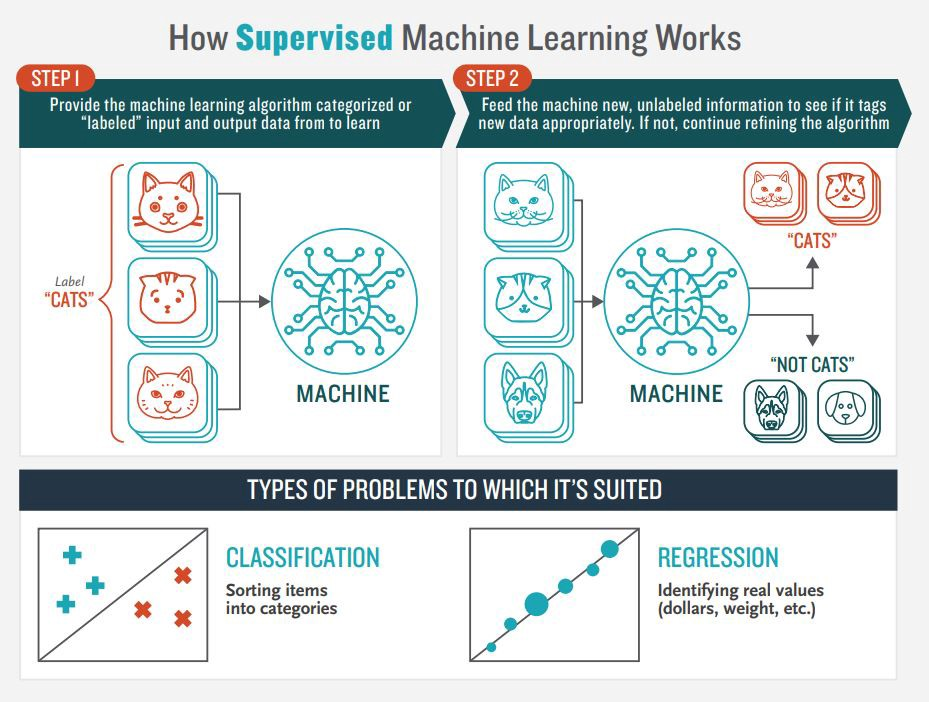
\includegraphics[width=1\textwidth]{figures/1174006/chapter1/supervisedlearning.jpeg}
	\centering
	\caption{Supervised Learning.}
\end{figure}
\noindent
Contoh algoritma yang digunakan pada supervised learning meliputi :
\begin{enumerate}
	\item Clasification (Categorical) and Regression (Numerical)
    \item Logistic Regression
    \item Model Ensemble
	\item Time series
\end{enumerate}

\subsubsection{Klasifikasi}
\hfill\break
Classification adalah tindakan untuk memberikan kelompok pada setiap keadaan. Setiap keadaan berisi sekelompok atribut, salah satunya adalah class attribute. Metode ini butuh untuk menemukan sebuah model yang dapat menjelaskan class attribute itu sebagai fungsi dari input attribute.
\begin{figure}[H]
	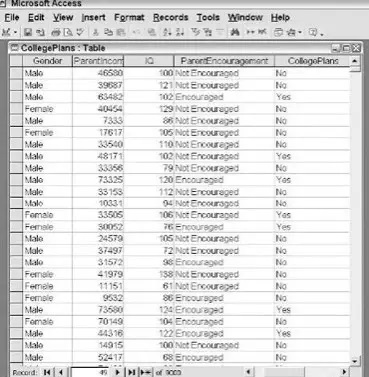
\includegraphics[width=1\textwidth]{figures/1174006/chapter1/clasification.jpg}
	\centering
	\caption{Clasification.}
\end{figure}
\noindent
Class adalah attribute CollegePlans yang berisi dua pernyataan, Yes dan No, perhatikan ini.
\noindent
Sebuah Classification Model akan menggunakan atribut lain dari kasus tersebut (input attribut; yaitu kolom IQ, Gender, ParentIncome, dan ParentEncouragement) untuk dapat menentukan pola (pattern) class (Output Attribute; yaitu Kolom CollegePlans yang berisi Yes atau No).
\noindent
Algoritma Data Mining yang membutuhkan variabel target untuk belajar (sampai mendapatkan rule / pola yang berlaku pada data tersebut) kita standarkan dengan sebuthan dengan Supervised Algorithm.
\noindent
Nah, yang termasuk kepada Classification Algorithm adalah Decision Trees, Neural Network dan Naives Bayes.
\subsubsection{Regresi}
\hfill\break
Metode Regression mirip dengan metode Classification, yang membedakannya adalah metode regression tidak bisa mencari pola yang dijabarkan sebagai class (kelas).
\noindent
Metoda regression bertujuan untuk mecari pola dan menentukan sebuah nilai numerik.
\noindent
Sebuah Teknik Linear Line-fitting sederhana adalah sebuah contoh dari Regression, dimana hasilnya adalah sebuah fungsi untuk menentukan hasil yang berdasarkan nilai dari input.
\noindent
Bentuk yang lebih canggih dari regression sudah mendukung input berupa kategori, jadi tidak hanya input berupa numerik. Teknik paling popular yang digunakan untuk regression adalah linear regression dan logistic regression. Teknik lain yang didukung oleh SQL Server Data mining adalah Regression Trees (bagian dari dari algoritma Microsoft Decission Trees) dan Neural Network.
\noindent
Regression digunakan untuk memecahkan banyak problem bisnis – contohnya untuk memperkirakan metode distribusi, kapasitas distribusi, musim dan untuk memperkirakan kecepatan angin berdasarkan temperatur, tekanan udara, dan kelembaban.
\subsubsection{Unsupervised Learning}
\hfill\break
Unsupervised learning memiliki keunggulan dari supervised learning. Jika supervised learning memiliki label sebagai dasar prediksi baik serta membuat clasification dan regression algorithm memungkinkan. Tetapi dalam realitanya, data real itu banyak yang tidak memiliki label. Label kebanyakan jika data sudah masuk ke ERP apapun bentuk ERPnya dan bagaimana kalo datanya berupa natural input seperti suara, gambar, dan video. Unsupervised learning tidak menggunakan label dalam memprediksi target feautures / variable. Melainkan menggunakan ke samaan dari attribut attribut yang dimiliki. Jika attribut dan sifat-sifat dari data data feature yang diekstrak memiliki kemirip miripan, maka akan dikelompok kelompokan (clustering). Sehingga hal ini akan menimbulkan kelompok kelompok (cluster). Jumlah cluster bisa unlimited. Dari kelompok kelompok itu model melabelkan, dan jika data baru mau di prediksi, maka akan dicocok kan dengan kelompok yang mirip mirip featurenya.
\begin{figure}[H]
	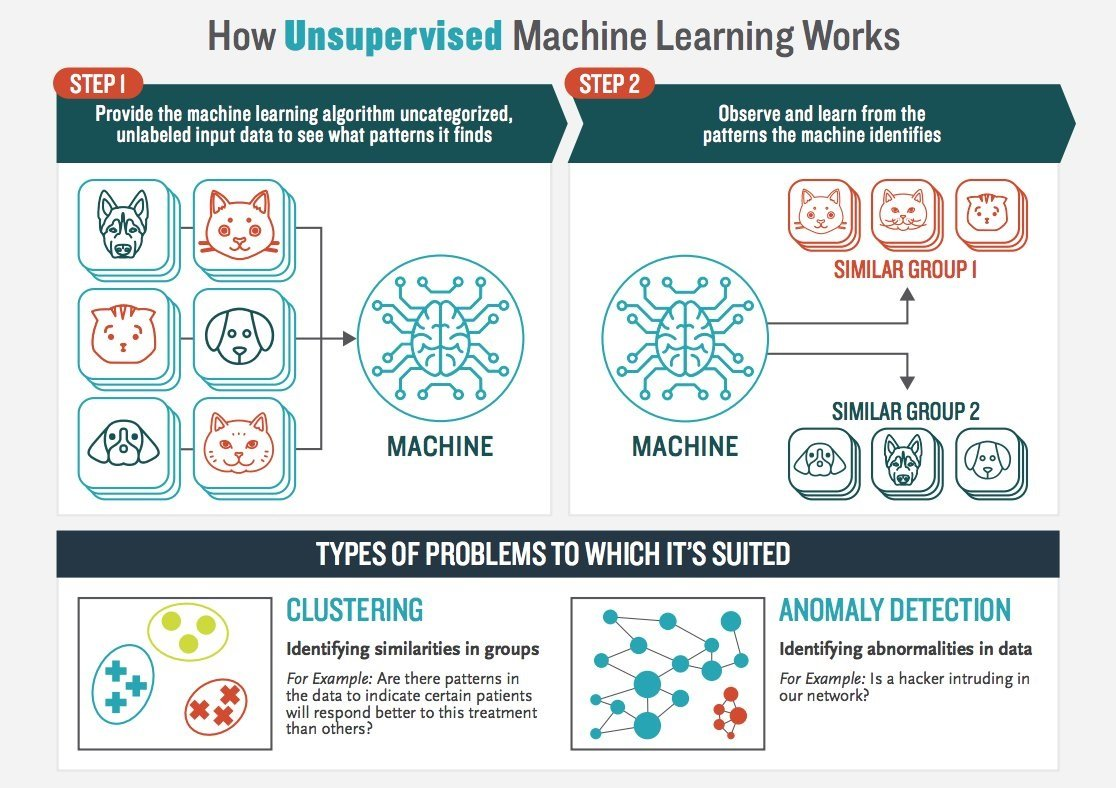
\includegraphics[width=1\textwidth]{figures/1174006/chapter1/unsupervisedlearning.jpg}
	\centering
	\caption{Unsupervised Learning.}
\end{figure}
\noindent
Tetapi unsupervise learning tidak memiliki outcome yang spesifik layaknya di supervise learning, hal ini dikarenakan tidak adanya ground truth / label dasar. Walaupun begitu, unsupervised learning masih dapat memprediksi dari ketidakadaan label dari kemiripan attribute yang dimilik data.
\noindent
Algoritma yang digunakan di unsupervised learning :
\begin{enumerate}
	\item Clustering
    \item Anomaly Detection
    \item Training Model
    \item Association Discovery
\end{enumerate}
\subsubsection{Data Set}
\hfill\break
Dataset adalah objek yang merepresentasikan data dan relasinya di memory. Strukturnya mirip dengan data di database. Dataset berisi koleksi dari datatable dan data relation.
\subsubsection{Training Set}
\hfill\break
Training set adalah bagian dataset yang kita latih untuk membuat prediksi atau menjalankan fungsi dari sebuah algoritma ML lainnya sesuai tujuannya masing-masing. Kita memberikan petunjuk melalui algoritma agar mesin yang kita latih bisa mencari korelasinya sendiri. 
\subsubsection{Testing Set}
\hfill\break
Test set adalah bagian dataset yang kita tes untuk melihat keakuratannya, atau dengan kata lain melihat performanya.
\subsection{Praktek}
\begin{enumerate}
	\item Instalasi  library  scikit  dari  anaconda,  mencoba  kompilasi  dan  uji  coba  ambil contoh kode dan lihat variabel explorer.
	
	\textbf{Instalasi Library Scikit-Learn dengan Anaconda}
	\begin{enumerate}
		\item Pertama pastikan anda telah menginstall Anaconda. Jika sudah menginstall Anaconda, jalankan Anaconda Navigator.
		\begin{figure}[H]
			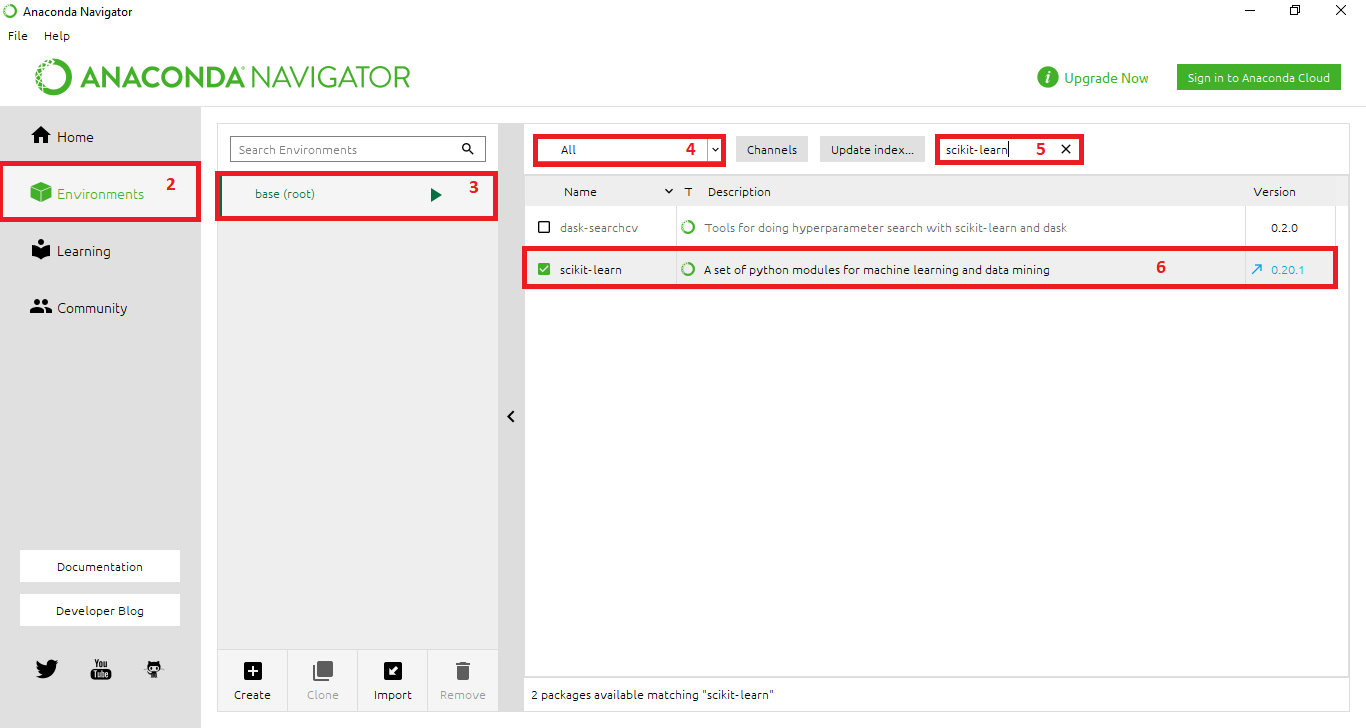
\includegraphics[width=1\textwidth]{figures/1174006/chapter1/praktek/install.png}
			\centering
			\caption{Instalasi Library Scikit-Learn.}
		\end{figure}
		\item Selanjutnya klik menu Environment.
		\item Kemudian klik environment base(root). Disini kita akan melakukan instalasi library scikit- learn di environment base(root).
		\item Lalu pilih All. Untuk menampilkan list library yang ada.
		\item Setelah itu cari scikit-learn di kolom pencarian.
		\item Selanjutnya centang library scikit-learn, lalu klik tombol Apply.
	\end{enumerate}

	\textbf{Mencoba Menggunakan Library scikit-Learn}
	\begin{enumerate}
		\item Pertama jalankan aplikasi Spyder.
		\item Kemudian buat file baru, lalu tambahkan kode berikut.
		\lstinputlisting[language=Python]{src/1174006/chapter1/contoh.py}
		\item Simpan dan jalankan.
		\item Hasil dari variabel explorernya sebagai berikut.
		\begin{figure}[H]
			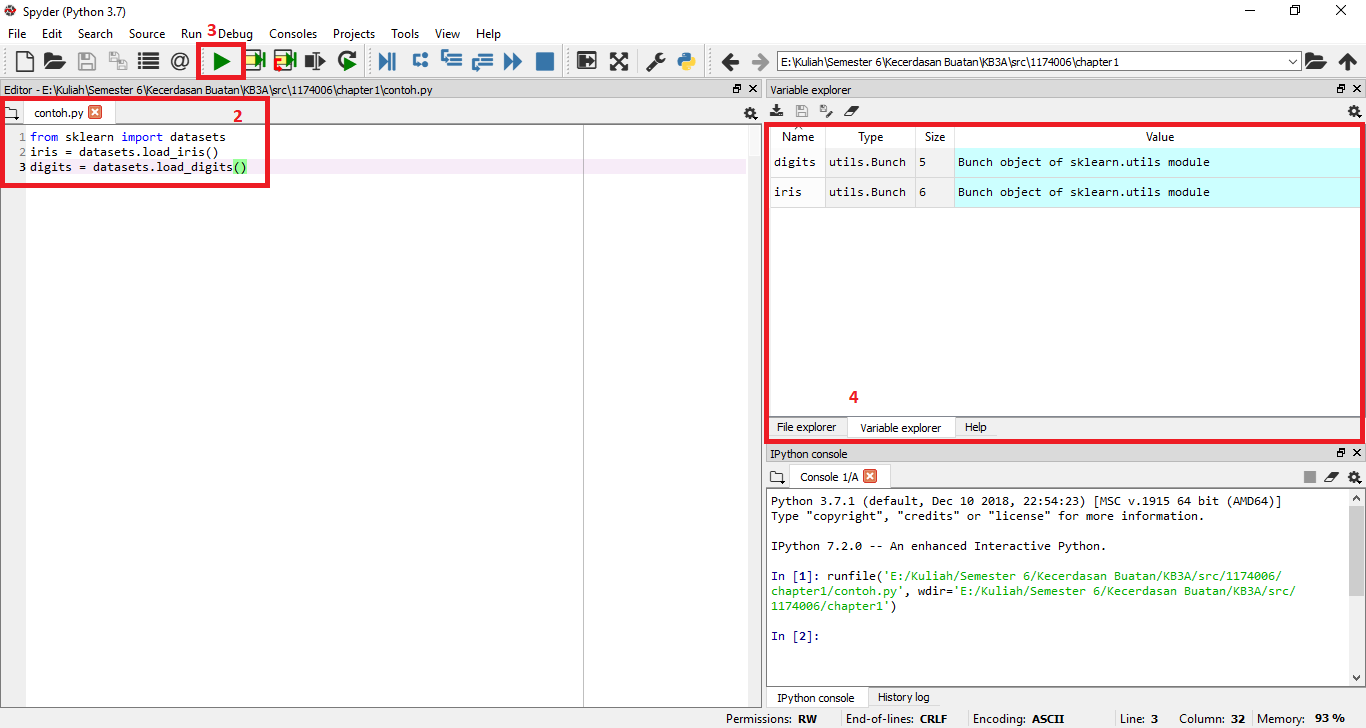
\includegraphics[width=1\textwidth]{figures/1174006/chapter1/praktek/variabel.png}
			\centering
			\caption{Variabel Explorer Library Scikit-Learn.}
		\end{figure}
	\end{enumerate}
	
	\item Mencoba Loading an example dataset, menjelaskan maksud dari tulisan terse-but dan mengartikan per baris.
	\lstinputlisting[language=Python]{src/1174006/chapter1/coba1.py}
	
	Hasilnya akan seperti ini.
	\begin{figure}[H]
		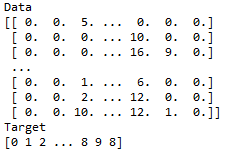
\includegraphics[width=5cm]{figures/1174006/chapter1/praktek/coba1.png}
		\centering
		\caption{Hasil Loading an Example Dataset.}
	\end{figure}

	\item Mencoba  Learning  and  predicting,  menjelaskan  maksud  dari  tulisan  tersebut dan mengartikan per baris.
	\lstinputlisting[language=Python]{src/1174006/chapter1/coba2.py}
	
	Hasilnya akan seperti ini.
	\begin{figure}[H]
		
\includegraphics[width=1cm]{figures/1174006/chapter1/praktek/coba2.png}
		\centering
		\caption{Hasil Learning and Predicting.}
	\end{figure}

	\item Mencoba Model persistence, menjelaskan maksud dari tulisan tersebut dan mengartikan per baris.
	\lstinputlisting[language=Python]{src/1174006/chapter1/coba3.py}
	
	Hasilnya akan seperti ini.
	\begin{figure}[H]
		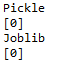
\includegraphics[width=2cm]{figures/1174006/chapter1/praktek/coba3.png}
		\centering
		\caption{Hasil Model Persistence.}
	\end{figure}

	\item Mencoba Conventions, menjelaskan maksud dari tulisan tersebut dan mengartikan per baris.
	\lstinputlisting[language=Python]{src/1174006/chapter1/coba4.py}
	
	Hasilnya akan seperti ini.
	\begin{figure}[H]
		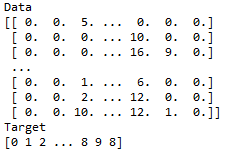
\includegraphics[width=5cm]{figures/1174006/chapter1/praktek/coba1.png}
		\centering
		\caption{Hasil Conventions.}
	\end{figure}

\end{enumerate}

\subsection{Penanganan Error}
\begin{enumerate}
	\item Skrinsut error.
	\begin{itemize}
		\item Name Error
		\hfill\break
		\begin{figure}[H]
			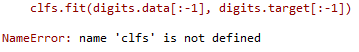
\includegraphics[width=1\textwidth]{figures/1174006/chapter1/error/err3.png}
			\centering
			\caption{Name Error.}
		\end{figure}
		\item Import Error
		\hfill\break
		\begin{figure}[H]
			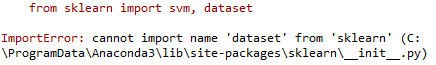
\includegraphics[width=1\textwidth]{figures/1174006/chapter1/error/err1.png}
			\centering
			\caption{Import Error.}
		\end{figure}
		\item Value Error
		\hfill\break
		\begin{figure}[H]
			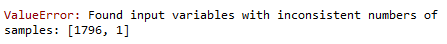
\includegraphics[width=1\textwidth]{figures/1174006/chapter1/error/err2.png}
			\centering
			\caption{Value Error.}
		\end{figure}
		\item Syntax Error
		\hfill\break
		\begin{figure}[H]
			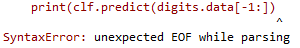
\includegraphics[width=1\textwidth]{figures/1174006/chapter1/error/err4.png}
			\centering
			\caption{Syntax Error.}
		\end{figure}
	\end{itemize}
	\item Tuliskan kode eror dan jenis errornya.
	\begin{itemize}
		\item Name Error
		\hfill\break
		Name Error adalah exception yang terjadi saat syntax melakukan eksekusi terhadap local name atau global name yang tidak terdefinisi.
		\item Import Error
		\hfill\break
		Import Error adalah exception yang terjadi saat syntax melakukan import terhadap library yang tidak terdefinisi.
		\item Value Error
		\hfill\break
		Value Error adalah exception yang terjadi saat syntax memiliki nilai yang tidak valid.
		\item Syntax Error
		\hfill\break
		Syntax Error adalah exception yang terjadi saat ada kesalahan dalam mengetikkan syntax.
	\end{itemize}
	\item Solusi pemecahan masalah error tersebut.
	\begin{itemize}
		\item Name Error
		\hfill\break
		Solusinya adalah memastikan variabel atau function yang dipanggil ada atau tidak salah ketik.
		\item Import Error
		\hfill\break
		Solusinya adalah memastikan library yang dipanggil ada atau tidak salah ketik.
		\item Value Error
		\hfill\break
		Solusinya adalah memastikan nilai yang diinputkan valid.
		\item Syntax Error
		\hfill\break
		Solusinya adalah memastikan syntax yang diketik tidak salah ketik.
	\end{itemize}
\end{enumerate}

\subsection{Bukti Tidak Plagiat}
\begin{figure}[H]
	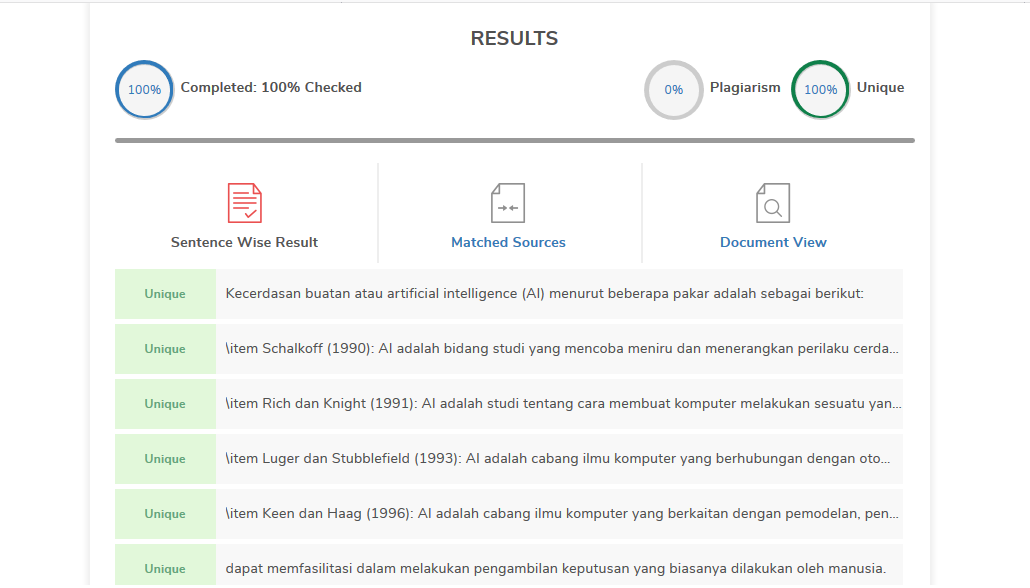
\includegraphics[width=1\textwidth]{figures/1174006/chapter1/plagiat.png}
	\centering
	\caption{Bukti Tidak Plagiat.}
\end{figure}
%\section{1174027 - Harun Ar - Rasyid}
\subsection{Teori}
\begin{enumerate}
	\item Sejarah dan Perkembangan
	\hfill\break
	Kecerdasan Buatan atau dalam Bahasa inggris sering disebut Artifical Intelligence yang sering disebut juga sebagai AI, pada 10 tahun lalu masyarakat belum terlalu mengetahui hal tersebut dan masih menjadi bahan candaan dikalangan masyarakat. Awal perkembangan AI dimulai pada tahun 1952-1969 yang dimulai dengan kesuksesan Newwll dan temannya simon menggunakan sebuah program yang disebut dengan General Problem Solver. Program ini dibangun untuk tujuan penyelesaiin masalah secara manusiawi. Pada tahun 1966-1974 perkembangan kecerdasan buatan mulai melambat. Ada 3 faktor utama yang menyebabkan hal itu terjadi:
	\begin{itemize}
		\item Banyak subjek pada program AI yang bermunculan hanya mengandung sedikit atau bahkan sama sekali tidak  mengandung sama sekali pengetahuan (knowledge).
		\item Kecerdasan buatan harus bisa menyelesaikan banyak masalah.
		\item Untuk menghasilkan perilkau intelijensia ada beberapa batasan pada struktur yang bisa digunakan.
	\end{itemize}
	Definisi kecerdasan buatan itu sendiri adalah suatu system teknologi yang didalamnya ditambahakan kecerdasan oleh manusia, kecerdasan buatan diatur dan dikembangkan dalam konteks ilmiah, dan bentukan dari kecerdasan entitas ilmiah yang ada.
	\item Definisi
	\hfill\break
	Supervised learning, klasifikasi, regresi, unsupervised learning, dataset, trainingset dan testingset.
	\begin{itemize}
		\item Supervised Learning
		\hfill\break
		Supervised Learning merupakan sebuah tipe learning yang mempunyai variable input dan variable output, tipe ini juga menggunakan satu algoritma atau lebih dari satu algoritma yang digunakan untuk mempelajari fungsi  pemetaan dari input ke output.
		\item Klasifikasi
		\hfill\break
		Klasifikasi adalah pengelompokan data di mana data yang digunakan memiliki label atau kelas target. Sehingga algoritma untuk menyelesaikan masalah klasifikasi dikategorikan ke dalam pembelajaran terbimbing.
		\item Regresi
		\hfill\break
		regressi metode analisis statistik yang digunakan untuk dapat melihat efek antara dua atau lebih variabel. Hubungan variabel dalam pertanyaan adalah fungsional yang diwujudkan dalam bentuk model matematika. Dalam analisis regresi, variabel dibagi menjadi dua jenis, yaitu variabel respons atau yang biasa disebut variabel dependen dan variabel independen atau dikenal sebagai variabel independen. Ada beberapa jenis analisis regresi, yaitu regresi sederhana yang mencakup linear sederhana dan regresi non-linear sederhana dan regresi berganda yang mencakup banyak linier atau non-linear berganda. Analisis regresi digunakan dalam pembelajaran mesin pembelajaran dengan metode pembelajaran terawasi.
		\item Unsupervised learning 
		\hfill\break
		unsupervised learning jenis pembelajaran di mana kita hanya memiliki data input (input data) tetapi tidak ada variabel output yang terkait. Tujuan dari pembelajaran tanpa pengawasan adalah untuk memodelkan struktur dasar atau distribusi data dengan tujuan mempelajari data lebih lanjut, dengan kata lain, itu adalah fungsi simpulan yang menggambarkan atau menjelaskan data.
		\item Data set
		\hfill\break
		Data set objek yang merepresentasikan data dan relasinya di memory. Strukturnya mirip dengan data di database. Dataset berisi koleksi dari datatable dan datarelation.
		\item Training Set
		\hfill\break
		Training set adalah bagian dari dataset yang di latih untuk membuat prediksi atau menjalankan fungsi dari algoritma ML lain sesuai dengan masing-masing. Memberikan instruksi melalui algoritma sehingga mesin yang di praktikkan dapat menemukan korelasinya sendiri.
		\item Testing Set
		\hfill\break
		testing set adalah bagian dari dataset yang kami uji untuk melihat akurasinya, atau dengan kata lain untuk melihat kinerjanya.
	\end{itemize}
\end{enumerate}
\subsection{Praktek}
\begin{enumerate}
	\item Instalasi Library scikit dari ianaconda, mencoba kompilasi dan uji coba ambil contoh kode dan lihat variabel explorer
	\hfill\break
	\begin{figure}[H]
		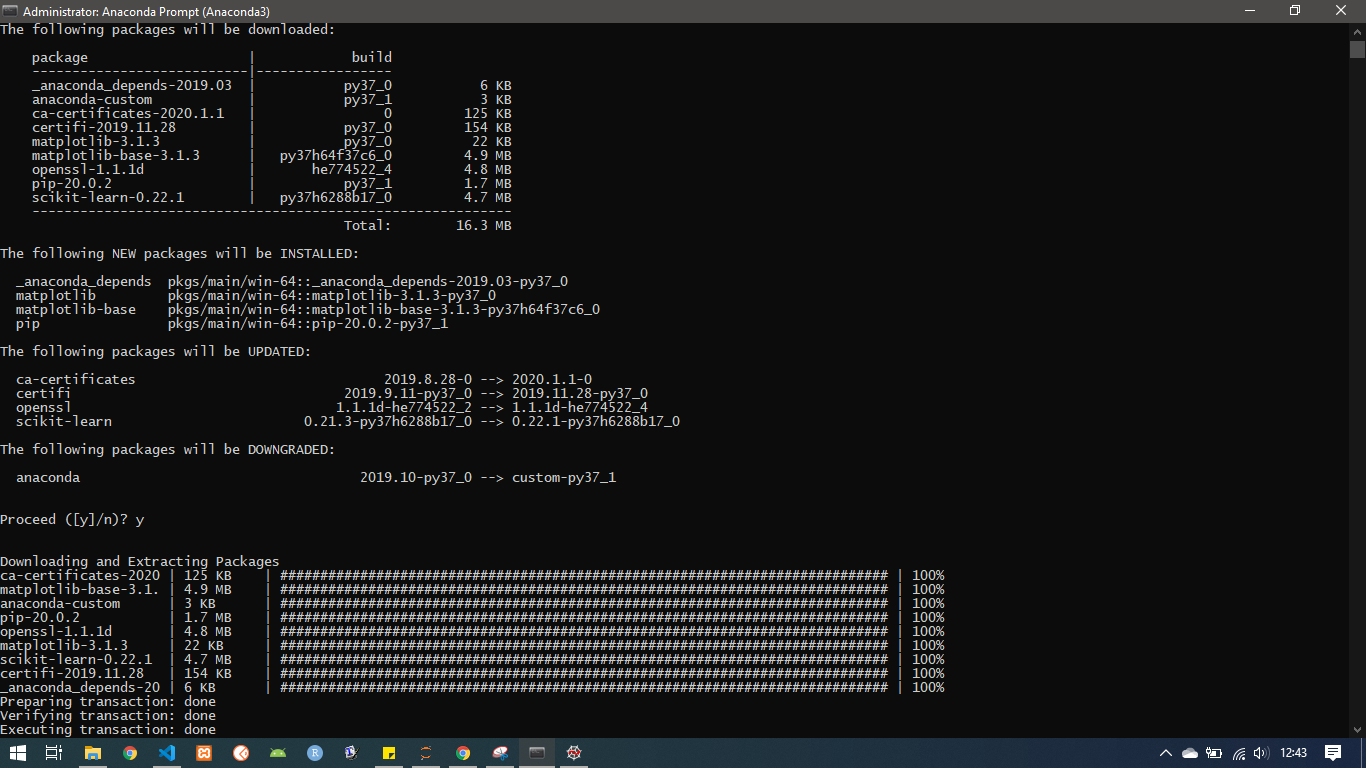
\includegraphics[width=4cm]{figures/1174027/1/instalasi.png}
		\centering
		\caption{Instalasi Package Scikit Learn}
	\end{figure}
	\begin{figure}[H]
		\includegraphics[width=4cm]{figures/1174027/1/variabel.png}
		\centering
		\caption{Isi Variabel Explorer}
	\end{figure}
	\item Mencoba loading an example dataset
	\hfill\break
	\lstinputlisting[firstline=7, lastline=11]{src/1174027/1/1174027.py}
	\item Mencoba Learning dan predicting
	\hfill\break
	\lstinputlisting[firstline=13, lastline=22]{src/1174027/1/1174027.py}
	\item Mencoba Model Persistence
	\hfill\break
	\lstinputlisting[firstline=25, lastline=34]{src/1174027/1/1174027.py}
	\item Mencoba Conventions
	\hfill\break
	\lstinputlisting[firstline=37, lastline=48]{src/1174027/1/1174027.py}
\end{enumerate}
\subsection{Penanganan Error}
\begin{enumerate}
	\item ScreenShoot Error
	\begin{figure}[H]
		\includegraphics[width=4cm]{figures/1174027/error/1_import.png}
		\centering
		\caption{Import Error}
	\end{figure}
	\begin{figure}[H]
		\includegraphics[width=4cm]{figures/1174027/error/1_value.png}
		\centering
		\caption{Value Error}
	\end{figure}
	\item Tuliskan Kode Error dan Jenis Error
	\begin{itemize}
		\item Import Error
		\item Value Error
	\end{itemize}
	\item Cara Penangan Error
	\begin{itemize}
		\item Import Error
		\hfill\break
		Dengan Menginstall Library Yang Tidak Ditemukan
		\item Value Error
		\hfill\break
		Mengubah Bentuk Arraynya, Menjadi 1 Dimensi
	\end{itemize}
\end{enumerate}
\subsection{Bukti Tidak Plagiat}
\begin{figure}[H]
	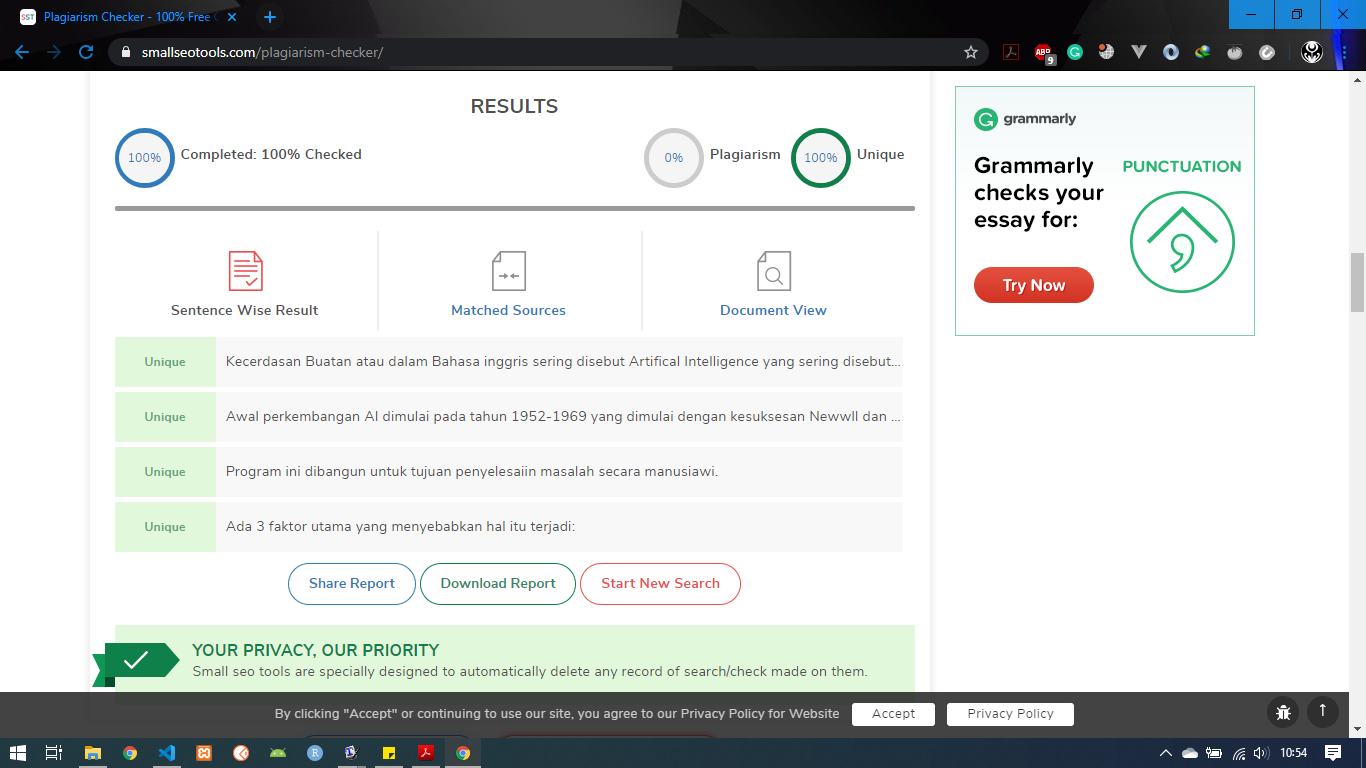
\includegraphics[width=4cm]{figures/1174027/bukti/1.png}
	\centering
	\caption{Bukti Tidak Melakukan Plagiat Chapter 1}
\end{figure}
%\section{1174031 - Muhammad Tomy Nur Maulidy}
\subsection{Teori}
\begin{enumerate}
	\item Sejarah dan Perkembangan
	\hfill\break
	Kecerdasan Buatan atau dalam Bahasa inggris sering disebut Artifical Intelligence yang sering disebut juga sebagai AI, pada 10 tahun lalu masyarakat belum terlalu mengetahui hal tersebut dan masih menjadi bahan candaan dikalangan masyarakat. Awal perkembangan AI dimulai pada tahun 1952-1969 yang dimulai dengan kesuksesan Newwll dan temannya simon menggunakan sebuah program yang disebut dengan General Problem Solver. Program ini dibangun untuk tujuan penyelesaiin masalah secara manusiawi. Pada tahun 1966-1974 perkembangan kecerdasan buatan mulai melambat. Ada 3 faktor utama yang menyebabkan hal itu terjadi:
	\begin{itemize}
		\item Banyak subjek pada program AI yang bermunculan hanya mengandung sedikit atau bahkan sama sekali tidak  mengandung sama sekali pengetahuan (knowledge).
		\item Kecerdasan buatan harus bisa menyelesaikan banyak masalah.
		\item Untuk menghasilkan perilkau intelijensia ada beberapa batasan pada struktur yang bisa digunakan.
	\end{itemize}
	Definisi kecerdasan buatan itu sendiri adalah suatu system teknologi yang didalamnya ditambahakan kecerdasan oleh manusia, kecerdasan buatan diatur dan dikembangkan dalam konteks ilmiah, dan bentukan dari kecerdasan entitas ilmiah yang ada.
	\item Definisi
	\hfill\break
	Supervised learning, klasifikasi, regresi, unsupervised learning, dataset, trainingset dan testingset.
	\begin{itemize}
		\item Supervised Learning
		\hfill\break
		Supervised Learning merupakan sebuah tipe learning yang mempunyai variable input dan variable output, tipe ini juga menggunakan satu algoritma atau lebih dari satu algoritma yang digunakan untuk mempelajari fungsi  pemetaan dari input ke output.
		\item Klasifikasi
		\hfill\break
		Klasifikasi adalah pengelompokan data di mana data yang digunakan memiliki label atau kelas target. Sehingga algoritma untuk menyelesaikan masalah klasifikasi dikategorikan ke dalam pembelajaran terbimbing.
		\item Regresi
		\hfill\break
		regressi metode analisis statistik yang digunakan untuk dapat melihat efek antara dua atau lebih variabel. Hubungan variabel dalam pertanyaan adalah fungsional yang diwujudkan dalam bentuk model matematika. Dalam analisis regresi, variabel dibagi menjadi dua jenis, yaitu variabel respons atau yang biasa disebut variabel dependen dan variabel independen atau dikenal sebagai variabel independen. Ada beberapa jenis analisis regresi, yaitu regresi sederhana yang mencakup linear sederhana dan regresi non-linear sederhana dan regresi berganda yang mencakup banyak linier atau non-linear berganda. Analisis regresi digunakan dalam pembelajaran mesin pembelajaran dengan metode pembelajaran terawasi.
		\item Unsupervised learning 
		\hfill\break
		unsupervised learning jenis pembelajaran di mana kita hanya memiliki data input (input data) tetapi tidak ada variabel output yang terkait. Tujuan dari pembelajaran tanpa pengawasan adalah untuk memodelkan struktur dasar atau distribusi data dengan tujuan mempelajari data lebih lanjut, dengan kata lain, itu adalah fungsi simpulan yang menggambarkan atau menjelaskan data.
		\item Data set
		\hfill\break
		Data set objek yang merepresentasikan data dan relasinya di memory. Strukturnya mirip dengan data di database. Dataset berisi koleksi dari datatable dan datarelation.
		\item Training Set
		\hfill\break
		Training set adalah bagian dari dataset yang di latih untuk membuat prediksi atau menjalankan fungsi dari algoritma ML lain sesuai dengan masing-masing. Memberikan instruksi melalui algoritma sehingga mesin yang di praktikkan dapat menemukan korelasinya sendiri.
		\item Testing Set
		\hfill\break
		testing set adalah bagian dari dataset yang kami uji untuk melihat akurasinya, atau dengan kata lain untuk melihat kinerjanya.
	\end{itemize}
\end{enumerate}
\subsection{Praktek}
\begin{enumerate}
	\item Instalasi Library scikit dari ianaconda, mencoba kompilasi dan uji coba ambil contoh kode dan lihat variabel explorer
	\hfill\break
	\begin{figure}[H]
		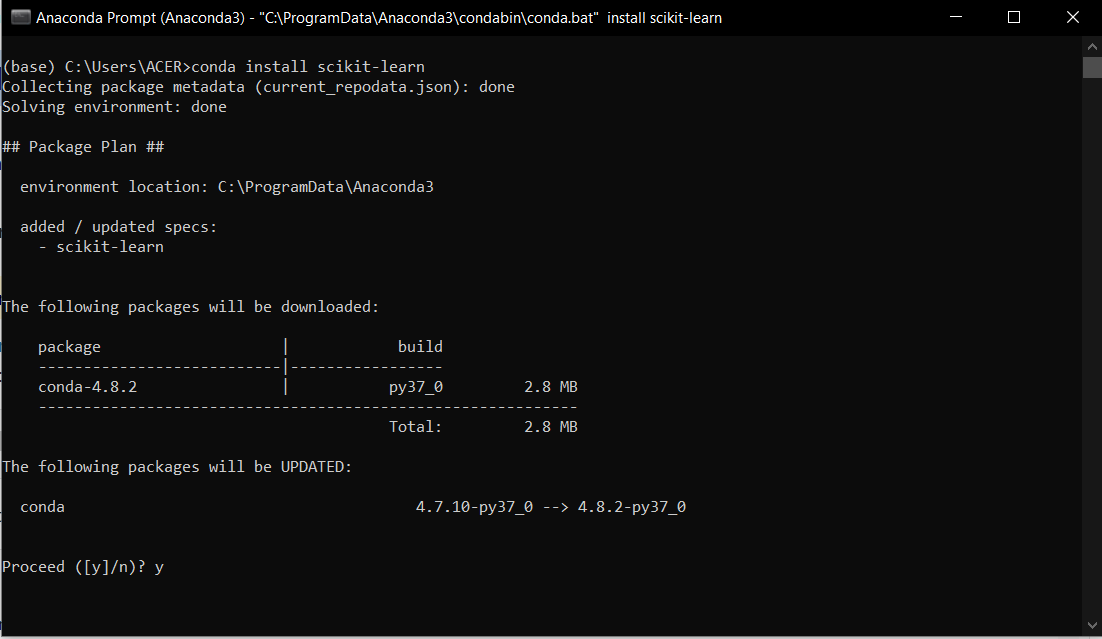
\includegraphics[width=4cm]{figures/1174031/1/1.PNG}
		\centering
		\caption{Instalasi Package Scikit Learn}
	\end{figure}
	\begin{figure}[H]
		\includegraphics[width=4cm]{figures/1174031/1/2.PNG}
		\centering
		\caption{Isi Variabel Explorer}
	\end{figure}
	\item Mencoba loading an example dataset
	\hfill\break
	\lstinputlisting[firstline=8, lastline=12]{src/1174031/1/1174031.py}
	\item Mencoba Learning dan predicting
	\hfill\break
	\lstinputlisting[firstline=14, lastline=24]{src/1174031/1/1174031.py}
	\item Mencoba Model Persistence
	\hfill\break
	\lstinputlisting[firstline=26, lastline=36]{src/1174031/1/1174031.py}
	\item Mencoba Conventions
	\hfill\break
	\lstinputlisting[firstline=38, lastline=50]{src/1174031/1/1174031.py}
\end{enumerate}
\subsection{Penanganan Error}
\begin{enumerate}
	\item ScreenShoot Error
	\begin{figure}[H]
		\includegraphics[width=4cm]{figures/1174031/1/error/1.png}
		\centering
		\caption{Import Error}
	\end{figure}
	\begin{figure}[H]
		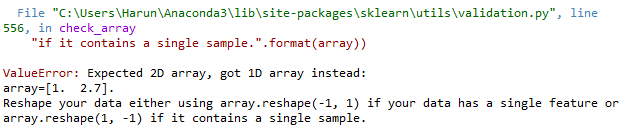
\includegraphics[width=4cm]{figures/1174031/1/error/2.png}
		\centering
		\caption{Value Error}
	\end{figure}
	\item Tuliskan Kode Error dan Jenis Error
	\begin{itemize}
		\item Import Error
		\item Value Error
	\end{itemize}
	\item Cara Penangan Error
	\begin{itemize}
		\item Import Error
		\hfill\break
		Dengan Menginstall Library Yang Tidak Ditemukan
		\item Value Error
		\hfill\break
		Mengubah Bentuk Arraynya, Menjadi 1 Dimensi
	\end{itemize}
\end{enumerate}
\subsection{Bukti Tidak Plagiat}
\begin{figure}[H]
	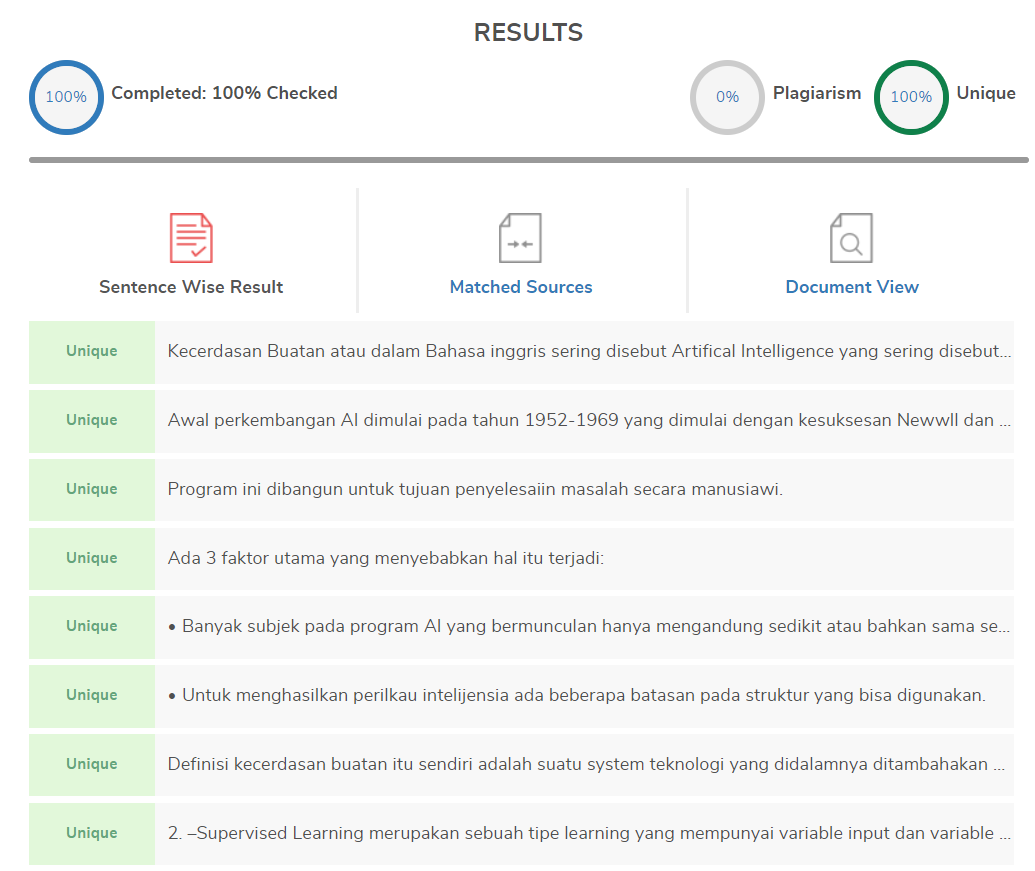
\includegraphics[width=4cm]{figures/1174031/1/plagiat/1.PNG}
	\centering
	\caption{Bukti Tidak Melakukan Plagiat 1}
    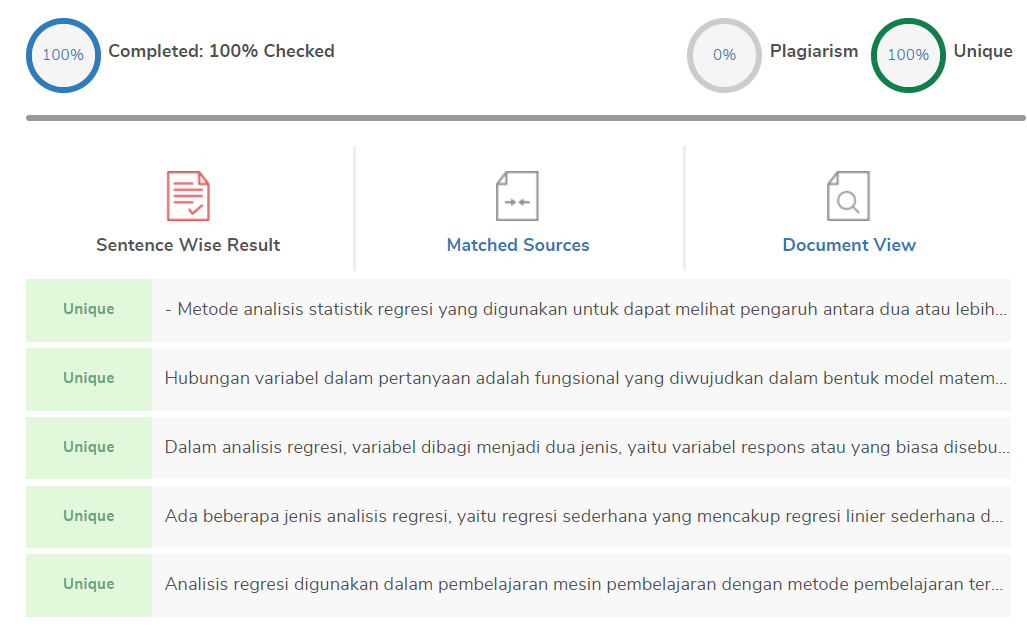
\includegraphics[width=4cm]{figures/1174031/1/plagiat/2.PNG}
	\centering
	\caption{Bukti Tidak Melakukan Plagiat 2}
\end{figure}
%\section{1174003 - Dwi Septiani Tsaniyah}
\subsection{Teori}
\begin{enumerate}
	\item Sejarah dan Perkembangan
	\hfill\break
	Kecerdasan buatan adalah bidang ilmu komputer yang sangat penting di masa kini dan masa depan untuk mewujudkan sistem komputer cerdas. "Intelligo" yang berarti "Saya mengerti". Berarti dasar kecerdasan untuk mengatasi dan mengambil tindakan. Sebenarnya, bidang Artificial Intelligence, atau disingkat AI, yang diambil dari tampilan komputer sekitar tahun 1940-an, sedangkan sejarah perkembangannya dapat ditelusuri sejak zaman Mesir kuno. Pada saat ini, perhatian diberikan pada kemampuan komputer untuk melakukan hal-hal yang dapat dilakukan manusia. Dalam hal ini, komputer dapat menggunakan kecerdasan dan komunikasi manusia McMulloh dan Pitts pada tahun 1943 meminta model matematika yang disebut perceptron neuron di otak. Mereka juga menunjukkan bagaimana neuron menjadi aktif seperti sakelar on-off dan neuron dapat belajar dan memberikan tindakan yang berbeda dari input yang diberikan. Kontribusi terbesar dalam bidang AI dimulai dengan karya Alan Turing, pada tahun 1950 yang mencoba menjawab "Can computer think" dengan menciptakan mesin Turing. Makalah Alan Turing tahun 1950 berjudul "Mesin Komputer dan Kecerdasan" membahas istilah-istilah mesin yang dianggap cerdas. Dia berasumsi bahwa jika sebuah mesin dapat berhasil berperilaku seperti manusia, kita dapat menganggapnya sebagai kecerdasan. Ada 3 faktor utama yang menyebabkan hal itu terjadi:
	\begin{itemize}
		\item Banyak subjek pada program AI yang bermunculan hanya mengandung sedikit atau bahkan sama sekali tidak  mengandung sama sekali pengetahuan (knowledge).
		\item Kecerdasan buatan harus bisa menyelesaikan banyak masalah.
		\item Untuk menghasilkan perilkau intelijensia ada beberapa batasan pada struktur yang bisa digunakan.
	\end{itemize}
	Definisi kecerdasan buatan itu sendiri adalah suatu system teknologi yang didalamnya ditambahakan kecerdasan oleh manusia, kecerdasan buatan diatur dan dikembangkan dalam konteks ilmiah, dan bentukan dari kecerdasan entitas ilmiah yang ada.
	\item Definisi
	\hfill\break
	Supervised learning, klasifikasi, regresi, unsupervised learning, dataset, trainingset dan testingset.
	\begin{itemize}
		\item Supervised Learning
		\hfill\break
		Supervised Learning merupakan sebuah tipe learning yang mempunyai variable input dan variable output, tipe ini juga menggunakan satu algoritma atau lebih dari satu algoritma yang digunakan untuk mempelajari fungsi  pemetaan dari input ke output.
		\item Klasifikasi
		\hfill\break
		Klasifikasi adalah pengelompokan data di mana data yang digunakan memiliki label atau kelas target. Sehingga algoritma untuk menyelesaikan masalah klasifikasi dikategorikan ke dalam pembelajaran terbimbing.
		\item Regresi
		\hfill\break
		regressi metode analisis statistik yang digunakan untuk dapat melihat efek antara dua atau lebih variabel. Hubungan variabel dalam pertanyaan adalah fungsional yang diwujudkan dalam bentuk model matematika. Dalam analisis regresi, variabel dibagi menjadi dua jenis, yaitu variabel respons atau yang biasa disebut variabel dependen dan variabel independen atau dikenal sebagai variabel independen. Ada beberapa jenis analisis regresi, yaitu regresi sederhana yang mencakup linear sederhana dan regresi non-linear sederhana dan regresi berganda yang mencakup banyak linier atau non-linear berganda. Analisis regresi digunakan dalam pembelajaran mesin pembelajaran dengan metode pembelajaran terawasi.
		\item Unsupervised learning 
		\hfill\break
		unsupervised learning jenis pembelajaran di mana kita hanya memiliki data input (input data) tetapi tidak ada variabel output yang terkait. Tujuan dari pembelajaran tanpa pengawasan adalah untuk memodelkan struktur dasar atau distribusi data dengan tujuan mempelajari data lebih lanjut, dengan kata lain, itu adalah fungsi simpulan yang menggambarkan atau menjelaskan data.
		\item Data set
		\hfill\break
		Data set objek yang merepresentasikan data dan relasinya di memory. Strukturnya mirip dengan data di database. Dataset berisi koleksi dari datatable dan datarelation.
		\item Training Set
		\hfill\break
		Training set adalah bagian dari dataset yang di latih untuk membuat prediksi atau menjalankan fungsi dari algoritma ML lain sesuai dengan masing-masing. Memberikan instruksi melalui algoritma sehingga mesin yang di praktikkan dapat menemukan korelasinya sendiri.
		\item Testing Set
		\hfill\break
		testing set adalah bagian dari dataset yang kami uji untuk melihat akurasinya, atau dengan kata lain untuk melihat kinerjanya.
	\end{itemize}
\end{enumerate}
\subsection{Praktek}
\begin{enumerate}
	\item Instalasi Library scikit dari ianaconda, mencoba kompilasi dan uji coba ambil contoh kode dan lihat variabel explorer
	\hfill\break
	\begin{figure}[H]
		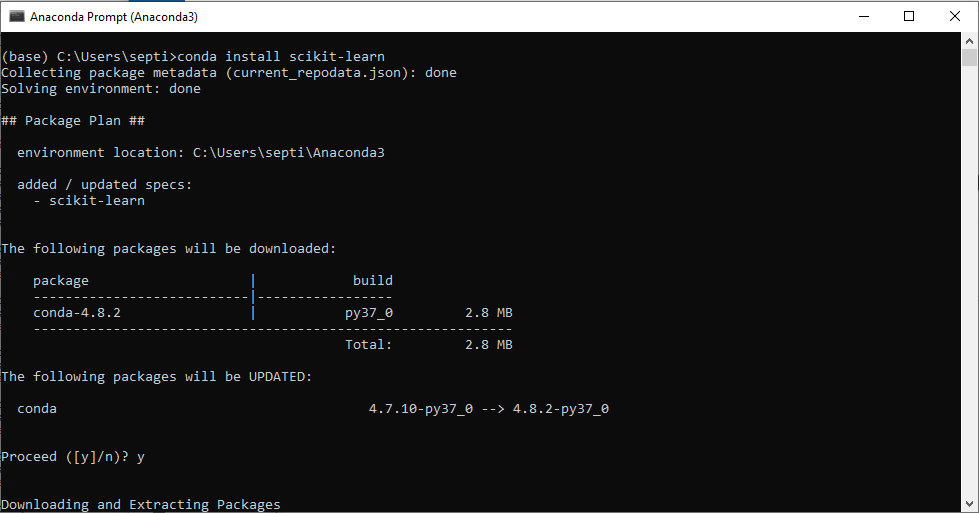
\includegraphics[width=4cm]{figures/1174003/1/1.PNG}
		\centering
		\caption{Instalasi Package Scikit Learn}
	\end{figure}
	\begin{figure}[H]
		\includegraphics[width=4cm]{figures/1174003/1/2.PNG}
		\centering
		\caption{Isi Variabel Explorer}
	\end{figure}
	\item Mencoba loading an example dataset
	\hfill\break
	\lstinputlisting[firstline=8, lastline=12]{src/1174003/1/1174003.py}
	\item Mencoba Learning dan predicting
	\hfill\break
	\lstinputlisting[firstline=14, lastline=24]{src/1174003/1/1174003.py}
	\item Mencoba Model Persistence
	\hfill\break
	\lstinputlisting[firstline=26, lastline=36]{src/1174003/1/1174003.py}
	\item Mencoba Conventions
	\hfill\break
	\lstinputlisting[firstline=38, lastline=50]{src/1174003/1/1174003.py}
\end{enumerate}
\subsection{Penanganan Error}
\begin{enumerate}
	\item ScreenShoot Error
	\begin{figure}[H]
		\includegraphics[width=4cm]{figures/1174031/1/error/1.png}
		\centering
		\caption{Import Error}
	\end{figure}
	\begin{figure}[H]
		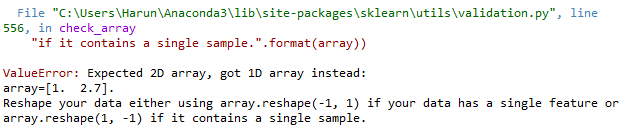
\includegraphics[width=4cm]{figures/1174031/1/error/2.png}
		\centering
		\caption{Value Error}
	\end{figure}
	\item Tuliskan Kode Error dan Jenis Error
	\begin{itemize}
		\item Import Error
		\item Value Error
	\end{itemize}
	\item Cara Penangan Error
	\begin{itemize}
		\item Import Error
		\hfill\break
		Dengan Menginstall Library Yang Tidak Ditemukan
		\item Value Error
		\hfill\break
		Mengubah Bentuk Arraynya, Menjadi 1 Dimensi
	\end{itemize}
\end{enumerate}
\subsection{Bukti Tidak Plagiat}
\begin{figure}[H]
	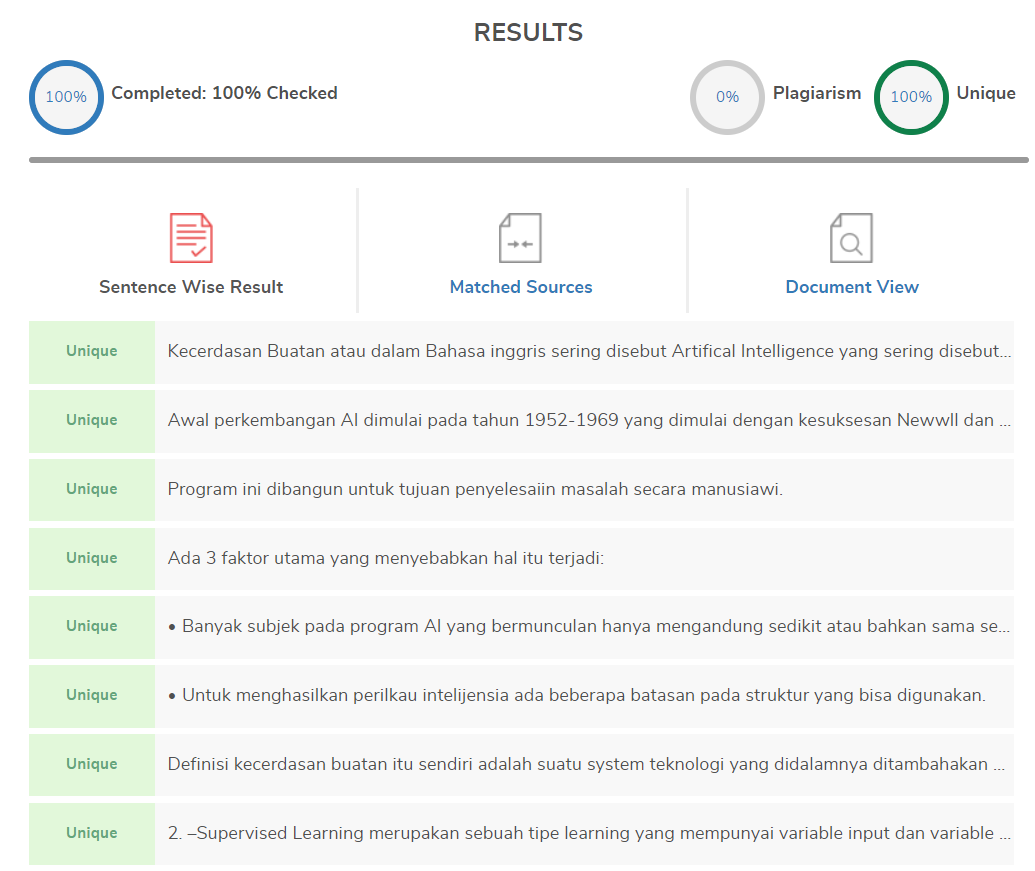
\includegraphics[width=4cm]{figures/1174031/1/plagiat/1.PNG}
	\centering
	\caption{Bukti Tidak Melakukan Plagiat 1}
\end{figure}
%\section{1174051 - Evietania Charis Sujadi}
\subsection{Teori}
\begin{enumerate}
\item Definisi, sejarah, dan juga pengembangan Kecerdasan Buatan
\subitem Definisi kecerdasan diciptakan oleh pengetahuan yang dapat membuat komputer untuk kecerdasan manusia terkait dengan penangkapan, pemodelan, dan penyimpanan kecerdasan manusia dalam suatu sistem teknologi. Contohnya adalah melakukan analisis penalti untuk menarik kesimpulan atau menerjemahkan kelemahan atau memutuskan dari satu bahasa ke bahasa lain.
\subitem Sejarah dan perkembangan intelijen terjadi pada musim panas 1956 menerima seminar tentang AI di Darmouth College. Seminar dihadiri oleh para ahli komputer dan membahas potensi komputer dalam pengaduan kecerdasan manusia. Namun, perkembangan yang sudah sering terjadi sejak LISP diciptakan, yaitu kecerdasan buatan yang dibuat pada tahun 1960 oleh John McCarthy. Istilah kecerdasan buatan atau Inteligensi Buatan diambil dari Marvin Minsky dari MIT. Dia menulis sebuah makalah ilmiah yang berjudul Steps to Artificial Intelligence, Institute for Proceedings of Radio Engineers 49, Januari 1961. 
\item  Definisi supervised learning, klasifikasi, regresi, dan unsupervised learning. Data set, training set dan testing set. 
\subitem Supervised learning merupakan sebuah pendekatan dimana sudah terdapat data yang dilatih, dan terdapat variable yang ditargetkan sehingga tujuan dari pendekatan ini adalah mengkelompokan suatu data ke data yang sudah ada. Sedangkan unsupervised learning tidak memiliki data latih, sehingga dari data yang ada, kita mengelompokan data tersebut menjadi 2 bagian atau 3 bagian dan seterusnya.
\subitem Klasifikasi adalah salah satu topik utama dalam data mining atau machine learning. Klasifikasi yaitu suatu pengelompokan data dimana data yang digunakan tersebut mempunyai kelas label atau target.
\subitem Regresi adalah Supervised learning tidak hanya mempelajari classifier, tetapi juga mempelajari fungsi yang dapat memprediksi suatu nilai numerik. Contoh, ketika diberi foto seseorang, kita ingin memprediksi umur, tinggi, dan berat orang yang ada pada foto tersebut.
\subitem Data set adalah cabang aplikasi dari Artificial Intelligence/Kecerdasan Buatan yang fokus pada pengembangan sebuah sistem yang mampu belajar sendiri tanpa harus berulang kali di program oleh manusia.
\subitem Training set yaitu jika pasangan objek, dan kelas yang menunjuk pada objek tersebut adalah suatu contoh yang telah diberi label akan menghasilkan suatu algoritma pembelajaran.
\subitem Tujuan dari set tes adalah untuk menentukan sejauh mana classifier berhasil membuat klasifikasi dengan benar
\end{enumerate}
\subsection{Instalasi}
\begin{enumerate}
\item {Instalasi Library Scikit}
Masuk pada windows lalu search "conda" , setelah itu akan muncul Anaconda prompt. lalu ketikkan conda install scikit-learn
\begin{figure}[ht]
\centering
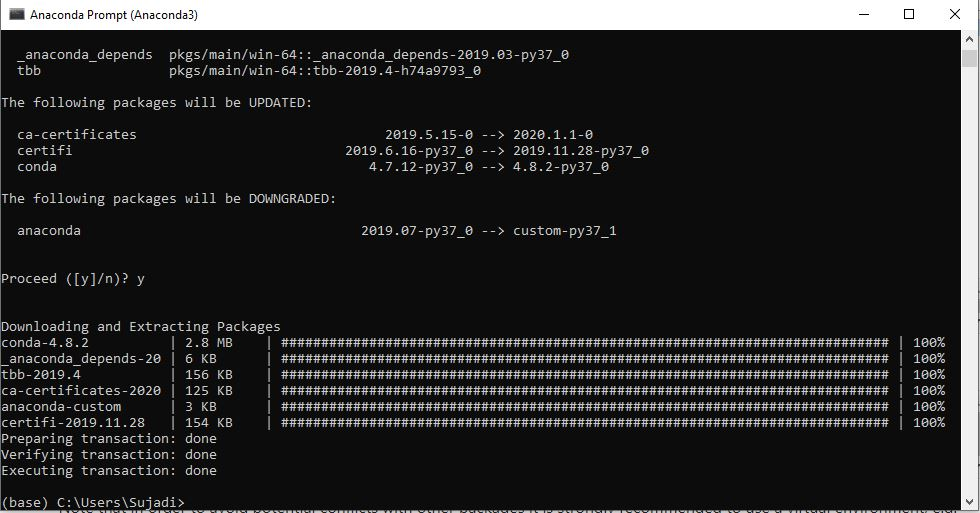
\includegraphics[scale=0.5]{figures/1174051/1/1.JPG}
\caption{Installasi}
\label{contoh}
\end{figure}
\begin{figure}[H]
\centering
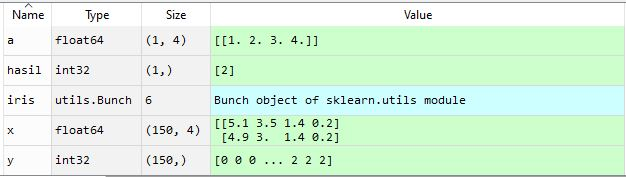
\includegraphics[width=4cm]{figures/1174051/1/2.JPG}
\caption{Isi Variabel Explorer}
\end{figure}
\item Mencoba loading an example dataset
\hfill\break
\lstinputlisting[firstline=8, lastline=12]{src/1174051/1/1174051.py}
\item Mencoba Learning dan predicting
\hfill\break
\lstinputlisting[firstline=14, lastline=24]{src/1174051/1/1174051.py}
\item Mencoba Model Persistence
\hfill\break
\lstinputlisting[firstline=26, lastline=36]{src/1174051/1/1174051.py}
\item Mencoba Conventions
\hfill\break
\lstinputlisting[firstline=38, lastline=50]{src/1174051/1/1174051.py}
\end{enumerate}
\subsection{Penanganan Error}
\begin{enumerate}
\item ScreenShoot Error
\begin{figure}[H]
	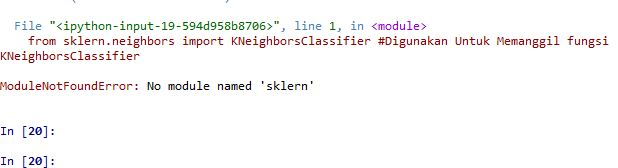
\includegraphics[width=4cm]{figures/1174051/1/error/1.JPG}
	\centering
	\caption{Import Error}
\end{figure}
\item Tuliskan Kode Error dan Jenis Error
\begin{itemize}
	\item ModuleNotFoundError
\end{itemize}
\item Cara Penangan Error
\begin{itemize}
	\item ModuleNotFoundError
	\hfill\break
	Typo pada pemanggilan sklearn
\end{itemize}
\end{enumerate}
\subsection{Bukti Tidak Plagiat}
\begin{figure}[H]
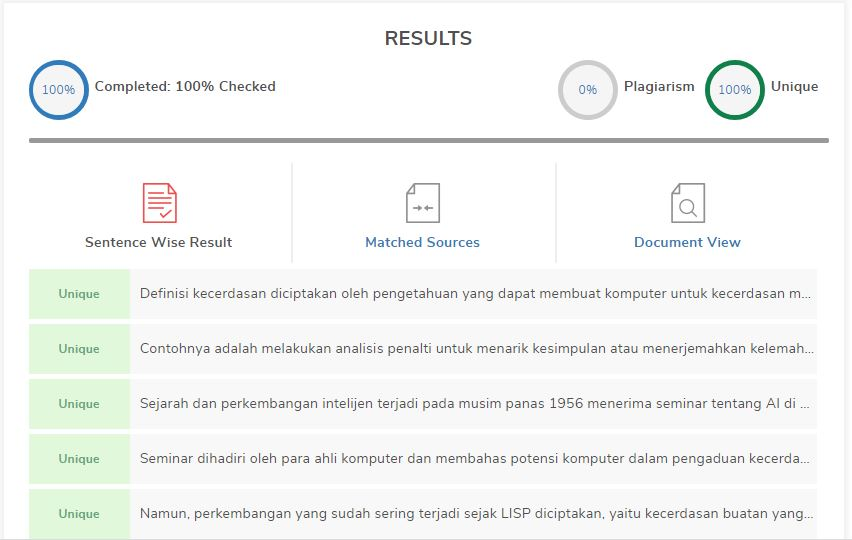
\includegraphics[width=4cm]{figures/1174051/1/plagiat/1.JPG}
\centering
\caption{Bukti Tidak Melakukan Plagiat 1}
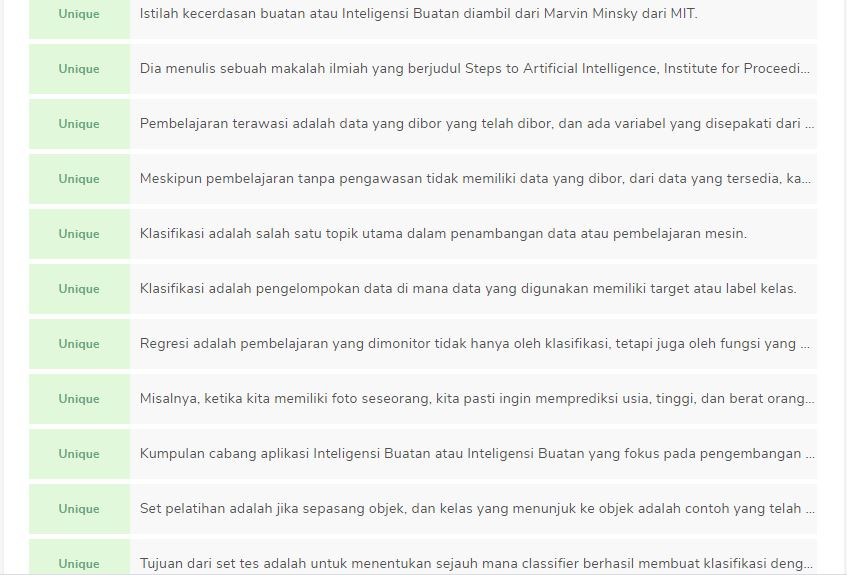
\includegraphics[width=4cm]{figures/1174051/1/plagiat/2.JPG}
\centering
\caption{Bukti Tidak Melakukan Plagiat 2}
\end{figure}
%\section{1174021 - Muhammad Fahmi}
\subsection{Teori}
\begin{enumerate}

	\item Defenisi Kecerdasan Buatan
	\hfill\break
	Kecerdasan buatan yang jika dalam bahasa inggris ialah Artificial Intelligence (AI) adalah bagian dari ilmu komputer. Dengan penelitian dan pengembangan kecerdasan buatan, ia berusaha untuk tidak hanya berhasil tetapi untuk melengkapi pemikiran manusia dengan program komputer belajar mandiri. AI juga sudah banyak di aplikasikan di dunia bisnis, misalnya, dalam Google Maps. dan Istilah dalam AI juga sudah tidak asing lagi yaitu "Neural Network" dan "Deep learning" yang terkait dengan pengembangan kecerdasan buatan.

	\begin{figure}[H]
	\centering
		
\includegraphics[width=4cm]{figures/1174021/tugas1/materi/1.jpg}
		\caption{Kecerdasan Buatan.}
	\end{figure}

	\item Sejarah dan Perkembangan
	\hfill\break
	Pada tahun 1950 yang bertempat di AS kecerdasan buatan atau AI itu dimulai pada konferensi ilmiah di Dartmouth, M. Minsky, J.McCarthy, A. Newell, dan HA Simon adalah yang pertama berbicara tentang "kecerdasan buatan." Definisi yang sering dikutip untuk kecerdasan buatan diberikan oleh salah satu pendiri subjek, Marvin Minsky, pada tahun 1966: "Kecerdasan Buatan adalah ilmu membuat mesin melakukan hal-hal yang membutuhkan kecerdasan jika dilakukan oleh manusia." Jadi, ditentukan bahwa kecerdasan buatan adalah ilmu dan kedua mesin dapat mengambil alih pekerjaan manusia yang membutuhkan kecerdasan manusia. Adapun mengapa AI yaitu untuk pemecah an masalah umum dari para peneliti Newell, Shaw, dan Simon pada tahun 1960-an. Penelitian ini dapat memecahkan masalah sederhana. Namun, hasil penelitian tersebut tidak dapat digeneralisasi. Pada akhir 1960-an, program lain ditulis dengan ELIZA. Dengan demikian, Joseph Weizenbaum, seorang peneliti MIT,simulasikan sesi terapi. Pada tahun-tahun berikutnya, sains muda terus dikembangkan, yang diproduksi oleh MYCIN pada awal 1970-an dalam sistem inovatif lain berbasis AI. MYCIN dapat membantu dokter mendiagnosis.
	

	\item Kecerdasan buatan terbagi atas beberapa metode yaitu:
	\hfill\break
	Supervised learning, Unsupervised Learning, Klasifikasi, Regresi, Dataset, Trainingset dan juga Testingset.
	\begin{itemize}
		\item Supervised Learning
		\hfill\break
		Sebuah algoritma pembelajaran mesin yang dapat menerapkan informasi yang sudah ada dalam data dengan memberikan label tertentu, misalnya data yang telah diklasifikasikan sebelumnya (diarahkan). Algoritma ini mampu memberikan target untuk output yang dilakukan dengan membandingkan pengalaman belajar masa yang sudah lampau.
		\item Unsupervised Learning 
		\hfill\break
		Berbeda dengan Supervised Learning, Unsupervised Learning ialah sebuah pembelajaran mesin tanpa pengawasan adalah pembelajaran mesin yang digunakan pada data yang tidak memiliki informasi yang dapat diterapkan secara langsung (tidak diarahkan). Algoritma ini diharapkan dapat menemukan struktur tersembunyi dalam data yang tidak berlabel.
		\item Klasifikasi
		\hfill\break
		Klasifikasi adalah sampel milik dua kelas atau lebih dan ingin belajar dari data yang sudah diberi label cara memprediksi kelas data yang tidak berlabel. Contoh masalah klasifikasi adalah pengenalan digit tulisan tangan, di mana tujuannya adalah untuk menetapkan masing-masing vektor input ke salah satu dari sejumlah kategori diskrit. 
		\item Regresi
		\hfill\break
		Regrasi ialah sebuah metode untuk mengembangkan model (persamaan) yang menjelaskan hubungan antara beberapa variabel. Output dari analisis regresi adalah persamaan regresi. Dalam model regresi variabel dibagi menjadi dua bagian, yaitu variabel respon atau yang biasa juga disebut variabel dependen dan variabel explanatory atau juga biasa disebut variabel prediktor atau disebut juga variabel independen.
		\item Data set
		\hfill\break
		Dataset adalah sebuah kumpulan data atau objek dan bagaimana relasi dalam memori. Struktur Dataset mirip dengan data di dalam database. Dataset berisi koleksi dari datatable maupun data relasi.
		\item Training Set
		\hfill\break
		Training set ialah bagian dari dataset yang berfungsi untuk membuat prediksi atau mengatur fungsi dari algoritma-algoritma yang ada. Fungsi nya yang lain juga ada sesuai tujuannya masing-masing. Trainingset memberikan instruksi melalui algoritma sehingga mesin dapat mengerti dan membuat kolerasi sendiri.		
		\item Testing Set
		\hfill\break
		Sama seperti training set, testing set juga bagian dari dataset yang berfungsi menguji untuk melihat akurasinya, atau bisa juga untuk melihat suatu kinerja atau performa.
	\end{itemize}
\end{enumerate}
\subsection{Praktek}
\begin{enumerate}
	\item Instalasi Library scikit dari Anaconda, mencoba kompilasi dan uji coba ambil contoh kode dan lihat variabel explorer
	\hfill\break
	\begin{figure}[H]
		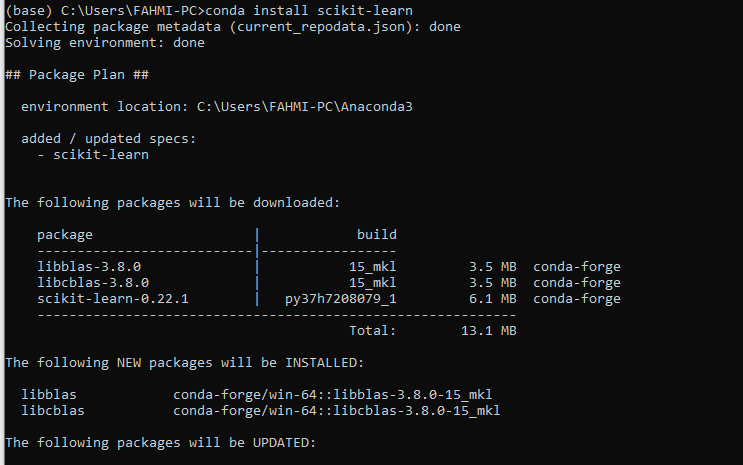
\includegraphics[width=4cm]{figures/1174021/tugas1/materi/2.PNG}
		\centering
		\caption{Instalasi Library Scikit Learn}
	\end{figure}
	\begin{figure}[H]
		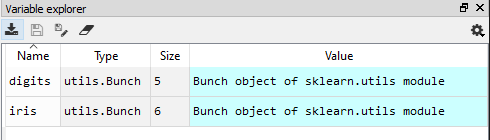
\includegraphics[width=4cm]{figures/1174021/tugas1/materi/3.PNG}
		\centering
		\caption{Isi Variabel Explorer}
	\end{figure}
	\item Uji coba loading an example dataset
	\hfill\break
	\lstinputlisting[firstline=10, lastline=14]{src/1174021/tugas1.py}
	\item Uji coba Learning dan predicting
	\hfill\break
	\lstinputlisting[firstline=18, lastline=21]{src/1174021/tugas1.py}
	\item Uji coba Model Persistence
	\hfill\break
	\lstinputlisting[firstline=25, lastline=41]{src/1174021/tugas1.py}
	\item Uji coba Conventions
	\hfill\break
	\lstinputlisting[firstline=44, lastline=56]{src/1174021/tugas1.py}
\end{enumerate}
\subsection{Penanganan Error}
\begin{enumerate}
	\item ScreenShoot Error
	\begin{figure}[H]
		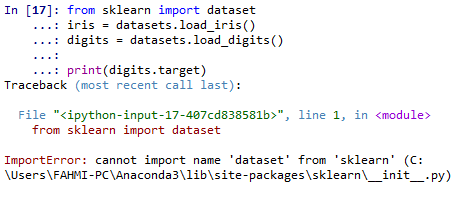
\includegraphics[width=4cm]{figures/1174021/tugas1/error/1.PNG}
		\centering
		\caption{Import Error}
	\end{figure}
	\begin{figure}[H]
		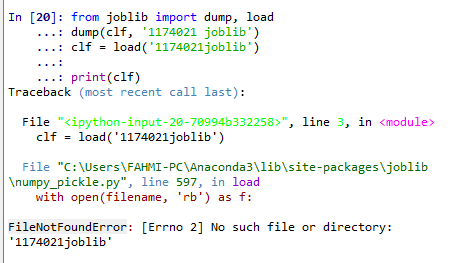
\includegraphics[width=4cm]{figures/1174021/tugas1/error/2.PNG}
		\centering
		\caption{FileNotFoundError}
	\end{figure}
	\item Tuliskan Kode Error dan Jenis Error
	\begin{itemize}
		\item Import Error
		\item FileNotFoundError
	\end{itemize}
	\item Cara Penangan Error
	\begin{itemize}
		\item Import Error
		\hfill\break
		Error terdapat typo pada dataset, seharusnya datasets
		\item FileNotFoundError
		\hfill\break
		Error terdapat pada 1174021joblib, tidak ada file yang dibaca, seharusnya 1174021.joblib
	\end{itemize}
\end{enumerate}
\subsection{Bukti Tidak Plagiat}
\begin{figure}[H]
	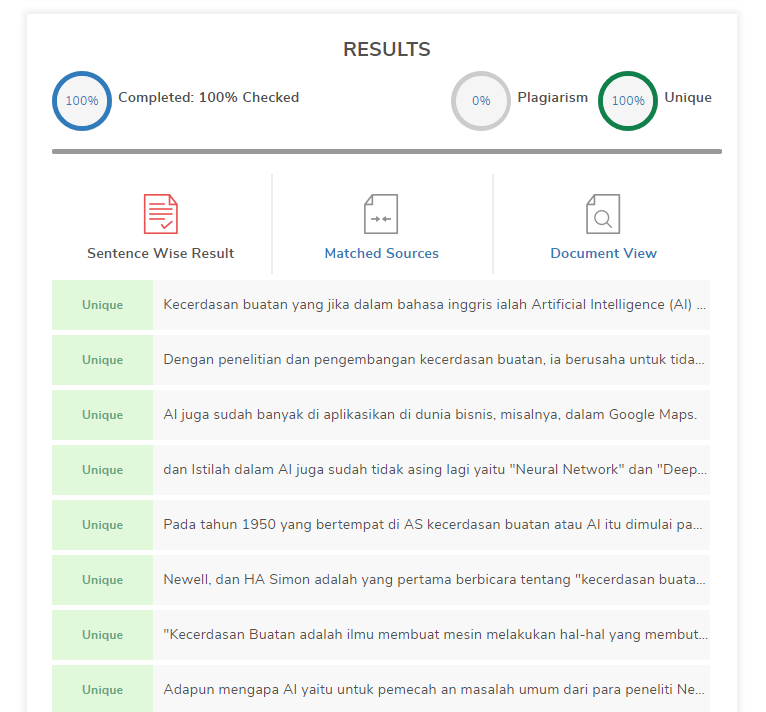
\includegraphics[width=4cm]{figures/1174021/tugas1/buktiplagiat/1.PNG}
	\centering
	\caption{Bukti Tidak Melakukan Plagiat Chapter 1}
\end{figure}
%\section{1174096 - Nico Ekklesia Sembiring}
\subsection{Teori}
\begin{enumerate}
	\item Pengetian, Sejarah dan Perkembangan Kecerdasan Buatan
	\hfill\break
    Kecerdasan buatan (Artificial Inteligence) merupakan suatu entitas yang cerdas secara ilmiah yang merupakan hasil dari gagasan dan ciptaan manusia. Suatu entitas dimasukkan kedalam suatu alat atau mesin sehingga membuat alat atau mesin itu dapat seolah-olah dapat berpikir dan mengambil keputusan sendiri. Kecerdasan buatan berbeda dengan perangkat computer, dimana computer melakukan pengambilan keputusan dan melakukan fungsi fungsi hanmya pada saat diarahkan oleh pengguna, tidak dapat melakukan secara otomatis. 
    \hfill\break
    Kecerdasan buatan dapat mengambil keputusan secara otomatis berdasarkan pengalaman yang telah sebelumnya terjadi dan direkam dan disimpan pada database perangkat kecerdasan buatan. Rekaman aktifitas yang telah dilakukan tersebut dapat diterapkan dikemudian hari ketika diperlukan. Kehadiran perangkat yang menggunakan kecerdasan buatan pada masa sekarang ini merupakan suatu kemajuan dalam bidang teknologi yang paling baik, dimana konsep perangkat yang menggunakan kecerdasan buatan sudah mulai dimanfaatkan dalam berbagai bidang seperti multimedia, mesin pencari, robotic, dan lain lain. 
    \hfill\break
    Komputer dapat dibuat menjadi entitas yang cerdas dengan menyediakan data dalam database. Selain diberi data, komputer juga dapat diberikan suatu kemampuan dalam mempelajari data. Pelatihan dan pembelajaran data ini akan membuat sistem dapat menentukan keputusan dan melakukan tugas untuk membuatnya lebih mudah bagi manusia di masa depan.
    \hfill\break
    Jarvis memiliki kemampuan berbicara memiliki kemampuan untuk mendeteksi kondisi kesehatan dan melakukan hal-hal lain yang diperintahkan oleh penciptanya. Ini disebabkan oleh kecerdasan Jarvis yang sudah sangat terlatih. Komputer pintar seperti jarvis diharapkan dapat ditemukan di masa depan sehingga banyak orang berlomba untuk mengembangkannya sekarang.
    \hfill\break


	Definisi kecerdasan buatan itu sendiri adalah suatu system teknologi yang didalamnya ditambahakan kecerdasan oleh manusia, kecerdasan buatan diatur dan dikembangkan dalam konteks ilmiah, dan bentukan dari kecerdasan entitas ilmiah yang ada.
	\item defenisi dari Supervised learning, klasifikasi, regresi, unsupervised learning, dataset, trainingset dan testingset.
	\begin{itemize}
		\item Supervised Learning
		\hfill\break
		Supervised Learning merupakan sebuah tipe learning yang mempunyai variable input dan variable output, tipe ini juga menggunakan satu algoritma atau lebih dari satu algoritma yang digunakan untuk mempelajari fungsi  pemetaan dari input ke output.
		\item Klasifikasi
		\hfill\break
		Klasifikasi adalah pengelompokan data di mana data yang digunakan memiliki label atau kelas target. Sehingga algoritma untuk menyelesaikan masalah klasifikasi dikategorikan ke dalam pembelajaran terbimbing.
		\item Regresi
		\hfill\break
		regressi metode analisis statistik yang digunakan untuk dapat melihat efek antara dua atau lebih variabel. Hubungan variabel dalam pertanyaan adalah fungsional yang diwujudkan dalam bentuk model matematika. Dalam analisis regresi, variabel dibagi menjadi dua jenis, yaitu variabel respons atau yang biasa disebut variabel dependen dan variabel independen atau dikenal sebagai variabel independen. Ada beberapa jenis analisis regresi, yaitu regresi sederhana yang mencakup linear sederhana dan regresi non-linear sederhana dan regresi berganda yang mencakup banyak linier atau non-linear berganda. Analisis regresi digunakan dalam pembelajaran mesin pembelajaran dengan metode pembelajaran terawasi.
		\item Unsupervised learning 
		\hfill\break
		unsupervised learning jenis pembelajaran di mana kita hanya memiliki data input (input data) tetapi tidak ada variabel output yang terkait. Tujuan dari pembelajaran tanpa pengawasan adalah untuk memodelkan struktur dasar atau distribusi data dengan tujuan mempelajari data lebih lanjut, dengan kata lain, itu adalah fungsi simpulan yang menggambarkan atau menjelaskan data.
		\item Data set
		\hfill\break
		Data set objek yang merepresentasikan data dan relasinya di memory. Strukturnya mirip dengan data di database. Dataset berisi koleksi dari datatable dan datarelation.
		\item Training Set
		\hfill\break
		Training set adalah bagian dari dataset yang di latih untuk membuat prediksi atau menjalankan fungsi dari algoritma ML lain sesuai dengan masing-masing. Memberikan instruksi melalui algoritma sehingga mesin yang di praktikkan dapat menemukan korelasinya sendiri.
		\item Testing Set
		\hfill\break
		testing set adalah bagian dari dataset yang kami uji untuk melihat akurasinya, atau dengan kata lain untuk melihat kinerjanya.
	\end{itemize}
\end{enumerate}
\subsection{Praktek}
\begin{enumerate}
	\item Instalasi Library scikit dari ianaconda, mencoba kompilasi dan uji coba ambil contoh kode dan lihat variabel explorer
    \hfill\break
    \begin{itemize}
		\item buka Anaconda Prompt
		\hfill\break
		\item Ketikkan conda install scikit-learn
		\begin{figure}[H]
            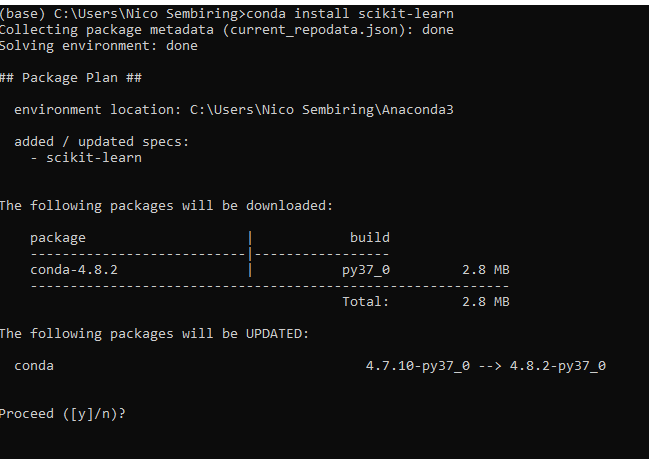
\includegraphics[width=4cm]{figures/1174096/1/install1.PNG}
            \centering
            \caption{Instalasi Package Scikit Learn}
        \end{figure}
		\hfill\break
		Klasifikasi adalah pengelompokan data di mana data yang digunakan memiliki label atau kelas target. Sehingga algoritma untuk menyelesaikan masalah klasifikasi dikategorikan ke dalam pembelajaran terbimbing.
		\item Kemudian pilih Y
		\begin{figure}[H]
            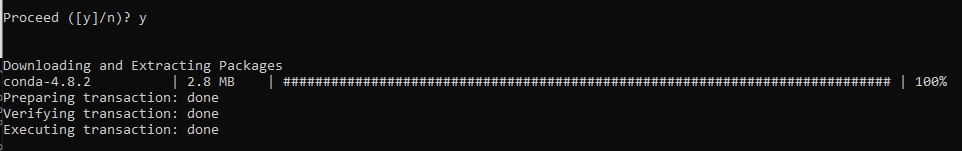
\includegraphics[width=4cm]{figures/1174096/1/install2.PNG}
            \centering
            \caption{pilih y}
        \end{figure}
	\end{itemize}
	
	\item Mencoba loading an example dataset
	\hfill\break
	\lstinputlisting[firstline=8, lastline=12]{src/1174096/1/1174096.py}
	\item Mencoba Learning dan predicting
	\hfill\break
	\lstinputlisting[firstline=14, lastline=24]{src/1174096/1/1174096.py}
	\item Mencoba Model Persistence
	\hfill\break
	\lstinputlisting[firstline=26, lastline=36]{src/1174096/1/1174096.py}
	\item Mencoba Conventions
	\hfill\break
	\lstinputlisting[firstline=38, lastline=56]{src/1174096/1/1174096.py}
\end{enumerate}
\subsection{Penanganan Error}
\begin{enumerate}
	\item ScreenShoot Error
	\begin{figure}[H]
		\includegraphics[width=4cm]{figures/1174096/error/1_import.png}
		\centering
		\caption{Import Error}
	\end{figure}
	\begin{figure}[H]
		\includegraphics[width=4cm]{figures/1174096/error/1_value.png}
		\centering
		\caption{Value Error}
	\end{figure}
	\item Tuliskan Kode Error dan Jenis Error
	\begin{itemize}
		\item Import Error
		\item Value Error
	\end{itemize}
	\item Cara Penangan Error
	\begin{itemize}
		\item Import Error
		\hfill\break
		Dengan Menginstall Library Yang Tidak Ditemukan
		\item Value Error
		\hfill\break
		Mengubah Bentuk Arraynya, Menjadi 1 Dimensi
	\end{itemize}
\end{enumerate}
\subsection{Bukti Tidak Plagiat}
\begin{figure}[H]
	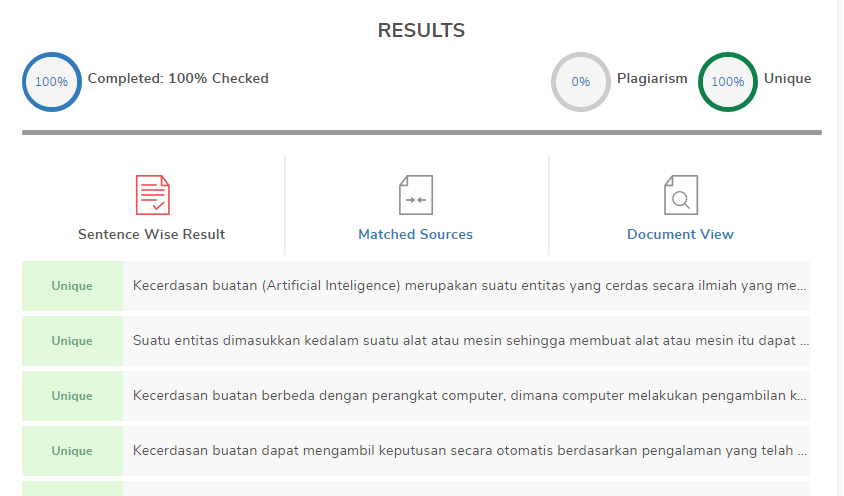
\includegraphics[width=4cm]{figures/1174096/bukti/plagiarisme.PNG}
	\centering
	\caption{Bukti Tidak Plagiarisme}
\end{figure}
%\section{1174012 - Damara Benedikta }
\subsection{Teori}
\begin{enumerate}
	\item Sejarah dan Perkembangan
	\hfill\break
	Kecerdasan Buatan atau dalam Bahasa inggris sering disebut Artifical Intelligence yang sering disebut juga sebagai AI, pada 10 tahun lalu masyarakat belum terlalu mengetahui hal tersebut dan masih menjadi bahan candaan dikalangan masyarakat. Awal perkembangan AI dimulai pada tahun 1952-1969 yang dimulai dengan kesuksesan Newwll dan temannya simon menggunakan sebuah program yang disebut dengan General Problem Solver. Program ini dibangun untuk tujuan penyelesaiin masalah secara manusiawi. Pada tahun 1966-1974 perkembangan kecerdasan buatan mulai melambat. Ada 3 faktor utama yang menyebabkan hal itu terjadi:
	\begin{itemize}
		\item Banyak subjek pada program AI yang bermunculan hanya mengandung sedikit atau bahkan sama sekali tidak  mengandung sama sekali pengetahuan (knowledge).
		\item Kecerdasan buatan harus bisa menyelesaikan banyak masalah.
		\item Untuk menghasilkan perilkau intelijensia ada beberapa batasan pada struktur yang bisa digunakan.
	\end{itemize}
	Definisi AI (Artificial Intelligence) atau kecerdasan buatan merupakan sebuah kecerdasan yang ditambahkan kepada sebuah system yang dapat diatur. Atau juga dapat didefinisikan kemampuan sebuah system untuk dapat menafsirkan data dengan benar untuk dapat mencapai sebuah tujuan dan tugas tertentu sehingga mesin dapat bekerja secara fleksibel seperti manusia.
	\item Definisi
	\hfill\break
	Supervised learning, klasifikasi, regresi, unsupervised learning, dataset, trainingset dan testingset.
	\begin{itemize}
		\item Supervised Learning
		\hfill\break
		Supervised Learning merupakan sebuah tipe learning yang mempunyai variable input dan variable output, tipe ini juga menggunakan satu algoritma atau lebih dari satu algoritma yang digunakan untuk mempelajari fungsi  pemetaan dari input ke output.
		\item Klasifikasi
		\hfill\break
		Klasifikasi adalah pengelompokan data di mana data yang digunakan memiliki label atau kelas target. Sehingga algoritma untuk menyelesaikan masalah klasifikasi dikategorikan ke dalam pembelajaran terbimbing.
		\item Regresi
		\hfill\break
		regressi metode analisis statistik yang digunakan untuk dapat melihat efek antara dua atau lebih variabel. Hubungan variabel dalam pertanyaan adalah fungsional yang diwujudkan dalam bentuk model matematika. Dalam analisis regresi, variabel dibagi menjadi dua jenis, yaitu variabel respons atau yang biasa disebut variabel dependen dan variabel independen atau dikenal sebagai variabel independen. Ada beberapa jenis analisis regresi, yaitu regresi sederhana yang mencakup linear sederhana dan regresi non-linear sederhana dan regresi berganda yang mencakup banyak linier atau non-linear berganda. Analisis regresi digunakan dalam pembelajaran mesin pembelajaran dengan metode pembelajaran terawasi.
		\item Unsupervised learning 
		\hfill\break
		unsupervised learning jenis pembelajaran di mana kita hanya memiliki data input (input data) tetapi tidak ada variabel output yang terkait. Tujuan dari pembelajaran tanpa pengawasan adalah untuk memodelkan struktur dasar atau distribusi data dengan tujuan mempelajari data lebih lanjut, dengan kata lain, itu adalah fungsi simpulan yang menggambarkan atau menjelaskan data.
		\item Data set
		\hfill\break
		Data set objek yang merepresentasikan data dan relasinya di memory. Strukturnya mirip dengan data di database. Dataset berisi koleksi dari datatable dan datarelation.
		\item Training Set
		\hfill\break
		Training set merupakan bagian dari dataset yang di latih untuk membuat prediksi atau menjalankan fungsi dari algoritma ML lain sesuai dengan masing-masing. Memberikan instruksi melalui algoritma sehingga mesin yang di praktikkan dapat menemukan korelasinya sendiri.
		\item Testing Set
		\hfill\break
		testing set adalah bagian dari dataset yang kami uji untuk melihat akurasinya, atau dengan kata lain untuk melihat kinerjanya.
	\end{itemize}
\end{enumerate}
\subsection{Praktek}
\begin{enumerate}
	\item Instalasi Library scikit dari ianaconda, mencoba kompilasi dan uji coba ambil contoh kode dan lihat variabel explorer
	\hfill\break
	\begin{figure}[H]
		
\includegraphics[width=4cm]{figures/1174012/1/ins1.PNG}
		\centering
		\caption{Instalasi Package Scikit Learn}
	\end{figure}
    \begin{figure}[H]
		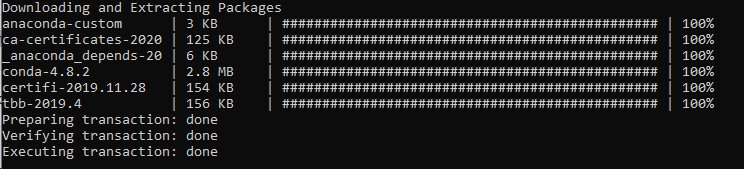
\includegraphics[width=4cm]{figures/1174012/1/ins2.PNG}
		\centering
		\caption{Instalasi Package Scikit Learn}
	\end{figure}
	\begin{figure}[H]
		\includegraphics[width=4cm]{figures/1174012/1/variabel.png}
		\centering
		\caption{Isi Variabel Explorer}
	\end{figure}
	\item Mencoba loading an example dataset
	\hfill\break
	\lstinputlisting[firstline=1, lastline=5]{src/1174012/1/1174012.py}
	\item Mencoba Learning dan predicting
	\hfill\break
	\lstinputlisting[firstline=7, lastline=18]{src/1174012/1/1174012.py}
	\item Mencoba Model Persistence
	\hfill\break
	\lstinputlisting[firstline=19, lastline=25]{src/1174012/1/1174012.py}
	\item Mencoba Conventions
	\hfill\break
	\lstinputlisting[firstline=31, lastline=43]{src/1174012/1/1174012.py}
\end{enumerate}
\subsection{Penanganan Error}
\begin{enumerate}
	\item ScreenShoot Error
	\begin{figure}[H]
		\includegraphics[width=4cm]{figures/1174012/error/1.png}
		\centering
		\caption{Import Error}
	\end{figure}
	\begin{figure}[H]
		\includegraphics[width=4cm]{figures/1174012/error/2.png}
		\centering
		\caption{Value Error}
	\end{figure}
	\item Tuliskan Kode Error dan Jenis Error
	\begin{itemize}
		\item Import Error
		\item Value Error
	\end{itemize}
	\item Cara Penangan Error
	\begin{itemize}
		\item Import Error
		\hfill\break
		Dengan Menginstall Library Yang Tidak Ditemukan
		\item Value Error
		\hfill\break
		Mengubah Bentuk Arraynya, Menjadi 1 Dimensi
	\end{itemize}
\end{enumerate}
\subsection{Bukti Tidak Plagiat}
\begin{figure}[H]
	\includegraphics[width=4cm]{figures/1174012/plagiat/plagiat.PNG}
	\centering
	\caption{Bukti Tidak Melakukan Plagiat Chapter 1}
\end{figure}
%\section{1174095 - Muhammad Dzihan Al-Bannai}
\subsection{Teori}
\begin{enumerate}

	\item Defenisi Kecerdasan Buatan
	\hfill\break
	Kecerdasan buatan yang jika dalam bahasa inggris ialah Artificial Intelligence (AI) adalah bagian dari ilmu komputer. Dengan penelitian dan pengembangan kecerdasan buatan, ia berusaha untuk tidak hanya berhasil tetapi untuk melengkapi pemikiran manusia dengan program komputer belajar mandiri. AI juga sudah banyak di aplikasikan di dunia bisnis, misalnya, dalam Google Maps. dan Istilah dalam AI juga sudah tidak asing lagi yaitu "Neural Network" dan "Deep learning" yang terkait dengan pengembangan kecerdasan buatan.



	\item Sejarah dan Perkembangan
	\hfill\break
	Pada tahun 1950 yang bertempat di AS kecerdasan buatan atau AI itu dimulai pada konferensi ilmiah di Dartmouth, M. Minsky, J.McCarthy, A. Newell, dan HA Simon adalah yang pertama berbicara tentang "kecerdasan buatan." Definisi yang sering dikutip untuk kecerdasan buatan diberikan oleh salah satu pendiri subjek, Marvin Minsky, pada tahun 1966: "Kecerdasan Buatan adalah ilmu membuat mesin melakukan hal-hal yang membutuhkan kecerdasan jika dilakukan oleh manusia." Jadi, ditentukan bahwa kecerdasan buatan adalah ilmu dan kedua mesin dapat mengambil alih pekerjaan manusia yang membutuhkan kecerdasan manusia. Adapun mengapa AI yaitu untuk pemecah an masalah umum dari para peneliti Newell, Shaw, dan Simon pada tahun 1960-an. Penelitian ini dapat memecahkan masalah sederhana. Namun, hasil penelitian tersebut tidak dapat digeneralisasi. Pada akhir 1960-an, program lain ditulis dengan ELIZA. Dengan demikian, Joseph Weizenbaum, seorang peneliti MIT,simulasikan sesi terapi. Pada tahun-tahun berikutnya, sains muda terus dikembangkan, yang diproduksi oleh MYCIN pada awal 1970-an dalam sistem inovatif lain berbasis AI. MYCIN dapat membantu dokter mendiagnosis.
	

	\item Kecerdasan buatan terbagi atas beberapa metode yaitu:
	\hfill\break
	Supervised learning, Unsupervised Learning, Klasifikasi, Regresi, Dataset, Trainingset dan juga Testingset.
	\begin{itemize}
		\item Supervised Learning
		\hfill\break
		Sebuah algoritma pembelajaran mesin yang dapat menerapkan informasi yang sudah ada dalam data dengan memberikan label tertentu, misalnya data yang telah diklasifikasikan sebelumnya (diarahkan). Algoritma ini mampu memberikan target untuk output yang dilakukan dengan membandingkan pengalaman belajar masa yang sudah lampau.
		\item Unsupervised Learning 
		\hfill\break
		Berbeda dengan Supervised Learning, Unsupervised Learning ialah sebuah pembelajaran mesin tanpa pengawasan adalah pembelajaran mesin yang digunakan pada data yang tidak memiliki informasi yang dapat diterapkan secara langsung (tidak diarahkan). Algoritma ini diharapkan dapat menemukan struktur tersembunyi dalam data yang tidak berlabel.
		\item Klasifikasi
		\hfill\break
		Klasifikasi adalah sampel milik dua kelas atau lebih dan ingin belajar dari data yang sudah diberi label cara memprediksi kelas data yang tidak berlabel. Contoh masalah klasifikasi adalah pengenalan digit tulisan tangan, di mana tujuannya adalah untuk menetapkan masing-masing vektor input ke salah satu dari sejumlah kategori diskrit. 
		\item Regresi
		\hfill\break
		Regrasi ialah sebuah metode untuk mengembangkan model (persamaan) yang menjelaskan hubungan antara beberapa variabel. Output dari analisis regresi adalah persamaan regresi. Dalam model regresi variabel dibagi menjadi dua bagian, yaitu variabel respon atau yang biasa juga disebut variabel dependen dan variabel explanatory atau juga biasa disebut variabel prediktor atau disebut juga variabel independen.
		\item Data set
		\hfill\break
		Dataset adalah sebuah kumpulan data atau objek dan bagaimana relasi dalam memori. Struktur Dataset mirip dengan data di dalam database. Dataset berisi koleksi dari datatable maupun data relasi.
		\item Training Set
		\hfill\break
		Training set ialah bagian dari dataset yang berfungsi untuk membuat prediksi atau mengatur fungsi dari algoritma-algoritma yang ada. Fungsi nya yang lain juga ada sesuai tujuannya masing-masing. Trainingset memberikan instruksi melalui algoritma sehingga mesin dapat mengerti dan membuat kolerasi sendiri.		
		\item Testing Set
		\hfill\break
		Sama seperti training set, testing set juga bagian dari dataset yang berfungsi menguji untuk melihat akurasinya, atau bisa juga untuk melihat suatu kinerja atau performa.
	\end{itemize}
\end{enumerate}
\subsection{Praktek}
\begin{enumerate}
	\item Instalasi Library scikit dari Anaconda, mencoba kompilasi dan uji coba ambil contoh kode dan lihat variabel explorer
	\hfill\break
	\begin{figure}[H]
		\includegraphics[width=4cm]{figures/1174095/tugas1/materi/1.PNG}
		\centering
		\caption{Instalasi Library Scikit Learn}
	\end{figure}
	\begin{figure}[H]
		\includegraphics[width=4cm]{figures/1174095/tugas1/materi/2.PNG}
		\centering
		\caption{Isi Variabel Explorer}
	\end{figure}
	\item Uji coba loading an example dataset
	\hfill\break
	\lstinputlisting[firstline=10, lastline=14]{src/1174095/tugas1.py}
	\item Uji coba Learning dan predicting
	\hfill\break
	\lstinputlisting[firstline=18, lastline=21]{src/1174095/tugas1.py}
	\item Uji coba Model Persistence
	\hfill\break
	\lstinputlisting[firstline=25, lastline=41]{src/1174095/tugas1.py}
	\item Uji coba Conventions
	\hfill\break
	\lstinputlisting[firstline=44, lastline=56]{src/1174095/tugas1.py}
\end{enumerate}
\subsection{Penanganan Error}
\begin{enumerate}
	\item ScreenShoot Error
	\begin{figure}[H]
		\includegraphics[width=4cm]{figures/1174095/tugas1/error/1.PNG}
		\centering
		\caption{Import Error}
	\end{figure}
	\begin{figure}[H]
		\includegraphics[width=4cm]{figures/1174095/tugas1/error/2.PNG}
		\centering
		\caption{FileNotFoundError}
	\end{figure}
	\item Tuliskan Kode Error dan Jenis Error
	\begin{itemize}
		\item Import Error
		\item FileNotFoundError
	\end{itemize}
	\item Cara Penangan Error
	\begin{itemize}
		\item Import Error
		\hfill\break
		Kesalahan pemanggilan pada import dapat menghasilkan error, seperti pada pemanggilan datasets, pastikan kembali pemanggilannya sesuai.
		\item FileNotFoundError
		\hfill\break
		Perhatikan format file pada joblib, format harus memakai titik terlebih dahulu.
	\end{itemize}
\end{enumerate}
\subsection{Bukti Tidak Plagiat}
\begin{figure}[H]
	\includegraphics[width=4cm]{figures/1174095/tugas1/buktiplagiat/plag.PNG}
	\centering
	\caption{Bukti Tidak Melakukan Plagiat Chapter 1}
\end{figure}
%\section{1174009 - Dwi Yulianingsih}
\subsection{Teori}
\begin{enumerate}
	\item Sejarah dan Perkembangan
	\hfill\break
	Kecerdasan Buatan atau dalam Bahasa inggris sering disebut Artifical Intelligence yang sering disebut juga sebagai AI, pada 10 tahun lalu masyarakat belum terlalu mengetahui hal tersebut dan masih menjadi bahan candaan dikalangan masyarakat. Awal perkembangan AI dimulai pada tahun 1952-1969 yang dimulai dengan kesuksesan Newwll dan temannya simon menggunakan sebuah program yang disebut dengan General Problem Solver. Program ini dibangun untuk tujuan penyelesaiin masalah secara manusiawi. Pada tahun 1966-1974 perkembangan kecerdasan buatan mulai melambat. Ada 3 faktor utama yang menyebabkan hal itu terjadi:
	\begin{itemize}
		\item Banyak subjek pada program AI yang bermunculan hanya mengandung sedikit atau bahkan sama sekali tidak  mengandung sama sekali pengetahuan (knowledge).
		\item Kecerdasan buatan harus bisa menyelesaikan banyak masalah.
		\item Untuk menghasilkan perilkau intelijensia ada beberapa batasan pada struktur yang bisa digunakan.
	\end{itemize}
	Definisi kecerdasan buatan itu sendiri adalah suatu system teknologi yang didalamnya ditambahakan kecerdasan oleh manusia, kecerdasan buatan diatur dan dikembangkan dalam konteks ilmiah, dan bentukan dari kecerdasan entitas ilmiah yang ada.
	\item Definisi
	\hfill\break
	Supervised learning, klasifikasi, regresi, unsupervised learning, dataset, trainingset dan testingset.
	\begin{itemize}
		\item Supervised Learning
		\hfill\break
		Supervised Learning merupakan sebuah tipe learning yang mempunyai variable input dan variable output, tipe ini juga menggunakan satu algoritma atau lebih dari satu algoritma yang digunakan untuk mempelajari fungsi  pemetaan dari input ke output.
		\item Klasifikasi
		\hfill\break
		Klasifikasi adalah pengelompokan data di mana data yang digunakan memiliki label atau kelas target. Sehingga algoritma untuk menyelesaikan masalah klasifikasi dikategorikan ke dalam pembelajaran terbimbing.
		\item Regresi
		\hfill\break
		regressi metode analisis statistik yang digunakan untuk dapat melihat efek antara dua atau lebih variabel. Hubungan variabel dalam pertanyaan adalah fungsional yang diwujudkan dalam bentuk model matematika. Dalam analisis regresi, variabel dibagi menjadi dua jenis, yaitu variabel respons atau yang biasa disebut variabel dependen dan variabel independen atau dikenal sebagai variabel independen. Ada beberapa jenis analisis regresi, yaitu regresi sederhana yang mencakup linear sederhana dan regresi non-linear sederhana dan regresi berganda yang mencakup banyak linier atau non-linear berganda. Analisis regresi digunakan dalam pembelajaran mesin pembelajaran dengan metode pembelajaran terawasi.
		\item Unsupervised learning 
		\hfill\break
		unsupervised learning jenis pembelajaran di mana kita hanya memiliki data input (input data) tetapi tidak ada variabel output yang terkait. Tujuan dari pembelajaran tanpa pengawasan adalah untuk memodelkan struktur dasar atau distribusi data dengan tujuan mempelajari data lebih lanjut, dengan kata lain, itu adalah fungsi simpulan yang menggambarkan atau menjelaskan data.
		\item Data set
		\hfill\break
		Data set objek yang merepresentasikan data dan relasinya di memory. Strukturnya mirip dengan data di database. Dataset berisi koleksi dari datatable dan datarelation.
		\item Training Set
		\hfill\break
		Training set adalah bagian dari dataset yang di latih untuk membuat prediksi atau menjalankan fungsi dari algoritma ML lain sesuai dengan masing-masing. Memberikan instruksi melalui algoritma sehingga mesin yang di praktikkan dapat menemukan korelasinya sendiri.
		\item Testing Set
		\hfill\break
		testing set adalah bagian dari dataset yang kami uji untuk melihat akurasinya, atau dengan kata lain untuk melihat kinerjanya.
	\end{itemize}
\end{enumerate}
\subsection{Praktek}
\begin{enumerate}
	\item Instalasi Library scikit dari ianaconda, mencoba kompilasi dan uji coba ambil contoh kode dan lihat variabel explorer
	\hfill\break
	\begin{figure}[H]
		\includegraphics[width=4cm]{figures/1174009/materi/1.png}
		\centering
		\caption{Instalasi Package Scikit Learn}
	\end{figure}
	\begin{figure}[H]
		\includegraphics[width=4cm]{figures/1174009/materi/2.PNG}
		\centering
		\caption{Isi Variabel Explorer}
	\end{figure}
	\item Mencoba loading an example dataset
	\hfill\break
	\lstinputlisting[firstline=7, lastline=11]{src/1174009/tugas1.py}
	\item Mencoba Learning dan predicting
	\hfill\break
	\lstinputlisting[firstline=13, lastline=22]{src/1174009/tugas1.py}
	\item Mencoba Model Persistence
	\hfill\break
	\lstinputlisting[firstline=25, lastline=34]{src/1174009/tugas1.py}
	\item Mencoba Conventions
	\hfill\break
	\lstinputlisting[firstline=37, lastline=48]{src/1174009/tugas1.py}
\end{enumerate}
\subsection{Penanganan Error}
\begin{enumerate}
	\item ScreenShoot Error
	\begin{figure}[H]
		\includegraphics[width=4cm]{figures/1174009/error/3.PNG}
		\centering
		\caption{Import Error}
	\end{figure}
	\begin{figure}[H]
		\includegraphics[width=4cm]{figures/1174009/error/4.PNG}
		\centering
		\caption{Value Error}
	\end{figure}
	\item Tuliskan Kode Error dan Jenis Error
	\begin{itemize}
		\item Import Error
		\item Value Error
	\end{itemize}
	\item Cara Penangan Error
	\begin{itemize}
		\item Import Error
		\hfill\break
		Dengan Menginstall Library Yang Tidak Ditemukan
		\item Value Error
		\hfill\break
		Mengubah Bentuk Arraynya, Menjadi 1 Dimensi
	\end{itemize}
\end{enumerate}
\subsection{Bukti Tidak Plagiat}
\begin{figure}[H]
	\includegraphics[width=4cm]{figures/1174009/buktiplagiat/1.png}
	\centering
	\caption{Bukti Tidak Melakukan Plagiat Chapter 1}
\end{figure}
%\section{1174008 - Arjun Yuda Firwanda}
\subsection{Teori}
\begin{enumerate}
	\item Definisi Kecerdasan Buatan
	\hfill\break
	Definisi Kecerdasan Buatan (Artificial Intelligence) yakni sebagai kecerdasan entitas ilmiah. Kecerdasan Buatan diciptakan dalam suatu mesin komputer agar dapat melakukan pekerjaan seperti halnya yang dilakukan manusia.
	
	\item Sejarah dan Perkembangan Kecerdasan Buatan
	\hfill\break
	Sejarah dan Kecerdasan Buatan tidak lepas dari sosok John McCarthy. Ia sebagai "Bapak AI".

	\begin{itemize}
		\item Cikal bakal kecerdasan buatan (tahun 1943 - 1955)
		
		\item Kelahiran Kecerdasan Buatan (tahun 1956)
		
		\item Awal kecerdasan buatan merupakan tahap pengembangan aplikasi AI yang sukses dibandingkan dengan program komputer (tahun 1952 - 1969)
		
		\item Kecerdasan Buatan menjadi industry  (tahun 1980 - sekarang)
		
		\item Kecerdasan Buatan menjadi disiplin ilmu (tahun 1987 - sekarang)
		
		\item Kecerdasan Buatan menampakkan diri di semua bidang (tahun 1995 - sekarang)

	\end{itemize}

	\item Definisi Supervised Learning
	\hfill\break
	Supervised Learning merupakan pembelajaran yang ada supervisornya. Maksudnya adalah label di tiap data nya. Label maksudnya merupakan sebuatan tag dari data yang ditambahkan dalam machine learning model.
	
	\item Regresi
	\hfill\break
	Regresi merupakan menebak nilai output dari nilai input yang diberikan, berdasarkan pola input - ouput sebelumnya.

	\item Klasifikasi
	\hfill\break
	Klasifikasi, merupakan mengetahui jenis kelamin siswa dari tinggi dan berat badannya.

	\item Definisi Unsupervised Learning
	\hfill\break
	Unsupervised learning memiliki keunggulan. Jika unsupervised learning memiliki label sebagai dasar prediksi baik serta membuat clasification dan regression algorithm K-Means, Hierarchical Clustering, DBSCAN, Fuzzy C-Means, Self-Organizing Map.

	\item Data Set
	\hfill\break
	Data Set, merupakan objek yang merepresentasikan data dan relasinya. Strukturnya mirip dengan data di database. Dataset berisi koleksi dari datatable dan datarelation.

	\item Trainning Set
	\hfill\break
	Trainning Set, merupakan konteks machine learning Training = latihan.

	\item Testing Set
	\hfill\break
	Testing Set, merupakan melakukan evaluasi terhadap performa algoritma tersebut. Pada proses testing ini, dilakukan untuk mwengetahui performa algoritma akan diuji menggunakan testing set, dimana testing set dan training set merupakan data yang berbeda.

\end{enumerate}


\subsection{Praktek}
\begin{enumerate}
	\item Instalasi Library scikit dari ianaconda, mencoba kompilasi dan uji coba ambil contoh kode dan lihat variabel explorer
	\hfill\break
	\begin{figure}[H]
		\includegraphics[width=4cm]{figures/1174008/1/instalasi.PNG}
		\centering
		\caption{Instalasi Package Scikit Learn}
	\end{figure}
	\begin{figure}[H]
		\includegraphics[width=4cm]{figures/1174008/1/variable.PNG}
		\centering
		\caption{Isi Variabel Explorer}
	\end{figure}

	\item Mencoba loading an example dataset
	\hfill\break
	\lstinputlisting[firstline=7, lastline=11]{src/1174008/1/1174008.py}

	\item Mencoba Learning dan predicting
	\hfill\break
	\lstinputlisting[firstline=13, lastline=22]{src/1174008/1/1174008.py}

	\item Mencoba Model Persistence
	\hfill\break
	\lstinputlisting[firstline=25, lastline=34]{src/1174008/1/1174008.py}

	\item Mencoba Conventions
	\hfill\break
	\lstinputlisting[firstline=37, lastline=48]{src/1174008/1/1174008.py}
\end{enumerate}

\subsection{Penanganan Error}
\begin{enumerate}
	\item ScreenShoot Error
	\begin{figure}[H]
		\includegraphics[width=4cm]{figures/1174008/error/error.PNG}
		\centering
		\caption{ Error Joblib}
	\end{figure}

	\item Tuliskan Kode Error dan Jenis Error
	\begin{itemize}
		\item Import Error
		\item Value Error
	\end{itemize}

	\item Cara Penangan Error
	\begin{itemize}
		\item Import Error
		\hfill\break
		Dengan Menginstall Library Yang Tidak Ditemukan
		\item Value Error
		\hfill\break
		Mengubah Bentuk Arraynya, Menjadi 1 Dimensi
	\end{itemize}
\end{enumerate}

\subsection{Bukti Tidak Plagiat}
\begin{figure}[H]
	\includegraphics[width=4cm]{figures/1174008/bukti/CekPlagiarisme.PNG}
	\centering
	\caption{Bukti Tidak Melakukan Plagiat Chapter 1}
\end{figure}
%\section{1174005 - Oniwaldus Bere Mali}
\subsection{Teori}
\begin{enumerate}

\item Sejarah dan Perkembangan
	\hfill\break
	Definisi kecerdasan buatan (AI) Kecerdasan buatan (Bahasa Inggris: kecerdasan buatan atau AI) didefinisikan sebagai kecerdasan entitas ilmiah. Sistem ini umumnya dianggap komputer. Kecerdasan dibuat dan ditempatkan di sebuah mesin (komputer) sehingga dapat berfungsi seperti manusia. Berbagai jenis bidang yang menggunakan kecerdasan buatan meliputi sistem pakar, permainan komputer (game), logika fuzzy, jaringan saraf tiruan, dan robotika. Banyak hal yang tampaknya sulit bagi kecerdasan manusia, tetapi bagi ilmu komputer, relatif tidak bermasalah. Misalnya: mengubah persamaan, memecahkan persamaan integral, melakukan catur atau backgammon. Di sisi lain, hal-hal yang tampaknya membutuhkan sedikit kecerdasan bagi orang masih sulit untuk diproses dalam pengolahan data. Misalnya: 1. kecerdasan: kemampuan untuk memperoleh dan menggunakan pengetahuan 2. atau kecerdasan yang diukur dengan tes kecerdasan. KONSEP DASAR KECERDASAN ARTIFICIAL INTELLIGENCE (AI) Kecerdasan buatan dapat didefinisikan sebagai cabang ilmu komputer yang mempelajari otomatisasi perilaku cerdas (intelligent). Kecerdasan buatan dapat membuat komputer berpikir. Kecerdasan buatan dapat meniru proses pembelajaran manusia sehingga informasi baru dapat diserap dan digunakan sebagai referensi untuk masa depan. Asumsi dasar: hipotesis yang berkaitan dengan sistem simbol fisik (PSSH): proses pemrosesan informasi dapat dianggap sebagai pemrosesan atau manipulasi simbol, di mana informasi. 2. dilambangkan dengan simbol. Hipotesis-hipotesis ini memunculkan apa yang disebut elaborasi simbolis (ditemukan oleh Newell dan Simon). Perbedaan antara kecerdasan buatan (komputer) dan kecerdasan alami (manusia): Kecerdasan buatan: · permanen · mudah diduplikasi dan disebarkan · bisa lebih murah daripada orang cerdas · konsisten dan lengkap · dapat didokumentasikan Kecerdasan alami: · Jadilah kreatif · 
	
	\item Kecerdasan buatan terbagi atas beberapa metode yaitu:
	\hfill\break
	Supervised learning, Unsupervised Learning, Klasifikasi, Regresi, Dataset, Trainingset dan juga Testingset.
	\begin{itemize}
		\item Supervised Learning
		\hfill\break
		Sebuah algoritma pembelajaran mesin yang dapat menerapkan informasi yang sudah ada dalam data dengan memberikan label tertentu, misalnya data yang telah diklasifikasikan sebelumnya (diarahkan). Algoritma ini mampu memberikan target untuk output yang dilakukan dengan membandingkan pengalaman belajar masa yang sudah lampau.
		\item Unsupervised Learning 
		\hfill\break
		Berbeda dengan Supervised Learning, Unsupervised Learning ialah sebuah pembelajaran mesin tanpa pengawasan adalah pembelajaran mesin yang digunakan pada data yang tidak memiliki informasi yang dapat diterapkan secara langsung (tidak diarahkan). Algoritma ini diharapkan dapat menemukan struktur tersembunyi dalam data yang tidak berlabel.
		\item Klasifikasi
		\hfill\break
		Klasifikasi adalah sampel milik dua kelas atau lebih dan ingin belajar dari data yang sudah diberi label cara memprediksi kelas data yang tidak berlabel. Contoh masalah klasifikasi adalah pengenalan digit tulisan tangan, di mana tujuannya adalah untuk menetapkan masing-masing vektor input ke salah satu dari sejumlah kategori diskrit. 
		\item Regresi
		\hfill\break
		Regrasi ialah sebuah metode untuk mengembangkan model (persamaan) yang menjelaskan hubungan antara beberapa variabel. Output dari analisis regresi adalah persamaan regresi. Dalam model regresi variabel dibagi menjadi dua bagian, yaitu variabel respon atau yang biasa juga disebut variabel dependen dan variabel explanatory atau juga biasa disebut variabel prediktor atau disebut juga variabel independen.
		\item Data set
		\hfill\break
		Dataset adalah sebuah kumpulan data atau objek dan bagaimana relasi dalam memori. Struktur Dataset mirip dengan data di dalam database. Dataset berisi koleksi dari datatable maupun data relasi.
		\item Training Set
		\hfill\break
		Training set ialah bagian dari dataset yang berfungsi untuk membuat prediksi atau mengatur fungsi dari algoritma-algoritma yang ada. Fungsi nya yang lain juga ada sesuai tujuannya masing-masing. Trainingset memberikan instruksi melalui algoritma sehingga mesin dapat mengerti dan membuat kolerasi sendiri.		
		\item Testing Set
		\hfill\break
		Sama seperti training set, testing set juga bagian dari dataset yang berfungsi menguji untuk melihat akurasinya, atau bisa juga untuk melihat suatu kinerja atau performa.
	\end{itemize}
\end{enumerate}
\end{enumerate}
\subsection{Praktek}
\begin{enumerate}
	\item Instalasi Library scikit dari Anaconda, mencoba kompilasi dan uji coba ambil contoh kode dan lihat variabel explorer
	\hfill\break
	\begin{figure}[H]
		\includegraphics[width=4cm]{figures/1174005/tugas1/materi/1.PNG}
		\centering
		\caption{Instalasi Library Scikit Learn}
	\end{figure}
	\begin{figure}[H]
		\includegraphics[width=4cm]{figures/1174005/tugas1/materi/2.PNG}
		\centering
		\caption{Isi Variabel Explorer}
	\end{figure}
	\item Uji coba loading an example dataset
	\hfill\break
	\lstinputlisting[firstline=7, lastline=12]{src/1174005/1174005.py}
	\item Uji coba Learning dan predicting
	\hfill\break
	\lstinputlisting[firstline=15, lastline=18]{src/1174005/1174005.py}
	\item Uji coba Model Persistence
	\hfill\break
	\lstinputlisting[firstline=21, lastline=37]{src/1174005/1174005.py}
	\item Uji coba Conventions
	\hfill\break
	\lstinputlisting[firstline=40, lastline=52]{src/1174005/1174005.py}
\end{enumerate}
\subsection{Penanganan Error}
\begin{enumerate}
	\item ScreenShoot Error
	\begin{figure}[H]
		\includegraphics[width=4cm]{figures/1174005/tugas1/error/3.PNG}
		\centering
		\caption{NameError: name 'digit' is not defined}
	\end{figure}
	\begin{figure}[H]
		\includegraphics[width=4cm]{figures/1174005/tugas1/error/4.PNG}
		\centering
		\caption{Import Error}
	\end{figure}
	\item Tuliskan Kode Error dan Jenis Error
	\begin{itemize}
		\item NameError: name 'digit' is not defined
		\item Import Error
	\end{itemize}
	\item Cara Penangan Error
	\begin{itemize}
		\item NameError: name 'digit' is not defined
		\hfill\break
		Error terdapat pada digit dan seharusnya digids
		\item Import Error
		\hfill\break
		Error terdapat typo pada dataset, seharusnya datasets
	\end{itemize}
\end{enumerate}
\subsection{Bukti Tidak Plagiat}
\begin{figure}[H]
	\includegraphics[width=4cm]{figures/1174005/tugas1/plagiat/5.PNG}
	\centering
	\caption{Bukti Tidak Melakukan Plagiat Chapter 1}
\end{figure}
%\section{1174026- Felix Setiawan Lase}
\subsection{Teori}
\begin{enumerate}
	\item Sejarah dan Perkembangan
	\hfill\break
	Kecerdasan Buatan atau dalam Bahasa inggris sering disebut Artifical Intelligence yang sering disebut juga sebagai AI, pada 10 tahun lalu masyarakat belum terlalu mengetahui hal tersebut dan masih menjadi bahan candaan dikalangan masyarakat. Awal perkembangan AI dimulai pada tahun 1952-1969 yang dimulai dengan kesuksesan Newwll dan temannya simon menggunakan sebuah program yang disebut dengan General Problem Solver. Program ini dibangun untuk tujuan penyelesaiin masalah secara manusiawi. Pada tahun 1966-1974 perkembangan kecerdasan buatan mulai melambat. Ada 3 faktor utama yang menyebabkan hal itu terjadi:
	\begin{itemize}
		\item Banyak subjek pada program AI yang bermunculan hanya mengandung sedikit atau bahkan sama sekali tidak  mengandung sama sekali pengetahuan (knowledge).
		\item Kecerdasan buatan harus bisa menyelesaikan banyak masalah.
		\item Untuk menghasilkan perilkau intelijensia ada beberapa batasan pada struktur yang bisa digunakan.
	\end{itemize}
	Definisi kecerdasan buatan itu sendiri adalah suatu system teknologi yang didalamnya ditambahakan kecerdasan oleh manusia, kecerdasan buatan diatur dan dikembangkan dalam konteks ilmiah, dan bentukan dari kecerdasan entitas ilmiah yang ada.
	\item Definisi
	\hfill\break
	Supervised learning, klasifikasi, regresi, unsupervised learning, dataset, trainingset dan testingset.
	\begin{itemize}
		\item Supervised Learning
		\hfill\break
		Supervised Learning merupakan sebuah tipe learning yang mempunyai variable input dan variable output, tipe ini juga menggunakan satu algoritma atau lebih dari satu algoritma yang digunakan untuk mempelajari fungsi  pemetaan dari input ke output.
		\item Klasifikasi
		\hfill\break
		Klasifikasi adalah pengelompokan data di mana data yang digunakan memiliki label atau kelas target. Sehingga algoritma untuk menyelesaikan masalah klasifikasi dikategorikan ke dalam pembelajaran terbimbing.
		\item Regresi
		\hfill\break
		regressi metode analisis statistik yang digunakan untuk dapat melihat efek antara dua atau lebih variabel. Hubungan variabel dalam pertanyaan adalah fungsional yang diwujudkan dalam bentuk model matematika. Dalam analisis regresi, variabel dibagi menjadi dua jenis, yaitu variabel respons atau yang biasa disebut variabel dependen dan variabel independen atau dikenal sebagai variabel independen. Ada beberapa jenis analisis regresi, yaitu regresi sederhana yang mencakup linear sederhana dan regresi non-linear sederhana dan regresi berganda yang mencakup banyak linier atau non-linear berganda. Analisis regresi digunakan dalam pembelajaran mesin pembelajaran dengan metode pembelajaran terawasi.
		\item Unsupervised learning 
		\hfill\break
		unsupervised learning jenis pembelajaran di mana kita hanya memiliki data input (input data) tetapi tidak ada variabel output yang terkait. Tujuan dari pembelajaran tanpa pengawasan adalah untuk memodelkan struktur dasar atau distribusi data dengan tujuan mempelajari data lebih lanjut, dengan kata lain, itu adalah fungsi simpulan yang menggambarkan atau menjelaskan data.
		\item Data set
		\hfill\break
		Data set objek yang merepresentasikan data dan relasinya di memory. Strukturnya mirip dengan data di database. Dataset berisi koleksi dari datatable dan datarelation.
		\item Training Set
		\hfill\break
		Training set adalah bagian dari dataset yang di latih untuk membuat prediksi atau menjalankan fungsi dari algoritma ML lain sesuai dengan masing-masing. Memberikan instruksi melalui algoritma sehingga mesin yang di praktikkan dapat menemukan korelasinya sendiri.
		\item Testing Set
		\hfill\break
		testing set adalah bagian dari dataset yang kami uji untuk melihat akurasinya, atau dengan kata lain untuk melihat kinerjanya.
	\end{itemize}
\end{enumerate}
\subsection{Praktek}
\begin{enumerate}
	\item Instalasi Library scikit dari ianaconda, mencoba kompilasi dan uji coba ambil contoh kode dan lihat variabel explorer
	\hfill\break
	\begin{figure}[H]
		\includegraphics[width=4cm]{figures/1174026/1/install.PNG}
		\centering
		\caption{Instalasi Package Scikit Learn}
	\end{figure}
	\item Mencoba loading an example dataset
	\hfill\break
	\lstinputlisting[firstline=10, lastline=13]{src/1174026/1/1174026.py}
	\item Mencoba Learning dan predicting
	\hfill\break
	\lstinputlisting[firstline=17, lastline=26]{src/1174026/1/1174026.py}
	\item Mencoba Model Persistence
	\hfill\break
	\lstinputlisting[firstline=30, lastline=39]{src/1174026/1/1174026.py}
	\item Mencoba Conventions
	\hfill\break
	\lstinputlisting[firstline=42, lastline=54]{src/1174026/1/1174026.py}
\end{enumerate}
\subsection{Penanganan Error}
\begin{enumerate}
	\item ScreenShoot Error
	\begin{figure}[H]
		\includegraphics[width=4cm]{figures/1174026/1/error.png}
		\centering
		\caption{Import Error}
	\end{figure}
	\item Tuliskan Kode Error dan Jenis Error
	\begin{itemize}
		\item Value Error
	\end{itemize}
	\item Cara Penangan Error
	\begin{itemize}
		\item Value Error
		\hfill\break
		Mengubah bentuk array jadi satu dimensi (a = a.reshape(1,-1)   
	\end{itemize}
\end{enumerate}
\subsection{Bukti Tidak Plagiat}
\begin{figure}[H]
	\includegraphics[width=4cm]{figures/1174026/1/plagiat.PNG}
	\centering
	\caption{Bukti Tidak Melakukan Plagiat }
\end{figure}
%\section{1174004 - Choirulanam}
\subsection{Teori}
\begin{enumerate}
	\item Sejarah dan Perkembangan
	\hfill\break
	Kecerdasan Buatan atau dalam Bahasa inggris sering disebut Artifical Intelligence yang sering disebut juga sebagai AI, pada 10 tahun lalu masyarakat belum terlalu mengetahui hal tersebut dan masih menjadi bahan candaan dikalangan masyarakat. Awal perkembangan AI dimulai pada tahun 1952-1969 yang dimulai dengan kesuksesan Newwll dan temannya simon menggunakan sebuah program yang disebut dengan General Problem Solver. Program ini dibangun untuk tujuan penyelesaiin masalah secara manusiawi. Pada tahun 1966-1974 perkembangan kecerdasan buatan mulai melambat. Ada 3 faktor utama yang menyebabkan hal itu terjadi:
	\begin{itemize}
		\item Banyak subjek pada program AI yang bermunculan hanya mengandung sedikit atau bahkan sama sekali tidak  mengandung sama sekali pengetahuan (knowledge).
		\item Kecerdasan buatan harus bisa menyelesaikan banyak masalah.
		\item Untuk menghasilkan perilkau intelijensia ada beberapa batasan pada struktur yang bisa digunakan.
	\end{itemize}
	Definisi kecerdasan buatan itu sendiri adalah suatu system teknologi yang didalamnya ditambahakan kecerdasan oleh manusia, kecerdasan buatan diatur dan dikembangkan dalam konteks ilmiah, dan bentukan dari kecerdasan entitas ilmiah yang ada.
	\item Definisi
	\hfill\break
	Supervised learning, klasifikasi, regresi, unsupervised learning, dataset, trainingset dan testingset.
	\begin{itemize}
		\item Supervised Learning
		\hfill\break
		Supervised Learning merupakan sebuah tipe learning yang mempunyai variable input dan variable output, tipe ini juga menggunakan satu algoritma atau lebih dari satu algoritma yang digunakan untuk mempelajari fungsi  pemetaan dari input ke output.
		\item Klasifikasi
		\hfill\break
		Klasifikasi adalah pengelompokan data di mana data yang digunakan memiliki label atau kelas target. Sehingga algoritma untuk menyelesaikan masalah klasifikasi dikategorikan ke dalam pembelajaran terbimbing.
		\item Regresi
		\hfill\break
		regressi metode analisis statistik yang digunakan untuk dapat melihat efek antara dua atau lebih variabel. Hubungan variabel dalam pertanyaan adalah fungsional yang diwujudkan dalam bentuk model matematika. Dalam analisis regresi, variabel dibagi menjadi dua jenis, yaitu variabel respons atau yang biasa disebut variabel dependen dan variabel independen atau dikenal sebagai variabel independen. Ada beberapa jenis analisis regresi, yaitu regresi sederhana yang mencakup linear sederhana dan regresi non-linear sederhana dan regresi berganda yang mencakup banyak linier atau non-linear berganda. Analisis regresi digunakan dalam pembelajaran mesin pembelajaran dengan metode pembelajaran terawasi.
		\item Unsupervised learning 
		\hfill\break
		unsupervised learning jenis pembelajaran di mana kita hanya memiliki data input (input data) tetapi tidak ada variabel output yang terkait. Tujuan dari pembelajaran tanpa pengawasan adalah untuk memodelkan struktur dasar atau distribusi data dengan tujuan mempelajari data lebih lanjut, dengan kata lain, itu adalah fungsi simpulan yang menggambarkan atau menjelaskan data.
		\item Data set
		\hfill\break
		Data set objek yang merepresentasikan data dan relasinya di memory. Strukturnya mirip dengan data di database. Dataset berisi koleksi dari datatable dan datarelation.
		\item Training Set
		\hfill\break
		Training set adalah bagian dari dataset yang di latih untuk membuat prediksi atau menjalankan fungsi dari algoritma ML lain sesuai dengan masing-masing. Memberikan instruksi melalui algoritma sehingga mesin yang di praktikkan dapat menemukan korelasinya sendiri.
		\item Testing Set
		\hfill\break
		testing set adalah bagian dari dataset yang kami uji untuk melihat akurasinya, atau dengan kata lain untuk melihat kinerjanya.
	\end{itemize}
\end{enumerate}
\subsection{Praktek}
\begin{enumerate}
	\item Instalasi Library scikit dari ianaconda, mencoba kompilasi dan uji coba ambil contoh kode dan lihat variabel explorer
	\hfill\break
	\begin{figure}[H]
		\includegraphics[width=4cm]{figures/1174004/1/instalasi.png}
		\centering
		\caption{Instalasi Package Scikit Learn}
	\end{figure}
	\begin{figure}[H]
		\includegraphics[width=4cm]{figures/1174004/1/variabel.png}
		\centering
		\caption{Isi Variabel Explorer}
	\end{figure}
	\item Mencoba loading an example dataset
	\hfill\break
	\lstinputlisting[firstline=7, lastline=11]{src/1174004/1/1174004.py}
	\item Mencoba Learning dan predicting
	\hfill\break
	\lstinputlisting[firstline=13, lastline=22]{src/1174004/1/1174004.py}
	\item Mencoba Model Persistence
	\hfill\break
	\lstinputlisting[firstline=25, lastline=34]{src/1174004/1/1174004.py}
	\item Mencoba Conventions
	\hfill\break
	\lstinputlisting[firstline=37, lastline=48]{src/1174004/1/1174004.py}
\end{enumerate}
\subsection{Penanganan Error}
\begin{enumerate}
	\item ScreenShoot Error
	\begin{figure}[H]
		\includegraphics[width=4cm]{figures/1174004/error/1_import.png}
		\centering
		\caption{Import Error}
	\end{figure}
	\begin{figure}[H]
		\includegraphics[width=4cm]{figures/1174004/error/1_value.png}
		\centering
		\caption{Value Error}
	\end{figure}
	\item Tuliskan Kode Error dan Jenis Error
	\begin{itemize}
		\item Import Error
		\item Value Error
	\end{itemize}
	\item Cara Penangan Error
	\begin{itemize}
		\item Import Error
		\hfill\break
		Dengan Menginstall Library Yang Tidak Ditemukan
		\item Value Error
		\hfill\break
		Mengubah Bentuk Arraynya, Menjadi 1 Dimensi
	\end{itemize}
\end{enumerate}
\subsection{Bukti Tidak Plagiat}
\begin{figure}[H]
	\includegraphics[width=4cm]{figures/1174004/bukti/1.png}
	\centering
	\caption{Bukti Tidak Melakukan Plagiat Chapter 1}
\end{figure}
%\section{1164013 - Ikrima Ningrumsari Mulyana}
\subsection{Teori}
\begin{enumerate}
	\item Sejarah dan Perkembangan
	\hfill\break
	Kecerdasan Buatan atau dalam Bahasa inggris sering disebut Artifical Intelligence yang sering disebut juga sebagai AI, pada 10 tahun lalu masyarakat belum terlalu mengetahui hal tersebut dan masih menjadi bahan candaan dikalangan masyarakat. Awal perkembangan AI dimulai pada tahun 1952-1969 yang dimulai dengan kesuksesan Newwll dan temannya simon menggunakan sebuah program yang disebut dengan General Problem Solver. Program ini dibangun untuk tujuan penyelesaiin masalah secara manusiawi. Pada tahun 1966-1974 perkembangan kecerdasan buatan mulai melambat. Ada 3 faktor utama yang menyebabkan hal itu terjadi:
	\begin{itemize}
		\item Banyak subjek pada program AI yang bermunculan hanya mengandung sedikit atau bahkan sama sekali tidak  mengandung sama sekali pengetahuan (knowledge).
		\item Kecerdasan buatan harus bisa menyelesaikan banyak masalah.
		\item Untuk menghasilkan perilkau intelijensia ada beberapa batasan pada struktur yang bisa digunakan.
	\end{itemize}
	Definisi Kecerdasan buatan adalah kecerdasan yang ditambahkan pada suatu sistem untuk menafsirkan data eksternal dengan benar dan belajar dari data tersebut untuk mencapai tujuan tertentu melalui adaptasi yang fleksibel.
	\item Definisi
	\hfill\break
	Supervised learning, klasifikasi, regresi, unsupervised learning, dataset, trainingset dan testingset.
	\begin{itemize}
		\item Supervised Learning
		\hfill\break
		Supervised Learning merupakan sebuah tipe learning yang mempunyai variable input dan variable output, tipe ini juga menggunakan satu algoritma atau lebih dari satu algoritma yang digunakan untuk mempelajari fungsi  pemetaan dari input ke output.
		\item Klasifikasi
		\hfill\break
		Klasifikasi adalah pengelompokan data di mana data yang digunakan memiliki label atau kelas target. Sehingga algoritma untuk menyelesaikan masalah klasifikasi dikategorikan ke dalam pembelajaran terbimbing.
		\item Regresi
		\hfill\break
		regressi metode analisis statistik yang digunakan untuk dapat melihat efek antara dua atau lebih variabel. Hubungan variabel dalam pertanyaan adalah fungsional yang di wujudkan dalam bentuk model matematika. Dalam analisis regresi, variabel dibagi menjadi dua jenis, yaitu variabel respons atau yang biasa disebut variabel dependen dan variabel independen atau dikenal sebagai variabel independen. Ada beberapa jenis analisis regresi, yaitu regresi sederhana yang mencakup linear sederhana dan regresi non-linear sederhana dan regresi berganda yang mencakup banyak linier atau non-linear berganda. Analisis regresi digunakan dalam pembelajaran mesin pembelajaran dengan metode pembelajaran terawasi.
		\item Unsupervised learning 
		\hfill\break
		unsupervised learning jenis pembelajaran di mana kita hanya memiliki data input (input data) tetapi tidak ada variabel output yang terkait. Tujuan dari pembelajaran tanpa pengawasan adalah untuk memodelkan struktur dasar atau distribusi data dengan tujuan mempelajari data lebih lanjut, dengan kata lain, itu adalah fungsi simpulan yang menggambarkan atau menjelaskan data.
		\item Data set
		\hfill\break
		Data set objek yang merepresentasikan data dan relasinya di memory. Strukturnya mirip dengan data di database. Dataset berisi koleksi dari datatable dan datarelation.
		\item Training Set
		\hfill\break
		Training set adalah bagian dari dataset yang di latih untuk membuat prediksi atau menjalankan fungsi dari algoritma ML lain sesuai dengan masing-masing. Memberikan instruksi melalui algoritma sehingga mesin yang di praktikkan dapat menemukan korelasinya sendiri.
		\item Testing Set
		\hfill\break
		testing set adalah bagian dari dataset yang kami uji untuk melihat akurasinya, atau dengan kata lain untuk melihat kinerjanya.
	\end{itemize}
\end{enumerate}
\subsection{Praktek}
\begin{enumerate}
	\item Instalasi Library scikit dari ianaconda, mencoba kompilasi dan uji coba ambil contoh kode dan lihat variabel explorer
	\hfill\break
	\begin{figure}[H]
		\includegraphics[width=4cm]{figures/1164013/1/sckt.png}
		\centering
		\caption{Instalasi Package Scikit Learn}
	\end{figure}
	\begin{figure}[H]
		\includegraphics[width=4cm]{figures/1164013/1/var.png}
		\centering
		\caption{Isi Variabel Explorer}
	\end{figure}
	\item Mencoba loading an example dataset
	\hfill\break
	\lstinputlisting[firstline=7, lastline=11]{src/1164013/1/1164013.py}
	\item Mencoba Learning dan predicting
	\hfill\break
	\lstinputlisting[firstline=13, lastline=22]{src/1164013/1/1164013.py}
	\item Mencoba Model Persistence
	\hfill\break
	\lstinputlisting[firstline=25, lastline=34]{src/1164013/1/1164013.py}
	\item Mencoba Conventions
	\hfill\break
	\lstinputlisting[firstline=37, lastline=48]{src/1164013/1/1164013.py}
\end{enumerate}
\subsection{Penanganan Error}
\begin{enumerate}
	\item ScreenShoot Error
	\begin{figure}[H]
		\includegraphics[width=4cm]{figures/1164013/err/imp.png}
		\centering
		\caption{Import Error}
	\end{figure}
	\begin{figure}[H]
		\includegraphics[width=4cm]{figures/1164013/err/val.png}
		\centering
		\caption{Value Error}
	\end{figure}
	\item Tuliskan Kode Error dan Jenis Error
	\begin{itemize}
		\item Import Error
		\item Value Error
	\end{itemize}
	\item Cara Penangan Error
	\begin{itemize}
		\item Import Error
		\hfill\break
		Dengan Menginstall Library Yang Tidak Ditemukan
		\item Value Error
		\hfill\break
		Mengubah Bentuk Arraynya, Menjadi 1 Dimensi
	\end{itemize}
\end{enumerate}
\subsection{Bukti Tidak Plagiat}
\begin{figure}[H]
	\includegraphics[width=4cm]{figures/1164013/ve/proof.png}
	\centering
	\caption{Bukti Tidak Melakukan Plagiat Chapter 1}
\end{figure}
%\section{Sri Rahayu - 1174015}
\subsection{Pemahaman Teori}

\begin{enumerate}

\item Definisi Sejarah Kecerdasan Buatan

Kecerdasan buatan atau yang dikenal dengan Artificial Intelligence (AI) adalah suatu perkembangan teknologi yang muncul untuk membentuk suatu mesin teknologi yang lebih pintar yang mana agar lebih memudahkan setiap pekerjaan manusia. Selain itu AI ini juga untuk memahami kecerdasan dalam artian membuat sebuah mesin yang dapat membantu memahami kecerdasan contohnya dapat memcahkan sebuah masalah dengan lebih cepat.

\item Definisi Kecerdasan Buatan

Kecerdasan buatan atau yang disebut dengan Artificial Intelligence mulai muncul sekitar tahun 1940 dan 1950 sejak adanya komputer. Munculnya AI ini memberikan banyak keuntungan seperti AI ini berisfat permanen, artinya bisa digunakan secara berulang-ulang dimana saja dan kapan saja. Selain itu menawarkan kemudahan dalam artian data yang telah disimpan sebelumnya akan mudah untuk di akses kembali. Kerja AI ini juga lebih cepat jika dibandingkan dengan kerja manusia


\item Definisi Perkembangan Kecerdasan Buatan
Tahun 1960 s/d 1970, mulailah berbagai diskusi tentang bagaimana komputer dapat menirukan dengan sedetail mungkin kemampuan otak manusia, saat itu dikategorikan dengan "classical AI". Kemudian pada tahun 1980, saat itu komputer sudah mudah didapatkan dengan harga yang terjangkau yang memudahkan berbagai riset dibidang kecerdasan buatan berkembangan dengan pesat diu berbagai universitas dunia.\\

John McCarthy dari Massacuhetts Institute of Technology atau yang dikenal sebagai Bapak AI, pada tahun 1956 McCarthy mengadakan konferensi Dartmouth Workshop yang melahirkan suatu bidang baru dengan nama “Artificial Intelligence". Pada konferensi Dartmouth itu mempertemukan semua para pendiri AI, dimana John McCarthy yang mengusulkan defisi dari AI itu. AI adalah cabang dari ilmu komputer yang berfikus pada pengembangan komputer yang dapat memiliki kemampuan layakntya manusia.

\item Definisi supervised learning 
Supervised learning mempunyai input dan output yang bisa dibuat menjadi model hubungan matematis, dan juga sebuah pendekatan dimana sudah terdapat data yang dilatih selain itu juga ada sebuah variable yang sudah ditargetkan sebagai tujuan dari pendekatan ini yaitu pengelompokan data ke data yang sudah ada sebelumnya.\\
Pengertian dalam konteks AI, supervised learning adalah sistem dimana sebuah input dan output data yang kita inginkan sudah tersedia. Input dan output data ini diberi label untuk klasifikasi dasar pembelajaran untuk pemrosesan data yang akan datang. Supervised learing ini menyediakan algoritma untuk pembelajaran dengan jumlah diketahui untuk mendukung sebuah penilaian yang akan datang seperti: Regrasi Linear Berganda, Analisis Deret Waktu, Decision tree dan Random Forest, Artificial Neural Network, dan lain sebagainya.

\item Definisi Klasifikasi
Klasifikasi merupakan sebuah proses pengelompokan benda berdasarkan ciri-ciri persamaan dan perbedaan. Artinya kita memberitahu mesin tersebut bagaimana cara pengerjaannya berdasarkan kelompok.

\item Definisi Regrasi
Regrasi adalah bagian dari problem Supervised Learning, regrasi ini menggunakan metode statistika.

\item Definisi Unsupervised Learning
Unsupervised Learning berbeda dengan suprevised learning. Unsupervised Learning tidak memiliki data latih, sehingga dari data yang telah ada kita kelompokkan menjadi dua atau tigas bagian begitupun seterusnya. Unsupervised Learning ini merupakan pelatihan algoritma kecerdasan buatan emnggunakan informasi yang tidak diklasifikasikan atau diberi label dan memungkinkan algoritma untuk bertindak atas informasi tersebut tanpa panduan. \\
Tujuan dari algoritma tersebut adalah untuk mengelompokkan sebuah objek yang hampir mirip atau sama ke dalam area tertentu

\item Definisi Data Set
Dataset merupaskan objek yang merepresentasikan sebuah data dan relasi yang ada di memory. Struktur data set mirip dengan data yang ada didalam sebuah database.Namun, didalam dataset berisi sebuash koleksi dari data tabel dan data relation.
\item Definisi Training Set
Traning set merupakan set yang digunakan oleh algoritma klassifikasi. Contohnya adalah decision tree, bayesian, neural network, dan lain sebagainya.

\item Testing Set
Testing set merupakan sebuah set yang digunakan untuk mengukur sejauh mana sebuah classfier berhasil melakukan klasifikasi dengan benar. Testing set berfungsi sebagai materai persetujuan, tapi tidak dapat kita gunakan sampai akhir. Setelah data di optimalkan, kita dapat melakukan pengujian jaringan saraf terhadapt pengambilan sampel acak. Kemudian hasil yang diperolah harus valid bahwa jaringan kita akurat dalam menegnali gambar.\\

\end{enumerate}

\subsection{Intalasi}
\begin{enumerate}
\item Instalasi  Library Scikit Anaconda
	\hfill\break
	\begin{figure}[H]
		\includegraphics[width=4cm]{figures/1174015/1.PNG}
		\centering
		\caption{Instalasi Package Scikit Learn}
	\end{figure}
	\begin{figure}[H]
		\includegraphics[width=4cm]{figures/1174015/2.PNG}
		\centering
		\caption{Hasil Variabel Explorer}
	\end{figure}
\item Mencoba Loading an Example Dataset
\hfill\break
	\lstinputlisting[firstline=8, lastline=12]{src/1174015/1/1174015.py}
\item Mencoba Learning and Predicting
\hfill\break
	\lstinputlisting[firstline=14, lastline=22]{src/1174015/1/1174015.py}
\item Mencoba Model Persintence
\hfill\break
	\lstinputlisting[firstline=24, lastline=34]{src/1174015/1/1174015.py}
\item Mencoba Conventions
\hfill\break
	\lstinputlisting[firstline=36, lastline=48]{src/1174015/1/1174015.py}

\subsection{Penanganan Error}
\begin{enumerate}
	\item Hasil ScreenShoot Error
	\begin{figure}[H]
		\includegraphics[width=4cm]{figures/1174015/Error/Error 1.PNG}
		\centering
		\caption{Import Error}
	\end{figure}
	\item Tuliskan Kode Error dan Jenis Error
	\begin{itemize}
		\item Import Error
	\end{itemize}
	\item Cara Penangan Error
	\begin{itemize}
		\item Import Error
		\hfill\break
		Dengan Menginstall Library Yang Tidak Ditemukan
	\end{itemize}
	
\subsection{Bukti Tidak Melakukan Plagiat}
\begin{figure}[H]
	\includegraphics[width=4cm]{figures/1174015/Plagiat/plagiarisme.PNG}
	\centering
	\caption{Bukti Tidak Plagiat }
	
\subsection{Link Youtube}

\end{figure}
\end{enumerate}
\end{enumerate}
%\section{1174002 - Habib Abdul Rasyid}

\subsection{Teori}
\subsubsection{Definisi Kecerdasan Buatan}
\hfill\break
Kecerdasan buatan atau artificial intelligence (AI) menurut beberapa pakar adalah sebagai berikut:
\begin{enumerate}

\item Definisi Sejarah Kecerdasan Buatan

Kecerdasan buatan atau yang dikenal dengan Artificial Intelligence (AI) adalah suatu perkembangan teknologi yang muncul untuk membentuk suatu mesin teknologi yang lebih pintar yang mana agar lebih memudahkan setiap pekerjaan manusia. Selain itu AI ini juga untuk memahami kecerdasan dalam artian membuat sebuah mesin yang dapat membantu memahami kecerdasan contohnya dapat memcahkan sebuah masalah dengan lebih cepat.

\item Definisi Kecerdasan Buatan

Kecerdasan buatan atau yang disebut dengan Artificial Intelligence mulai muncul sekitar tahun 1940 dan 1950 sejak adanya komputer. Munculnya AI ini memberikan banyak keuntungan seperti AI ini berisfat permanen, artinya bisa digunakan secara berulang-ulang dimana saja dan kapan saja. Selain itu menawarkan kemudahan dalam artian data yang telah disimpan sebelumnya akan mudah untuk di akses kembali. Kerja AI ini juga lebih cepat jika dibandingkan dengan kerja manusia


\item Definisi Perkembangan Kecerdasan Buatan
Tahun 1960 s/d 1970, mulailah berbagai diskusi tentang bagaimana komputer dapat menirukan dengan sedetail mungkin kemampuan otak manusia, saat itu dikategorikan dengan "classical AI". Kemudian pada tahun 1980, saat itu komputer sudah mudah didapatkan dengan harga yang terjangkau yang memudahkan berbagai riset dibidang kecerdasan buatan berkembangan dengan pesat diu berbagai universitas dunia.\\

John McCarthy dari Massacuhetts Institute of Technology atau yang dikenal sebagai Bapak AI, pada tahun 1956 McCarthy mengadakan konferensi Dartmouth Workshop yang melahirkan suatu bidang baru dengan nama “Artificial Intelligence". Pada konferensi Dartmouth itu mempertemukan semua para pendiri AI, dimana John McCarthy yang mengusulkan defisi dari AI itu. AI adalah cabang dari ilmu komputer yang berfikus pada pengembangan komputer yang dapat memiliki kemampuan layakntya manusia.

\item Definisi supervised learning 
Supervised learning mempunyai input dan output yang bisa dibuat menjadi model hubungan matematis, dan juga sebuah pendekatan dimana sudah terdapat data yang dilatih selain itu juga ada sebuah variable yang sudah ditargetkan sebagai tujuan dari pendekatan ini yaitu pengelompokan data ke data yang sudah ada sebelumnya.\\
Pengertian dalam konteks AI, supervised learning adalah sistem dimana sebuah input dan output data yang kita inginkan sudah tersedia. Input dan output data ini diberi label untuk klasifikasi dasar pembelajaran untuk pemrosesan data yang akan datang. Supervised learing ini menyediakan algoritma untuk pembelajaran dengan jumlah diketahui untuk mendukung sebuah penilaian yang akan datang seperti: Regrasi Linear Berganda, Analisis Deret Waktu, Decision tree dan Random Forest, Artificial Neural Network, dan lain sebagainya.

\item Definisi Klasifikasi
Klasifikasi merupakan sebuah proses pengelompokan benda berdasarkan ciri-ciri persamaan dan perbedaan. Artinya kita memberitahu mesin tersebut bagaimana cara pengerjaannya berdasarkan kelompok.

\item Definisi Regrasi
Regrasi adalah bagian dari problem Supervised Learning, regrasi ini menggunakan metode statistika.

\item Definisi Unsupervised Learning
Unsupervised Learning berbeda dengan suprevised learning. Unsupervised Learning tidak memiliki data latih, sehingga dari data yang telah ada kita kelompokkan menjadi dua atau tigas bagian begitupun seterusnya. Unsupervised Learning ini merupakan pelatihan algoritma kecerdasan buatan emnggunakan informasi yang tidak diklasifikasikan atau diberi label dan memungkinkan algoritma untuk bertindak atas informasi tersebut tanpa panduan. \\
Tujuan dari algoritma tersebut adalah untuk mengelompokkan sebuah objek yang hampir mirip atau sama ke dalam area tertentu

\item Definisi Data Set
Dataset merupaskan objek yang merepresentasikan sebuah data dan relasi yang ada di memory. Struktur data set mirip dengan data yang ada didalam sebuah database.Namun, didalam dataset berisi sebuash koleksi dari data tabel dan data relation.
\item Definisi Training Set
Traning set merupakan set yang digunakan oleh algoritma klassifikasi. Contohnya adalah decision tree, bayesian, neural network, dan lain sebagainya.

\item Testing Set
Testing set merupakan sebuah set yang digunakan untuk mengukur sejauh mana sebuah classfier berhasil melakukan klasifikasi dengan benar. Testing set berfungsi sebagai materai persetujuan, tapi tidak dapat kita gunakan sampai akhir. Setelah data di optimalkan, kita dapat melakukan pengujian jaringan saraf terhadapt pengambilan sampel acak. Kemudian hasil yang diperolah harus valid bahwa jaringan kita akurat dalam menegnali gambar.\\

\end{enumerate}
\subsection{Praktek}
\begin{enumerate}
	\item Instalasi  library  scikit  dari  anaconda,  mencoba  kompilasi  dan  uji  coba  ambil contoh kode dan lihat variabel explorer.
	
	\textbf{Instalasi Library Scikit-Learn dengan Anaconda}
	\begin{enumerate}
		\item Pertama pastikan anda telah menginstall Anaconda. Jika sudah menginstall Anaconda, jalankan Anaconda Navigator.
		\begin{figure}[H]
			\includegraphics[width=1\textwidth]{figures/1174002/chapter1/praktek/ins.png}
			\centering
			\caption{Instalasi Library Scikit-Learn.}
		\end{figure}
		\item Pilih menu Environment.
		\item Kemudian pada filter pilih menu semua atau all.
		\item Setelah itu cari scikit-learn di kolom pencarian.
		\item Selanjutnya centang library scikit-learn, lalu klik tombol Apply.
	\end{enumerate}

	\textbf{Mencoba Menggunakan Library scikit-Learn}
	\begin{enumerate}
		\item Pertama jalankan aplikasi Spyder.
		\item Kemudian buat file baru, lalu tambahkan kode berikut.
		\lstinputlisting[firstline=8, lastline=10]{src/1174002/chapter1/coba.py}
		\item Simpan dan jalankan.
		\item Hasil dari variabel explorernya sebagai berikut.
		\begin{figure}[H]
			\includegraphics[width=1\textwidth]{figures/1174002/chapter1/praktek/hasil.png}
			\centering
			\caption{Variabel Explorer Library Scikit-Learn.}
		\end{figure}
	\end{enumerate}
	
	\item Mencoba Loading an example dataset, menjelaskan maksud dari tulisan terse-but dan mengartikan per baris.
	\lstinputlisting[firstline=12, lastline=16]{src/1174002/chapter1/coba.py}
	
	Hasilnya akan seperti ini.
	\begin{figure}[H]
		\includegraphics[width=5cm]{figures/1174002/chapter1/praktek/1.png}
		\centering
		\caption{Hasil Loading an Example Dataset.}
	\end{figure}

	\item Mencoba  Learning  and  predicting,  menjelaskan  maksud  dari  tulisan  tersebut dan mengartikan per baris.
	\lstinputlisting[firstline=17, lastline=22]{src/1174002/chapter1/coba.py}
	
	Hasilnya akan seperti ini.
	\begin{figure}[H]
		\includegraphics[width=1cm]{figures/1174002/chapter1/praktek/2.png}
		\centering
		\caption{Hasil Learning and Predicting.}
	\end{figure}

	\item Mencoba Model persistence, menjelaskan maksud dari tulisan tersebut dan mengartikan per baris.
	\lstinputlisting[firstline=23, lastline=39]{src/1174002/chapter1/coba.py}


	\item Mencoba Conventions, menjelaskan maksud dari tulisan tersebut dan mengartikan per baris.
	\lstinputlisting[firstline=41, lastline=87]{src/1174002/chapter1/coba.py}
	
	Hasilnya akan seperti ini.
	\begin{figure}[H]
		\includegraphics[width=5cm]{figures/1174002/chapter1/praktek/4.png}
		\centering
		\caption{Hasil Conventions.}
	\end{figure}

\end{enumerate}
\subsection{Penanganan Error}
\begin{enumerate}
	\item ScreenShoot Error
	\begin{figure}[H]
		\includegraphics[width=4cm]{figures/1174002/chapter1/error/error.png}
		\centering
		\caption{Import Error}
	\end{figure}
	\item Tuliskan Kode Error dan Jenis Error
	\begin{itemize}
		\item Import Error
		\item Value Error
	\end{itemize}
	\item Cara Penangan Error
	\begin{itemize}
		\item Import Error
		\hfill\break
		Dengan Menginstall Library Yang Tidak Ditemukan
		\item Value Error
		\hfill\break
		Mengubah Bentuk Arraynya, Menjadi 1 Dimensi
	\end{itemize}
\end{enumerate}
\subsection{Bukti Tidak Plagiat}
\begin{figure}[H]
	\includegraphics[width=4cm]{figures/1174002/chapter1/plagiat.PNG}
	\centering
	\caption{Bukti Tidak Melakukan Plagiat}
\end{figure}

\chapter{Chapter 2}
%\section{1174006 - Kadek Diva Krishna Murti}
Lorem ipsum dolor sit amet, consectetur adipiscing elit.

\lstinputlisting[firstline=1, lastline=8]{references.bib}
\hfill\break
\begin{figure}[H]
    \includegraphics[width=4cm]{kreatiflogo.png}
    \centering
    \caption{Kecerdasan Buatan.}
\end{figure}

\begin{enumerate}
	\item Lorem ipsum dolor sit amet, consectetur adipiscing elit.
	\item Lorem ipsum dolor sit amet, consectetur adipiscing elit.
	\item Lorem ipsum dolor sit amet, consectetur adipiscing elit.
\end{enumerate}

\subsection{Teori}

\subsection{Praktek}

\subsection{Penanganan Error}

\subsection{Bukti Tidak Plagiat}
\begin{figure}[H]
	\includegraphics[width=4cm]{kreatiflogo.png}
	\centering
	\caption{Kecerdasan Buatan.}
\end{figure}
%\section{1174027 - Harun Ar - Rasyid}
\subsection{Teori}
\begin{enumerate}
	\item Jelaskan apa itu binary classication dilengkapi ilustrasi gambar sendiri
	\hfill\break
	\begin{figure}[H]
		\includegraphics[width=4cm]{figures/1174027/2/1.jpg}
		\centering
		\caption{classication}
	\end{figure}
	Klasifikasi biner atau binomial adalah tugas mengklasifikasikan elemen-elemen dari himpunan yang diberikan ke dalam dua kelompok (memprediksi kelompok mana yang masing-masing dimiliki) berdasarkan aturan klasifikasi. 
	Konteks yang membutuhkan keputusan apakah suatu item memiliki sifat kualitatif atau tidak, beberapa karakteristik tertentu, atau beberapa klasifikasi biner khas meliputi
	\begin{itemize}
		\item Tes medis untuk menentukan apakah pasien memiliki penyakit tertentu atau tidak - properti klasifikasi adalah keberadaan penyakit.
		\item Metode uji "lulus atau gagal" atau kontrol kualitas di pabrik, yaitu memutuskan apakah suatu spesifikasi telah atau belum terpenuhi - klasifikasi Go / no go.
		\item Pengambilan informasi, yaitu memutuskan apakah suatu halaman atau artikel harus dalam hasil pencarian atau tidak - properti klasifikasi adalah relevansi artikel, atau kegunaannya bagi pengguna.
	\end{itemize}
	\hfill\break
	Klasifikasi biner adalah dikotomisasi yang diterapkan untuk tujuan praktis, dan dalam banyak masalah klasifikasi biner praktis, 
	kedua kelompok 2 tidak simetris - daripada akurasi keseluruhan, proporsi relatif dari berbagai jenis kesalahan yang menarik. 
	Misalnya, dalam pengujian medis, false positive (mendeteksi penyakit ketika tidak ada) dianggap berbeda dari false negative 
	(tidak mendeteksi penyakit ketika hadir).
	\item Jelaskan apa itu supervised learning dan unsupervised learning dan clustering dengan ilustrasi gambar sendiri.
	\hfill\break
	\begin{figure}[H]
		\includegraphics[width=4cm]{figures/1174027/2/clustering.jpg}
		\centering
		\caption{Clustering}
	\end{figure}
	\hfill\break
	Clustering adalah metode menganalisis data, yang sering dikumpulkan sebagai salah satu metode Data Mining, 
	yang dipindahkan adalah mengelompokkan data dengan karakteristik yang sama ke berbagai daerah yang sama dan data dengan karakteristik berbeda ke daerah lain
	\begin{figure}[H]
		\includegraphics[width=4cm]{figures/1174027/2/supervised.png}
		\centering
		\caption{Supervised Learning}
	\end{figure}
	\hfill\break
	Supervised Learning merupakan sebuah tipe learning yang mempunyai variable input dan variable output, 
	tipe ini juga menggunakan satu algoritma atau lebih dari satu algoritma yang digunakan untuk mempelajari fungsi pemetaan dari input ke output.
	\begin{figure}[H]
		\includegraphics[width=4cm]{figures/1174027/2/unsupervised.png}
		\centering
		\caption{Unsupervised Learning}
	\end{figure}
	\hfill\break
	unsupervised learning jenis pembelajaran di mana kita hanya memiliki data input (input data) tetapi tidak ada variabel output yang terkait. 
	Tujuan dari pembelajaran tanpa pengawasan adalah untuk memodelkan struktur dasar atau distribusi data dengan tujuan mempelajari data lebih lanjut, 
	dengan kata lain, itu adalah fungsi simpulan yang menggambarkan atau menjelaskan data.
	\item Jelaskan apa itu evaluasi dan akurasi dari buku dan disertai ilustrasi contoh dengan gambar sendiri
	\hfill\break
	\begin{figure}[H]
		\includegraphics[width=4cm]{figures/1174027/2/Evaluasi.jpg}
		\centering
		\caption{Evaluasi}
	\end{figure}
	\hfill\break
	Evaluasi didefinisikan sebagai penilaian atau penilaian. Nurkancana (1983) menyatakan bahwa evaluasi adalah kegiatan yang dilakukan berkaitan dengan proses 
	penentuan nilai suatu masalah. Sedangkan Raka Joni (1975) menjelaskan evaluasi proses untuk menilai suatu barang, benda atau variasi dengan pertimbangan berbagai 
	faktor yang kemudian disebut Penilaian Nilai.
	\begin{figure}[H]
		\includegraphics[width=4cm]{figures/1174027/2/akurasi.jpg}
		\centering
		\caption{Akurasi}
	\end{figure}
	\hfill\break
	Akurasi adalah nilai yang dekat dengan nilai aktual. Contohnya mendekati panah target pusat (bullseye).
	\item Jelaskan bagaimana cara membuat dan membaca confusion matrix, buat confusion matrix buatan sendiri.
	\hfill\break
	\begin{figure}[H]
		\includegraphics[width=4cm]{figures/1174027/2/confusionmatrix.png}
		\centering
		\caption{Confusionmatrix}
	\end{figure}
	\hfill\break
	\item Jelaskan bagaimana K-fold cross validation bekerja dengan gambar ilustrasi contoh buatan sendiri.
	\hfill\break
	\begin{figure}[H]
		\includegraphics[width=4cm]{figures/1174027/2/kfold.png}
		\centering
		\caption{K-fold}
	\end{figure}
	\hfill\break
	K-fold cross validation adalah salah satu metode untuk mendapatkan kinerja classifier, 
	metode ini dapat digunakan dengan jumlah data yang terbatas (tidak banyak contoh).
	Cara kerja K-fold cross validation adalah sebagai berikut
	\begin{enumerate}
		\item Total instance dibagi menjadi N bagian.
		\item Fold-1 adalah ketika bagian 1 menjadi data uji (data pengujian) dan sisanya menjadi data pelatihan (data pelatihan).
		\hfill\break
		Selanjutnya, hitung keakuratan berdasarkan porsi data. Perhitungan akurasi menggunakan persamaan berikut:
		Akurasi = sigma data uji benar klasifikasi sigma total data uji x 100%%
		\item Fold ke-2 adalah ketika bagian ke-2 menjadi data uji (data pengujian) dan sisanya menjadi data pelatihan (data pelatihan).
		\hfill\break
		Selanjutnya, hitung keakuratan berdasarkan porsi data.4. 
		Demikian seterusnya hingga mencapai fold ke-K. 
		Hitung rata-rata akurasi dari K buah akurasi di atas. 
		Rata-rata akurasi ini menjadi akurasi final.
	\end{enumerate}
	\item Jelaskan apa itu decision tree dengan gambar ilustrasi contoh buatan sendiri.
	\hfill\break
	\begin{figure}[H]
		\includegraphics[width=4cm]{figures/1174027/2/Decisiontree.png}
		\centering
		\caption{Decision tree}
	\end{figure}
	\hfill\break
	Pohon keputusan adalah salah satu metode klasifikasi yang paling populer, karena mudah ditafsirkan oleh manusia. 
	Pohon keputusan adalah model prediksi yang menggunakan struktur pohon atau struktur hierarkis.
	Konsep pohon keputusan adalah mengubah data menjadi pohon keputusan dan aturan keputusan. 
	Manfaat utama menggunakan pohon keputusan adalah kemampuannya untuk memecah proses pengambilan keputusan yang menjadi lebih sederhana, 
	sehingga perolehan keputusan akan lebih baik menafsirkan solusi dari masalah.
	\item Jelaskan apa itu information gain dan entropi dengan gambar ilustrasi buatan sendiri
	\hfill\break
	\begin{figure}[H]
		\includegraphics[width=4cm]{figures/1174027/2/entropi.jpg}
		\centering
		\caption{Entropi}
	\end{figure}
	\hfill\break
	Keunggulan informasi adalah kriteria paling populer untuk atribut seleksi. Algoritma C4.5 adalah pengembangan dari algoritma ID3. 
	Karena perkembangan ini, algoritma C4.5 memiliki pekerjaan dasar yang sama dengan algoritma ID3.
	Entropy adalah kuantitas termodinamika yang mengukur energi dalam suatu sistem per unit suhu yang tidak dapat digunakan untuk melakukan bisnis.
\end{enumerate}
\subsection{Praktek}
\lstinputlisting[firstline=1, lastline=80]{src/1174027/2/1174027.py}
\subsection{Penanganan Error}
\begin{enumerate}
	\item SS Error
	\hfill\break
	\begin{figure}[H]
		\includegraphics[width=4cm]{figures/1174027/error/2_file_not_found.png}
		\centering
		\caption{File Not Found}
	\end{figure}
	\begin{figure}[H]
		\includegraphics[width=4cm]{figures/1174027/error/2_type.png}
		\centering
		\caption{Type Error FN}
	\end{figure}
	\begin{figure}[H]
		\includegraphics[width=4cm]{figures/1174027/error/2_type2.png}
		\centering
		\caption{Type Error Class name}
	\end{figure}
	\begin{figure}[H]
		\includegraphics[width=4cm]{figures/1174027/error/2_type3.png}
		\centering
		\caption{Type Error}
	\end{figure}
	\begin{figure}[H]
		\includegraphics[width=4cm]{figures/1174027/error/2_value.png}
		\centering
		\caption{Value Error}
	\end{figure}
	\item Tuliskan kode error dan jenis errornya
	\hfill\break
	\begin{itemize}
		\item File Not Found
		\item Type Error
		\item Value Error
	\end{itemize}
	\item Solusi pemecahan masalah error
	\hfill\break
	\begin{itemize}
		\item File Not Found
		\hfill\break
		Dengan Cara Mengecek file tersebut apakah berada pada directory yang sama, kemudian run all
		\item Type Error
		\hfill\break
		Dengan cara cek kembali baris code yang bermasalah, dan run setiap sectionya
		\item Value Error
		\hfill\break
		Mendownload kembali datanya dari tahun 1962
	\end{itemize}
\end{enumerate}
\subsection{Bukti Tidak Plagiat}
\begin{figure}[H]
	\includegraphics[width=4cm]{figures/1174027/bukti/2.png}
	\centering
	\caption{Bukti Tidak Melakukan Plagiat Chapter 2}
\end{figure}
%\section{1174012 - Damara Benedikta}
\subsection{Teori}
\begin{enumerate}
	\item Jelaskan apa itu binary classication dilengkapi ilustrasi gambar sendiri
	\hfill\break
	\begin{figure}[H]
		\includegraphics[width=4cm]{figures/1174012/2/1.jpg}
		\centering
		\caption{classizcation}
	\end{figure}
	Klasifikasi biner atau binomial adalah tugas mengklasifikasikan elemen-elemen dari himpunan yang diberikan ke dalam dua kelompok (memprediksi kelompok mana yang masing-masing dimiliki) berdasarkan aturan klasifikasi. 
	Konteks yang membutuhkan keputusan apakah suatu item memiliki sifat kualitatif atau tidak, beberapa karakteristik tertentu, atau beberapa klasifikasi biner khas meliputi
	\begin{itemize}
		\item Tes medis untuk menentukan apakah pasien memiliki penyakit tertentu atau tidak - properti klasifikasi adalah keberadaan penyakit.
		\item Metode uji "lulus atau gagal" atau kontrol kualitas di pabrik, yaitu memutuskan apakah suatu spesifikasi telah atau belum terpenuhi - klasifikasi Go / no go.
		\item Pengambilan informasi, yaitu memutuskan apakah suatu halaman atau artikel harus dalam hasil pencarian atau tidak - properti klasifikasi adalah relevansi artikel, atau kegunaannya bagi pengguna.
	\end{itemize}
	\hfill\break
	Klasifikasi biner adalah dikotomisasi yang diterapkan untuk tujuan praktis, dan dalam banyak masalah klasifikasi biner praktis, 
	kedua kelompok 2 tidak simetris - daripada akurasi keseluruhan, proporsi relatif dari berbagai jenis kesalahan yang menarik. 
	Misalnya, dalam pengujian medis, false positive (mendeteksi penyakit ketika tidak ada) dianggap berbeda dari false negative 
	(tidak mendeteksi penyakit ketika hadir).
	\item Jelaskan apa itu supervised learning dan unsupervised learning dan clustering dengan ilustrasi gambar sendiri.
	\hfill\break
	\begin{figure}[H]
		\includegraphics[width=4cm]{figures/1174012/2/clustering.jpg}
		\centering
		\caption{Clustering}
	\end{figure}
	\hfill\break
	Clustering adalah metode menganalisis data, yang sering dikumpulkan sebagai salah satu metode Data Mining, 
	yang dipindahkan adalah mengelompokkan data dengan karakteristik yang sama ke berbagai daerah yang sama dan data dengan karakteristik berbeda ke daerah lain
	\begin{figure}[H]
		\includegraphics[width=4cm]{figures/1174012/2/supervised.png}
		\centering
		\caption{Supervised Learning}
	\end{figure}
	\hfill\break
	Supervised Learning merupakan sebuah tipe learning yang mempunyai variable input dan variable output, 
	tipe ini juga menggunakan satu algoritma atau lebih dari satu algoritma yang digunakan untuk mempelajari fungsi pemetaan dari input ke output.
	\begin{figure}[H]
		\includegraphics[width=4cm]{figures/1174012/2/unsupervised.png}
		\centering
		\caption{Unsupervised Learning}
	\end{figure}
	\hfill\break
	unsupervised learning jenis pembelajaran di mana kita hanya memiliki data input (input data) tetapi tidak ada variabel output yang terkait. 
	Tujuan dari pembelajaran tanpa pengawasan adalah untuk memodelkan struktur dasar atau distribusi data dengan tujuan mempelajari data lebih lanjut, 
	dengan kata lain, itu adalah fungsi simpulan yang menggambarkan atau menjelaskan data.
	\item Jelaskan apa itu evaluasi dan akurasi dari buku dan disertai ilustrasi contoh dengan gambar sendiri
	\hfill\break
	\begin{figure}[H]
		\includegraphics[width=4cm]{figures/1174012/2/Evaluasi.jpg}
		\centering
		\caption{Evaluasi}
	\end{figure}
	\hfill\break
	Evaluasi didefinisikan sebagai penilaian atau penilaian. Nurkancana (1983) menyatakan bahwa evaluasi adalah kegiatan yang dilakukan berkaitan dengan proses 
	penentuan nilai suatu masalah. Sedangkan Raka Joni (1975) menjelaskan evaluasi proses untuk menilai suatu barang, benda atau variasi dengan pertimbangan berbagai 
	faktor yang kemudian disebut Penilaian Nilai.
	\begin{figure}[H]
		\includegraphics[width=4cm]{figures/1174012/2/akurasi.jpg}
		\centering
		\caption{Akurasi}
	\end{figure}
	\hfill\break
	Akurasi adalah nilai yang dekat dengan nilai aktual. Contohnya mendekati panah target pusat (bullseye).
	\item Jelaskan bagaimana cara membuat dan membaca confusion matrix, buat confusion matrix buatan sendiri.
	\hfill\break
	\begin{figure}[H]
		\includegraphics[width=4cm]{figures/1174012/2/confusionmatrix.png}
		\centering
		\caption{Confusionmatrix}
	\end{figure}
	\hfill\break
	\item Jelaskan bagaimana K-fold cross validation bekerja dengan gambar ilustrasi contoh buatan sendiri.
	\hfill\break
	\begin{figure}[H]
		\includegraphics[width=4cm]{figures/1174012/2/kfold.png}
		\centering
		\caption{K-fold}
	\end{figure}
	\hfill\break
	K-fold cross validation adalah salah satu metode untuk mendapatkan kinerja classifier, 
	metode ini dapat digunakan dengan jumlah data yang terbatas (tidak banyak contoh).
	Cara kerja K-fold cross validation adalah sebagai berikut
	\begin{enumerate}
		\item Total instance dibagi menjadi N bagian.
		\item Fold-1 adalah ketika bagian 1 menjadi data uji (data pengujian) dan sisanya menjadi data pelatihan (data pelatihan).
		\hfill\break
		Selanjutnya, hitung keakuratan berdasarkan porsi data. Perhitungan akurasi menggunakan persamaan berikut:
		Akurasi = sigma data uji benar klasifikasi sigma total data uji x 100%%
		\item Fold ke-2 adalah ketika bagian ke-2 menjadi data uji (data pengujian) dan sisanya menjadi data pelatihan (data pelatihan).
		\hfill\break
		Selanjutnya, hitung keakuratan berdasarkan porsi data.4. 
		Demikian seterusnya hingga mencapai fold ke-K. 
		Hitung rata-rata akurasi dari K buah akurasi di atas. 
		Rata-rata akurasi ini menjadi akurasi final.
	\end{enumerate}
	\item Jelaskan apa itu decision tree dengan gambar ilustrasi contoh buatan sendiri.
	\hfill\break
	\begin{figure}[H]
		\includegraphics[width=4cm]{figures/1174012/2/Decisiontree.png}
		\centering
		\caption{Decision tree}
	\end{figure}
	\hfill\break
	Pohon keputusan adalah salah satu metode klasifikasi yang paling populer, karena mudah ditafsirkan oleh manusia. 
	Pohon keputusan adalah model prediksi yang menggunakan struktur pohon atau struktur hierarkis.
	Konsep pohon keputusan adalah mengubah data menjadi pohon keputusan dan aturan keputusan. 
	Manfaat utama menggunakan pohon keputusan adalah kemampuannya untuk memecah proses pengambilan keputusan yang menjadi lebih sederhana, 
	sehingga perolehan keputusan akan lebih baik menafsirkan solusi dari masalah.
	\item Jelaskan apa itu information gain dan entropi dengan gambar ilustrasi buatan sendiri
	\hfill\break
	\begin{figure}[H]
		\includegraphics[width=4cm]{figures/1174012/2/entropi.jpg}
		\centering
		\caption{Entropi}
	\end{figure}
	\hfill\break
	Keunggulan informasi adalah kriteria paling populer untuk atribut seleksi. Algoritma C4.5 adalah pengembangan dari algoritma ID3. 
	Karena perkembangan ini, algoritma C4.5 memiliki pekerjaan dasar yang sama dengan algoritma ID3.
	Entropy adalah kuantitas termodinamika yang mengukur energi dalam suatu sistem per unit suhu yang tidak dapat digunakan untuk melakukan bisnis.
\end{enumerate}
\subsection{Praktek}
\lstinputlisting[firstline=1, lastline=80]{src/1174012/2/1174012.py}
\subsection{Penanganan Error}
\begin{enumerate}
	\item SS Error
	\hfill\break
	\begin{figure}[H]
		\includegraphics[width=4cm]{figures/1174012/error/2_file_not_found.png}
		\centering
		\caption{File Not Found}
	\end{figure}
	\begin{figure}[H]
		\includegraphics[width=4cm]{figures/1174012/error/2_type.png}
		\centering
		\caption{Type Error FN}
	\end{figure}
	\begin{figure}[H]
		\includegraphics[width=4cm]{figures/1174012/error/2_type2.png}
		\centering
		\caption{Type Error Class name}
	\end{figure}
	\begin{figure}[H]
		\includegraphics[width=4cm]{figures/1174012/error/2_type3.png}
		\centering
		\caption{Type Error}
	\end{figure}
	\begin{figure}[H]
		\includegraphics[width=4cm]{figures/1174012/error/2_value.png}
		\centering
		\caption{Value Error}
	\end{figure}
	\item Tuliskan kode error dan jenis errornya
	\hfill\break
	\begin{itemize}
		\item File Not Found
		\item Type Error
		\item Value Error
	\end{itemize}
	\item Solusi pemecahan masalah error
	\hfill\break
	\begin{itemize}
		\item File Not Found
		\hfill\break
		Dengan Cara Mengecek file tersebut apakah berada pada directory yang sama, kemudian run all
		\item Type Error
		\hfill\break
		Dengan cara cek kembali baris code yang bermasalah, dan run setiap sectionya
		\item Value Error
		\hfill\break
		Mendownload kembali datanya dari tahun 1962
	\end{itemize}
\end{enumerate}
\subsection{Bukti Tidak Plagiat}
\begin{figure}[H]
	\includegraphics[width=4cm]{figures/1174012/bukti/2.png}
	\centering
	\caption{Bukti Tidak Melakukan Plagiat Chapter 2}
\end{figure}
%\section{1174021 - Muhammad Fahmi}
\subsection{Teori}
\begin{enumerate}

	\item Jelaskan apa itu binary classification dilengkapi ilustrasi gambar sendiri.
	\hfill\break
	Binary classification adalah konsep dasar yang melibatkan klasifikasi data menjadi dua kelompok. Baca terus untuk beberapa wawasan dan pendekatan tambahan. Binary classification atau klasifikasi biner melibatkan pengelompokan data ke dalam dua kelompok, mis. apakah pelanggan membeli produk tertentu atau tidak (Ya / Tidak), berdasarkan variabel independen seperti jenis kelamin, usia, lokasi, dll.

	\begin{figure}[H]
	\centering
		\includegraphics[width=4cm]{figures/1174021/tugas2/materi/1.png}
		\caption{Binary classification.}
	\end{figure}

	\item Jelaskan apa itu supervised learning dan unsupervised learning dan clustering dengan ilustrasi gambar sendiri.
	\hfill\break

	\begin{itemize}
		\item Supervised Learning
		\hfill\break
		Sebuah algoritma pembelajaran mesin yang dapat menerapkan informasi yang sudah ada dalam data dengan memberikan label tertentu, misalnya data yang telah diklasifikasikan sebelumnya (diarahkan). Algoritma ini mampu memberikan target untuk output yang dilakukan dengan membandingkan pengalaman belajar masa yang sudah lampau. Supervised Learning adalah tugas pembelajaran untuk memetakan fungsi yang memetakan input ke output melalui contoh pasangan input-output. Ini terdiri dari data pelatihan berlabel yang terdiri dari kombinasi contoh pelatihan. Dalam pembelajaran yang diawasi, setiap contoh adalah pasangan yang terdiri dari objek input (biasanya vektor) dan nilai output yang diinginkan (juga disebut sinyal pengawas). Algoritma pembelajaran yang mulai menganalisis data pelatihan dan menghasilkan fungsi yang disimpulkan, yang dapat digunakan untuk memetakan contoh baru. Skenario optimal akan memungkinkan algoritma menentukan label kelas dengan benar untuk instance yang tidak terlihat. Ini membutuhkan algoritma pembelajaran untuk menggeneralisasi data pelatihan untuk pembelajaran yang tidak terlihat dengan cara yang "masuk akal" (lihat bias induktif). Tugas paralel dalam psikologi manusia dan hewan sering disebut sebagai konsep pembelajaran.

		\begin{figure}[H]
		\centering
			\includegraphics[width=4cm]{figures/1174021/tugas2/materi/2.png}
			\caption{Supervised Learning.}
		\end{figure}

		\item Unsupervised Learning 
		\hfill\break
		Berbeda dengan Supervised Learning, Unsupervised Learning ialah sebuah pembelajaran mesin tanpa pengawasan adalah pembelajaran mesin yang digunakan pada data yang tidak memiliki informasi yang dapat diterapkan secara langsung (tidak diarahkan). Algoritma ini diharapkan dapat menemukan struktur tersembunyi dalam data yang tidak berlabel. 

		\begin{figure}[H]
		\centering
			\includegraphics[width=4cm]{figures/1174021/tugas2/materi/3.PNG}
			\caption{Unsupervised Learning.}
		\end{figure}

		\item Clustering
		\hfill\break
		Clustering adalah tugas pengelompokan kelompok objek yang tampaknya menjadi objek dalam kelompok yang sama (disebut cluster) lebih mirip (dalam beberapa kasus) satu sama lain daripada kelompok lain (cluster). Ini adalah tugas utama penambangan data eksplorasi, dan teknik umum untuk analisis data statistik, yang digunakan di banyak bidang, termasuk pembelajaran mesin, pengenalan pola, analisis gambar, pencarian informasi, bioinformatika, kompresi data, dan grafik komputer. Analisis Cluster sendiri bukan merupakan salah satu algoritma spesifik, tetapi tugas umum yang harus diselesaikan. Ini dapat disepakati dengan berbagai algoritma yang berbeda secara signifikan dalam memahami mereka tentang apa itu cluster dan bagaimana memfasilitasinya secara efisien. Gagasan populer tentang cluster termasuk kelompok dengan jarak kecil antara anggota cluster, area padat ruang data, interval atau distribusi statistik tertentu. 

		\begin{figure}[H]
		\centering
			\includegraphics[width=4cm]{figures/1174021/tugas2/materi/4.png}
			\caption{Clustering.}
		\end{figure}
	\end{itemize}
	
	\item Jelaskan apa itu evaluasi dan akurasi dari buku dan disertai ilustrasi contoh dengan gambar sendiri.
	\hfill\break
	Evaluasi dan Akurasi adalah tentang bagaimana kita dapat meningkatkan model yang bekerja dengan mengukur akurasinya. Dan beberapa akan disetujui sebagai benar. Kita dapat menganalisis kesalahan yang dibuat oleh model menggunakan matriks. Matriks ini memperdebatkan perdebatan tentang model, tetapi matriks ini bisa sedikit sulit untuk dipecahkan dengan kompilasi mereka yang sangat besar.

	\begin{figure}[H]
	\centering
		\includegraphics[width=4cm]{figures/1174021/tugas2/materi/5.jpg}
		\caption{Evaluasi dan Akurasi.}
	\end{figure}

	\item Jelaskan bagaimana cara membuat dan membaca confusion matrix, buat confusion matrix buatan sendiri.
	\hfill\break
	\begin{enumerate}
	\item Cara membuat dan membaca confusion matrix :
	\begin{itemize}
	\item Tentukan pokok permasalahan dan atributanya, misal gaji dan listrik.
	\item Buat pohon keputusan
	\item Lalu data testingnya
	\item Lalu mencari nilai a, b, c, dan d. Semisal a = 5, b = 1, c = 1, dan d = 3.
	\item Selanjutnya mencari nilai recall, precision, accuracy, serta dan error rate.
	\end{itemize}
	\item Berikut adalah contoh dari confusion matrix :
	\begin{itemize}
	\item Recall =3/(3+3) = 0,5
	\item Precision = 3/(3+5) = 0,375
	\item Accuracy =(3+5)/(3+5+5+3) = 0,5
	\end{itemize}
	\end{enumerate}

	\begin{figure}[H]
	\centering
		\includegraphics[width=4cm]{figures/1174021/tugas2/materi/6.png}
		\caption{Confusion Matrix.}
	\end{figure}

	\item Jelaskan bagaimana K-fold cross validation bekerja dengan gambar ilustrasi contoh buatan sendiri.
	\hfill\break
	\begin{itemize}
	\item Total instance dibagi menjadi N bagian.
	\item Fold yang pertama adalah bagian pertama menjadi data uji (testing data) dan sisanya menjadi training data.
	\item Lalu hitung akurasi berdasarkan porsi data tersebut dengan menggunakan persamaan.
	\item Fold yang ke dua adalah bagian ke dua menjadi data uji (testing data) dan sisanya training data. 
	\item Kemudian hitung akurasi berdasarkan porsi data tersebut.
	\item Dan seterusnya hingga habis mencapai fold ke-K.
	\item Terakhir hitung rata-rata akurasi K buah.
	\end{itemize}

	\begin{figure}[H]
	\centering
		\includegraphics[width=4cm]{figures/1174021/tugas2/materi/7.PNG}
		\caption{K-fold Cross Validation.}
	\end{figure}

	\item Jelaskan apa itu decision tree dengan gambar ilustrasi contoh buatan sendiri.
	\hfill\break
	Decision tree atau pohon Keputusan adalah metode pembelajaran yang diawasi non-parametrik yang digunakan untuk klasifikasi dan regresi. Tujuannya adalah untuk membuat model yang memprediksi nilai variabel dengan aturan keputusan yang menentukan data fitur. Misalnya, dalam contoh di bawah ini, pohon keputusan belajar dari data untuk memperkirakan kurva dengan keputusan if-then-other lainnya. Semakin dalam pohon, semakin rumit aturan dan modelnya.

	\begin{figure}[H]
	\centering
		\includegraphics[width=4cm]{figures/1174021/tugas2/materi/8.PNG}
		\caption{Decision Tree.}
	\end{figure}

	\item Jelaskan apa itu information gain dan entropi dengan gambar ilustrasi buatan sendiri.
	\hfill\break
	\begin{enumerate}
	\item Information gain didasarkan pada data yang diperoleh pada saat penurunan setelah dataset dibagi berdasarkan atribut. Membangun pohon keputusan adalah semua tentang menemukan atribut yang memperoleh informasi tertinggi (misalnya, cabang yang paling homogen).
	\begin{figure}[H]
	\centering
		\includegraphics[width=4cm]{figures/1174021/tugas2/materi/9.PNG}
		\caption{Information Gain.}
	\end{figure}
	\item Entropi adalah ukuran yang dibaca dalam informasi yang sedang diproses. Semakin tinggi entropi, semakin sulit untuk menarik kesimpulan dari informasi itu. Membalik koin adalah contoh tindakan yang memberikan informasi acak. Untuk koin yang tidak memiliki afinitas terhadap kepala atau ekor, hasil lemparannya sulit diprediksi. Mengapa Karena tidak ada hubungan antara yang menentang dan hasil. Inilah inti dari entropi.
	\begin{figure}[H]
	\centering
		\includegraphics[width=4cm]{figures/1174021/tugas2/materi/10.jpg}
		\caption{Entropi.}
	\end{figure}
	\end{enumerate}

\end{enumerate}


\subsection{Praktek}
\begin{enumerate}
	\item Soal 1
	\hfill\break
	\lstinputlisting[firstline=10, lastline=13]{src/1174021/tugas2.py}
	Kode di atas digunakan untuk mengimpor atau mengirim library pandas sebagai pd. Kemudian ditentukan variabel "medan" untuk dipanggil dataset diperoleh dari data student-mat.csv. Hasilnya adalah sebagai berikut :
	\begin{figure}[H]
	\centering
		\includegraphics[width=4cm]{figures/1174021/tugas2/materi/hasil1.PNG}
		\caption{Hasil Soal 1.}
	\end{figure}

	\item Soal 2
	\hfill\break
	\lstinputlisting[firstline=18, lastline=21]{src/1174021/tugas2.py}
	Kode di atas ada bagian mendeklarasikan pass/fail nya data berdasarkan G1+G2+G3. Dengan ketentuan nilai pass nya yaitu sama dengan 30. kemudian pada variabel medan dideklarasikan jika baris dengan G1+G2+G3 ditambahkan, dan hasilnya sama dengan 35 maka axisnya 1. Hasilnya adalah sebagai berikut :
	\begin{figure}[H]
	\centering
		\includegraphics[width=4cm]{figures/1174021/tugas2/materi/hasil2.PNG}
		\caption{Hasil Soal 2.}
	\end{figure}
	
	\item Soal 3
	\hfill\break
	\lstinputlisting[firstline=26, lastline=30]{src/1174021/tugas2.py}
	One-hot encoding adalah proses di mana variabel kategorikal dikonversi menjadi bentuk yang dapat disediakan untuk algoritma ML untuk melakukan pekerjaan yang lebih baik dalam prediksi. Metode head ini digunakan untuk mengembalikan baris n atas 5 secara default dari frame atau seri data Karena saya memuat data menggunakan. Hasilnya adalah sebagai berikut :
	\begin{figure}[H]
	\centering
		\includegraphics[width=4cm]{figures/1174021/tugas2/materi/hasil3.PNG}
		\caption{Hasil Soal 3.}
	\end{figure}

	\item Soal 4
	\hfill\break
	\lstinputlisting[firstline=35, lastline=52]{src/1174021/tugas2.py}
	Sammple digunakan untuk mengembalikan sampel acak item dari objek. Pada bagian tersebut, terdapat train dan test yaing digunakan untuk untuk membagi train, test dan kemudian membagi lagi train ke validasi dan test. Kemudia akan mengimport module numpy sebagai np yang akan digunakan untuk mengembalikan nilai passing dari pelajar dari keseluruhan dataset dengan cara print. Hasilnya adalah sebagai berikut :
	\begin{figure}[H]
	\centering
		\includegraphics[width=4cm]{figures/1174021/tugas2/materi/hasil4.PNG}
		\caption{Hasil Soal 4.}
	\end{figure}

	\item Soal 5
	\hfill\break
	\lstinputlisting[firstline=57, lastline=60]{src/1174021/tugas2.py}
	Dari librari scikitlearn import modul tree. Kemudian definisikan variabel asahan dengan menggunakan DecisionClassifier. Kemudian pada variabel asahan terdapat Criterion yaitu suatu fungsi untuk mengukur kualitas split, setelah itu agar DecisionTreeClassifier dapat dijalankan gunakan perintah fit. Hasilnya adalah sebagai berikut :
	\begin{figure}[H]
	\centering
		\includegraphics[width=4cm]{figures/1174021/tugas2/materi/hasil5.PNG}
		\caption{Hasil Soal 5.}
	\end{figure}

	\item Soal 6
	\hfill\break
	\lstinputlisting[firstline=65, lastline=71]{src/1174021/tugas2.py}
	Graphviz adalah perangkat lunak visualisasi grafik open source. Visualisasi grafik adalah cara mewakili informasi struktural sebagai diagram grafik dan jaringan abstrak. Hasilnya adalah sebagai berikut :
	\begin{figure}[H]
	\centering
		\includegraphics[width=4cm]{figures/1174021/tugas2/materi/hasil6.PNG}
		\caption{Hasil Soal 6.}
	\end{figure}

	\item Soal 7
	\hfill\break
	\lstinputlisting[firstline=76, lastline=79]{src/1174021/tugas2.py}
	Tree.export graphviz merupakan fungsi yang menghasilkan representasi Graphviz dari decision tree, yang kemudian ditulis ke outfile.Disini akan menyimpan classifiernya, akan meng ekspor file student performance jika salah akan mengembalikan nilai fail. Hasilnya adalah sebagai berikut :
	\begin{figure}[H]
	\centering
		\includegraphics[width=4cm]{figures/1174021/tugas2/materi/hasil7.PNG}
		\caption{Hasil Soal 7.}
	\end{figure}

	\item Soal 8
	\hfill\break
	\lstinputlisting[firstline=84, lastline=86]{src/1174021/tugas2.py}
	Score juga disebut prediksi, dan merupakan proses menghasilkan nilai berdasarkan model pembelajaran mesin yang terlatih, diberi beberapa data input baru. Nilai atau skor yang dibuat dapat mewakili prediksi nilai masa depan, tetapi mereka juga mungkin mewakili kategori atau hasil yang mungkin. Jadi disini asahan akan memprediksi nilai dari medan test att dan test pass Hasilnya adalah sebagai berikut :
	\begin{figure}[H]
	\centering
		\includegraphics[width=4cm]{figures/1174021/tugas2/materi/hasil8.PNG}
		\caption{Hasil Soal 8.}
	\end{figure}

	\item Soal 9
	\hfill\break
	\lstinputlisting[firstline=91, lastline=94]{src/1174021/tugas2.py}
	Skrip ini akan mengevaluasi score dengan validasi silang. Dimana variabel scores berisikan crossvalscore yang merupakan fungsi pembantu pada estimator dan dataset. Kemudian akan menampilkan score rata rata dan kurang lebih dua standar deviasi yang mencakup 95 persen score. Hasilnya adalah sebagai berikut :
	\begin{figure}[H]
	\centering
		\includegraphics[width=4cm]{figures/1174021/tugas2/materi/hasil9.PNG}
		\caption{Hasil Soal 9.}
	\end{figure}

	\item Soal 10
	\hfill\break
	\lstinputlisting[firstline=99, lastline=104]{src/1174021/tugas2.py}
	Pada skrip ini menunjukkan seberapa dalam tree itu. Semakin dalam tree, semakin banyak perpecahan yang dimilikinya dan menangkap lebih banyak informasi tentang data. variabel asahan akan mendefinisikan tree nya yang kemudian variabel scores akan mengevaluasi score dengan validasi silang. disini mendefinisikan decision tree dengan kedalaman mulai dari 1 hingga 20. Hasilnya adalah sebagai berikut :
	\begin{figure}[H]
	\centering
		\includegraphics[width=4cm]{figures/1174021/tugas2/materi/hasil10.PNG}
		\caption{Hasil Soal 10.}
	\end{figure}

	\item Soal 11
	\hfill\break
	\lstinputlisting[firstline=109, lastline=119]{src/1174021/tugas2.py}
	Depth acc akan membuat array kosong dengan mengembalikan array baru dengan bentuk dan tipe yang diberikan, tanpa menginisialisasi entri. Dengan 19 sebagai bentuk array kosong, 3 sebagai output data-type dan float urutan kolomutama (gaya Fortran) dalam memori. variabel asahan yang akan melakukan split score akan mengvalidasi score secara silang. Hasilnya adalah sebagai berikut :
	\begin{figure}[H]
	\centering
		\includegraphics[width=4cm]{figures/1174021/tugas2/materi/hasil11.PNG}
		\caption{Hasil Soal 11.}
	\end{figure}

	\item Soal 12
	\hfill\break
	\lstinputlisting[firstline=124, lastline=127]{src/1174021/tugas2.py}
	Mengimpor librari dari matplotlib yaitu pylot sebagai plt fig dan ax menggunakan subplots untuk membuat gambar dan satu set subplot. axerrorbar akan membuat error bar kemudian grafik akan ditampilkan menggunakan show. Hasilnya adalah sebagai berikut :
	\begin{figure}[H]
	\centering
		\includegraphics[width=4cm]{figures/1174021/tugas2/materi/hasil12.PNG}
		\caption{Hasil Soal 12.}
	\end{figure}
\end{enumerate}

\subsection{Penanganan Error}
\begin{enumerate}
	\item ScreenShoot Error
	\begin{figure}[H]
		\includegraphics[width=4cm]{figures/1174021/tugas2/error/1.PNG}
		\centering
		\caption{NameError}
	\end{figure}
	\begin{figure}[H]
		\includegraphics[width=4cm]{figures/1174021/tugas2/error/2.PNG}
		\centering
		\caption{ModuleNotFoundError}
	\end{figure}
	\begin{figure}[H]
		\includegraphics[width=4cm]{figures/1174021/tugas2/error/3.PNG}
		\centering
		\caption{ValueError}
	\end{figure}
	\item Tuliskan Kode Error dan Jenis Error
	\begin{itemize}
		\item NameError
		\item ModuleNotFoundError
		\item ValueError
	\end{itemize}
	\item Cara Penangan Error
	\begin{itemize}
		\item NameError
		\hfill\break
		Error terdapat pada penamaan alias pd yang tidak terdefenisikan, seharusnya jika variabel medan, maka medan juga.
		\item ModuleNotFoundError
		\hfill\break
		Error terdapat pada kesalahan modul graphviz yang belum di install, solusinya ialah menginstall library tersebut di anaconda.
		\item ValueError
		\hfill\break
		Error terdapat pada Value tidak bisa di baca, maka disini saya ubah codingan menjadi (medan att, medanpass)
	\end{itemize}
\end{enumerate}
\subsection{Bukti Tidak Plagiat}
\begin{figure}[H]
\centering
	\includegraphics[width=4cm]{figures/1174021/tugas2/buktiplagiat/1.PNG}
	\includegraphics[width=4cm]{figures/1174021/tugas2/buktiplagiat/2.PNG}
	\includegraphics[width=4cm]{figures/1174021/tugas2/buktiplagiat/3.PNG}
	\caption{Bukti Tidak Melakukan Plagiat Chapter 2}
\end{figure}


%\section{1174031 - Muhammad Tomy Nur Maulidy}
\subsection{Teori}
\begin{enumerate}
	\item Jelaskan apa itu binary classication dilengkapi ilustrasi gambar sendiri
	\hfill\break
	\begin{figure}[H]
		\includegraphics[width=4cm]{figures/1174031/2/1.jpg}
		\centering
		\caption{classication}
	\end{figure}
	Klasifikasi biner atau binomial adalah tugas mengklasifikasikan elemen-elemen dari himpunan yang diberikan ke dalam dua kelompok (memprediksi kelompok mana yang masing-masing dimiliki) berdasarkan aturan klasifikasi. 
	Konteks yang membutuhkan keputusan apakah suatu item memiliki sifat kualitatif atau tidak, beberapa karakteristik tertentu, atau beberapa klasifikasi biner khas meliputi
	\begin{itemize}
		\item Tes medis untuk menentukan apakah pasien memiliki penyakit tertentu atau tidak - properti klasifikasi adalah keberadaan penyakit.
		\item Metode uji "lulus atau gagal" atau kontrol kualitas di pabrik, yaitu memutuskan apakah suatu spesifikasi telah atau belum terpenuhi - klasifikasi Go / no go.
		\item Pengambilan informasi, yaitu memutuskan apakah suatu halaman atau artikel harus dalam hasil pencarian atau tidak - properti klasifikasi adalah relevansi artikel, atau kegunaannya bagi pengguna.
	\end{itemize}
	\hfill\break
	Klasifikasi biner adalah dikotomisasi yang diterapkan untuk tujuan praktis, dan dalam banyak masalah klasifikasi biner praktis, 
	kedua kelompok 2 tidak simetris - daripada akurasi keseluruhan, proporsi relatif dari berbagai jenis kesalahan yang menarik. 
	Misalnya, dalam pengujian medis, false positive (mendeteksi penyakit ketika tidak ada) dianggap berbeda dari false negative 
	(tidak mendeteksi penyakit ketika hadir).
	\item Jelaskan apa itu supervised learning dan unsupervised learning dan clustering dengan ilustrasi gambar sendiri.
	\hfill\break
	\begin{figure}[H]
		\includegraphics[width=4cm]{figures/1174031/2/clustering.jpg}
		\centering
		\caption{Clustering}
	\end{figure}
	\hfill\break
	Clustering adalah metode menganalisis data, yang sering dikumpulkan sebagai salah satu metode Data Mining, 
	yang dipindahkan adalah mengelompokkan data dengan karakteristik yang sama ke berbagai daerah yang sama dan data dengan karakteristik berbeda ke daerah lain
	\begin{figure}[H]
		\includegraphics[width=4cm]{figures/1174031/2/supervised.png}
		\centering
		\caption{Supervised Learning}
	\end{figure}
	\hfill\break
	Supervised Learning merupakan sebuah tipe learning yang mempunyai variable input dan variable output, 
	tipe ini juga menggunakan satu algoritma atau lebih dari satu algoritma yang digunakan untuk mempelajari fungsi pemetaan dari input ke output.
	\begin{figure}[H]
		\includegraphics[width=4cm]{figures/1174031/2/unsupervised.png}
		\centering
		\caption{Unsupervised Learning}
	\end{figure}
	\hfill\break
	unsupervised learning jenis pembelajaran di mana kita hanya memiliki data input (input data) tetapi tidak ada variabel output yang terkait. 
	Tujuan dari pembelajaran tanpa pengawasan adalah untuk memodelkan struktur dasar atau distribusi data dengan tujuan mempelajari data lebih lanjut, 
	dengan kata lain, itu adalah fungsi simpulan yang menggambarkan atau menjelaskan data.
	\item Jelaskan apa itu evaluasi dan akurasi dari buku dan disertai ilustrasi contoh dengan gambar sendiri
	\hfill\break
	\begin{figure}[H]
		\includegraphics[width=4cm]{figures/1174031/2/Evaluasi.jpg}
		\centering
		\caption{Evaluasi}
	\end{figure}
	\hfill\break
	Evaluasi didefinisikan sebagai penilaian atau penilaian. Nurkancana (1983) menyatakan bahwa evaluasi adalah kegiatan yang dilakukan berkaitan dengan proses 
	penentuan nilai suatu masalah. Sedangkan Raka Joni (1975) menjelaskan evaluasi proses untuk menilai suatu barang, benda atau variasi dengan pertimbangan berbagai 
	faktor yang kemudian disebut Penilaian Nilai.
	\begin{figure}[H]
		\includegraphics[width=4cm]{figures/1174031/2/akurasi.jpg}
		\centering
		\caption{Akurasi}
	\end{figure}
	\hfill\break
	Akurasi adalah nilai yang dekat dengan nilai aktual. Contohnya mendekati panah target pusat (bullseye).
	\item Jelaskan bagaimana cara membuat dan membaca confusion matrix, buat confusion matrix buatan sendiri.
	\hfill\break
	\begin{figure}[H]
		\includegraphics[width=4cm]{figures/1174031/2/confusionmatrix.png}
		\centering
		\caption{Confusionmatrix}
	\end{figure}
	\hfill\break
	\item Jelaskan bagaimana K-fold cross validation bekerja dengan gambar ilustrasi contoh buatan sendiri.
	\hfill\break
	\begin{figure}[H]
		\includegraphics[width=4cm]{figures/1174031/2/kfold.png}
		\centering
		\caption{K-fold}
	\end{figure}
	\hfill\break
	K-fold cross validation adalah salah satu metode untuk mendapatkan kinerja classifier, 
	metode ini dapat digunakan dengan jumlah data yang terbatas (tidak banyak contoh).
	Cara kerja K-fold cross validation adalah sebagai berikut
	\begin{enumerate}
		\item Total instance dibagi menjadi N bagian.
		\item Fold-1 adalah ketika bagian 1 menjadi data uji (data pengujian) dan sisanya menjadi data pelatihan (data pelatihan).
		\hfill\break
		Selanjutnya, hitung keakuratan berdasarkan porsi data. Perhitungan akurasi menggunakan persamaan berikut:
		Akurasi = sigma data uji benar klasifikasi sigma total data uji x 100%%
		\item Fold ke-2 adalah ketika bagian ke-2 menjadi data uji (data pengujian) dan sisanya menjadi data pelatihan (data pelatihan).
		\hfill\break
		Selanjutnya, hitung keakuratan berdasarkan porsi data.4. 
		Demikian seterusnya hingga mencapai fold ke-K. 
		Hitung rata-rata akurasi dari K buah akurasi di atas. 
		Rata-rata akurasi ini menjadi akurasi final.
	\end{enumerate}
	\item Jelaskan apa itu decision tree dengan gambar ilustrasi contoh buatan sendiri.
	\hfill\break
	\begin{figure}[H]
		\includegraphics[width=4cm]{figures/1174031/2/Decisiontree.png}
		\centering
		\caption{Decision tree}
	\end{figure}
	\hfill\break
	Pohon keputusan adalah salah satu metode klasifikasi yang paling populer, karena mudah ditafsirkan oleh manusia. 
	Pohon keputusan adalah model prediksi yang menggunakan struktur pohon atau struktur hierarkis.
	Konsep pohon keputusan adalah mengubah data menjadi pohon keputusan dan aturan keputusan. 
	Manfaat utama menggunakan pohon keputusan adalah kemampuannya untuk memecah proses pengambilan keputusan yang menjadi lebih sederhana, 
	sehingga perolehan keputusan akan lebih baik menafsirkan solusi dari masalah.
	\item Jelaskan apa itu information gain dan entropi dengan gambar ilustrasi buatan sendiri
	\hfill\break
	\begin{figure}[H]
		\includegraphics[width=4cm]{figures/1174031/2/entropi.jpg}
		\centering
		\caption{Entropi}
	\end{figure}
	\hfill\break
	Keunggulan informasi adalah kriteria paling populer untuk atribut seleksi. Algoritma C4.5 adalah pengembangan dari algoritma ID3. 
	Karena perkembangan ini, algoritma C4.5 memiliki pekerjaan dasar yang sama dengan algoritma ID3.
	Entropy adalah kuantitas termodinamika yang mengukur energi dalam suatu sistem per unit suhu yang tidak dapat digunakan untuk melakukan bisnis.
\end{enumerate}
\subsection{Praktek}
\lstinputlisting[firstline=1, lastline=80]{src/1174031/2/1174031.py}
\subsection{Penanganan Error}
\begin{enumerate}
	\item SS Error
	\hfill\break
	\begin{figure}[H]
		\includegraphics[width=4cm]{figures/1174031/2/error/2_file_not_found.png}
		\centering
		\caption{File Not Found}
	\end{figure}
	\begin{figure}[H]
		\includegraphics[width=4cm]{figures/1174031/2/error/2_type.png}
		\centering
		\caption{Type Error FN}
	\end{figure}
	\begin{figure}[H]
		\includegraphics[width=4cm]{figures/1174031/2/error/2_type2.png}
		\centering
		\caption{Type Error Class name}
	\end{figure}
	\begin{figure}[H]
		\includegraphics[width=4cm]{figures/1174031/2/error/2_type3.png}
		\centering
		\caption{Type Error}
	\end{figure}
	\begin{figure}[H]
		\includegraphics[width=4cm]{figures/1174031/2/error/2_value.png}
		\centering
		\caption{Value Error}
	\end{figure}
	\item Tuliskan kode error dan jenis errornya
	\hfill\break
	\begin{itemize}
		\item File Not Found
		\item Type Error
		\item Value Error
	\end{itemize}
	\item Solusi pemecahan masalah error
	\hfill\break
	\begin{itemize}
		\item File Not Found
		\hfill\break
		Dengan Cara Mengecek file tersebut apakah berada pada directory yang sama, kemudian run all
		\item Type Error
		\hfill\break
		Dengan cara cek kembali baris code yang bermasalah, dan run setiap sectionya
		\item Value Error
		\hfill\break
		Mendownload kembali datanya dari tahun 1962
	\end{itemize}
\end{enumerate}
\subsection{Bukti Tidak Plagiat}
\begin{figure}[H]
	\includegraphics[width=4cm]{figures/1174031/2/plagiat/plagiat.png}
	\centering
	\caption{Bukti Tidak Melakukan Plagiat Chapter 2}
\end{figure}
%\section{1174051 - Evietania Charis Sujadi}
\subsection{Teori}
\begin{enumerate}
	\item Jelaskan apa itu binary classication dilengkapi ilustrasi gambar sendiri
	\hfill\break
	\begin{figure}[H]
		\includegraphics[width=4cm]{figures/1174051/2/1.jpg}
		\centering
		\caption{classication}
	\end{figure}
	Klasifikasi biner atau binomial adalah sebuah tugas untuk mengklasifikasikan elemen-elemen dari himpunan yang diberikan ke dalam dua kelompok (memprediksi kelompok mana yang masing-masing dimiliki) berdasarkan aturan klasifikasi. 
	Konteks yang membutuhkan keputusan apakah suatu item memiliki sifat kualitatif atau tidak, beberapa karakteristik tertentu, atau beberapa klasifikasi biner khas meliputi
	\begin{itemize}
		\item Tes medis untuk menentukan apakah pasien memiliki penyakit tertentu atau tidak - properti klasifikasi adalah keberadaan penyakit.
		\item Metode uji "lulus atau gagal" atau kontrol kualitas di pabrik, yaitu memutuskan apakah suatu spesifikasi telah atau belum terpenuhi - klasifikasi Go / no go.
		\item Pengambilan informasi, yaitu memutuskan apakah suatu halaman atau artikel harus dalam hasil pencarian atau tidak - properti klasifikasi adalah relevansi artikel, atau kegunaannya bagi pengguna.
	\end{itemize}
	\hfill\break
	Klasifikasi biner adalah dikotomisasi yang diterapkan untuk tujuan praktis, dan dalam banyak masalah klasifikasi biner praktis, 
	kedua kelompok 2 tidak simetris - daripada akurasi keseluruhan, proporsi relatif dari berbagai jenis kesalahan yang menarik. 
	Misalnya, dalam pengujian medis, false positive (mendeteksi penyakit ketika tidak ada) dianggap berbeda dari false negative 
	(tidak mendeteksi penyakit ketika hadir).
	\item Jelaskan apa itu supervised learning dan unsupervised learning dan clustering dengan ilustrasi gambar sendiri.
	\hfill\break
	\begin{figure}[H]
		\includegraphics[width=4cm]{figures/1174051/2/clustering.jpg}
		\centering
		\caption{Clustering}
	\end{figure}
	\hfill\break
	clustering merupakan peroses mengklasifikasikan yang berdasarkan suatu parameter dalam penentuannya contoh pada berat sayuran sayuran A memiliki berat 100 gr dan sayuran B memiliki berat 120 gr yang berarti berat sayuran dibagi dua parameter yaitu lebih kecil samadengan 100 gram dan lebih besar dari gram contoh pada gambar.\par
		\begin{figure}[H]
		\includegraphics[width=4cm]{figures/1174051/2/supervised.png}
		\centering
		\caption{Supervised Learning}
	\end{figure}
	\hfill\break
	supervised learning adalah cara untuk mengklasifikasikan suatu objek atau data yang telah di tentukan kelas kelasnya contoh pada sayuran tumbuhan wortel termasuk yang mengandung vitamin A berarti tumbuhan wortel telah di kategorikan kedalam sayuran yang mengandung vitamin A. sedangkan kangkung mengandung zat besi yang berarti tumbuhan kangkung telah di kategorikan kedalam sayuran yang mengandung zat besi untuk lebih jelasnya dapat dilihat pada gambar.\par
		\begin{figure}[H]
		\includegraphics[width=4cm]{figures/1174051/2/unsupervised.png}
		\centering
		\caption{Unsupervised Learning}
	\end{figure}
	\hfill\break
	unsupervised learning merupakan cara untuk mengklasifikasi tanpa adanya kelas untuk menentukan jenisnya contoh sayuran berarti semua objek yang memiliki ciri ciri sayuran di kategorikan kedalam sayuran untuk lebih jelasnya dapat dilihat pada gambar.\par
	\item Jelaskan apa itu evaluasi dan akurasi dari buku dan disertai ilustrasi contoh dengan gambar sendiri
	\hfill\break
	\begin{figure}[H]
		\includegraphics[width=4cm]{figures/1174051/2/Evaluasi.jpg}
		\centering
		\caption{Evaluasi}
	\end{figure}
	\hfill\break
	Evaluasi didefinisikan sebagai penilaian atau penilaian. Nurkancana (1983) menyatakan bahwa evaluasi adalah kegiatan yang dilakukan berkaitan dengan proses 
	penentuan nilai suatu masalah. Sedangkan Raka Joni (1975) menjelaskan evaluasi proses untuk menilai suatu barang, benda atau variasi dengan pertimbangan berbagai 
	faktor yang kemudian disebut Penilaian Nilai.
	\begin{figure}[H]
		\includegraphics[width=4cm]{figures/1174051/2/akurasi.jpg}
		\centering
		\caption{Akurasi}
	\end{figure}
	\hfill\break
	Akurasi adalah nilai yang dekat dengan nilai aktual. Contohnya mendekati panah target pusat (bullseye).
	\item Jelaskan bagaimana cara membuat dan membaca confusion matrix, buat confusion matrix buatan sendiri.
	\hfill\break
	\begin{figure}[H]
		\includegraphics[width=4cm]{figures/1174051/2/confusionmatrix.png}
		\centering
		\caption{Confusionmatrix}
	\end{figure}
	\hfill\break
	\item Jelaskan bagaimana K-fold cross validation bekerja dengan gambar ilustrasi contoh buatan sendiri.
	\hfill\break
	\begin{figure}[H]
		\includegraphics[width=4cm]{figures/1174051/2/kfold.png}
		\centering
		\caption{K-fold}
	\end{figure}
	\hfill\break
	K-fold cross validation adalah salah satu metode untuk mendapatkan kinerja classifier, 
	metode ini dapat digunakan dengan jumlah data yang terbatas (tidak banyak contoh).
	Cara kerja K-fold cross validation adalah sebagai berikut
	\begin{enumerate}
		\item Total instance dibagi menjadi N bagian.
		\item Fold-1 adalah ketika bagian 1 menjadi data uji (data pengujian) dan sisanya menjadi data pelatihan (data pelatihan).
		\hfill\break
		Selanjutnya, hitung keakuratan berdasarkan porsi data. Perhitungan akurasi menggunakan persamaan berikut:
		Akurasi = sigma data uji benar klasifikasi sigma total data uji x 100%%
		\item Fold ke-2 adalah ketika bagian ke-2 menjadi data uji (data pengujian) dan sisanya menjadi data pelatihan (data pelatihan).
		\hfill\break
		Selanjutnya, hitung keakuratan berdasarkan porsi data.4. 
		Demikian seterusnya hingga mencapai fold ke-K. 
		Hitung rata-rata akurasi dari K buah akurasi di atas. 
		Rata-rata akurasi ini menjadi akurasi final.
	\end{enumerate}
	\item Jelaskan apa itu decision tree dengan gambar ilustrasi contoh buatan sendiri.
	\hfill\break
	\begin{figure}[H]
		\includegraphics[width=4cm]{figures/1174051/2/Decisiontree.png}
		\centering
		\caption{Decision tree}
	\end{figure}
	\hfill\break
	Pohon keputusan adalah salah satu metode klasifikasi yang paling populer, karena mudah ditafsirkan oleh manusia. 
	Pohon keputusan adalah model prediksi yang menggunakan struktur pohon atau struktur hierarkis.
	Konsep pohon keputusan adalah mengubah data menjadi pohon keputusan dan aturan keputusan. 
	Manfaat utama menggunakan pohon keputusan adalah kemampuannya untuk memecah proses pengambilan keputusan yang menjadi lebih sederhana, 
	sehingga perolehan keputusan akan lebih baik menafsirkan solusi dari masalah.
	\item Jelaskan apa itu information gain dan entropi dengan gambar ilustrasi buatan sendiri
	\hfill\break
	\begin{figure}[H]
		\includegraphics[width=4cm]{figures/1174051/2/entropi.jpg}
		\centering
		\caption{Entropi}
	\end{figure}
	\hfill\break
	Keunggulan informasi adalah kriteria paling populer untuk atribut seleksi. Algoritma C4.5 adalah pengembangan dari algoritma ID3. 
	Karena perkembangan ini, algoritma C4.5 memiliki pekerjaan dasar yang sama dengan algoritma ID3.
	Entropy adalah kuantitas termodinamika yang mengukur energi dalam suatu sistem per unit suhu yang tidak dapat digunakan untuk melakukan bisnis.
\end{enumerate}
\subsection{Praktek}
\lstinputlisting[firstline=1, lastline=80]{src/1174051/2/1174051.py}
\subsection{Penanganan Error}
\begin{enumerate}
	\item SS Error
	\hfill\break
	\begin{figure}[H]
		\includegraphics[width=4cm]{figures/1174051/2/error/1.JPG}
		\centering
		\caption{modul graphviz tidak ter install}
	\end{figure}
	\begin{figure}[H]
		\includegraphics[width=4cm]{figures/1174051/2/error/2.JPG}
		\centering
		\caption{Value Error}
	\end{figure}
	\item Tuliskan kode error dan jenis errornya
	\hfill\break
	\begin{itemize}
		\item modul graphviz tidak ter install
		\item Value Error
	\end{itemize}
	\item Solusi pemecahan masalah error
	\hfill\break
	\begin{itemize}
		\item modul graphviz tidak ter install
		\hfill\break
		Menginstall graphviz pada Anaconda Prompt
		\item Value Error
		\hfill\break
		Mendownload kembali datanya dari tahun 1962
	\end{itemize}
\end{enumerate}
\subsection{Bukti Tidak Plagiat}
\begin{figure}[H]
	\includegraphics[width=4cm]{figures/1174051/2/plagiat/plagiat.png}
	\centering
	\caption{Bukti Tidak Melakukan Plagiat Chapter 2}
\end{figure}
%\section{1174095 - Muhammad Dzihan Al-Banna}
\subsection{Teori}
\begin{enumerate}

	\item Jelaskan apa itu binary classification dilengkapi ilustrasi gambar sendiri.
	\hfill\break
	Binary classification adalah konsep dasar yang melibatkan klasifikasi data menjadi dua kelompok. Baca terus untuk beberapa wawasan dan pendekatan tambahan. Binary classification atau klasifikasi biner melibatkan pengelompokan data ke dalam dua kelompok, mis. apakah pelanggan membeli produk tertentu atau tidak (Ya / Tidak), berdasarkan variabel independen seperti jenis kelamin, usia, lokasi, dll.

	\begin{figure}[H]
	\centering
		\includegraphics[width=4cm]{figures/1174095/tugas2/materi/1.png}
		\caption{Binary classification.}
	\end{figure}

	\item Jelaskan apa itu supervised learning dan unsupervised learning dan clustering dengan ilustrasi gambar sendiri.
	\hfill\break

	\begin{itemize}
		\item Supervised Learning
		\hfill\break
		Sebuah algoritma pembelajaran mesin yang dapat menerapkan informasi yang sudah ada dalam data dengan memberikan label tertentu, misalnya data yang telah diklasifikasikan sebelumnya (diarahkan). Algoritma ini mampu memberikan target untuk output yang dilakukan dengan membandingkan pengalaman belajar masa yang sudah lampau. Supervised Learning adalah tugas pembelajaran untuk memetakan fungsi yang memetakan input ke output melalui contoh pasangan input-output. Ini terdiri dari data pelatihan berlabel yang terdiri dari kombinasi contoh pelatihan. Dalam pembelajaran yang diawasi, setiap contoh adalah pasangan yang terdiri dari objek input (biasanya vektor) dan nilai output yang diinginkan (juga disebut sinyal pengawas). Algoritma pembelajaran yang mulai menganalisis data pelatihan dan menghasilkan fungsi yang disimpulkan, yang dapat digunakan untuk memetakan contoh baru. Skenario optimal akan memungkinkan algoritma menentukan label kelas dengan benar untuk instance yang tidak terlihat. Ini membutuhkan algoritma pembelajaran untuk menggeneralisasi data pelatihan untuk pembelajaran yang tidak terlihat dengan cara yang "masuk akal" (lihat bias induktif). Tugas paralel dalam psikologi manusia dan hewan sering disebut sebagai konsep pembelajaran.

		\begin{figure}[H]
		\centering
			\includegraphics[width=4cm]{figures/1174095/tugas2/materi/2.png}
			\caption{Supervised Learning.}
		\end{figure}

		\item Unsupervised Learning 
		\hfill\break
		Berbeda dengan Supervised Learning, Unsupervised Learning ialah sebuah pembelajaran mesin tanpa pengawasan adalah pembelajaran mesin yang digunakan pada data yang tidak memiliki informasi yang dapat diterapkan secara langsung (tidak diarahkan). Algoritma ini diharapkan dapat menemukan struktur tersembunyi dalam data yang tidak berlabel. 

		\begin{figure}[H]
		\centering
			\includegraphics[width=4cm]{figures/1174095/tugas2/materi/3.png}
			\caption{Unsupervised Learning.}
		\end{figure}

		\item Clustering
		\hfill\break
		Clustering adalah tugas pengelompokan kelompok objek yang tampaknya menjadi objek dalam kelompok yang sama (disebut cluster) lebih mirip (dalam beberapa kasus) satu sama lain daripada kelompok lain (cluster). Ini adalah tugas utama penambangan data eksplorasi, dan teknik umum untuk analisis data statistik, yang digunakan di banyak bidang, termasuk pembelajaran mesin, pengenalan pola, analisis gambar, pencarian informasi, bioinformatika, kompresi data, dan grafik komputer. Analisis Cluster sendiri bukan merupakan salah satu algoritma spesifik, tetapi tugas umum yang harus diselesaikan. Ini dapat disepakati dengan berbagai algoritma yang berbeda secara signifikan dalam memahami mereka tentang apa itu cluster dan bagaimana memfasilitasinya secara efisien. Gagasan populer tentang cluster termasuk kelompok dengan jarak kecil antara anggota cluster, area padat ruang data, interval atau distribusi statistik tertentu. 

		\begin{figure}[H]
		\centering
			\includegraphics[width=4cm]{figures/1174095/tugas2/materi/4.png}
			\caption{Clustering.}
		\end{figure}
	\end{itemize}
	
	\item Jelaskan apa itu evaluasi dan akurasi dari buku dan disertai ilustrasi contoh dengan gambar sendiri.
	\hfill\break
	Evaluasi dan Akurasi adalah tentang bagaimana kita dapat meningkatkan model yang bekerja dengan mengukur akurasinya. Dan beberapa akan disetujui sebagai benar. Kita dapat menganalisis kesalahan yang dibuat oleh model menggunakan matriks. Matriks ini memperdebatkan perdebatan tentang model, tetapi matriks ini bisa sedikit sulit untuk dipecahkan dengan kompilasi mereka yang sangat besar.

	\begin{figure}[H]
	\centering
		\includegraphics[width=4cm]{figures/1174095/tugas2/materi/5.png}
		\caption{Evaluasi dan Akurasi.}
	\end{figure}

	\item Jelaskan bagaimana cara membuat dan membaca confusion matrix, buat confusion matrix buatan sendiri.
	\hfill\break
	\begin{enumerate}
	\item Cara membuat dan membaca confusion matrix :
	\begin{itemize}
	\item Tentukan pokok permasalahan dan atributanya, misal gaji dan listrik.
	\item Buat pohon keputusan
	\item Lalu data testingnya
	\item Lalu mencari nilai a, b, c, dan d. Semisal a = 5, b = 1, c = 1, dan d = 3.
	\item Selanjutnya mencari nilai recall, precision, accuracy, serta dan error rate.
	\end{itemize}
	\item Berikut adalah contoh dari confusion matrix :
	\begin{itemize}
	\item Recall =3/(3+3) = 0,5
	\item Precision = 3/(3+5) = 0,375
	\item Accuracy =(3+5)/(3+5+5+3) = 0,5
	\end{itemize}
	\end{enumerate}

	\begin{figure}[H]
	\centering
		\includegraphics[width=4cm]{figures/1174095/tugas2/materi/6.png}
		\caption{Confusion Matrix.}
	\end{figure}

	\item Jelaskan bagaimana K-fold cross validation bekerja dengan gambar ilustrasi contoh buatan sendiri.
	\hfill\break
	\begin{itemize}
	\item Total instance dibagi menjadi N bagian.
	\item Fold yang pertama adalah bagian pertama menjadi data uji (testing data) dan sisanya menjadi training data.
	\item Lalu hitung akurasi berdasarkan porsi data tersebut dengan menggunakan persamaan.
	\item Fold yang ke dua adalah bagian ke dua menjadi data uji (testing data) dan sisanya training data. 
	\item Kemudian hitung akurasi berdasarkan porsi data tersebut.
	\item Dan seterusnya hingga habis mencapai fold ke-K.
	\item Terakhir hitung rata-rata akurasi K buah.
	\end{itemize}

	\begin{figure}[H]
	\centering
		\includegraphics[width=4cm]{figures/1174095/tugas2/materi/7.png}
		\caption{K-fold Cross Validation.}
	\end{figure}

	\item Jelaskan apa itu decision tree dengan gambar ilustrasi contoh buatan sendiri.
	\hfill\break
	Decision tree atau pohon Keputusan adalah metode pembelajaran yang diawasi non-parametrik yang digunakan untuk klasifikasi dan regresi. Tujuannya adalah untuk membuat model yang memprediksi nilai variabel dengan aturan keputusan yang menentukan data fitur. Misalnya, dalam contoh di bawah ini, pohon keputusan belajar dari data untuk memperkirakan kurva dengan keputusan if-then-other lainnya. Semakin dalam pohon, semakin rumit aturan dan modelnya.

	\begin{figure}[H]
	\centering
		\includegraphics[width=4cm]{figures/1174095/tugas2/materi/8.png}
		\caption{Decision Tree.}
	\end{figure}

	\item Jelaskan apa itu information gain dan entropi dengan gambar ilustrasi buatan sendiri.
	\hfill\break
	\begin{enumerate}
	\item Information gain didasarkan pada data yang diperoleh pada saat penurunan setelah dataset dibagi berdasarkan atribut. Membangun pohon keputusan adalah semua tentang menemukan atribut yang memperoleh informasi tertinggi (misalnya, cabang yang paling homogen).
	\begin{figure}[H]
	\centering
		\includegraphics[width=4cm]{figures/1174095/tugas2/materi/9.png}
		\caption{Information Gain.}
	\end{figure}
	\item Entropi adalah ukuran yang dibaca dalam informasi yang sedang diproses. Semakin tinggi entropi, semakin sulit untuk menarik kesimpulan dari informasi itu. Membalik koin adalah contoh tindakan yang memberikan informasi acak. Untuk koin yang tidak memiliki afinitas terhadap kepala atau ekor, hasil lemparannya sulit diprediksi. Mengapa Karena tidak ada hubungan antara yang menentang dan hasil. Inilah inti dari entropi.
	\begin{figure}[H]
	\centering
		\includegraphics[width=4cm]{figures/1174095/tugas2/materi/10.png}
		\caption{Entropi.}
	\end{figure}
	\end{enumerate}

\end{enumerate}


\subsection{Praktek}
\begin{enumerate}
	\item Soal 1
	\hfill\break
	\lstinputlisting[firstline=10, lastline=13]{src/1174095/tugas2.py}
	Kode di atas digunakan untuk mengimpor atau mengirim library pandas sebagai pd. Kemudian ditentukan variabel "medan" untuk dipanggil dataset diperoleh dari data student-mat.csv. Hasilnya adalah sebagai berikut :
	\begin{figure}[H]
	\centering
		\includegraphics[width=4cm]{figures/1174095/tugas2/materi/hasil1.PNG}
		\caption{Hasil Soal 1.}
	\end{figure}

	\item Soal 2
	\hfill\break
	\lstinputlisting[firstline=18, lastline=21]{src/1174095/tugas2.py}
	Kode di atas ada bagian mendeklarasikan pass/fail nya data berdasarkan G1+G2+G3. Dengan ketentuan nilai pass nya yaitu sama dengan 30. kemudian pada variabel medan dideklarasikan jika baris dengan G1+G2+G3 ditambahkan, dan hasilnya sama dengan 35 maka axisnya 1. Hasilnya adalah sebagai berikut :
	\begin{figure}[H]
	\centering
		\includegraphics[width=4cm]{figures/1174095/tugas2/materi/hasil2.PNG}
		\caption{Hasil Soal 2.}
	\end{figure}
	
	\item Soal 3
	\hfill\break
	\lstinputlisting[firstline=26, lastline=30]{src/1174095/tugas2.py}
	One-hot encoding adalah proses di mana variabel kategorikal dikonversi menjadi bentuk yang dapat disediakan untuk algoritma ML untuk melakukan pekerjaan yang lebih baik dalam prediksi. Metode head ini digunakan untuk mengembalikan baris n atas 5 secara default dari frame atau seri data Karena saya memuat data menggunakan. Hasilnya adalah sebagai berikut :
	\begin{figure}[H]
	\centering
		\includegraphics[width=4cm]{figures/1174095/tugas2/materi/hasil3.PNG}
		\caption{Hasil Soal 3.}
	\end{figure}

	\item Soal 4
	\hfill\break
	\lstinputlisting[firstline=35, lastline=52]{src/1174095/tugas2.py}
	Sammple digunakan untuk mengembalikan sampel acak item dari objek. Pada bagian tersebut, terdapat train dan test yaing digunakan untuk untuk membagi train, test dan kemudian membagi lagi train ke validasi dan test. Kemudia akan mengimport module numpy sebagai np yang akan digunakan untuk mengembalikan nilai passing dari pelajar dari keseluruhan dataset dengan cara print. Hasilnya adalah sebagai berikut :
	\begin{figure}[H]
	\centering
		\includegraphics[width=4cm]{figures/1174095/tugas2/materi/hasil4.PNG}
		\caption{Hasil Soal 4.}
	\end{figure}

	\item Soal 5
	\hfill\break
	\lstinputlisting[firstline=57, lastline=60]{src/1174095/tugas2.py}
	Dari librari scikitlearn import modul tree. Kemudian definisikan variabel asahan dengan menggunakan DecisionClassifier. Kemudian pada variabel asahan terdapat Criterion yaitu suatu fungsi untuk mengukur kualitas split, setelah itu agar DecisionTreeClassifier dapat dijalankan gunakan perintah fit. Hasilnya adalah sebagai berikut :
	\begin{figure}[H]
	\centering
		\includegraphics[width=4cm]{figures/1174095/tugas2/materi/hasil5.PNG}
		\caption{Hasil Soal 5.}
	\end{figure}

	\item Soal 6
	\hfill\break
	\lstinputlisting[firstline=65, lastline=71]{src/1174095/tugas2.py}
	Graphviz adalah perangkat lunak visualisasi grafik open source. Visualisasi grafik adalah cara mewakili informasi struktural sebagai diagram grafik dan jaringan abstrak. Hasilnya adalah sebagai berikut :
	\begin{figure}[H]
	\centering
		\includegraphics[width=4cm]{figures/1174095/tugas2/materi/hasil6.PNG}
		\caption{Hasil Soal 6.}
	\end{figure}

	\item Soal 7
	\hfill\break
	\lstinputlisting[firstline=76, lastline=79]{src/1174095/tugas2.py}
	Tree.export graphviz merupakan fungsi yang menghasilkan representasi Graphviz dari decision tree, yang kemudian ditulis ke outfile.Disini akan menyimpan classifiernya, akan meng ekspor file student performance jika salah akan mengembalikan nilai fail. Hasilnya adalah sebagai berikut :
	\begin{figure}[H]
	\centering
		\includegraphics[width=4cm]{figures/1174095/tugas2/materi/hasil7.PNG}
		\caption{Hasil Soal 7.}
	\end{figure}

	\item Soal 8
	\hfill\break
	\lstinputlisting[firstline=84, lastline=86]{src/1174095/tugas2.py}
	Score juga disebut prediksi, dan merupakan proses menghasilkan nilai berdasarkan model pembelajaran mesin yang terlatih, diberi beberapa data input baru. Nilai atau skor yang dibuat dapat mewakili prediksi nilai masa depan, tetapi mereka juga mungkin mewakili kategori atau hasil yang mungkin. Jadi disini asahan akan memprediksi nilai dari medan test att dan test pass Hasilnya adalah sebagai berikut :
	\begin{figure}[H]
	\centering
		\includegraphics[width=4cm]{figures/1174095/tugas2/materi/hasil8.PNG}
		\caption{Hasil Soal 8.}
	\end{figure}

	\item Soal 9
	\hfill\break
	\lstinputlisting[firstline=91, lastline=94]{src/1174095/tugas2.py}
	Skrip ini akan mengevaluasi score dengan validasi silang. Dimana variabel scores berisikan crossvalscore yang merupakan fungsi pembantu pada estimator dan dataset. Kemudian akan menampilkan score rata rata dan kurang lebih dua standar deviasi yang mencakup 95 persen score. Hasilnya adalah sebagai berikut :
	\begin{figure}[H]
	\centering
		\includegraphics[width=4cm]{figures/1174095/tugas2/materi/hasil9.PNG}
		\caption{Hasil Soal 9.}
	\end{figure}

	\item Soal 10
	\hfill\break
	\lstinputlisting[firstline=99, lastline=104]{src/1174095/tugas2.py}
	Pada skrip ini menunjukkan seberapa dalam tree itu. Semakin dalam tree, semakin banyak perpecahan yang dimilikinya dan menangkap lebih banyak informasi tentang data. variabel asahan akan mendefinisikan tree nya yang kemudian variabel scores akan mengevaluasi score dengan validasi silang. disini mendefinisikan decision tree dengan kedalaman mulai dari 1 hingga 20. Hasilnya adalah sebagai berikut :
	\begin{figure}[H]
	\centering
		\includegraphics[width=4cm]{figures/1174095/tugas2/materi/hasil10.PNG}
		\caption{Hasil Soal 10.}
	\end{figure}

	\item Soal 11
	\hfill\break
	\lstinputlisting[firstline=109, lastline=119]{src/1174095/tugas2.py}
	Depth acc akan membuat array kosong dengan mengembalikan array baru dengan bentuk dan tipe yang diberikan, tanpa menginisialisasi entri. Dengan 19 sebagai bentuk array kosong, 3 sebagai output data-type dan float urutan kolomutama (gaya Fortran) dalam memori. variabel asahan yang akan melakukan split score akan mengvalidasi score secara silang. Hasilnya adalah sebagai berikut :
	\begin{figure}[H]
	\centering
		\includegraphics[width=4cm]{figures/1174095/tugas2/materi/hasil11.PNG}
		\caption{Hasil Soal 11.}
	\end{figure}

	\item Soal 12
	\hfill\break
	\lstinputlisting[firstline=124, lastline=127]{src/1174095/tugas2.py}
	Mengimpor librari dari matplotlib yaitu pylot sebagai plt fig dan ax menggunakan subplots untuk membuat gambar dan satu set subplot. axerrorbar akan membuat error bar kemudian grafik akan ditampilkan menggunakan show. Hasilnya adalah sebagai berikut :
	\begin{figure}[H]
	\centering
		\includegraphics[width=4cm]{figures/1174095/tugas2/materi/hasil12.PNG}
		\caption{Hasil Soal 12.}
	\end{figure}
\end{enumerate}

\subsection{Penanganan Error}
\begin{enumerate}
	\item ScreenShoot Error
	\begin{figure}[H]
		\includegraphics[width=4cm]{figures/1174095/tugas2/error/1.PNG}
		\centering
		\caption{ModuleNotFoundError}
	\end{figure}
	\begin{figure}[H]
		\includegraphics[width=4cm]{figures/1174095/tugas2/error/2.PNG}
		\centering
		\caption{NameError}
	\end{figure}
	\begin{figure}[H]
		\includegraphics[width=4cm]{figures/1174095/tugas2/error/3.PNG}
		\centering
		\caption{KeyError}
	\end{figure}
	\item Tuliskan Kode Error dan Jenis Error
	\begin{itemize}
		\item ModuleNotFoundError
		\item NameError
		\item KeyError
	\end{itemize}
	\item Cara Penangan Error
	\begin{itemize}
		\item ModuleNotFoundError
		\hfill\break
		Error terdapat pada kesalahan modul graphviz yang belum di install, solusinya ialah menginstall library tersebut di anaconda.
		\item NameError
		\hfill\break
		Error terdapat pada penamaan alias pd yang tidak terdefenisikan, seharusnya jika variabel sate, maka sate juga.
		
		\item KeyError
		\hfill\break
		Key Error disebabkan oleh adanya kata kunci yang tidak terpanggil, disini adalah key (sate att), penanganannya yaitu disesuaikan kembali penamaannya saat proses train.
	\end{itemize}
\end{enumerate}
\subsection{Bukti Tidak Plagiat}
\begin{figure}[H]
\centering
	\includegraphics[width=4cm]{figures/1174095/tugas2/buktiplagiat/1.PNG}
	\includegraphics[width=4cm]{figures/1174095/tugas2/buktiplagiat/2.PNG}
	\caption{Bukti Tidak Melakukan Plagiat Chapter 2}
\end{figure}


%\section{1174026 - Felix Setiawan Lase}
\subsection{Teori}
\begin{enumerate}
	\item Jelaskan apa itu binary classication dilengkapi ilustrasi gambar sendiri
	\hfill\break
	\begin{figure}[H]
		\includegraphics[width=4cm]{figures/1174026/2/1.jpg}
		\centering
		\caption{classication}
	\end{figure}
	Klasifikasi biner atau binomial adalah tugas mengklasifikasikan elemen-elemen dari himpunan yang diberikan ke dalam dua kelompok (memprediksi kelompok mana yang masing-masing dimiliki) berdasarkan aturan klasifikasi. 
	Konteks yang membutuhkan keputusan apakah suatu item memiliki sifat kualitatif atau tidak, beberapa karakteristik tertentu, atau beberapa klasifikasi biner khas meliputi
	\begin{itemize}
		\item Tes medis untuk menentukan apakah pasien memiliki penyakit tertentu atau tidak - properti klasifikasi adalah keberadaan penyakit.
		\item Metode uji "lulus atau gagal" atau kontrol kualitas di pabrik, yaitu memutuskan apakah suatu spesifikasi telah atau belum terpenuhi - klasifikasi Go / no go.
		\item Pengambilan informasi, yaitu memutuskan apakah suatu halaman atau artikel harus dalam hasil pencarian atau tidak - properti klasifikasi adalah relevansi artikel, atau kegunaannya bagi pengguna.
	\end{itemize}
	\hfill\break
	Klasifikasi biner adalah dikotomisasi yang diterapkan untuk tujuan praktis, dan dalam banyak masalah klasifikasi biner praktis, 
	kedua kelompok 2 tidak simetris - daripada akurasi keseluruhan, proporsi relatif dari berbagai jenis kesalahan yang menarik. 
	Misalnya, dalam pengujian medis, false positive (mendeteksi penyakit ketika tidak ada) dianggap berbeda dari false negative 
	(tidak mendeteksi penyakit ketika hadir).
	\item Jelaskan apa itu supervised learning dan unsupervised learning dan clustering dengan ilustrasi gambar sendiri.
	\hfill\break
	\begin{figure}[H]
		\includegraphics[width=4cm]{figures/1174026/2/clustering.jpg}
		\centering
		\caption{Clustering}
	\end{figure}
	\hfill\break
	Clustering adalah metode menganalisis data, yang sering dikumpulkan sebagai salah satu metode Data Mining, 
	yang dipindahkan adalah mengelompokkan data dengan karakteristik yang sama ke berbagai daerah yang sama dan data dengan karakteristik berbeda ke daerah lain
	\begin{figure}[H]
		\includegraphics[width=4cm]{figures/1174026/2/supervised.png}
		\centering
		\caption{Supervised Learning}
	\end{figure}
	\hfill\break
	Supervised Learning merupakan sebuah tipe learning yang mempunyai variable input dan variable output, 
	tipe ini juga menggunakan satu algoritma atau lebih dari satu algoritma yang digunakan untuk mempelajari fungsi pemetaan dari input ke output.
	\begin{figure}[H]
		\includegraphics[width=4cm]{figures/1174026/2/unsupervised.png}
		\centering
		\caption{Unsupervised Learning}
	\end{figure}
	\hfill\break
	unsupervised learning jenis pembelajaran di mana kita hanya memiliki data input (input data) tetapi tidak ada variabel output yang terkait. 
	Tujuan dari pembelajaran tanpa pengawasan adalah untuk memodelkan struktur dasar atau distribusi data dengan tujuan mempelajari data lebih lanjut, 
	dengan kata lain, itu adalah fungsi simpulan yang menggambarkan atau menjelaskan data.
	\item Jelaskan apa itu evaluasi dan akurasi dari buku dan disertai ilustrasi contoh dengan gambar sendiri
	\hfill\break
	\begin{figure}[H]
		\includegraphics[width=4cm]{figures/1174026/2/Evaluasi.jpg}
		\centering
		\caption{Evaluasi}
	\end{figure}
	\hfill\break
	Evaluasi didefinisikan sebagai penilaian atau penilaian. Nurkancana (1983) menyatakan bahwa evaluasi adalah kegiatan yang dilakukan berkaitan dengan proses 
	penentuan nilai suatu masalah. Sedangkan Raka Joni (1975) menjelaskan evaluasi proses untuk menilai suatu barang, benda atau variasi dengan pertimbangan berbagai 
	faktor yang kemudian disebut Penilaian Nilai.
	\begin{figure}[H]
		\includegraphics[width=4cm]{figures/1174026/2/akurasi.jpg}
		\centering
		\caption{Akurasi}
	\end{figure}
	\hfill\break
	Akurasi adalah nilai yang dekat dengan nilai aktual. Contohnya mendekati panah target pusat (bullseye).
	\item Jelaskan bagaimana cara membuat dan membaca confusion matrix, buat confusion matrix buatan sendiri.
	\hfill\break
	\begin{figure}[H]
		\includegraphics[width=4cm]{figures/1174026/2/confusionmatrix.png}
		\centering
		\caption{Confusionmatrix}
	\end{figure}
	\hfill\break
	\item Jelaskan bagaimana K-fold cross validation bekerja dengan gambar ilustrasi contoh buatan sendiri.
	\hfill\break
	\begin{figure}[H]
		\includegraphics[width=4cm]{figures/1174026/2/kfold.png}
		\centering
		\caption{K-fold}
	\end{figure}
	\hfill\break
	K-fold cross validation adalah salah satu metode untuk mendapatkan kinerja classifier, 
	metode ini dapat digunakan dengan jumlah data yang terbatas (tidak banyak contoh).
	Cara kerja K-fold cross validation adalah sebagai berikut
	\begin{enumerate}
		\item Total instance dibagi menjadi N bagian.
		\item Fold-1 adalah ketika bagian 1 menjadi data uji (data pengujian) dan sisanya menjadi data pelatihan (data pelatihan).
		\hfill\break
		Selanjutnya, hitung keakuratan berdasarkan porsi data. Perhitungan akurasi menggunakan persamaan berikut:
		Akurasi = sigma data uji benar klasifikasi sigma total data uji x 100%%
		\item Fold ke-2 adalah ketika bagian ke-2 menjadi data uji (data pengujian) dan sisanya menjadi data pelatihan (data pelatihan).
		\hfill\break
		Selanjutnya, hitung keakuratan berdasarkan porsi data.4. 
		Demikian seterusnya hingga mencapai fold ke-K. 
		Hitung rata-rata akurasi dari K buah akurasi di atas. 
		Rata-rata akurasi ini menjadi akurasi final.
	\end{enumerate}
	\item Jelaskan apa itu decision tree dengan gambar ilustrasi contoh buatan sendiri.
	\hfill\break
	\begin{figure}[H]
		\includegraphics[width=4cm]{figures/1174026/2/Decisiontree.png}
		\centering
		\caption{Decision tree}
	\end{figure}
	\hfill\break
	Pohon keputusan adalah salah satu metode klasifikasi yang paling populer, karena mudah ditafsirkan oleh manusia. 
	Pohon keputusan adalah model prediksi yang menggunakan struktur pohon atau struktur hierarkis.
	Konsep pohon keputusan adalah mengubah data menjadi pohon keputusan dan aturan keputusan. 
	Manfaat utama menggunakan pohon keputusan adalah kemampuannya untuk memecah proses pengambilan keputusan yang menjadi lebih sederhana, 
	sehingga perolehan keputusan akan lebih baik menafsirkan solusi dari masalah.
	\item Jelaskan apa itu information gain dan entropi dengan gambar ilustrasi buatan sendiri
	\hfill\break
	\begin{figure}[H]
		\includegraphics[width=4cm]{figures/1174026/2/entropi.jpg}
		\centering
		\caption{Entropi}
	\end{figure}
	\hfill\break
	Keunggulan informasi adalah kriteria paling populer untuk atribut seleksi. Algoritma C4.5 adalah pengembangan dari algoritma ID3. 
	Karena perkembangan ini, algoritma C4.5 memiliki pekerjaan dasar yang sama dengan algoritma ID3.
	Entropy adalah kuantitas termodinamika yang mengukur energi dalam suatu sistem per unit suhu yang tidak dapat digunakan untuk melakukan bisnis.
\end{enumerate}
\subsection{Praktek}
\lstinputlisting[firstline=1, lastline=80]{src/1174026/2/1174026.py}
\subsection{Penanganan Error}
\begin{enumerate}
	\item SS Error
	\hfill\break
	\begin{figure}[H]
		\includegraphics[width=4cm]{figures/1174026/2/2_file_not_found.png}
		\centering
		\caption{File Not Found}
	\end{figure}
	\begin{figure}[H]
		\includegraphics[width=4cm]{figures/1174026/2/2_type.png}
		\centering
		\caption{Type Error FN}
	\end{figure}
	\begin{figure}[H]
		\includegraphics[width=4cm]{figures/1174026/2/2_type2.png}
		\centering
		\caption{Type Error Class name}
	\end{figure}
	\begin{figure}[H]
		\includegraphics[width=4cm]{figures/1174026/2/2_type3.png}
		\centering
		\caption{Type Error}
	\end{figure}
	\begin{figure}[H]
		\includegraphics[width=4cm]{figures/1174026/2/2_value.png}
		\centering
		\caption{Value Error}
	\end{figure}
	\item Tuliskan kode error dan jenis errornya
	\hfill\break
	\begin{itemize}
		\item File Not Found
		\item Type Error
		\item Value Error
	\end{itemize}
	\item Solusi pemecahan masalah error
	\hfill\break
	\begin{itemize}
		\item File Not Found
		\hfill\break
		Dengan Cara Mengecek file tersebut apakah berada pada directory yang sama, kemudian run all
		\item Type Error
		\hfill\break
		Dengan cara cek kembali baris code yang bermasalah, dan run setiap sectionya
		\item Value Error
		\hfill\break
		Mendownload kembali datanya dari tahun 1962
	\end{itemize}
\end{enumerate}
\subsection{Bukti Tidak Plagiat}
\begin{figure}[H]
	\includegraphics[width=4cm]{figures/1174026/2/2.png}
	\centering
	\caption{Bukti Tidak Melakukan Plagiat Chapter 2}
\end{figure}
%\section{1174008 - Arjun Yuda FIrwanda}
\subsection{Teori}
\begin{enumerate}
	\item Jelaskan apa itu binary classication dilengkapi ilustrasi gambar sendiri
	\hfill\break
	Binary classification merupakan konsep dasar yang melibatkan klasifikasi data menjadi dua kelompok. Binary classification juga membagi data menjadi dua bagian yaitu data training dan data  testing. Dengan catatan data training nantinya akan digunakan untuk membuat model klasifikasi. Sementara data testing digunakan untuk menguji.
	\begin{figure}[H]
		\includegraphics[width=4cm]{figures/1174008/2/binary.PNG}
		\centering
		\caption{classication}
	\end{figure}

	\item Jelaskan apa itu supervised learning dan unsupervised learning dan clustering dengan ilustrasi gambar sendiri.
	\hfill\break


	\begin{itemize}
		\item Supervised Learning
		\hfill\break
		Supervised Learning merupakan pembelajaran yang ada supervisornya. Maksudnya label di tiap data nya. Label maksudnya tag dari data yang ditambahkan dalam machine learning model. Supervised Learning mempuyai nilai input dan output yang dan mampu melakukan prediksi dan klasifikasi. Misalkan pada suatu kasus suatu provider hosting indonesia ingin melakukan ramalan tentang data pengguna website 5 bulan ke depan menggunakan analisis deret waktu. Analisis deret waktu (layaknya model regresi) menggunakan data sebelumnya untuk menggunakan peramalan. Sehingga dengan data training tersebut akan diperoleh suatu model regresi yang selanjutnya akan digunakan untuk melakukan peramalan.
		\begin{figure}[H]
		\centering
			\includegraphics[width=4cm]{figures/1174008/2/supervisedlearning.PNG}
			\caption{Supervised Learning.}
		\end{figure}

		
		\item Unsupervised Learning 
		\hfill\break
		Jika unsupervised learning memiliki label sebagai dasar prediksi baik dan membuat clasification dan regression algoritma. Dalam hal lain, data real itu sangat banyak yang tidak memiliki label.Unsupervised learning tidak menggunakan label dalam memprediksi target feautures / variable. Melainkan menggunakan ke samaan dari attribut attribut yang dimiliki. Sehingga akan dilakukan kelompok kelompok (cluster). Jumlah cluster bisa unlimited.

		\begin{figure}[H]
		\centering
			\includegraphics[width=4cm]{figures/1174008/2/unsupervisedlearning.PNG}
			\caption{Unsupervised Learning.}
		\end{figure}


		\item Clustering
		\hfill\break
		Clustering ini bertujuan untuk mengelompokan titik-titik data yang berdekatan dan mimisahkannya dengan kelompok-kelompok lain. Clustering ini dapat dilakukan secara unsupervised, artinya tidak ada contoh bagaimana seharusnya mengelompokan titik-titik tersebut.

		\begin{figure}[H]
		\centering
			\includegraphics[width=4cm]{figures/1174008/2/clustering.PNG}
			\caption{Clustering.}
		\end{figure}
	\end{itemize}


	\item Jelaskan apa itu evaluasi dan akurasi dari buku dan disertai ilustrasi contoh dengan gambar sendiri.
	\hfill\break
	Evaluasi dan Akurasi dari buku ini merupakan suatu bentuk evaluasi yang dilaksanakan pada tahap pengembangan program dan sebelum program dimulai. Evaluasi yang dilakukan saat merencanakan suatu program. Dengan tujuan utamanya ialah untuk meyakinkan bahwa rencana akan disusun benar-benar telah sesuai dengan masalah yang ditemukan.

	\begin{figure}[H]
	\centering
		\includegraphics[width=4cm]{figures/1174008/2/akurasidanevaluasidata.PNG}
		\caption{Evaluasi dan Akurasi.}
	\end{figure}

	\item Jelaskan bagaimana cara membuat dan membaca confusion matrix, buat confusion matrix buatan sendiri.
	\hfill\break
	Confusion matrix merupakan suatu metode yang digunakan untuk melakukan perhitungan akurasi. Terdapat empat istilah diantaranya True Positive (TP), True Negative (TN), False Positive (FP) dan False Negative (FN). 
True Negative merupakan jumlah data negatif yang terdeteksi dengan benar. 
False Positive merupakan data negatif namun terdeteksi sebagai data positif. 
True Positive merupakan data positif yang terdeteksi benar. 
False Negative merupakan data positif, namun terdeteksi sebagai data negatif.

	\begin{figure}[H]
	\centering
		\includegraphics[width=4cm]{figures/1174008/2/confusion.PNG}
		\caption{Confusion Matrix.}
	\end{figure}

	\item Jelaskan bagaimana K-fold cross validation bekerja dengan gambar ilustrasi contoh buatan sendiri.
	\hfill\break
	Cross-validation (CV) K-Fold merupakan suatu metode statistik yang dapat digunakan untuk mengevaluasi kinerja model atau algoritma. Cross Validation K-Fold terdapat data yang dipisahkan menjadi dua subset yakni data proses pembelajaran dan data validasi. Biasanya Cross Validation K-fold digunakan karena dapat mengurangi waktu komputasi dengan tetap menjaga keakuratan estimasi.

	\begin{figure}[H]
	\centering
		\includegraphics[width=4cm]{figures/1174008/2/k-fold.PNG}
		\caption{K-Fold Cross Validation.}
	\end{figure}

	\item Jelaskan apa itu decision tree dengan gambar ilustrasi contoh buatan sendiri.
	\hfill\break
	 Decision tree merupakan suatu metode klasifikasi untuk diinterpretasi oleh manusia berupa menggunakan metode struktur yang berbentuk seperti pohon atau struktur berhirarki.

	\begin{figure}[H]
	\centering
		\includegraphics[width=4cm]{figures/1174008/2/decisiontree.PNG}
		\caption{Decision Tree.}
	\end{figure}

	\item Jelaskan apa itu information gain dan entropi dengan gambar ilustrasi buatan sendiri.

	\begin{itemize}
		\item Information Gain
		\hfill\break
		Information gain merupakan salah satu metode algoritma untuk menyeleksi fitur untuk menentukan batas dari kepentingan sebuah atribut. Metode information gain ini baik digunakan khususnya untuk dataset berdimensi tinggi.
Keterangan:
S = ruang (data) sample.
A = atribut.
|Si| = jumlah sample untuk nilai V.
|S| = jumlah seluruh sample data.
Entropi(Si) = sebagai sample yang memiliki nilai i

		\begin{figure}[H]
		\centering
			\includegraphics[width=4cm]{figures/1174008/2/informationgain.PNG}
			\caption{Information Gain.}
		\end{figure}

		\item Entropi
		\hfill\break
		Algoritma pada metode ini menggunakan konsep dari entropi. Konsep Algoritma Entropi digunakan untuk mengukur seberapa informatifnya sebuah node bisa disebut juga seberapa baiknya.

Keterangan:
S sebagai himpunan (dataset) kasus 
k sebagai banyaknya partisi S
pj sebagai probabilitas yang di dapat dari Sum(Ya) dibagi Total Kasus.
		\begin{figure}[H]
		\centering
			\includegraphics[width=4cm]{figures/1174008/2/entropi.PNG}
			\caption{Entropi.}
		\end{figure}
	\end{itemize}
\end{enumerate}


\subsection{Praktek}
\begin{enumerate}
	\item Soal 1
	\hfill\break
	\lstinputlisting[firstline=10, lastline=13]{src/1174008/2/1174008.py}
	Kode di atas digunakan untuk mengimpor atau mengirim library pandas sebagai pd. Kemudian ditentukan variabel "lampung" untuk dipanggil dataset diperoleh dari data student-mat.csv. Hasilnya adalah sebagai berikut :
	\begin{figure}[H]
	\centering
		\includegraphics[width=4cm]{figures/1174008/2/hasilsoal1.PNG}
		\caption{Hasil Soal 1.}
	\end{figure}

	\item Soal 2
	\hfill\break
	\lstinputlisting[firstline=18, lastline=21]{src/1174008/2/1174008.py}
	Kode di atas ada bagian mendeklarasikan pass/fail nya data berdasarkan G1+G2+G3. Dengan ketentuan nilai pass nya yaitu sama dengan 30. kemudian pada variabel lampung dideklarasikan jika baris dengan G1+G2+G3 ditambahkan, dan hasilnya sama dengan 35 maka axisnya 1. Hasilnya adalah sebagai berikut :
	\begin{figure}[H]
	\centering
		\includegraphics[width=4cm]{figures/1174008/2/hasilsoal2.PNG}
		\caption{Hasil Soal 2.}
	\end{figure}
	
	\item Soal 3
	\hfill\break
	\lstinputlisting[firstline=26, lastline=30]{src/1174008/2/1174008.py}
	One-hot encoding adalah proses di mana variabel kategorikal dikonversi menjadi bentuk yang dapat disediakan untuk algoritma ML untuk melakukan pekerjaan yang lebih baik dalam prediksi. Metode head ini digunakan untuk mengembalikan baris n atas 5 secara default dari frame atau seri data Karena saya memuat data menggunakan. Hasilnya adalah sebagai berikut :
	\begin{figure}[H]
	\centering
		\includegraphics[width=4cm]{figures/1174008/2/hasilsoal3.PNG}
		\caption{Hasil Soal 3.}
	\end{figure}

	\item Soal 4
	\hfill\break
	\lstinputlisting[firstline=35, lastline=52]{src/1174008/2/1174008.py}
	Sammple digunakan untuk mengembalikan sampel acak item dari objek. Pada bagian tersebut, terdapat train dan test yaing digunakan untuk untuk membagi train, test dan kemudian membagi lagi train ke validasi dan test. Kemudia akan mengimport module numpy sebagai np yang akan digunakan untuk mengembalikan nilai passing dari pelajar dari keseluruhan dataset dengan cara print. Hasilnya adalah sebagai berikut :
	\begin{figure}[H]
	\centering
		\includegraphics[width=4cm]{figures/1174008/2/hasilsoal4.PNG}
		\caption{Hasil Soal 4.}
	\end{figure}

	\item Soal 5
	\hfill\break
	\lstinputlisting[firstline=57, lastline=60]{src/1174008/2/1174008.py}
	Dari librari scikitlearn import modul tree. Kemudian definisikan variabel kibang dengan menggunakan DecisionClassifier. Kemudian pada variabel kibang terdapat Criterion yaitu suatu fungsi untuk mengukur kualitas split, setelah itu agar DecisionTreeClassifier dapat dijalankan gunakan perintah fit. Hasilnya adalah sebagai berikut :
	\begin{figure}[H]
	\centering
		\includegraphics[width=4cm]{figures/1174008/2/hasilsoal5.PNG}
		\caption{Hasil Soal 5.}
	\end{figure}

	\item Soal 6
	\hfill\break
	\lstinputlisting[firstline=65, lastline=71]{src/1174008/2/1174008.py}
	Graphviz adalah perangkat lunak visualisasi grafik open source. Visualisasi grafik adalah cara mewakili informasi struktural sebagai diagram grafik dan jaringan abstrak. Hasilnya adalah sebagai berikut :
	\begin{figure}[H]
	\centering
		\includegraphics[width=4cm]{figures/1174008/2/hasilsoal6.PNG}
		\caption{Hasil Soal 6.}
	\end{figure}

	\item Soal 7
	\hfill\break
	\lstinputlisting[firstline=76, lastline=79]{src/1174008/2/1174008.py}
	Tree.export graphviz merupakan fungsi yang menghasilkan representasi Graphviz dari decision tree, yang kemudian ditulis ke outfile.Disini akan menyimpan classifiernya, akan meng ekspor file student performance jika salah akan mengembalikan nilai fail. Hasilnya adalah sebagai berikut :
	\begin{figure}[H]
	\centering
		\includegraphics[width=4cm]{figures/1174008/2/hasilsoal7.PNG}
		\caption{Hasil Soal 7.}
	\end{figure}

	\item Soal 8
	\hfill\break
	\lstinputlisting[firstline=84, lastline=86]{src/1174008/2/1174008.py}
	Score juga disebut prediksi, dan merupakan proses menghasilkan nilai berdasarkan model pembelajaran mesin yang terlatih, diberi beberapa data input baru. Nilai atau skor yang dibuat dapat mewakili prediksi nilai masa depan, tetapi mereka juga mungkin mewakili kategori atau hasil yang mungkin. Jadi disini kibang akan memprediksi nilai dari lampung test att dan test pass Hasilnya adalah sebagai berikut :
	\begin{figure}[H]
	\centering
		\includegraphics[width=4cm]{figures/1174008/2/hasilsoal8.PNG}
		\caption{Hasil Soal 8.}
	\end{figure}

	\item Soal 9
	\hfill\break
	\lstinputlisting[firstline=91, lastline=94]{src/1174008/2/1174008.py}
	Skrip ini akan mengevaluasi score dengan validasi silang. Dimana variabel scores berisikan crossvalscore yang merupakan fungsi pembantu pada estimator dan dataset. Kemudian akan menampilkan score rata rata dan kurang lebih dua standar deviasi yang mencakup 95 persen score. Hasilnya adalah sebagai berikut :
	\begin{figure}[H]
	\centering
		\includegraphics[width=4cm]{figures/1174008/2/hasilsoal9.PNG}
		\caption{Hasil Soal 9.}
	\end{figure}

	\item Soal 10
	\hfill\break
	\lstinputlisting[firstline=99, lastline=104]{src/1174008/2/1174008.py}
	Pada skrip ini menunjukkan seberapa dalam tree itu. Semakin dalam tree, semakin banyak perpecahan yang dimilikinya dan menangkap lebih banyak informasi tentang data. variabel kibang akan mendefinisikan tree nya yang kemudian variabel scores akan mengevaluasi score dengan validasi silang. disini mendefinisikan decision tree dengan kedalaman mulai dari 1 hingga 20. Hasilnya adalah sebagai berikut :
	\begin{figure}[H]
	\centering
		\includegraphics[width=4cm]{figures/1174008/2/hasilsoal10.PNG}
		\caption{Hasil Soal 10.}
	\end{figure}

	\item Soal 11
	\hfill\break
	\lstinputlisting[firstline=109, lastline=119]{src/1174008/2/1174008.py}
	Depth acc akan membuat array kosong dengan mengembalikan array baru dengan bentuk dan tipe yang diberikan, tanpa menginisialisasi entri. Dengan 19 sebagai bentuk array kosong, 3 sebagai output data-type dan float urutan kolomutama (gaya Fortran) dalam memori. variabel kibang yang akan melakukan split score akan mengvalidasi score secara silang. Hasilnya adalah sebagai berikut :
	\begin{figure}[H]
	\centering
		\includegraphics[width=4cm]{figures/1174008/2/hasilsoal11.PNG}
		\caption{Hasil Soal 11.}
	\end{figure}

	\item Soal 12
	\hfill\break
	\lstinputlisting[firstline=124, lastline=127]{src/1174008/2/1174008.py}
	Mengimpor librari dari matplotlib yaitu pylot sebagai plt fig dan ax menggunakan subplots untuk membuat gambar dan satu set subplot. axerrorbar akan membuat error bar kemudian grafik akan ditampilkan menggunakan show. Hasilnya adalah sebagai berikut :
	\begin{figure}[H]
	\centering
		\includegraphics[width=4cm]{figures/1174008/2/hasilsoal12.PNG}
		\caption{Hasil Soal 12.}
	\end{figure}
\end{enumerate}


\subsection{Penanganan Error}
\begin{enumerate}
	\item ScreenShoot Error
	\begin{figure}[H]
		\includegraphics[width=4cm]{figures/1174008/2/errorname.PNG}
		\centering
		\caption{NameError}
	\end{figure}
	\begin{figure}[H]
		\includegraphics[width=4cm]{figures/1174008/2/notmoduleerror.PNG}
		\centering
		\caption{ModuleNotFoundError}
	\end{figure}
	\begin{figure}[H]
		\includegraphics[width=4cm]{figures/1174008/2/errorimportmatplotlib.PNG}
		\centering
		\caption{ErrorImportMatplotlib}
	\end{figure}
	\item Tuliskan Kode Error dan Jenis Error
	\begin{itemize}
		\item NameError
		\item ModuleNotFoundError
		\item ErrorImportMatplotlib
	\end{itemize}

	\item Cara Penangan Error
	\begin{itemize}
		\item NameError
		\hfill\break
		Error terdapat pada penamaan alias pd yang tidak terdefenisikan, seharusnya jika variabel lampung, maka hasilnya lampung juga.
		\item ModuleNotFoundError
		\hfill\break
		Error terdapat pada kesalahan modul graphviz yang belum di install, solusinya ialah menginstall library tersebut di anaconda.
		\item ErrorImportMatplotlib
		\hfill\break
		ErrorImportMatplotlib harus ada import dari matplotlib terlebih dahulu.
	\end{itemize}
\end{enumerate}

\subsection{Bukti Tidak Plagiat}
\begin{figure}[H]
\centering
	\includegraphics[width=4cm]{figures/1174008/2/tidakplagiatchapter2.PNG}
	\caption{Bukti Tidak Melakukan Plagiat Chapter 2}
\end{figure}
%\section{1174017 - Muh. Rifky Prananda}
\subsection{Teori}
\begin{enumerate}
	\item Jelaskan apa itu binary classication dilengkapi ilustrasi gambar sendiri
	\hfill\break
	Binary classification merupakan konsep dasar yang melibatkan klasifikasi data menjadi dua kelompok. Binary classification juga membagi data menjadi dua bagian yaitu data training dan data  testing. Dengan catatan data training nantinya akan digunakan untuk membuat model klasifikasi. Sementara data testing digunakan untuk menguji.
	\begin{figure}[H]
		\includegraphics[width=4cm]{figures/1174017/2/binary.PNG}
		\centering
		\caption{classication}
	\end{figure}

	\item Jelaskan apa itu supervised learning dan unsupervised learning dan clustering dengan ilustrasi gambar sendiri.
	\hfill\break


	\begin{itemize}
		\item Supervised Learning
		\hfill\break
		Supervised Learning merupakan pembelajaran yang ada supervisornya. Maksudnya label di tiap data nya. Label maksudnya tag dari data yang ditambahkan dalam machine learning model. Supervised Learning mempuyai nilai input dan output yang dan mampu melakukan prediksi dan klasifikasi. Misalkan pada suatu kasus suatu provider hosting indonesia ingin melakukan ramalan tentang data pengguna website 5 bulan ke depan menggunakan analisis deret waktu. Analisis deret waktu (layaknya model regresi) menggunakan data sebelumnya untuk menggunakan peramalan. Sehingga dengan data training tersebut akan diperoleh suatu model regresi yang selanjutnya akan digunakan untuk melakukan peramalan.
		\begin{figure}[H]
		\centering
			\includegraphics[width=4cm]{figures/1174017/2/supervisedlearning.PNG}
			\caption{Supervised Learning.}
		\end{figure}

		
		\item Unsupervised Learning 
		\hfill\break
		Jika unsupervised learning memiliki label sebagai dasar prediksi baik dan membuat clasification dan regression algoritma. Dalam hal lain, data real itu sangat banyak yang tidak memiliki label.Unsupervised learning tidak menggunakan label dalam memprediksi target feautures / variable. Melainkan menggunakan ke samaan dari attribut attribut yang dimiliki. Sehingga akan dilakukan kelompok kelompok (cluster). Jumlah cluster bisa unlimited.

		\begin{figure}[H]
		\centering
			\includegraphics[width=4cm]{figures/1174017/2/unsupervisedlearning.PNG}
			\caption{Unsupervised Learning.}
		\end{figure}


		\item Clustering
		\hfill\break
		Clustering ini bertujuan untuk mengelompokan titik-titik data yang berdekatan dan mimisahkannya dengan kelompok-kelompok lain. Clustering ini dapat dilakukan secara unsupervised, artinya tidak ada contoh bagaimana seharusnya mengelompokan titik-titik tersebut.

		\begin{figure}[H]
		\centering
			\includegraphics[width=4cm]{figures/1174017/2/clustering.PNG}
			\caption{Clustering.}
		\end{figure}
	\end{itemize}


	\item Jelaskan apa itu evaluasi dan akurasi dari buku dan disertai ilustrasi contoh dengan gambar sendiri.
	\hfill\break
	Evaluasi dan Akurasi dari buku ini merupakan suatu bentuk evaluasi yang dilaksanakan pada tahap pengembangan program dan sebelum program dimulai. Evaluasi yang dilakukan saat merencanakan suatu program. Dengan tujuan utamanya ialah untuk meyakinkan bahwa rencana akan disusun benar-benar telah sesuai dengan masalah yang ditemukan.

	\begin{figure}[H]
	\centering
		\includegraphics[width=4cm]{figures/1174017/2/akurasidanevaluasidata.PNG}
		\caption{Evaluasi dan Akurasi.}
	\end{figure}

	\item Jelaskan bagaimana cara membuat dan membaca confusion matrix, buat confusion matrix buatan sendiri.
	\hfill\break
	Confusion matrix merupakan suatu metode yang digunakan untuk melakukan perhitungan akurasi. Terdapat empat istilah diantaranya True Positive (TP), True Negative (TN), False Positive (FP) dan False Negative (FN). 
True Negative merupakan jumlah data negatif yang terdeteksi dengan benar. 
False Positive merupakan data negatif namun terdeteksi sebagai data positif. 
True Positive merupakan data positif yang terdeteksi benar. 
False Negative merupakan data positif, namun terdeteksi sebagai data negatif.

	\begin{figure}[H]
	\centering
		\includegraphics[width=4cm]{figures/1174017/2/confusion.PNG}
		\caption{Confusion Matrix.}
	\end{figure}

	\item Jelaskan bagaimana K-fold cross validation bekerja dengan gambar ilustrasi contoh buatan sendiri.
	\hfill\break
	Cross-validation (CV) K-Fold merupakan suatu metode statistik yang dapat digunakan untuk mengevaluasi kinerja model atau algoritma. Cross Validation K-Fold terdapat data yang dipisahkan menjadi dua subset yakni data proses pembelajaran dan data validasi. Biasanya Cross Validation K-fold digunakan karena dapat mengurangi waktu komputasi dengan tetap menjaga keakuratan estimasi.

	\begin{figure}[H]
	\centering
		\includegraphics[width=4cm]{figures/1174017/2/k-fold.PNG}
		\caption{K-Fold Cross Validation.}
	\end{figure}

	\item Jelaskan apa itu decision tree dengan gambar ilustrasi contoh buatan sendiri.
	\hfill\break
	 Decision tree merupakan suatu metode klasifikasi untuk diinterpretasi oleh manusia berupa menggunakan metode struktur yang berbentuk seperti pohon atau struktur berhirarki.

	\begin{figure}[H]
	\centering
		\includegraphics[width=4cm]{figures/1174017/2/decisiontree.PNG}
		\caption{Decision Tree.}
	\end{figure}

	\item Jelaskan apa itu information gain dan entropi dengan gambar ilustrasi buatan sendiri.

	\begin{itemize}
		\item Information Gain
		\hfill\break
		Information gain merupakan salah satu metode algoritma untuk menyeleksi fitur untuk menentukan batas dari kepentingan sebuah atribut. Metode information gain ini baik digunakan khususnya untuk dataset berdimensi tinggi.
Keterangan:
S = ruang (data) sample.
A = atribut.
|Si| = jumlah sample untuk nilai V.
|S| = jumlah seluruh sample data.
Entropi(Si) = sebagai sample yang memiliki nilai i

		\begin{figure}[H]
		\centering
			\includegraphics[width=4cm]{figures/1174017/2/informationgain.PNG}
			\caption{Information Gain.}
		\end{figure}

		\item Entropi
		\hfill\break
		Algoritma pada metode ini menggunakan konsep dari entropi. Konsep Algoritma Entropi digunakan untuk mengukur seberapa informatifnya sebuah node bisa disebut juga seberapa baiknya.

Keterangan:
S sebagai himpunan (dataset) kasus 
k sebagai banyaknya partisi S
pj sebagai probabilitas yang di dapat dari Sum(Ya) dibagi Total Kasus.
		\begin{figure}[H]
		\centering
			\includegraphics[width=4cm]{figures/1174017/2/entropi.PNG}
			\caption{Entropi.}
		\end{figure}
	\end{itemize}
\end{enumerate}


\subsection{Praktek}
\begin{enumerate}
	\item Soal 1
	\hfill\break
	\lstinputlisting[firstline=10, lastline=13]{src/1174017/2/1174017.py}
	Kode di atas digunakan untuk mengimpor atau mengirim library pandas sebagai pd. Kemudian ditentukan variabel "lampung" untuk dipanggil dataset diperoleh dari data student-mat.csv. Hasilnya adalah sebagai berikut :
	\begin{figure}[H]
	\centering
		\includegraphics[width=4cm]{figures/1174017/2/hasilsoal1.PNG}
		\caption{Hasil Soal 1.}
	\end{figure}

	\item Soal 2
	\hfill\break
	\lstinputlisting[firstline=18, lastline=21]{src/1174017/2/1174017.py}
	Kode di atas ada bagian mendeklarasikan pass/fail nya data berdasarkan G1+G2+G3. Dengan ketentuan nilai pass nya yaitu sama dengan 30. kemudian pada variabel lampung dideklarasikan jika baris dengan G1+G2+G3 ditambahkan, dan hasilnya sama dengan 35 maka axisnya 1. Hasilnya adalah sebagai berikut :
	\begin{figure}[H]
	\centering
		\includegraphics[width=4cm]{figures/1174017/2/hasilsoal2.PNG}
		\caption{Hasil Soal 2.}
	\end{figure}
	
	\item Soal 3
	\hfill\break
	\lstinputlisting[firstline=26, lastline=30]{src/1174017/2/1174017.py}
	One-hot encoding adalah proses di mana variabel kategorikal dikonversi menjadi bentuk yang dapat disediakan untuk algoritma ML untuk melakukan pekerjaan yang lebih baik dalam prediksi. Metode head ini digunakan untuk mengembalikan baris n atas 5 secara default dari frame atau seri data Karena saya memuat data menggunakan. Hasilnya adalah sebagai berikut :
	\begin{figure}[H]
	\centering
		\includegraphics[width=4cm]{figures/1174017/2/hasilsoal3.PNG}
		\caption{Hasil Soal 3.}
	\end{figure}

	\item Soal 4
	\hfill\break
	\lstinputlisting[firstline=35, lastline=52]{src/1174017/2/1174017.py}
	Sammple digunakan untuk mengembalikan sampel acak item dari objek. Pada bagian tersebut, terdapat train dan test yaing digunakan untuk untuk membagi train, test dan kemudian membagi lagi train ke validasi dan test. Kemudia akan mengimport module numpy sebagai np yang akan digunakan untuk mengembalikan nilai passing dari pelajar dari keseluruhan dataset dengan cara print. Hasilnya adalah sebagai berikut :
	\begin{figure}[H]
	\centering
		\includegraphics[width=4cm]{figures/1174017/2/hasilsoal4.PNG}
		\caption{Hasil Soal 4.}
	\end{figure}

	\item Soal 5
	\hfill\break
	\lstinputlisting[firstline=57, lastline=60]{src/1174017/2/1174017.py}
	Dari librari scikitlearn import modul tree. Kemudian definisikan variabel kibang dengan menggunakan DecisionClassifier. Kemudian pada variabel kibang terdapat Criterion yaitu suatu fungsi untuk mengukur kualitas split, setelah itu agar DecisionTreeClassifier dapat dijalankan gunakan perintah fit. Hasilnya adalah sebagai berikut :
	\begin{figure}[H]
	\centering
		\includegraphics[width=4cm]{figures/1174017/2/hasilsoal5.PNG}
		\caption{Hasil Soal 5.}
	\end{figure}

	\item Soal 6
	\hfill\break
	\lstinputlisting[firstline=65, lastline=71]{src/1174017/2/1174017.py}
	Graphviz adalah perangkat lunak visualisasi grafik open source. Visualisasi grafik adalah cara mewakili informasi struktural sebagai diagram grafik dan jaringan abstrak. Hasilnya adalah sebagai berikut :
	\begin{figure}[H]
	\centering
		\includegraphics[width=4cm]{figures/1174017/2/hasilsoal6.PNG}
		\caption{Hasil Soal 6.}
	\end{figure}

	\item Soal 7
	\hfill\break
	\lstinputlisting[firstline=76, lastline=79]{src/1174017/2/1174017.py}
	Tree.export graphviz merupakan fungsi yang menghasilkan representasi Graphviz dari decision tree, yang kemudian ditulis ke outfile.Disini akan menyimpan classifiernya, akan meng ekspor file student performance jika salah akan mengembalikan nilai fail. Hasilnya adalah sebagai berikut :
	\begin{figure}[H]
	\centering
		\includegraphics[width=4cm]{figures/1174017/2/hasilsoal7.PNG}
		\caption{Hasil Soal 7.}
	\end{figure}

	\item Soal 8
	\hfill\break
	\lstinputlisting[firstline=84, lastline=86]{src/1174017/2/1174017.py}
	Score juga disebut prediksi, dan merupakan proses menghasilkan nilai berdasarkan model pembelajaran mesin yang terlatih, diberi beberapa data input baru. Nilai atau skor yang dibuat dapat mewakili prediksi nilai masa depan, tetapi mereka juga mungkin mewakili kategori atau hasil yang mungkin. Jadi disini kibang akan memprediksi nilai dari lampung test att dan test pass Hasilnya adalah sebagai berikut :
	\begin{figure}[H]
	\centering
		\includegraphics[width=4cm]{figures/1174017/2/hasilsoal8.PNG}
		\caption{Hasil Soal 8.}
	\end{figure}

	\item Soal 9
	\hfill\break
	\lstinputlisting[firstline=91, lastline=94]{src/1174017/2/1174017.py}
	Skrip ini akan mengevaluasi score dengan validasi silang. Dimana variabel scores berisikan crossvalscore yang merupakan fungsi pembantu pada estimator dan dataset. Kemudian akan menampilkan score rata rata dan kurang lebih dua standar deviasi yang mencakup 95 persen score. Hasilnya adalah sebagai berikut :
	\begin{figure}[H]
	\centering
		\includegraphics[width=4cm]{figures/1174017/2/hasilsoal9.PNG}
		\caption{Hasil Soal 9.}
	\end{figure}

	\item Soal 10
	\hfill\break
	\lstinputlisting[firstline=99, lastline=104]{src/1174017/2/1174017.py}
	Pada skrip ini menunjukkan seberapa dalam tree itu. Semakin dalam tree, semakin banyak perpecahan yang dimilikinya dan menangkap lebih banyak informasi tentang data. variabel kibang akan mendefinisikan tree nya yang kemudian variabel scores akan mengevaluasi score dengan validasi silang. disini mendefinisikan decision tree dengan kedalaman mulai dari 1 hingga 20. Hasilnya adalah sebagai berikut :
	\begin{figure}[H]
	\centering
		\includegraphics[width=4cm]{figures/1174017/2/hasilsoal10.PNG}
		\caption{Hasil Soal 10.}
	\end{figure}

	\item Soal 11
	\hfill\break
	\lstinputlisting[firstline=109, lastline=119]{src/1174017/2/1174017.py}
	Depth acc akan membuat array kosong dengan mengembalikan array baru dengan bentuk dan tipe yang diberikan, tanpa menginisialisasi entri. Dengan 19 sebagai bentuk array kosong, 3 sebagai output data-type dan float urutan kolomutama (gaya Fortran) dalam memori. variabel kibang yang akan melakukan split score akan mengvalidasi score secara silang. Hasilnya adalah sebagai berikut :
	\begin{figure}[H]
	\centering
		\includegraphics[width=4cm]{figures/1174017/2/hasilsoal11.PNG}
		\caption{Hasil Soal 11.}
	\end{figure}

	\item Soal 12
	\hfill\break
	\lstinputlisting[firstline=124, lastline=127]{src/1174017/2/1174017.py}
	Mengimpor librari dari matplotlib yaitu pylot sebagai plt fig dan ax menggunakan subplots untuk membuat gambar dan satu set subplot. axerrorbar akan membuat error bar kemudian grafik akan ditampilkan menggunakan show. Hasilnya adalah sebagai berikut :
	\begin{figure}[H]
	\centering
		\includegraphics[width=4cm]{figures/1174017/2/hasilsoal12.PNG}
		\caption{Hasil Soal 12.}
	\end{figure}
\end{enumerate}


\subsection{Penanganan Error}
\begin{enumerate}
	\item ScreenShoot Error
	\begin{figure}[H]
		\includegraphics[width=4cm]{figures/1174017/2/errorname.PNG}
		\centering
		\caption{NameError}
	\end{figure}
	\begin{figure}[H]
		\includegraphics[width=4cm]{figures/1174017/2/notmoduleerror.PNG}
		\centering
		\caption{ModuleNotFoundError}
	\end{figure}
	\begin{figure}[H]
		\includegraphics[width=4cm]{figures/1174017/2/errorimportmatplotlib.PNG}
		\centering
		\caption{ErrorImportMatplotlib}
	\end{figure}
	\item Tuliskan Kode Error dan Jenis Error
	\begin{itemize}
		\item NameError
		\item ModuleNotFoundError
		\item ErrorImportMatplotlib
	\end{itemize}

	\item Cara Penangan Error
	\begin{itemize}
		\item NameError
		\hfill\break
		Error terdapat pada penamaan alias pd yang tidak terdefenisikan, seharusnya jika variabel lampung, maka hasilnya lampung juga.
		\item ModuleNotFoundError
		\hfill\break
		Error terdapat pada kesalahan modul graphviz yang belum di install, solusinya ialah menginstall library tersebut di anaconda.
		\item ErrorImportMatplotlib
		\hfill\break
		ErrorImportMatplotlib harus ada import dari matplotlib terlebih dahulu.
	\end{itemize}
\end{enumerate}

\subsection{Bukti Tidak Plagiat}
\begin{figure}[H]
\centering
	\includegraphics[width=4cm]{figures/1174017/2/bukanplagiat.PNG}
	\caption{Bukti Tidak Melakukan Plagiat Chapter 2}
\end{figure}
%\section{1164013 - Ikrima Ningrumsari Mulyana}
\subsection{Teori}
\begin{enumerate}
	\item Jelaskan apa itu binary classification dilengkapi ilustrasi gambar sendiri
	\hfill\break
	\begin{figure}[H]
		\includegraphics[width=4cm]{figures/1164013/2/klasifikasi.jpg}
		\centering
		\caption{classification}
	\end{figure}
	Klasifikasi biner atau binomial adalah tugas mengklasifikasikan elemen-elemen dari himpunan yang diberikan ke dalam dua kelompok (memprediksi kelompok mana yang masing-masing dimiliki) berdasarkan aturan klasifikasi. 
	Konteks yang membutuhkan keputusan apakah suatu item memiliki sifat kualitatif atau tidak, beberapa karakteristik tertentu, atau beberapa klasifikasi biner khas meliputi
	\begin{itemize}
		\item Tes medis untuk menentukan apakah pasien memiliki penyakit tertentu atau tidak - properti klasifikasi adalah keberadaan penyakit.
		\item Metode uji "lulus atau gagal" atau kontrol kualitas di pabrik, yaitu memutuskan apakah suatu spesifikasi telah atau belum terpenuhi - klasifikasi Go / no go.
		\item Pengambilan informasi, yaitu memutuskan apakah suatu halaman atau artikel harus dalam hasil pencarian atau tidak - properti klasifikasi adalah relevansi artikel, atau kegunaannya bagi pengguna.
	\end{itemize}
	\hfill\break
	Klasifikasi biner adalah pembagian dari keseluruhan yang diterapkan untuk tujuan praktis, dan dalam banyak masalah klasifikasi biner praktis, 
	kedua kelompok 2 tidak simetris - daripada akurasi keseluruhan, proporsi relatif dari berbagai jenis kesalahan yang menarik. 
	Misalnya, dalam pengujian medis, false positive (mendeteksi penyakit ketika tidak ada) dianggap berbeda dari false negative 
	(tidak mendeteksi penyakit ketika hadir).
	\item Jelaskan apa itu supervised learning dan unsupervised learning dan clustering dengan ilustrasi gambar sendiri.
	\hfill\break
	\begin{figure}[H]
		\includegraphics[width=4cm]{figures/1164013/2/clustering.jpg}
		\centering
		\caption{Clustering}
	\end{figure}
	\hfill\break
	Clustering adalah metode menganalisis data, yang sering dikumpulkan sebagai salah satu metode Data Mining, 
	yang dipindahkan adalah mengelompokkan data dengan karakteristik yang sama ke berbagai daerah yang sama dan data dengan karakteristik berbeda ke daerah lain
	\begin{figure}[H]
		\includegraphics[width=4cm]{figures/1164013/2/supervised.png}
		\centering
		\caption{Supervised Learning}
	\end{figure}
	\hfill\break
	Supervised Learning merupakan sebuah tipe learning yang mempunyai variable input dan variable output, 
	tipe ini juga menggunakan satu algoritma atau lebih dari satu algoritma yang digunakan untuk mempelajari fungsi pemetaan dari input ke output.
	\begin{figure}[H]
		\includegraphics[width=4cm]{figures/1174027/2/unsupervised.png}
		\centering
		\caption{Unsupervised Learning}
	\end{figure}
	\hfill\break
	unsupervised learning jenis pembelajaran di mana kita hanya memiliki data input (input data) tetapi tidak ada variabel output yang terkait. 
	Tujuan dari pembelajaran tanpa pengawasan adalah untuk memodelkan struktur dasar atau distribusi data dengan tujuan mempelajari data lebih lanjut, 
	dengan kata lain, itu adalah fungsi simpulan yang menggambarkan atau menjelaskan data.
	\item Jelaskan apa itu evaluasi dan akurasi dari buku dan disertai ilustrasi contoh dengan gambar sendiri
	\hfill\break
	\begin{figure}[H]
		\includegraphics[width=4cm]{figures/1164013/2/Evaluasi.jpg}
		\centering
		\caption{Evaluasi}
	\end{figure}
	\hfill\break
	Evaluasi didefinisikan sebagai usaha mencari sesuatu yang berharga. Nurkancana (1983) menyatakan bahwa evaluasi adalah kegiatan yang dilakukan berkaitan dengan proses 
	penentuan nilai suatu masalah. Sedangkan Raka Joni (1975) menjelaskan evaluasi proses untuk menilai suatu barang, benda atau variasi dengan pertimbangan berbagai 
	faktor yang kemudian disebut Penilaian Nilai.
	\begin{figure}[H]
		\includegraphics[width=4cm]{figures/1164013/2/akurasi.jpg}
		\centering
		\caption{Akurasi}
	\end{figure}
	\hfill\break
	Akurasi adalah nilai yang dekat dengan nilai aktual. Contohnya mendekati panah target pusat (bullseye).
	\item Jelaskan bagaimana cara membuat dan membaca confusion matrix, buat confusion matrix buatan sendiri.
	\hfill\break
	\begin{figure}[H]
		\includegraphics[width=4cm]{figures/1164013/2/confusionmatrix.png}
		\centering
		\caption{Confusionmatrix}
	\end{figure}
	\hfill\break
	\item Jelaskan bagaimana K-fold cross validation bekerja dengan gambar ilustrasi contoh buatan sendiri.
	\hfill\break
	\begin{figure}[H]
		\includegraphics[width=4cm]{figures/1164013/2/kfold.png}
		\centering
		\caption{K-fold}
	\end{figure}
	\hfill\break
	K-fold cross validation adalah salah satu metode untuk mendapatkan kinerja classifier, 
	metode ini dapat digunakan dengan jumlah data yang terbatas (tidak banyak contoh).
	Cara kerja K-fold cross validation adalah sebagai berikut
	\begin{enumerate}
		\item Total instance dibagi menjadi N bagian.
		\item Fold-1 adalah ketika bagian 1 menjadi data uji (data pengujian) dan sisanya menjadi data pelatihan (data pelatihan).
		\hfill\break
		Selanjutnya, hitung keakuratan berdasarkan porsi data. Perhitungan akurasi menggunakan persamaan berikut:
		Akurasi = sigma data uji benar klasifikasi sigma total data uji x 100%%
		\item Fold ke-2 adalah ketika bagian ke-2 menjadi data uji (data pengujian) dan sisanya menjadi data pelatihan (data pelatihan).
		\hfill\break
		Selanjutnya, hitung keakuratan berdasarkan porsi data.4. 
		Demikian seterusnya hingga mencapai fold ke-K. 
		Hitung rata-rata akurasi dari K buah akurasi di atas. 
		Rata-rata akurasi ini menjadi akurasi final.
	\end{enumerate}
	\item Jelaskan apa itu decision tree dengan gambar ilustrasi contoh buatan sendiri.
	\hfill\break
	\begin{figure}[H]
		\includegraphics[width=4cm]{figures/1164013/2/Decisiontree.png}
		\centering
		\caption{Decision tree}
	\end{figure}
	\hfill\break
	Pohon keputusan adalah model prediksi yang menggunakan struktur pohon atau struktur hierarki yang mudah ditafsirkan oleh manusia dan juga merupakan metode yang paling populer.
	Konsep pohon keputusan adalah mengubah data menjadi pohon keputusan dan aturan keputusan. 
	Manfaat utama menggunakan pohon keputusan adalah kemampuannya untuk memecah proses pengambilan keputusan yang menjadi lebih sederhana, 
	sehingga perolehan keputusan akan lebih baik menafsirkan solusi dari masalah.
	\item Jelaskan apa itu information gain dan entropi dengan gambar ilustrasi buatan sendiri
	\hfill\break
	\begin{figure}[H]
		\includegraphics[width=4cm]{figures/1164013/2/entropi.jpg}
		\centering
		\caption{Entropi}
	\end{figure}
	\hfill\break
	Keunggulan informasi adalah kriteria paling populer untuk atribut seleksi. Algoritma C4.5 adalah pengembangan dari algoritma ID3. 
	Karena perkembangan ini, algoritma C4.5 memiliki pekerjaan dasar yang sama dengan algoritma ID3.
	Entropy adalah kuantitas termodinamika yang mengukur energi dalam suatu sistem per unit suhu yang tidak dapat digunakan untuk melakukan bisnis.
\end{enumerate}
\subsection{Praktek}
\lstinputlisting[firstline=1, lastline=80]{src/1164013/2/1164013.py}
\subsection{Penanganan Error}
\begin{enumerate}
	\item SS Error
	\hfill\break
	\begin{figure}[H]
		\includegraphics[width=4cm]{figures/1164013/err/nfe.png}
		\centering
		\caption{File Not Found}
	\end{figure}
	\item Tuliskan kode error dan jenis errornya
	\hfill\break
	\begin{itemize}
		\item NotFittedError
	\end{itemize}
	\item Solusi pemecahan masalah error
	\hfill\break
	\begin{itemize}
		\item NotFittedError
		\hfill\break
		Cari Aja di google
	\end{itemize}
\end{enumerate}
\subsection{Bukti Tidak Plagiat}
\begin{figure}[H]
	\includegraphics[width=4cm]{figures/1164013/ve/proof2.png}
	\centering
	\caption{Bukti Tidak Melakukan Plagiat Chapter 2}
\end{figure}
%\section{1174096 - Nico Ekklesia Sembiring}
\subsection{Teori}
\begin{enumerate}

	\item Jelaskan apa itu binary classification dilengkapi ilustrasi gambar sendiri.
	\hfill\break
	Binary classification adalah konsep dasar yang melibatkan klasifikasi data menjadi dua kelompok. Baca terus untuk beberapa wawasan dan pendekatan tambahan. Binary classification atau klasifikasi biner melibatkan pengelompokan data ke dalam dua kelompok, mis. apakah pelanggan membeli produk tertentu atau tidak (Ya / Tidak), berdasarkan variabel independen seperti jenis kelamin, usia, lokasi, dll.

	\begin{figure}[H]
	\centering
		\includegraphics[width=4cm]{figures/1174096/tugas2/2/1.png}
		\caption{Binary classification.}
	\end{figure}

	\item Jelaskan apa itu supervised learning dan unsupervised learning dan clustering dengan ilustrasi gambar sendiri.
	\hfill\break

	\begin{itemize}
		\item Supervised Learning
		\hfill\break
		Sebuah algoritma pembelajaran mesin yang dapat menerapkan informasi yang sudah ada dalam data dengan memberikan label tertentu, misalnya data yang telah diklasifikasikan sebelumnya (diarahkan). Algoritma ini mampu memberikan target untuk output yang dilakukan dengan membandingkan pengalaman belajar masa yang sudah lampau. Supervised Learning adalah tugas pembelajaran untuk memetakan fungsi yang memetakan input ke output melalui contoh pasangan input-output. Ini terdiri dari data pelatihan berlabel yang terdiri dari kombinasi contoh pelatihan. Dalam pembelajaran yang diawasi, setiap contoh adalah pasangan yang terdiri dari objek input (biasanya vektor) dan nilai output yang diinginkan (juga disebut sinyal pengawas). Algoritma pembelajaran yang mulai menganalisis data pelatihan dan menghasilkan fungsi yang disimpulkan, yang dapat digunakan untuk memetakan contoh baru. Skenario optimal akan memungkinkan algoritma menentukan label kelas dengan benar untuk instance yang tidak terlihat. Ini membutuhkan algoritma pembelajaran untuk menggeneralisasi data pelatihan untuk pembelajaran yang tidak terlihat dengan cara yang "masuk akal" (lihat bias induktif). Tugas paralel dalam psikologi manusia dan hewan sering disebut sebagai konsep pembelajaran.

		\begin{figure}[H]
		\centering
			\includegraphics[width=4cm]{figures/1174096/tugas2/2/2.png}
			\caption{Supervised Learning.}
		\end{figure}

		\item Unsupervised Learning 
		\hfill\break
		Berbeda dengan Supervised Learning, Unsupervised Learning ialah sebuah pembelajaran mesin tanpa pengawasan adalah pembelajaran mesin yang digunakan pada data yang tidak memiliki informasi yang dapat diterapkan secara langsung (tidak diarahkan). Algoritma ini diharapkan dapat menemukan struktur tersembunyi dalam data yang tidak berlabel. 

		\begin{figure}[H]
		\centering
			\includegraphics[width=4cm]{figures/1174096/tugas2/2/3.PNG}
			\caption{Unsupervised Learning.}
		\end{figure}

		\item Clustering
		\hfill\break
		Clustering adalah tugas pengelompokan kelompok objek yang tampaknya menjadi objek dalam kelompok yang sama (disebut cluster) lebih mirip (dalam beberapa kasus) satu sama lain daripada kelompok lain (cluster). Ini adalah tugas utama penambangan data eksplorasi, dan teknik umum untuk analisis data statistik, yang digunakan di banyak bidang, termasuk pembelajaran mesin, pengenalan pola, analisis gambar, pencarian informasi, bioinformatika, kompresi data, dan grafik komputer. Analisis Cluster sendiri bukan merupakan salah satu algoritma spesifik, tetapi tugas umum yang harus diselesaikan. Ini dapat disepakati dengan berbagai algoritma yang berbeda secara signifikan dalam memahami mereka tentang apa itu cluster dan bagaimana memfasilitasinya secara efisien. Gagasan populer tentang cluster termasuk kelompok dengan jarak kecil antara anggota cluster, area padat ruang data, interval atau distribusi statistik tertentu. 

		\begin{figure}[H]
		\centering
			\includegraphics[width=4cm]{figures/1174096/tugas2/2/4.png}
			\caption{Clustering.}
		\end{figure}
	\end{itemize}
	
	\item Jelaskan apa itu evaluasi dan akurasi dari buku dan disertai ilustrasi contoh dengan gambar sendiri.
	\hfill\break
	Evaluasi dan Akurasi adalah tentang bagaimana kita dapat meningkatkan model yang bekerja dengan mengukur akurasinya. Dan beberapa akan disetujui sebagai benar. Kita dapat menganalisis kesalahan yang dibuat oleh model menggunakan matriks. Matriks ini memperdebatkan perdebatan tentang model, tetapi matriks ini bisa sedikit sulit untuk dipecahkan dengan kompilasi mereka yang sangat besar.

	\begin{figure}[H]
	\centering
		\includegraphics[width=4cm]{figures/1174096/tugas2/2/5.jpg}
		\caption{Evaluasi dan Akurasi.}
	\end{figure}

	\item Jelaskan bagaimana cara membuat dan membaca confusion matrix, buat confusion matrix buatan sendiri.
	\hfill\break
	\begin{enumerate}
	\item Cara membuat dan membaca confusion matrix :
	\begin{itemize}
	\item Tentukan pokok permasalahan dan atributanya, misal gaji dan listrik.
	\item Buat pohon keputusan
	\item Lalu data testingnya
	\item Lalu mencari nilai a, b, c, dan d. Semisal a = 5, b = 1, c = 1, dan d = 3.
	\item Selanjutnya mencari nilai recall, precision, accuracy, serta dan error rate.
	\end{itemize}
	\item Berikut adalah contoh dari confusion matrix :
	\begin{itemize}
	\item Recall =3/(3+3) = 0,5
	\item Precision = 3/(3+5) = 0,375
	\item Accuracy =(3+5)/(3+5+5+3) = 0,5
	\end{itemize}
	\end{enumerate}

	\begin{figure}[H]
	\centering
		\includegraphics[width=4cm]{figures/1174096/tugas2/2/6.png}
		\caption{Confusion Matrix.}
	\end{figure}

	\item Jelaskan bagaimana K-fold cross validation bekerja dengan gambar ilustrasi contoh buatan sendiri.
	\hfill\break
	\begin{itemize}
	\item Total instance dibagi menjadi N bagian.
	\item Fold yang pertama adalah bagian pertama menjadi data uji (testing data) dan sisanya menjadi training data.
	\item Lalu hitung akurasi berdasarkan porsi data tersebut dengan menggunakan persamaan.
	\item Fold yang ke dua adalah bagian ke dua menjadi data uji (testing data) dan sisanya training data. 
	\item Kemudian hitung akurasi berdasarkan porsi data tersebut.
	\item Dan seterusnya hingga habis mencapai fold ke-K.
	\item Terakhir hitung rata-rata akurasi K buah.
	\end{itemize}

	\begin{figure}[H]
	\centering
		\includegraphics[width=4cm]{figures/1174096/tugas2/2/7.PNG}
		\caption{K-fold Cross Validation.}
	\end{figure}

	\item Jelaskan apa itu decision tree dengan gambar ilustrasi contoh buatan sendiri.
	\hfill\break
	Decision tree atau pohon Keputusan adalah metode pembelajaran yang diawasi non-parametrik yang digunakan untuk klasifikasi dan regresi. Tujuannya adalah untuk membuat model yang memprediksi nilai variabel dengan aturan keputusan yang menentukan data fitur. Misalnya, dalam contoh di bawah ini, pohon keputusan belajar dari data untuk memperkirakan kurva dengan keputusan if-then-other lainnya. Semakin dalam pohon, semakin rumit aturan dan modelnya.

	\begin{figure}[H]
	\centering
		\includegraphics[width=4cm]{figures/1174096/tugas2/2/8.PNG}
		\caption{Decision Tree.}
	\end{figure}

	\item Jelaskan apa itu information gain dan entropi dengan gambar ilustrasi buatan sendiri.
	\hfill\break
	\begin{enumerate}
	\item Information gain didasarkan pada data yang diperoleh pada saat penurunan setelah dataset dibagi berdasarkan atribut. Membangun pohon keputusan adalah semua tentang menemukan atribut yang memperoleh informasi tertinggi (misalnya, cabang yang paling homogen).
	\begin{figure}[H]
	\centering
		\includegraphics[width=4cm]{figures/1174096/tugas2/2/9.PNG}
		\caption{Information Gain.}
	\end{figure}
	\item Entropi adalah ukuran yang dibaca dalam informasi yang sedang diproses. Semakin tinggi entropi, semakin sulit untuk menarik kesimpulan dari informasi itu. Membalik koin adalah contoh tindakan yang memberikan informasi acak. Untuk koin yang tidak memiliki afinitas terhadap kepala atau ekor, hasil lemparannya sulit diprediksi. Mengapa Karena tidak ada hubungan antara yang menentang dan hasil. Inilah inti dari entropi.
	\begin{figure}[H]
	\centering
		\includegraphics[width=4cm]{figures/1174096/tugas2/2/10.jpg}
		\caption{Entropi.}
	\end{figure}
	\end{enumerate}
\end{enumerate}


\subsection{Praktek}
\begin{enumerate}
	\item Soal 1
	\hfill\break
	\lstinputlisting[firstline=10, lastline=13]{src/1174096/2/1174096.py}
	Kode di atas digunakan untuk mengimpor atau mengirim library pandas sebagai pd. Kemudian ditentukan variabel "bandung" untuk dipanggil dataset diperoleh dari data student-mat.csv. Hasilnya adalah sebagai berikut :
	\begin{figure}[H]
	\centering
		\includegraphics[width=4cm]{figures/1174096/tugas2/2/hasil1.PNG}
		\caption{Hasil Soal 1.}
	\end{figure}
	\begin{figure}[H]
	\centering
		\includegraphics[width=4cm]{figures/1174096/tugas2/2/hasil1v.PNG}
		\caption{Hasil variabel Soal 1.}
	\end{figure}

	\item Soal 2
	\hfill\break
	\lstinputlisting[firstline=18, lastline=21]{src/1174096/2/1174096.py}
	Kode di atas ada bagian mendeklarasikan pass/fail nya data berdasarkan G1+G2+G3. Dengan ketentuan nilai pass nya yaitu sama dengan 30. kemudian pada variabel bandung dideklarasikan jika baris dengan G1+G2+G3 ditambahkan, dan hasilnya sama dengan 35 maka axisnya 1. Hasilnya adalah sebagai berikut :
	\begin{figure}[H]
	\centering
		\includegraphics[width=4cm]{figures/1174096/tugas2/2/hasil2.PNG}
		\caption{Hasil Soal 2.}
	\end{figure}
	\begin{figure}[H]
	\centering
		\includegraphics[width=4cm]{figures/1174096/tugas2/2/hasil2v.PNG}
		\caption{Hasil variabel Soal 2.}
	\end{figure}

	
	\item Soal 3
	\hfill\break
	\lstinputlisting[firstline=26, lastline=30]{src/1174096/2/1174096.py}
	One-hot encoding adalah proses di mana variabel kategorikal dikonversi menjadi bentuk yang dapat disediakan untuk algoritma ML untuk melakukan pekerjaan yang lebih baik dalam prediksi. Metode head ini digunakan untuk mengembalikan baris n atas 5 secara default dari frame atau seri data Karena saya memuat data menggunakan. Hasilnya adalah sebagai berikut :
	\begin{figure}[H]
	\centering
		\includegraphics[width=4cm]{figures/1174096/tugas2/2/hasil3.PNG}
		\caption{Hasil Soal 3.}
	\end{figure}
	\begin{figure}[H]
	\centering
		\includegraphics[width=4cm]{figures/1174096/tugas2/2/hasil3v.PNG}
		\caption{Hasil variabel Soal 3.}
	\end{figure}


	\item Soal 4
	\hfill\break
	\lstinputlisting[firstline=35, lastline=52]{src/1174096/2/1174096.py}
	Sammple digunakan untuk mengembalikan sampel acak item dari objek. Pada bagian tersebut, terdapat train dan test yaing digunakan untuk untuk membagi train, test dan kemudian membagi lagi train ke validasi dan test. Kemudia akan mengimport module numpy sebagai np yang akan digunakan untuk mengembalikan nilai passing dari pelajar dari keseluruhan dataset dengan cara print. Hasilnya adalah sebagai berikut :
	\begin{figure}[H]
	\centering
		\includegraphics[width=4cm]{figures/1174096/tugas2/2/hasil4.PNG}
		\caption{Hasil Soal 4.}
	\end{figure}
	\begin{figure}[H]
	\centering
		\includegraphics[width=4cm]{figures/1174096/tugas2/2/hasil4v.PNG}
		\caption{Hasil variabel Soal 4.}
	\end{figure}


	\item Soal 5
	\hfill\break
	\lstinputlisting[firstline=57, lastline=60]{src/1174096/2/1174096.py}
	Dari librari scikitlearn import modul tree. Kemudian definisikan variabel bekasi dengan menggunakan DecisionClassifier. Kemudian pada variabel bekasi terdapat Criterion yaitu suatu fungsi untuk mengukur kualitas split, setelah itu agar DecisionTreeClassifier dapat dijalankan gunakan perintah fit. Hasilnya adalah sebagai berikut :
	\begin{figure}[H]
	\centering
		\includegraphics[width=4cm]{figures/1174096/tugas2/2/hasil5.PNG}
		\caption{Hasil Soal 5.}
	\end{figure}

	\item Soal 6
	\hfill\break
	\lstinputlisting[firstline=65, lastline=71]{src/1174096/2/1174096.py}
	Graphviz adalah perangkat lunak visualisasi grafik open source. Visualisasi grafik adalah cara mewakili informasi struktural sebagai diagram grafik dan jaringan abstrak. Hasilnya adalah sebagai berikut :
	\begin{figure}[H]
	\centering
		\includegraphics[width=4cm]{figures/1174096/tugas2/2/hasil6.PNG}
		\caption{Hasil Soal 6.}
	\end{figure}

	\item Soal 7
	\hfill\break
	\lstinputlisting[firstline=76, lastline=79]{src/1174096/2/1174096.py}
	Tree.export graphviz merupakan fungsi yang menghasilkan representasi Graphviz dari decision tree, yang kemudian ditulis ke outfile.Disini akan menyimpan classifiernya, akan meng ekspor file student performance jika salah akan mengembalikan nilai fail. Hasilnya adalah sebagai berikut :
	\begin{figure}[H]
	\centering
		\includegraphics[width=4cm]{figures/1174096/tugas2/2/hasil7.PNG}
		\caption{Hasil Soal 7.}
	\end{figure}

	\item Soal 8
	\hfill\break
	\lstinputlisting[firstline=84, lastline=86]{src/1174096/2/1174096.py}
	Score juga disebut prediksi, dan merupakan proses menghasilkan nilai berdasarkan model pembelajaran mesin yang terlatih, diberi beberapa data input baru. Nilai atau skor yang dibuat dapat mewakili prediksi nilai masa depan, tetapi mereka juga mungkin mewakili kategori atau hasil yang mungkin. Jadi disini bekasi akan memprediksi nilai dari bandung test att dan test pass Hasilnya adalah sebagai berikut :
	\begin{figure}[H]
	\centering
		\includegraphics[width=4cm]{figures/1174096/tugas2/2/hasil8.PNG}
		\caption{Hasil Soal 8.}
	\end{figure}

	\item Soal 9
	\hfill\break
	\lstinputlisting[firstline=91, lastline=94]{src/1174096/2/1174096.py}
	Skrip ini akan mengevaluasi score dengan validasi silang. Dimana variabel scores berisikan crossvalscore yang merupakan fungsi pembantu pada estimator dan dataset. Kemudian akan menampilkan score rata rata dan kurang lebih dua standar deviasi yang mencakup 95 persen score. Hasilnya adalah sebagai berikut :
	\begin{figure}[H]
	\centering
		\includegraphics[width=4cm]{figures/1174096/tugas2/2/hasil9.PNG}
		\caption{Hasil Soal 9.}
	\end{figure}

	\item Soal 10
	\hfill\break
	\lstinputlisting[firstline=99, lastline=104]{src/1174096/2/1174096.py}
	Pada skrip ini menunjukkan seberapa dalam tree itu. Semakin dalam tree, semakin banyak perpecahan yang dimilikinya dan menangkap lebih banyak informasi tentang data. variabel bekasi akan mendefinisikan tree nya yang kemudian variabel scores akan mengevaluasi score dengan validasi silang. disini mendefinisikan decision tree dengan kedalaman mulai dari 1 hingga 20. Hasilnya adalah sebagai berikut :
	\begin{figure}[H]
	\centering
		\includegraphics[width=4cm]{figures/1174096/tugas2/2/hasil10.PNG}
		\caption{Hasil Soal 10.}
	\end{figure}

	\item Soal 11
	\hfill\break
	\lstinputlisting[firstline=109, lastline=119]{src/1174096/2/1174096.py}
	Depth acc akan membuat array kosong dengan mengembalikan array baru dengan bentuk dan tipe yang diberikan, tanpa menginisialisasi entri. Dengan 19 sebagai bentuk array kosong, 3 sebagai output data-type dan float urutan kolomutama (gaya Fortran) dalam memori. variabel bekasi yang akan melakukan split score akan mengvalidasi score secara silang. Hasilnya adalah sebagai berikut :
	\begin{figure}[H]
	\centering
		\includegraphics[width=4cm]{figures/1174096/tugas2/2/hasil11.PNG}
		\caption{Hasil Soal 11.}
	\end{figure}

	\item Soal 12
	\hfill\break
	\lstinputlisting[firstline=124, lastline=127]{src/1174096/2/1174096.py}
	Mengimpor librari dari matplotlib yaitu pylot sebagai plt fig dan ax menggunakan subplots untuk membuat gambar dan satu set subplot. axerrorbar akan membuat error bar kemudian grafik akan ditampilkan menggunakan show. Hasilnya adalah sebagai berikut :
	\begin{figure}[H]
	\centering
		\includegraphics[width=4cm]{figures/1174096/tugas2/2/hasil12.PNG}
		\caption{Hasil Soal 12.}
	\end{figure}
\end{enumerate}

\subsection{Penanganan Error}
\begin{enumerate}
	\item ScreenShoot Error
	\begin{figure}[H]
		\includegraphics[width=4cm]{figures/1174096/tugas2/error/error2.PNG}
		\centering
		\caption{NameError}
	\end{figure}
	\begin{figure}[H]
		\includegraphics[width=4cm]{figures/1174096/tugas2/error/error1.PNG}
		\centering
		\caption{ModuleNotFoundError}
	\end{figure}
	\item Tuliskan Kode Error dan Jenis Error
	\begin{itemize}
		\item FileNotFoundError
		\item ModuleNotFoundError
	\end{itemize}
	\item Cara Penangan Error
	\begin{itemize}
		\item FileNotFoundError
		\hfill\break
		Error terdapat pada penamaan file dan lokasi, sehingga keberadaan file dapat dideteksi. solusinya adalah dengan menyesuaikan nama file dan letak file.
		\item ModuleNotFoundError
		\hfill\break
		Error terdapat pada kesalahan modul graphviz yang belum di install, solusinya ialah menginstall library tersebut di anaconda.
	\end{itemize}
\end{enumerate}
\subsection{Bukti Tidak Plagiat}
\begin{figure}[H]
\centering
	\includegraphics[width=4cm]{figures/1174096/tugas2/bukti/1.PNG}

	\caption{Bukti Tidak Melakukan Plagiat Chapter 2}
\end{figure}


%\section{1174002 - Habib Abdul Rasyid}
\subsection{Teori}
\begin{enumerate}
	\item Jelaskan apa itu binary classication dilengkapi ilustrasi gambar sendiri
	\hfill\break
	Binary classification merupakan konsep dasar yang melibatkan klasifikasi data menjadi dua kelompok. Binary classification juga membagi data menjadi dua bagian yaitu data training dan data  testing. Dengan catatan data training nantinya akan digunakan untuk membuat model klasifikasi. Sementara data testing digunakan untuk menguji.
	\begin{figure}[H]
		\includegraphics[width=4cm]{figures/1174002/2/binary.PNG}
		\centering
		\caption{classication}
	\end{figure}

	\item Jelaskan apa itu supervised learning dan unsupervised learning dan clustering dengan ilustrasi gambar sendiri.
	\hfill\break


	\begin{itemize}
		\item Supervised Learning
		\hfill\break
		Supervised Learning merupakan pembelajaran yang ada supervisornya. Maksudnya label di tiap data nya. Label maksudnya tag dari data yang ditambahkan dalam machine learning model. Supervised Learning mempuyai nilai input dan output yang dan mampu melakukan prediksi dan klasifikasi. Misalkan pada suatu kasus suatu provider hosting indonesia ingin melakukan ramalan tentang data pengguna website 5 bulan ke depan menggunakan analisis deret waktu. Analisis deret waktu (layaknya model regresi) menggunakan data sebelumnya untuk menggunakan peramalan. Sehingga dengan data training tersebut akan diperoleh suatu model regresi yang selanjutnya akan digunakan untuk melakukan peramalan.
		\begin{figure}[H]
		\centering
			\includegraphics[width=4cm]{figures/1174002/2/supervisedlearning.PNG}
			\caption{Supervised Learning.}
		\end{figure}

		
		\item Unsupervised Learning 
		\hfill\break
		Jika unsupervised learning memiliki label sebagai dasar prediksi baik dan membuat clasification dan regression algoritma. Dalam hal lain, data real itu sangat banyak yang tidak memiliki label.Unsupervised learning tidak menggunakan label dalam memprediksi target feautures / variable. Melainkan menggunakan ke samaan dari attribut attribut yang dimiliki. Sehingga akan dilakukan kelompok kelompok (cluster). Jumlah cluster bisa unlimited.

		\begin{figure}[H]
		\centering
			\includegraphics[width=4cm]{figures/1174002/2/unsupervisedlearning.PNG}
			\caption{Unsupervised Learning.}
		\end{figure}


		\item Clustering
		\hfill\break
		Clustering ini bertujuan untuk mengelompokan titik-titik data yang berdekatan dan mimisahkannya dengan kelompok-kelompok lain. Clustering ini dapat dilakukan secara unsupervised, artinya tidak ada contoh bagaimana seharusnya mengelompokan titik-titik tersebut.

		\begin{figure}[H]
		\centering
			\includegraphics[width=4cm]{figures/1174002/2/clustering.PNG}
			\caption{Clustering.}
		\end{figure}
	\end{itemize}


	\item Jelaskan apa itu evaluasi dan akurasi dari buku dan disertai ilustrasi contoh dengan gambar sendiri.
	\hfill\break
	Evaluasi dan Akurasi dari buku ini merupakan suatu bentuk evaluasi yang dilaksanakan pada tahap pengembangan program dan sebelum program dimulai. Evaluasi yang dilakukan saat merencanakan suatu program. Dengan tujuan utamanya ialah untuk meyakinkan bahwa rencana akan disusun benar-benar telah sesuai dengan masalah yang ditemukan.

	\begin{figure}[H]
	\centering
		\includegraphics[width=4cm]{figures/1174002/2/akurasidanevaluasidata.PNG}
		\caption{Evaluasi dan Akurasi.}
	\end{figure}

	\item Jelaskan bagaimana cara membuat dan membaca confusion matrix, buat confusion matrix buatan sendiri.
	\hfill\break
	Confusion matrix merupakan suatu metode yang digunakan untuk melakukan perhitungan akurasi. Terdapat empat istilah diantaranya True Positive (TP), True Negative (TN), False Positive (FP) dan False Negative (FN). 
True Negative merupakan jumlah data negatif yang terdeteksi dengan benar. 
False Positive merupakan data negatif namun terdeteksi sebagai data positif. 
True Positive merupakan data positif yang terdeteksi benar. 
False Negative merupakan data positif, namun terdeteksi sebagai data negatif.

	\begin{figure}[H]
	\centering
		\includegraphics[width=4cm]{figures/1174002/2/confusion.PNG}
		\caption{Confusion Matrix.}
	\end{figure}

	\item Jelaskan bagaimana K-fold cross validation bekerja dengan gambar ilustrasi contoh buatan sendiri.
	\hfill\break
	Cross-validation (CV) K-Fold merupakan suatu metode statistik yang dapat digunakan untuk mengevaluasi kinerja model atau algoritma. Cross Validation K-Fold terdapat data yang dipisahkan menjadi dua subset yakni data proses pembelajaran dan data validasi. Biasanya Cross Validation K-fold digunakan karena dapat mengurangi waktu komputasi dengan tetap menjaga keakuratan estimasi.

	\begin{figure}[H]
	\centering
		\includegraphics[width=4cm]{figures/1174002/2/k-fold.PNG}
		\caption{K-Fold Cross Validation.}
	\end{figure}

	\item Jelaskan apa itu decision tree dengan gambar ilustrasi contoh buatan sendiri.
	\hfill\break
	 Decision tree merupakan suatu metode klasifikasi untuk diinterpretasi oleh manusia berupa menggunakan metode struktur yang berbentuk seperti pohon atau struktur berhirarki.

	\begin{figure}[H]
	\centering
		\includegraphics[width=4cm]{figures/1174002/2/decisiontree.PNG}
		\caption{Decision Tree.}
	\end{figure}

	\item Jelaskan apa itu information gain dan entropi dengan gambar ilustrasi buatan sendiri.

	\begin{itemize}
		\item Information Gain
		\hfill\break
		Information gain merupakan salah satu metode algoritma untuk menyeleksi fitur untuk menentukan batas dari kepentingan sebuah atribut. Metode information gain ini baik digunakan khususnya untuk dataset berdimensi tinggi.
Keterangan:
S = ruang (data) sample.
A = atribut.
|Si| = jumlah sample untuk nilai V.
|S| = jumlah seluruh sample data.
Entropi(Si) = sebagai sample yang memiliki nilai i

		\begin{figure}[H]
		\centering
			\includegraphics[width=4cm]{figures/1174002/2/informationgain.PNG}
			\caption{Information Gain.}
		\end{figure}

		\item Entropi
		\hfill\break
		Algoritma pada metode ini menggunakan konsep dari entropi. Konsep Algoritma Entropi digunakan untuk mengukur seberapa informatifnya sebuah node bisa disebut juga seberapa baiknya.

Keterangan:
S sebagai himpunan (dataset) kasus 
k sebagai banyaknya partisi S
pj sebagai probabilitas yang di dapat dari Sum(Ya) dibagi Total Kasus.
		\begin{figure}[H]
		\centering
			\includegraphics[width=4cm]{figures/1174002/2/entropi.PNG}
			\caption{Entropi.}
		\end{figure}
	\end{itemize}
\end{enumerate}


\subsection{Praktek}
\begin{enumerate}
	\item Soal 1
	\hfill\break
	\lstinputlisting[firstline=10, lastline=14]{src/1174002/2/1174002.py}
	Kode di atas digunakan untuk mengimpor atau mengirim library pandas sebagai pd. Kemudian ditentukan variabel "lampung" untuk dipanggil dataset diperoleh dari data student-mat.csv. 
	
	\item Soal 2
	\hfill\break
	\lstinputlisting[firstline=18, lastline=21]{src/1174002/2/1174002.py}
	Kode di atas ada bagian mendeklarasikan pass/fail nya data berdasarkan G1+G2+G3. Dengan ketentuan nilai pass nya yaitu sama dengan 30. kemudian pada variabel lampung dideklarasikan jika baris dengan G1+G2+G3 ditambahkan, dan hasilnya sama dengan 35 maka axisnya 1.
	
	\item Soal 3
	\hfill\break
	\lstinputlisting[firstline=26, lastline=30]{src/1174002/2/1174002.py}
	One-hot encoding adalah proses di mana variabel kategorikal dikonversi menjadi bentuk yang dapat disediakan untuk algoritma ML untuk melakukan pekerjaan yang lebih baik dalam prediksi. Metode head ini digunakan untuk mengembalikan baris n atas 5 secara default dari frame atau seri data Karena saya memuat data menggunakan. 

	\item Soal 4
	\hfill\break
	\lstinputlisting[firstline=35, lastline=52]{src/1174002/2/1174002.py}
	Sammple digunakan untuk mengembalikan sampel acak item dari objek. Pada bagian tersebut, terdapat train dan test yaing digunakan untuk untuk membagi train, test dan kemudian membagi lagi train ke validasi dan test. Kemudia akan mengimport module numpy sebagai np yang akan digunakan untuk mengembalikan nilai passing dari pelajar dari keseluruhan dataset dengan cara print.

	\item Soal 5
	\hfill\break
	\lstinputlisting[firstline=57, lastline=60]{src/1174002/2/1174002.py}
	Dari librari scikitlearn import modul tree. Kemudian definisikan variabel kibang dengan menggunakan DecisionClassifier. Kemudian pada variabel kibang terdapat Criterion yaitu suatu fungsi untuk mengukur kualitas split, setelah itu agar DecisionTreeClassifier dapat dijalankan gunakan perintah fit.

	\item Soal 6
	\hfill\break
	\lstinputlisting[firstline=65, lastline=71]{src/1174002/2/1174002.py}
	Graphviz adalah perangkat lunak visualisasi grafik open source. Visualisasi grafik adalah cara mewakili informasi struktural sebagai diagram grafik dan jaringan abstrak.

	\item Soal 7
	\hfill\break
	\lstinputlisting[firstline=76, lastline=79]{src/1174002/2/1174002.py}
	Tree.export graphviz merupakan fungsi yang menghasilkan representasi Graphviz dari decision tree, yang kemudian ditulis ke outfile.Disini akan menyimpan classifiernya, akan meng ekspor file student performance jika salah akan mengembalikan nilai fail. 

	\item Soal 8
	\hfill\break
	\lstinputlisting[firstline=84, lastline=86]{src/1174002/2/1174002.py}
	Score juga disebut prediksi, dan merupakan proses menghasilkan nilai berdasarkan model pembelajaran mesin yang terlatih, diberi beberapa data input baru. Nilai atau skor yang dibuat dapat mewakili prediksi nilai masa depan, tetapi mereka juga mungkin mewakili kategori atau hasil yang mungkin. Jadi disini kibang akan memprediksi nilai dari lampung test att dan test pass Hasilnya adalah sebagai berikut :

	\item Soal 9
	\hfill\break
	\lstinputlisting[firstline=90, lastline=94]{src/1174002/2/1174002.py}
	Skrip ini akan mengevaluasi score dengan validasi silang. Dimana variabel scores berisikan crossvalscore yang merupakan fungsi pembantu pada estimator dan dataset. Kemudian akan menampilkan score rata rata dan kurang lebih dua standar deviasi yang mencakup 95 persen score. 

	\item Soal 10
	\hfill\break
	\lstinputlisting[firstline=98, lastline=104]{src/1174002/2/1174002.py}
	Pada skrip ini menunjukkan seberapa dalam tree itu. Semakin dalam tree, semakin banyak perpecahan yang dimilikinya dan menangkap lebih banyak informasi tentang data. variabel kibang akan mendefinisikan tree nya yang kemudian variabel scores akan mengevaluasi score dengan validasi silang. disini mendefinisikan decision tree dengan kedalaman mulai dari 1 hingga 20. 

	\item Soal 11
	\hfill\break
	\lstinputlisting[firstline=108, lastline=119]{src/1174002/2/1174002.py}
	Depth acc akan membuat array kosong dengan mengembalikan array baru dengan bentuk dan tipe yang diberikan, tanpa menginisialisasi entri. Dengan 19 sebagai bentuk array kosong, 3 sebagai output data-type dan float urutan kolomutama (gaya Fortran) dalam memori. variabel kibang yang akan melakukan split score akan mengvalidasi score secara silang.

	\item Soal 12
	\hfill\break
	\lstinputlisting[firstline=123, lastline=126]{src/1174002/2/1174002.py}
	Mengimpor librari dari matplotlib yaitu pylot sebagai plt fig dan ax menggunakan subplots untuk membuat gambar dan satu set subplot. axerrorbar akan membuat error bar kemudian grafik akan ditampilkan menggunakan show. 
\end{enumerate}


\subsection{Penanganan Error}
\begin{enumerate}
	\item ScreenShoot Error
	\begin{figure}[H]
		\includegraphics[width=4cm]{figures/1174002/2/notmoduleerror.PNG}
		\centering
		\caption{ModuleNotFoundError}
	\end{figure}
	\begin{figure}[H]
		\includegraphics[width=4cm]{figures/1174002/2/errorimportmatplotlib.PNG}
		\centering
		\caption{ErrorImportMatplotlib}
	\end{figure}
	\item Tuliskan Kode Error dan Jenis Error
	\begin{itemize}
		\item NameError
		\item ModuleNotFoundError
		\item ErrorImportMatplotlib
	\end{itemize}

	\item Cara Penangan Error
	\begin{itemize}
		\item ModuleNotFoundError
		\hfill\break
		Error terdapat pada kesalahan modul graphviz yang belum di install, solusinya ialah menginstall library tersebut di anaconda.
		\item ErrorImportMatplotlib
		\hfill\break
		ErrorImportMatplotlib harus ada import dari matplotlib terlebih dahulu.
	\end{itemize}
\end{enumerate}

\subsection{Bukti Tidak Plagiat}
\begin{figure}[H]
\centering
	\includegraphics[width=4cm]{figures/1174002/2/plagiat.PNG}
	\caption{Bukti Tidak Melakukan Plagiat Chapter 2}
\end{figure}
%\section{1174005 - Oniwaldus Bere Mali}
\subsection{Teori}
\begin{enumerate}

	\item Jelaskan apa itu binary classification dilengkapi ilustrasi gambar sendiri.
	\hfill\break
	Binary classification adalah konsep dasar yang melibatkan klasifikasi data menjadi dua kelompok. Baca terus untuk beberapa wawasan dan pendekatan tambahan. Binary classification atau klasifikasi biner melibatkan pengelompokan data ke dalam dua kelompok, mis. apakah pelanggan membeli produk tertentu atau tidak (Ya / Tidak), berdasarkan variabel independen seperti jenis kelamin, usia, lokasi, dll.

	\begin{figure}[H]
	\centering
		\includegraphics[width=4cm]{figures/1174005/tugas2/materi/1.png}
		\caption{Binary classification.}
	\end{figure}

	\item Jelaskan apa itu supervised learning dan unsupervised learning dan clustering dengan ilustrasi gambar sendiri.
	\hfill\break

	\begin{itemize}
		\item Supervised Learning
		\hfill\break
		Sebuah algoritma pembelajaran mesin yang dapat menerapkan informasi yang sudah ada dalam data dengan memberikan label tertentu, misalnya data yang telah diklasifikasikan sebelumnya (diarahkan). Algoritma ini mampu memberikan target untuk output yang dilakukan dengan membandingkan pengalaman belajar masa yang sudah lampau. Supervised Learning adalah tugas pembelajaran untuk memetakan fungsi yang memetakan input ke output melalui contoh pasangan input-output. Ini terdiri dari data pelatihan berlabel yang terdiri dari kombinasi contoh pelatihan. Dalam pembelajaran yang diawasi, setiap contoh adalah pasangan yang terdiri dari objek input (biasanya vektor) dan nilai output yang diinginkan (juga disebut sinyal pengawas). Algoritma pembelajaran yang mulai menganalisis data pelatihan dan menghasilkan fungsi yang disimpulkan, yang dapat digunakan untuk memetakan contoh baru. Skenario optimal akan memungkinkan algoritma menentukan label kelas dengan benar untuk instance yang tidak terlihat. Ini membutuhkan algoritma pembelajaran untuk menggeneralisasi data pelatihan untuk pembelajaran yang tidak terlihat dengan cara yang "masuk akal" (lihat bias induktif). Tugas paralel dalam psikologi manusia dan hewan sering disebut sebagai konsep pembelajaran.

		\begin{figure}[H]
		\centering
			\includegraphics[width=4cm]{figures/1174005/tugas2/materi/2.png}
			\caption{Supervised Learning.}
		\end{figure}

		\item Unsupervised Learning 
		\hfill\break
		Berbeda dengan Supervised Learning, Unsupervised Learning ialah sebuah pembelajaran mesin tanpa pengawasan adalah pembelajaran mesin yang digunakan pada data yang tidak memiliki informasi yang dapat diterapkan secara langsung (tidak diarahkan). Algoritma ini diharapkan dapat menemukan struktur tersembunyi dalam data yang tidak berlabel. 

		\begin{figure}[H]
		\centering
			\includegraphics[width=4cm]{figures/1174005/tugas2/materi/3.PNG}
			\caption{Unsupervised Learning.}
		\end{figure}

		\item Clustering
		\hfill\break
		Clustering adalah tugas pengelompokan kelompok objek yang tampaknya menjadi objek dalam kelompok yang sama (disebut cluster) lebih mirip (dalam beberapa kasus) satu sama lain daripada kelompok lain (cluster). Ini adalah tugas utama penambangan data eksplorasi, dan teknik umum untuk analisis data statistik, yang digunakan di banyak bidang, termasuk pembelajaran mesin, pengenalan pola, analisis gambar, pencarian informasi, bioinformatika, kompresi data, dan grafik komputer. Analisis Cluster sendiri bukan merupakan salah satu algoritma spesifik, tetapi tugas umum yang harus diselesaikan. Ini dapat disepakati dengan berbagai algoritma yang berbeda secara signifikan dalam memahami mereka tentang apa itu cluster dan bagaimana memfasilitasinya secara efisien. Gagasan populer tentang cluster termasuk kelompok dengan jarak kecil antara anggota cluster, area padat ruang data, interval atau distribusi statistik tertentu. 

		\begin{figure}[H]
		\centering
			\includegraphics[width=4cm]{figures/1174005/tugas2/materi/4.png}
			\caption{Clustering.}
		\end{figure}
	\end{itemize}
	
	\item Jelaskan apa itu evaluasi dan akurasi dari buku dan disertai ilustrasi contoh dengan gambar sendiri.
	\hfill\break
	Evaluasi dan Akurasi adalah tentang bagaimana kita dapat meningkatkan model yang bekerja dengan mengukur akurasinya. Dan beberapa akan disetujui sebagai benar. Kita dapat menganalisis kesalahan yang dibuat oleh model menggunakan matriks. Matriks ini memperdebatkan perdebatan tentang model, tetapi matriks ini bisa sedikit sulit untuk dipecahkan dengan kompilasi mereka yang sangat besar.

	\begin{figure}[H]
	\centering
		\includegraphics[width=4cm]{figures/1174005/tugas2/materi/5.jpg}
		\caption{Evaluasi dan Akurasi.}
	\end{figure}

	\item Jelaskan bagaimana cara membuat dan membaca confusion matrix, buat confusion matrix buatan sendiri.
	\hfill\break
	\begin{enumerate}
	\item Cara membuat dan membaca confusion matrix :
	\begin{itemize}
	\item Tentukan pokok permasalahan dan atributanya, misal gaji dan listrik.
	\item Buat pohon keputusan
	\item Lalu data testingnya
	\item Lalu mencari nilai a, b, c, dan d. Semisal a = 5, b = 1, c = 1, dan d = 3.
	\item Selanjutnya mencari nilai recall, precision, accuracy, serta dan error rate.
	\end{itemize}
	\item Berikut adalah contoh dari confusion matrix :
	\begin{itemize}
	\item Recall =3/(3+3) = 0,5
	\item Precision = 3/(3+5) = 0,375
	\item Accuracy =(3+5)/(3+5+5+3) = 0,5
	\end{itemize}
	\end{enumerate}

	\begin{figure}[H]
	\centering
		\includegraphics[width=4cm]{figures/1174005/tugas2/materi/6.png}
		\caption{Confusion Matrix.}
	\end{figure}

	\item Jelaskan bagaimana K-fold cross validation bekerja dengan gambar ilustrasi contoh buatan sendiri.
	\hfill\break
	\begin{itemize}
	\item Total instance dibagi menjadi N bagian.
	\item Fold yang pertama adalah bagian pertama menjadi data uji (testing data) dan sisanya menjadi training data.
	\item Lalu hitung akurasi berdasarkan porsi data tersebut dengan menggunakan persamaan.
	\item Fold yang ke dua adalah bagian ke dua menjadi data uji (testing data) dan sisanya training data. 
	\item Kemudian hitung akurasi berdasarkan porsi data tersebut.
	\item Dan seterusnya hingga habis mencapai fold ke-K.
	\item Terakhir hitung rata-rata akurasi K buah.
	\end{itemize}

	\begin{figure}[H]
	\centering
		\includegraphics[width=4cm]{figures/1174005/tugas2/materi/7.PNG}
		\caption{K-fold Cross Validation.}
	\end{figure}

	\item Jelaskan apa itu decision tree dengan gambar ilustrasi contoh buatan sendiri.
	\hfill\break
	Decision tree atau pohon Keputusan adalah metode pembelajaran yang diawasi non-parametrik yang digunakan untuk klasifikasi dan regresi. Tujuannya adalah untuk membuat model yang memprediksi nilai variabel dengan aturan keputusan yang menentukan data fitur. Misalnya, dalam contoh di bawah ini, pohon keputusan belajar dari data untuk memperkirakan kurva dengan keputusan if-then-other lainnya. Semakin dalam pohon, semakin rumit aturan dan modelnya.

	\begin{figure}[H]
	\centering
		\includegraphics[width=4cm]{figures/1174005/tugas2/materi/8.PNG}
		\caption{Decision Tree.}
	\end{figure}

	\item Jelaskan apa itu information gain dan entropi dengan gambar ilustrasi buatan sendiri.
	\hfill\break
	\begin{enumerate}
	\item Information gain didasarkan pada data yang diperoleh pada saat penurunan setelah dataset dibagi berdasarkan atribut. Membangun pohon keputusan adalah semua tentang menemukan atribut yang memperoleh informasi tertinggi (misalnya, cabang yang paling homogen).
	\begin{figure}[H]
	\centering
		\includegraphics[width=4cm]{figures/1174005/tugas2/materi/9.PNG}
		\caption{Information Gain.}
	\end{figure}
	\item Entropi adalah ukuran yang dibaca dalam informasi yang sedang diproses. Semakin tinggi entropi, semakin sulit untuk menarik kesimpulan dari informasi itu. Membalik koin adalah contoh tindakan yang memberikan informasi acak. Untuk koin yang tidak memiliki afinitas terhadap kepala atau ekor, hasil lemparannya sulit diprediksi. Mengapa Karena tidak ada hubungan antara yang menentang dan hasil. Inilah inti dari entropi.
	\begin{figure}[H]
	\centering
		\includegraphics[width=4cm]{figures/1174005/tugas2/materi/10.jpg}
		\caption{Entropi.}
	\end{figure}
	\end{enumerate}

\end{enumerate}


\subsection{Praktek}
\begin{enumerate}
	\item Soal 1
	\hfill\break
	\lstinputlisting[firstline=10, lastline=13]{src/1174005/tugas2.py}
	Kode di atas digunakan untuk mengimpor atau mengirim library pandas sebagai pd. Kemudian ditentukan variabel "medan" untuk dipanggil dataset diperoleh dari data student-mat.csv. Hasilnya adalah sebagai berikut :
	\begin{figure}[H]
	\centering
		\includegraphics[width=4cm]{figures/1174005/tugas2/materi/hasil1.PNG}
		\caption{Hasil Soal 1.}
	\end{figure}

	\item Soal 2
	\hfill\break
	\lstinputlisting[firstline=18, lastline=21]{src/1174005/tugas2.py}
	Kode di atas ada bagian mendeklarasikan pass/fail nya data berdasarkan G1+G2+G3. Dengan ketentuan nilai pass nya yaitu sama dengan 30. kemudian pada variabel medan dideklarasikan jika baris dengan G1+G2+G3 ditambahkan, dan hasilnya sama dengan 35 maka axisnya 1. Hasilnya adalah sebagai berikut :
	\begin{figure}[H]
	\centering
		\includegraphics[width=4cm]{figures/1174005/tugas2/materi/hasil2.PNG}
		\caption{Hasil Soal 2.}
	\end{figure}
	
	\item Soal 3
	\hfill\break
	\lstinputlisting[firstline=26, lastline=30]{src/1174005/tugas2.py}
	One-hot encoding adalah proses di mana variabel kategorikal dikonversi menjadi bentuk yang dapat disediakan untuk algoritma ML untuk melakukan pekerjaan yang lebih baik dalam prediksi. Metode head ini digunakan untuk mengembalikan baris n atas 5 secara default dari frame atau seri data Karena saya memuat data menggunakan. Hasilnya adalah sebagai berikut :
	\begin{figure}[H]
	\centering
		\includegraphics[width=4cm]{figures/1174005/tugas2/materi/hasil3.PNG}
		\caption{Hasil Soal 3.}
	\end{figure}

	\item Soal 4
	\hfill\break
	\lstinputlisting[firstline=35, lastline=52]{src/1174005/tugas2.py}
	Sammple digunakan untuk mengembalikan sampel acak item dari objek. Pada bagian tersebut, terdapat train dan test yaing digunakan untuk untuk membagi train, test dan kemudian membagi lagi train ke validasi dan test. Kemudia akan mengimport module numpy sebagai np yang akan digunakan untuk mengembalikan nilai passing dari pelajar dari keseluruhan dataset dengan cara print. Hasilnya adalah sebagai berikut :
	\begin{figure}[H]
	\centering
		\includegraphics[width=4cm]{figures/1174005/tugas2/materi/hasil4.PNG}
		\caption{Hasil Soal 4.}
	\end{figure}

	\item Soal 5
	\hfill\break
	\lstinputlisting[firstline=57, lastline=60]{src/1174005/tugas2.py}
	Dari librari scikitlearn import modul tree. Kemudian definisikan variabel asahan dengan menggunakan DecisionClassifier. Kemudian pada variabel asahan terdapat Criterion yaitu suatu fungsi untuk mengukur kualitas split, setelah itu agar DecisionTreeClassifier dapat dijalankan gunakan perintah fit. Hasilnya adalah sebagai berikut :
	\begin{figure}[H]
	\centering
		\includegraphics[width=4cm]{figures/1174005/tugas2/materi/hasil5.PNG}
		\caption{Hasil Soal 5.}
	\end{figure}

	\item Soal 6
	\hfill\break
	\lstinputlisting[firstline=65, lastline=71]{src/1174005/tugas2.py}
	Graphviz adalah perangkat lunak visualisasi grafik open source. Visualisasi grafik adalah cara mewakili informasi struktural sebagai diagram grafik dan jaringan abstrak. Hasilnya adalah sebagai berikut :
	\begin{figure}[H]
	\centering
		\includegraphics[width=4cm]{figures/1174005/tugas2/materi/hasil6.PNG}
		\caption{Hasil Soal 6.}
	\end{figure}

	\item Soal 7
	\hfill\break
	\lstinputlisting[firstline=76, lastline=79]{src/1174005/tugas2.py}
	Tree.export graphviz merupakan fungsi yang menghasilkan representasi Graphviz dari decision tree, yang kemudian ditulis ke outfile.Disini akan menyimpan classifiernya, akan meng ekspor file student performance jika salah akan mengembalikan nilai fail. Hasilnya adalah sebagai berikut :
	\begin{figure}[H]
	\centering
		\includegraphics[width=4cm]{figures/1174005/tugas2/materi/hasil7.PNG}
		\caption{Hasil Soal 7.}
	\end{figure}

	\item Soal 8
	\hfill\break
	\lstinputlisting[firstline=84, lastline=86]{src/1174005/tugas2.py}
	Score juga disebut prediksi, dan merupakan proses menghasilkan nilai berdasarkan model pembelajaran mesin yang terlatih, diberi beberapa data input baru. Nilai atau skor yang dibuat dapat mewakili prediksi nilai masa depan, tetapi mereka juga mungkin mewakili kategori atau hasil yang mungkin. Jadi disini asahan akan memprediksi nilai dari medan test att dan test pass Hasilnya adalah sebagai berikut :
	\begin{figure}[H]
	\centering
		\includegraphics[width=4cm]{figures/1174005/tugas2/materi/hasil8.PNG}
		\caption{Hasil Soal 8.}
	\end{figure}

	\item Soal 9
	\hfill\break
	\lstinputlisting[firstline=91, lastline=94]{src/1174005/tugas2.py}
	Skrip ini akan mengevaluasi score dengan validasi silang. Dimana variabel scores berisikan crossvalscore yang merupakan fungsi pembantu pada estimator dan dataset. Kemudian akan menampilkan score rata rata dan kurang lebih dua standar deviasi yang mencakup 95 persen score. Hasilnya adalah sebagai berikut :
	\begin{figure}[H]
	\centering
		\includegraphics[width=4cm]{figures/1174005/tugas2/materi/hasil9.PNG}
		\caption{Hasil Soal 9.}
	\end{figure}

	\item Soal 10
	\hfill\break
	\lstinputlisting[firstline=99, lastline=104]{src/1174005/tugas2.py}
	Pada skrip ini menunjukkan seberapa dalam tree itu. Semakin dalam tree, semakin banyak perpecahan yang dimilikinya dan menangkap lebih banyak informasi tentang data. variabel asahan akan mendefinisikan tree nya yang kemudian variabel scores akan mengevaluasi score dengan validasi silang. disini mendefinisikan decision tree dengan kedalaman mulai dari 1 hingga 20. Hasilnya adalah sebagai berikut :
	\begin{figure}[H]
	\centering
		\includegraphics[width=4cm]{figures/1174005/tugas2/materi/hasil10.PNG}
		\caption{Hasil Soal 10.}
	\end{figure}

	\item Soal 11
	\hfill\break
	\lstinputlisting[firstline=109, lastline=119]{src/1174005/tugas2.py}
	Depth acc akan membuat array kosong dengan mengembalikan array baru dengan bentuk dan tipe yang diberikan, tanpa menginisialisasi entri. Dengan 19 sebagai bentuk array kosong, 3 sebagai output data-type dan float urutan kolomutama (gaya Fortran) dalam memori. variabel asahan yang akan melakukan split score akan mengvalidasi score secara silang. Hasilnya adalah sebagai berikut :
	\begin{figure}[H]
	\centering
		\includegraphics[width=4cm]{figures/1174005/tugas2/materi/hasil11.PNG}
		\caption{Hasil Soal 11.}
	\end{figure}

	\item Soal 12
	\hfill\break
	\lstinputlisting[firstline=124, lastline=127]{src/1174005/tugas2.py}
	Mengimpor librari dari matplotlib yaitu pylot sebagai plt fig dan ax menggunakan subplots untuk membuat gambar dan satu set subplot. axerrorbar akan membuat error bar kemudian grafik akan ditampilkan menggunakan show. Hasilnya adalah sebagai berikut :
	\begin{figure}[H]
	\centering
		\includegraphics[width=4cm]{figures/1174005/tugas2/materi/hasil12.PNG}
		\caption{Hasil Soal 12.}
	\end{figure}
\end{enumerate}

\subsection{Penanganan Error}
\begin{enumerate}
	\item ScreenShoot Error
	\begin{figure}[H]
		\includegraphics[width=4cm]{figures/1174005/tugas2/error/1.PNG}
		\centering
		\caption{NameError}
	\end{figure}
	\begin{figure}[H]
		\includegraphics[width=4cm]{figures/1174005/tugas2/error/2.PNG}
		\centering
		\caption{ModuleNotFoundError}
	\end{figure}
	\begin{figure}[H]
		\includegraphics[width=4cm]{figures/1174005/tugas2/error/3.PNG}
		\centering
		\caption{ValueError}
	\end{figure}
	\item Tuliskan Kode Error dan Jenis Error
	\begin{itemize}
		\item NameError
		\item ModuleNotFoundError
		\item ValueError
	\end{itemize}
	\item Cara Penangan Error
	\begin{itemize}
		\item NameError
		\hfill\break
		Error terdapat pada penamaan alias pd yang tidak terdefenisikan, seharusnya jika variabel medan, maka medan juga.
		\item ModuleNotFoundError
		\hfill\break
		Error terdapat pada kesalahan modul graphviz yang belum di install, solusinya ialah menginstall library tersebut di anaconda.
		\item ValueError
		\hfill\break
		Error terdapat pada Value tidak bisa di baca, maka disini saya ubah codingan menjadi (medan att, medanpass)
	\end{itemize}
\end{enumerate}
\subsection{Bukti Tidak Plagiat}
\begin{figure}[H]
\centering
	\includegraphics[width=4cm]{figures/1174005/tugas2/buktiplagiat/1.PNG}
	\includegraphics[width=4cm]{figures/1174005/tugas2/buktiplagiat/2.PNG}
	\includegraphics[width=4cm]{figures/1174005/tugas2/buktiplagiat/3.PNG}
	\caption{Bukti Tidak Melakukan Plagiat Chapter 2}
\end{figure}


%\section{1174003 - Dwi Septiani Tsaniyah}
\subsection{Teori}
\begin{enumerate}
	\item Jelaskan apa itu binary classication dilengkapi ilustrasi gambar sendiri
	\hfill\break
	\begin{figure}[H]
		\includegraphics[width=4cm]{figures/1174003/2/1.jpg}
		\centering
		\caption{classication}
	\end{figure}
	Klasifikasi biner atau binomial adalah sebuah tugas untuk mengklasifikasikan elemen-elemen dari himpunan yang diberikan ke dalam dua kelompok (memprediksi kelompok mana yang masing-masing dimiliki) berdasarkan aturan klasifikasi. 
	Konteks yang membutuhkan keputusan apakah suatu item memiliki sifat kualitatif atau tidak, beberapa karakteristik tertentu, atau beberapa klasifikasi biner khas meliputi
	\begin{itemize}
		\item Tes medis untuk menentukan apakah pasien memiliki penyakit tertentu atau tidak - properti klasifikasi adalah keberadaan penyakit.
		\item Metode uji "lulus atau gagal" atau kontrol kualitas di pabrik, yaitu memutuskan apakah suatu spesifikasi telah atau belum terpenuhi - klasifikasi Go / no go.
		\item Pengambilan informasi, yaitu memutuskan apakah suatu halaman atau artikel harus dalam hasil pencarian atau tidak - properti klasifikasi adalah relevansi artikel, atau kegunaannya bagi pengguna.
	\end{itemize}
	\hfill\break
	Klasifikasi biner adalah dikotomisasi yang diterapkan untuk tujuan praktis, dan dalam banyak masalah klasifikasi biner praktis, 
	kedua kelompok 2 tidak simetris - daripada akurasi keseluruhan, proporsi relatif dari berbagai jenis kesalahan yang menarik. 
	Misalnya, dalam pengujian medis, false positive (mendeteksi penyakit ketika tidak ada) dianggap berbeda dari false negative 
	(tidak mendeteksi penyakit ketika hadir).
	\item Jelaskan apa itu supervised learning dan unsupervised learning dan clustering dengan ilustrasi gambar sendiri.
	\hfill\break
	\begin{figure}[H]
		\includegraphics[width=4cm]{figures/1174003/2/clustering.jpg}
		\centering
		\caption{Clustering}
	\end{figure}
	\hfill\break
	clustering merupakan peroses mengklasifikasikan yang berdasarkan suatu parameter dalam penentuannya contoh pada berat sayuran sayuran A memiliki berat 100 gr dan sayuran B memiliki berat 120 gr yang berarti berat sayuran dibagi dua parameter yaitu lebih kecil samadengan 100 gram dan lebih besar dari gram contoh pada gambar.
		\begin{figure}[H]
		\includegraphics[width=4cm]{figures/1174003/2/supervised.png}
		\centering
		\caption{Supervised Learning}
	\end{figure}
	\hfill\break
	supervised learning adalah cara untuk mengklasifikasikan suatu objek atau data yang telah di tentukan kelas kelasnya contoh pada sayuran tumbuhan wortel termasuk yang mengandung vitamin A berarti tumbuhan wortel telah di kategorikan kedalam sayuran yang mengandung vitamin A. sedangkan kangkung mengandung zat besi yang berarti tumbuhan kangkung telah di kategorikan kedalam sayuran yang mengandung zat besi untuk lebih jelasnya dapat dilihat pada gambar.
		\begin{figure}[H]
		\includegraphics[width=4cm]{figures/1174003/2/unsupervised.png}
		\centering
		\caption{Unsupervised Learning}
	\end{figure}
	\hfill\break
	unsupervised learning merupakan cara untuk mengklasifikasi tanpa adanya kelas untuk menentukan jenisnya contoh sayuran berarti semua objek yang memiliki ciri ciri sayuran di kategorikan kedalam sayuran untuk lebih jelasnya dapat dilihat pada gambar.
	\item Jelaskan apa itu evaluasi dan akurasi dari buku dan disertai ilustrasi contoh dengan gambar sendiri
	\hfill\break
	\begin{figure}[H]
		\includegraphics[width=4cm]{figures/1174003/2/Evaluasi.jpg}
		\centering
		\caption{Evaluasi}
	\end{figure}
	\hfill\break
	Evaluasi didefinisikan sebagai penilaian atau penilaian. Nurkancana (1983) menyatakan bahwa evaluasi adalah kegiatan yang dilakukan berkaitan dengan proses 
	penentuan nilai suatu masalah. Sedangkan Raka Joni (1975) menjelaskan evaluasi proses untuk menilai suatu barang, benda atau variasi dengan pertimbangan berbagai 
	faktor yang kemudian disebut Penilaian Nilai.
	\begin{figure}[H]
		\includegraphics[width=4cm]{figures/1174003/2/akurasi.jpg}
		\centering
		\caption{Akurasi}
	\end{figure}
	\hfill\break
	Akurasi adalah nilai yang dekat dengan nilai aktual. Contohnya mendekati panah target pusat (bullseye).
	\item Jelaskan bagaimana cara membuat dan membaca confusion matrix, buat confusion matrix buatan sendiri.
	\hfill\break
	\begin{figure}[H]
		\includegraphics[width=4cm]{figures/1174003/2/confusionmatrix.png}
		\centering
		\caption{Confusionmatrix}
	\end{figure}
	\hfill\break
	\item Jelaskan bagaimana K-fold cross validation bekerja dengan gambar ilustrasi contoh buatan sendiri.
	\hfill\break
	\begin{figure}[H]
		\includegraphics[width=4cm]{figures/1174003/2/kfold.png}
		\centering
		\caption{K-fold}
	\end{figure}
	\hfill\break
	K-fold cross validation adalah salah satu metode untuk mendapatkan kinerja classifier, 
	metode ini dapat digunakan dengan jumlah data yang terbatas (tidak banyak contoh).
	Cara kerja K-fold cross validation adalah sebagai berikut
	\begin{enumerate}
		\item Total instance dibagi menjadi N bagian.
		\item Fold-1 adalah ketika bagian 1 menjadi data uji (data pengujian) dan sisanya menjadi data pelatihan (data pelatihan).
		\hfill\break
		Selanjutnya, hitung keakuratan berdasarkan porsi data. Perhitungan akurasi menggunakan persamaan berikut:
		Akurasi = sigma data uji benar klasifikasi sigma total data uji x 100%%
		\item Fold ke-2 adalah ketika bagian ke-2 menjadi data uji (data pengujian) dan sisanya menjadi data pelatihan (data pelatihan).
		\hfill\break
		Selanjutnya, hitung keakuratan berdasarkan porsi data.4. 
		Demikian seterusnya hingga mencapai fold ke-K. 
		Hitung rata-rata akurasi dari K buah akurasi di atas. 
		Rata-rata akurasi ini menjadi akurasi final.
	\end{enumerate}
	\item Jelaskan apa itu decision tree dengan gambar ilustrasi contoh buatan sendiri.
	\hfill\break
	\begin{figure}[H]
		\includegraphics[width=4cm]{figures/1174003/2/Decisiontree.png}
		\centering
		\caption{Decision tree}
	\end{figure}
	\hfill\break
	Pohon keputusan adalah salah satu metode klasifikasi yang paling populer, karena mudah ditafsirkan oleh manusia. 
	Pohon keputusan adalah model prediksi yang menggunakan struktur pohon atau struktur hierarkis.
	Konsep pohon keputusan adalah mengubah data menjadi pohon keputusan dan aturan keputusan. 
	Manfaat utama menggunakan pohon keputusan adalah kemampuannya untuk memecah proses pengambilan keputusan yang menjadi lebih sederhana, 
	sehingga perolehan keputusan akan lebih baik menafsirkan solusi dari masalah.
	\item Jelaskan apa itu information gain dan entropi dengan gambar ilustrasi buatan sendiri
	\hfill\break
	\begin{figure}[H]
		\includegraphics[width=4cm]{figures/1174003/2/entropi.jpg}
		\centering
		\caption{Entropi}
	\end{figure}
	\hfill\break
	Keunggulan informasi adalah kriteria paling populer untuk atribut seleksi. Algoritma C4.5 adalah pengembangan dari algoritma ID3. 
	Karena perkembangan ini, algoritma C4.5 memiliki pekerjaan dasar yang sama dengan algoritma ID3.
	Entropy adalah kuantitas termodinamika yang mengukur energi dalam suatu sistem per unit suhu yang tidak dapat digunakan untuk melakukan bisnis.
\end{enumerate}
\subsection{Praktek}
\lstinputlisting[firstline=1, lastline=80]{src/1174003/2/1174003.py}
\subsection{Penanganan Error}
\begin{enumerate}
	\item SS Error
	\hfill\break
	\begin{figure}[H]
		\includegraphics[width=4cm]{figures/1174003/2/error/1.JPG}
		\centering
		\caption{modul graphviz tidak ter install}
	\end{figure}
	\begin{figure}[H]
		\includegraphics[width=4cm]{figures/1174003/2/error/2.JPG}
		\centering
		\caption{Value Error}
	\end{figure}
	\item Tuliskan kode error dan jenis errornya
	\hfill\break
	\begin{itemize}
		\item modul graphviz tidak ter install
		\item Value Error
	\end{itemize}
	\item Solusi pemecahan masalah error
	\hfill\break
	\begin{itemize}
		\item modul graphviz tidak ter install
		\hfill\break
		Menginstall graphviz pada Anaconda Prompt
		\item Value Error
		\hfill\break
		Mendownload kembali datanya dari tahun 1962
	\end{itemize}
\end{enumerate}
\subsection{Bukti Tidak Plagiat}
\begin{figure}[H]
	\includegraphics[width=4cm]{figures/1174003/2/plagiat/plagiat.png}
	\centering
	\caption{Bukti Tidak Melakukan Plagiat Chapter 2}
\end{figure}
%\section{1174015 - Sri Rahayu}
\subsection{Teori}
\begin{enumerate}
	\item Jelaskan apa itu binary classication dilengkapi ilustrasi gambar sendiri
	\hfill\break
	\begin{figure}[H]
		\includegraphics[width=4cm]{figures/1174015/2/1.jpg}
		\centering
		\caption{classication}
	\end{figure}
	Klasifikasi biner atau binomial adalah tugas mengklasifikasikan elemen-elemen dari himpunan yang diberikan ke dalam dua kelompok (memprediksi kelompok mana yang masing-masing dimiliki) berdasarkan aturan klasifikasi. 
	Konteks yang membutuhkan keputusan apakah suatu item memiliki sifat kualitatif atau tidak, beberapa karakteristik tertentu, atau beberapa klasifikasi biner khas meliputi
	\begin{itemize}
		\item Tes medis untuk menentukan apakah pasien memiliki penyakit tertentu atau tidak - properti klasifikasi adalah keberadaan penyakit.
		\item Metode uji "lulus atau gagal" atau kontrol kualitas di pabrik, yaitu memutuskan apakah suatu spesifikasi telah atau belum terpenuhi - klasifikasi Go / no go.
		\item Pengambilan informasi, yaitu memutuskan apakah suatu halaman atau artikel harus dalam hasil pencarian atau tidak - properti klasifikasi adalah relevansi artikel, atau kegunaannya bagi pengguna.
	\end{itemize}
	\hfill\break
	Klasifikasi biner adalah dikotomisasi yang diterapkan untuk tujuan praktis, dan dalam banyak masalah klasifikasi biner praktis, 
	kedua kelompok 2 tidak simetris - daripada akurasi keseluruhan, proporsi relatif dari berbagai jenis kesalahan yang menarik. 
	Misalnya, dalam pengujian medis, false positive (mendeteksi penyakit ketika tidak ada) dianggap berbeda dari false negative 
	(tidak mendeteksi penyakit ketika hadir).
	\item Jelaskan apa itu supervised learning dan unsupervised learning dan clustering dengan ilustrasi gambar sendiri.
	\hfill\break
	\begin{figure}[H]
		\includegraphics[width=4cm]{figures/1174015/2/clustering.jpg}
		\centering
		\caption{Clustering}
	\end{figure}
	\hfill\break
	Clustering adalah metode menganalisis data, yang sering dikumpulkan sebagai salah satu metode Data Mining, 
	yang dipindahkan adalah mengelompokkan data dengan karakteristik yang sama ke berbagai daerah yang sama dan data dengan karakteristik berbeda ke daerah lain
	\begin{figure}[H]
		\includegraphics[width=4cm]{figures/1174015/2/supervised.png}
		\centering
		\caption{Supervised Learning}
	\end{figure}
	\hfill\break
	Supervised Learning merupakan sebuah tipe learning yang mempunyai variable input dan variable output, 
	tipe ini juga menggunakan satu algoritma atau lebih dari satu algoritma yang digunakan untuk mempelajari fungsi pemetaan dari input ke output.
	\begin{figure}[H]
		\includegraphics[width=4cm]{figures/1174015/2/unsupervised.png}
		\centering
		\caption{Unsupervised Learning}
	\end{figure}
	\hfill\break
	unsupervised learning jenis pembelajaran di mana kita hanya memiliki data input (input data) tetapi tidak ada variabel output yang terkait. 
	Tujuan dari pembelajaran tanpa pengawasan adalah untuk memodelkan struktur dasar atau distribusi data dengan tujuan mempelajari data lebih lanjut, 
	dengan kata lain, itu adalah fungsi simpulan yang menggambarkan atau menjelaskan data.
	\item Jelaskan apa itu evaluasi dan akurasi dari buku dan disertai ilustrasi contoh dengan gambar sendiri
	\hfill\break
	\begin{figure}[H]
		\includegraphics[width=4cm]{figures/1174015/2/Evaluasi.jpg}
		\centering
		\caption{Evaluasi}
	\end{figure}
	\hfill\break
	Evaluasi didefinisikan sebagai penilaian atau penilaian. Nurkancana (1983) menyatakan bahwa evaluasi adalah kegiatan yang dilakukan berkaitan dengan proses 
	penentuan nilai suatu masalah. Sedangkan Raka Joni (1975) menjelaskan evaluasi proses untuk menilai suatu barang, benda atau variasi dengan pertimbangan berbagai 
	faktor yang kemudian disebut Penilaian Nilai.
	\begin{figure}[H]
		\includegraphics[width=4cm]{figures/1174015/2/akurasi.jpg}
		\centering
		\caption{Akurasi}
	\end{figure}
	\hfill\break
	Akurasi adalah nilai yang dekat dengan nilai aktual. Contohnya mendekati panah target pusat (bullseye).
	\item Jelaskan bagaimana cara membuat dan membaca confusion matrix, buat confusion matrix buatan sendiri.
	\hfill\break
	\begin{figure}[H]
		\includegraphics[width=4cm]{figures/1174015/2/confusionmatrix.png}
		\centering
		\caption{Confusionmatrix}
	\end{figure}
	\hfill\break
	\item Jelaskan bagaimana K-fold cross validation bekerja dengan gambar ilustrasi contoh buatan sendiri.
	\hfill\break
	\begin{figure}[H]
		\includegraphics[width=4cm]{figures/1174015/2/kfold.png}
		\centering
		\caption{K-fold}
	\end{figure}
	\hfill\break
	K-fold cross validation adalah salah satu metode untuk mendapatkan kinerja classifier, 
	metode ini dapat digunakan dengan jumlah data yang terbatas (tidak banyak contoh).
	Cara kerja K-fold cross validation adalah sebagai berikut
	\begin{enumerate}
		\item Total instance dibagi menjadi N bagian.
		\item Fold-1 adalah ketika bagian 1 menjadi data uji (data pengujian) dan sisanya menjadi data pelatihan (data pelatihan).
		\hfill\break
		Selanjutnya, hitung keakuratan berdasarkan porsi data. Perhitungan akurasi menggunakan persamaan berikut:
		Akurasi = sigma data uji benar klasifikasi sigma total data uji x 100%%
		\item Fold ke-2 adalah ketika bagian ke-2 menjadi data uji (data pengujian) dan sisanya menjadi data pelatihan (data pelatihan).
		\hfill\break
		Selanjutnya, hitung keakuratan berdasarkan porsi data.4. 
		Demikian seterusnya hingga mencapai fold ke-K. 
		Hitung rata-rata akurasi dari K buah akurasi di atas. 
		Rata-rata akurasi ini menjadi akurasi final.
	\end{enumerate}
	\item Jelaskan apa itu decision tree dengan gambar ilustrasi contoh buatan sendiri.
	\hfill\break
	\begin{figure}[H]
		\includegraphics[width=4cm]{figures/1174015/2/Decisiontree.png}
		\centering
		\caption{Decision tree}
	\end{figure}
	\hfill\break
	Pohon keputusan adalah salah satu metode klasifikasi yang paling populer, karena mudah ditafsirkan oleh manusia. 
	Pohon keputusan adalah model prediksi yang menggunakan struktur pohon atau struktur hierarkis.
	Konsep pohon keputusan adalah mengubah data menjadi pohon keputusan dan aturan keputusan. 
	Manfaat utama menggunakan pohon keputusan adalah kemampuannya untuk memecah proses pengambilan keputusan yang menjadi lebih sederhana, 
	sehingga perolehan keputusan akan lebih baik menafsirkan solusi dari masalah.
	\item Jelaskan apa itu information gain dan entropi dengan gambar ilustrasi buatan sendiri
	\hfill\break
	\begin{figure}[H]
		\includegraphics[width=4cm]{figures/1174015/2/entropi.jpg}
		\centering
		\caption{Entropi}
	\end{figure}
	\hfill\break
	Keunggulan informasi adalah kriteria paling populer untuk atribut seleksi. Algoritma C4.5 adalah pengembangan dari algoritma ID3. 
	Karena perkembangan ini, algoritma C4.5 memiliki pekerjaan dasar yang sama dengan algoritma ID3.
	Entropy adalah kuantitas termodinamika yang mengukur energi dalam suatu sistem per unit suhu yang tidak dapat digunakan untuk melakukan bisnis.
\end{enumerate}
\subsection{Praktek}
\lstinputlisting[firstline=1, lastline=80]{src/1174015/2/1174015.py}
\subsection{Penanganan Error}
\begin{enumerate}
	\item SS Error
	\hfill\break
	\begin{figure}[H]
		\includegraphics[width=4cm]{figures/1174015/error/2_file_not_found.png}
		\centering
		\caption{File Not Found}
	\end{figure}
	\begin{figure}[H]
		\includegraphics[width=4cm]{figures/1174015/error/2_type.png}
		\centering
		\caption{Type Error FN}
	\end{figure}
	\begin{figure}[H]
		\includegraphics[width=4cm]{figures/1174015/error/2_type2.png}
		\centering
		\caption{Type Error Class name}
	\end{figure}
	\begin{figure}[H]
		\includegraphics[width=4cm]{figures/1174015/error/2_type3.png}
		\centering
		\caption{Type Error}
	\end{figure}
	\begin{figure}[H]
		\includegraphics[width=4cm]{figures/1174015/error/2_value.png}
		\centering
		\caption{Value Error}
	\end{figure}
	\item Tuliskan kode error dan jenis errornya
	\hfill\break
	\begin{itemize}
		\item File Not Found
		\item Type Error
		\item Value Error
	\end{itemize}
	\item Solusi pemecahan masalah error
	\hfill\break
	\begin{itemize}
		\item File Not Found
		\hfill\break
		Dengan Cara Mengecek file tersebut apakah berada pada directory yang sama, kemudian run all
		\item Type Error
		\hfill\break
		Dengan cara cek kembali baris code yang bermasalah, dan run setiap sectionya
		\item Value Error
		\hfill\break
		Mendownload kembali datanya dari tahun 1962
	\end{itemize}
\end{enumerate}
\subsection{Bukti Tidak Plagiat}
\begin{figure}[H]
	\includegraphics[width=4cm]{figures/1174015/bukti/2.png}
	\centering
	\caption{Bukti Tidak Melakukan Plagiat Chapter 2}
\end{figure}

\chapter{Chapter 3}
\section{1174006 - Kadek Diva Krishna Murti}
Lorem ipsum dolor sit amet, consectetur adipiscing elit.

\lstinputlisting[firstline=1, lastline=8]{references.bib}
\hfill\break
\begin{figure}[H]
    \includegraphics[width=4cm]{kreatiflogo.png}
    \centering
    \caption{Kecerdasan Buatan.}
\end{figure}

\begin{enumerate}
	\item Lorem ipsum dolor sit amet, consectetur adipiscing elit.
	\item Lorem ipsum dolor sit amet, consectetur adipiscing elit.
	\item Lorem ipsum dolor sit amet, consectetur adipiscing elit.
\end{enumerate}

\subsection{Teori}

\subsection{Praktek}

\subsection{Penanganan Error}

\subsection{Bukti Tidak Plagiat}
\begin{figure}[H]
	\includegraphics[width=4cm]{kreatiflogo.png}
	\centering
	\caption{Kecerdasan Buatan.}
\end{figure}
\section{1174021 - Muhammad Fahmi}
\subsection{Soal Teori}
\begin{enumerate}

	\item Jelaskan apa itu random forest, sertakan gambar ilustrasi buatan sendiri.
	\hfill\break
	Random Forest merupakan algoritma yang digunakan terhadapap klasifikasi data dalam jumlah yang besar. Klasifikasi pada random forest dilakukan dengan penggabungan dicision tree dengan melakuakn training terhadap sempel data yang dimiliki. Semakin banyak dicision tree maka data yang di dapat akan semakin akurat. Untuk gambar Random Forest dapat dilihat dibawah ini :

	\begin{figure}[H]
	\centering
		\includegraphics[width=4cm]{figures/1174021/tugas3/materi/1.PNG}
		\caption{Random Forest.}
	\end{figure}

	\item Jelaskan cara membaca dataset kasus dan artikan makna setiap file dan isi field masing-masing file.
	\hfill\break

	\begin{itemize}
		\item Pertama download dataset terlebih dahulu lalu buka dengan menggunakan software spyder guna melihat isi dari dataset tersebut.

		\item Data tersebut memiliki extensi file bernama .txt dan didalamnya terdapat class dari field.

		\item Misalnya saja pada data jenis burung memiliki file index dan angka, dimana index berisi angka yang memiliki makna berupa jenis burung.

		\item bahkan nama burung sedangkan field memiliki isi nilai berupa 0 dan 1 yang dimana sifatnya boolean atau Ya dan Tidak.

		\item Hal ini dikarenakan komputer hanya dapat membaca bilangan biner maka dari itu field yang di isikan berupa angka.

		\item Artinya angka 0 berarti tidak dan angka 1 berarti Ya.
	\end{itemize}
	
	\item Jelaskan apa itu cross validation.
	\hfill\break
	Cross Validation merupakan sebuah teknik validasi model yang berfungsi untuk melakukan penilaian bagaimana hasil analisis statistik akan digeneralisasi ke data yang lebih independen. Cross validation digunakan dengan tujuan prediksi, dan bila kita ingin memperkirakan seberapa akurat model model prediksi yang dilakukan dalam sebuah praktek. Tujuan dari cross validation yaitu untuk mendefinisikan dataset guna menguju dalam fase pelatihan untuk membatasi masalah seperti overfitting dan underfitting serta mendapatkan wawasan tentang bagaimana model akan digeneralisasikan ke set data independen.

	\item Jelaskan apa arti score 44 \% pada random forest, 27\% pada decission tree dan 29 \% dari SVM.
	\hfill\break
	Dimana Score 44 \% diperoleh dari hasil pengelohan dataset jenis burung. Dimana akan dilakukan proses pembagian data testing dan data training lalu diproses dan menghasilkan score sebanyak 44 \% dimana menjelaskan bahwa score tersebut digunakan sebagai pembanding dalam tingkat keakuratannya. Pada dicision tree akan memperoleh data lebih kecil yaitu sebanyak 27 \% hal ini dikarenakan data yang diolah menggunakan dicision tree dibagi menjadi beberapa tree dan lalu disimpulkan untuk mendapatkan data yang akurat. Pada SVM akan memperoleh score sebanyak 29 \% hal ini dikarenakan data yang dimiliki masih bernilai netral sehingga tingkat keakuratannya masih belum jelas.

	\item Jelaskan bagaimana cara membaca confusion matriks dan contohnya memakai gambar atau ilustrasi sendiri.
	\hfill\break
	Untuk membaca confusion matriks dapat menggunakan source code sebagai berikut :
	\lstinputlisting[firstline=227, lastline=231]{src/1174021/tugas3/tugas3.py}
	\hfill\break
	Dimana numpy akan mengurus semua data yang berhubungan dengan matrix. Pada source code tersebut digunakan dalam melakukan read pada dataset burung dengan menggunakan metode confusion matrix. Dalam confusion matrix memiliki 4 istilah yaitu True Positive yang merupakan data posotif yang terditeksi benar, True Negatif yang merupakan data negatif akan tetapi terditeksi benar, False Positif merupakan data negatif namun terditeksi sebagai data positif, False Negatif merupakan data posotif namun terditeksi sebagai data negatif. Adapun contoh hasil read dataset menggunakan confusion matrix dapat dilihat dibawah ini :

	\begin{figure}[H]
	\centering
		\includegraphics[width=2cm]{figures/1174021/tugas3/materi/2.png}
		\caption{Confusion Matriks.}
	\end{figure}

	\item Jelaskan apa itu voting pada random forest disertai dengan ilustrasi gambar sendiri
	\hfill\break
	Voting pada random forest ialah sebuah proses pemilihan dari tree yang dimana akan dimunculkan hasilnya dan disimpulkan menjadi informasi yang pasti. Untuk lebih jelasnya saya akan memberikan sebuah contoh bagaimana voting bekerja : 

	\begin{figure}[H]
	\centering
		\includegraphics[width=4cm]{figures/1174021/tugas3/materi/3.PNG}
		\caption{Decision Tree.}
	\end{figure}

	Dimana ditunjukkan pada gambar diatas terdapat 3 tree. Dalam tree tersebut akan dilakukan proses voting. Saya akan memberikan contoh kasus, dimana akan diadakan voting untuk menentukan sebuah laptop. Dalam tree akan diberikan sejumlah data misalnya saja data tersebut berupa gambar, yang dimana data tersebut akan dipilih dengan cara voting. Hasil voting akhir dari setiap tree menunjukkan laptop asus, yang berarti kesimpulan dari data yang telah diberikan menyatakan gambar tersebut adalah laptop asus. Bagaimana apabila terjadi perbedaan data misalnya saja pada tree 1 dan 2 menunyatakan laptop asus sedangkan pada tree 3 menyatakan laptop HP, maka kesimpulan yang di ambil adalah laptop asus dikarenakan hasil voting terbanyak adalah laptop asus.
\end{enumerate}


\subsection{Praktek Program}
\begin{enumerate}
	\item Buat aplikasi sederhana menggunakan pandas dan jelaskan arti setiap baris kode yang dibuat(harus beda dengan teman sekelas).
	\hfill\break
	\lstinputlisting[firstline=1, lastline=5]{src/1174021/tugas3/soal123.py}
	Kode di atas digunakan untuk mengimpor atau mengirim library pandas sebagai fahmi, Hasilnya adalah sebagai berikut :
	\begin{figure}[H]
	\centering
		\includegraphics[width=4cm]{figures/1174021/tugas3/materi/hasilsoal1.PNG}
		\caption{Hasil Soal 1.}
	\end{figure}

	\item buat aplikasi sederhana menggunakan numpy dan jelaskan arti dari setiap baris kode yang dibuat(harus beda dengan teman sekelas)
	\hfill\break
	\lstinputlisting[firstline=11, lastline=16]{src/1174021/tugas3/soal123.py}
	Fungsi eye disini berguna untuk memanggil matrix identitas dengan jumlah colom dan baris sesuai yang ditentukan. Disini saya telah menentukan 10 colom dan baris maka dari itu hasilnya akan memunculkan matrix identitas 10x10, Hasilnya adalah sebagai berikut :
	\begin{figure}[H]
	\centering
		\includegraphics[width=4cm]{figures/1174021/tugas3/materi/hasilsoal2.PNG}
		\caption{Hasil Soal 2.}
	\end{figure}
	
	\item buat aplikasi sederhana menggunakan matplotlib dan jelaskan arti dari setiap baris kode(harus beda dengan teman sekelas)
	\hfill\break
	\lstinputlisting[firstline=21, lastline=26]{src/1174021/tugas3/soal123.py}
	Jalankan source code diatas dengan spyder atau anaconda sehingga hasilnya akan seperti berikut : 

	\begin{figure}[H]
	\centering
		\includegraphics[width=4cm]{figures/1174021/tugas3/materi/hasilsoal3.PNG}
		\caption{Hasil Soal 3.}
	\end{figure}

	%mulai nomor 4

	\item jalankan program klasifikasi Random Forest pada bagian teori bab ini. Tunjukkan keluarannya dari komputer sendiri dan artikan maksud setiap luaran yang didapatkan.
	\hfill\break
\begin{itemize}
	\item Source Code pertama pada random forest berfungsi untuk membaca dataset yang memiliki format text file dengan mendefinisikan variabel yang bernama imgatt. Variabel tersebut berisi value untuk membaca data. 
	\lstinputlisting[firstline=2, lastline=9]{src/1174021/tugas3/tugas3.py}
	Hasilnya adalah seperti ini :

	\begin{figure}[H]
	\centering
		\includegraphics[width=4cm]{figures/1174021/tugas3/materi/soal41.PNG}
		\caption{Hasil Soal 4 - 1}
	\end{figure}

	\item Pada source code berikutnya akan mengembalikan baris teratas dari DataFrame variabel imgatt.
	\lstinputlisting[firstline=11, lastline=13]{src/1174021/tugas3/tugas3.py}
	Hasilnya adalah seperti ini :

	\begin{figure}[H]
	\centering
		\includegraphics[width=4cm]{figures/1174021/tugas3/materi/soal42.PNG}
		\caption{Hasil Soal 4 - 2}
	\end{figure}

	\item Pada output berikutnya akan menampilkan jumlah kolom dan baris dari DataFrame imgatt. 
	\lstinputlisting[firstline=16, lastline=18]{src/1174021/tugas3/tugas3.py}
	Hasilnya adalah seperti ini :

	\begin{figure}[H]
	\centering
		\includegraphics[width=4cm]{figures/1174021/tugas3/materi/soal43.PNG}
		\caption{Hasil Soal 4 - 3}
	\end{figure}

	\item Variabel imgatt2 telah menggunakan function yang bernama pivot guna mengubah kolom jadi baris dan sebaliknya dari DataFrame sebelumnya.
	\lstinputlisting[firstline=21, lastline=23]{src/1174021/tugas3/tugas3.py}
	Hasilnya adalah seperti ini :

	\begin{figure}[H]
	\centering
		\includegraphics[width=4cm]{figures/1174021/tugas3/materi/soal44.PNG}
		\caption{Hasil Soal 4 - 4}
	\end{figure}

	\item Variabel imgatt2 head berfungsi untuk mengembalikan value teratas pada DataFrame imgatt2.
	\lstinputlisting[firstline=26, lastline=28]{src/1174021/tugas3/tugas3.py}
	Hasilnya adalah seperti ini :

	\begin{figure}[H]
	\centering
		\includegraphics[width=4cm]{figures/1174021/tugas3/materi/soal45.PNG}
		\caption{Hasil Soal 4 - 5}
	\end{figure}

	\item Menghasilkan jumlah kolom dan baris pada DataFrame imgatt2.
	\lstinputlisting[firstline=31, lastline=33]{src/1174021/tugas3/tugas3.py}
	Hasilnya adalah seperti ini :

	\begin{figure}[H]
	\centering
		\includegraphics[width=4cm]{figures/1174021/tugas3/materi/soal46.PNG}
		\caption{Hasil Soal 4 - 6}
	\end{figure}

	\item Menunjukkan dalam melakukan pivot yang mana imgid menjadi sebuah index yang unik.
	\lstinputlisting[firstline=36, lastline=41]{src/1174021/tugas3/tugas3.py}
	Hasilnya adalah seperti ini :

	\begin{figure}[H]
	\centering
		\includegraphics[width=4cm]{figures/1174021/tugas3/materi/soal47.PNG}
		\caption{Hasil Soal 4 - 7}
	\end{figure}

	\item Akan melakukan load jawabannya yang berisi apakah burung tersebut termasuk spesies yang mana. Kolom tersebut yaitu imgid dan label.
	\lstinputlisting[firstline=44, lastline=46]{src/1174021/tugas3/tugas3.py}
	Hasilnya adalah seperti ini :

	\begin{figure}[H]
	\centering
		\includegraphics[width=4cm]{figures/1174021/tugas3/materi/soal48.PNG}
		\caption{Hasil Soal 4 - 8}
	\end{figure}

	\item Menunjukkan bahwa jumlah baris sebanyak 11788 dan kolom 1 yang dimana kolom tersebut adalah jenis spesies pada burung.
	\lstinputlisting[firstline=49, lastline=51]{src/1174021/tugas3/tugas3.py}
	Hasilnya adalah seperti ini :

	\begin{figure}[H]
	\centering
		\includegraphics[width=4cm]{figures/1174021/tugas3/materi/soal49.PNG}
		\caption{Hasil Soal 4 - 9}
	\end{figure}

	\item Melakukan join antara imgatt2 dengan imglabels dikarenakan memiliki isi yang sama sehingga akan mendapatkan sebuah data ciri-ciri dan data jawaban sehingga bisa dikategorikan sebagai supervised learning.
	\lstinputlisting[firstline=54, lastline=57]{src/1174021/tugas3/tugas3.py}
	Hasilnya adalah seperti ini :

	\begin{figure}[H]
	\centering
		\includegraphics[width=4cm]{figures/1174021/tugas3/materi/soal410.PNG}
		\caption{Hasil Soal 4 - 10}
	\end{figure}

	\item Melakukan drop pada label yang ada didepan dan akan menggunakan label yang baru di joinkan.
	\lstinputlisting[firstline=60, lastline=63]{src/1174021/tugas3/tugas3.py}
	Hasilnya adalah seperti ini :

	\begin{figure}[H]
	\centering
		\includegraphics[width=4cm]{figures/1174021/tugas3/materi/soal411.PNG}
		\caption{Hasil Soal 4 - 11}
	\end{figure}

	\item Mengecek isi 5 data teratas pada df att.
	\lstinputlisting[firstline=66, lastline=68]{src/1174021/tugas3/tugas3.py}
	Hasilnya adalah seperti ini :

	\begin{figure}[H]
	\centering
		\includegraphics[width=4cm]{figures/1174021/tugas3/materi/soal412.PNG}
		\caption{Hasil Soal 4 - 12}
	\end{figure}

	\item Mengecek isi data teratas dari df label.
	\lstinputlisting[firstline=71, lastline=73]{src/1174021/tugas3/tugas3.py}
	Hasilnya adalah seperti ini :

	\begin{figure}[H]
	\centering
		\includegraphics[width=4cm]{figures/1174021/tugas3/materi/soal413.PNG}
		\caption{Hasil Soal 4 - 13}
	\end{figure}

	\item Membagi 8000 row pertama menjadi data training dan sisanya adalah data testing.
	\lstinputlisting[firstline=76, lastline=84]{src/1174021/tugas3/tugas3.py}
	Hasilnya adalah seperti ini :

	\begin{figure}[H]
	\centering
		\includegraphics[width=4cm]{figures/1174021/tugas3/materi/soal414.PNG}
		\caption{Hasil Soal 4 - 14}
	\end{figure}

	\item Pemanggilan class RandomForestClassifier. Dimana artinya menunjukkan banyak kolom pada setiap tree adalah 50.
	\lstinputlisting[firstline=87, lastline=90]{src/1174021/tugas3/tugas3.py}
	Hasilnya adalah seperti ini :

	\begin{figure}[H]
	\centering
		\includegraphics[width=4cm]{figures/1174021/tugas3/materi/soal415.PNG}
		\caption{Hasil Soal 4 - 15}
	\end{figure}

	\item Menunjukkan hasil prediksi dari Random Forest.
	\lstinputlisting[firstline=93, lastline=95]{src/1174021/tugas3/tugas3.py}
	Hasilnya adalah seperti ini :

	\begin{figure}[H]
	\centering
		\includegraphics[width=4cm]{figures/1174021/tugas3/materi/soal416.PNG}
		\caption{Hasil Soal 4 - 16}
	\end{figure}

	\item Menampilkan besaran akurasi dari prediksi pada Random Forest yang merupakan score perolehan klarifikasi.
	\lstinputlisting[firstline=98, lastline=100]{src/1174021/tugas3/tugas3.py}
	Hasilnya adalah seperti ini :

	\begin{figure}[H]
	\centering
		\includegraphics[width=4cm]{figures/1174021/tugas3/materi/soal417.PNG}
		\caption{Hasil Soal 4 - 17}
	\end{figure}

	\item Menampilkan besaran akurasi dari prediksi pada Random Forest yang merupakan score perolehan klarifikasi.
	\lstinputlisting[firstline=103, lastline=105]{src/1174021/tugas3/tugas3.py}
	Hasilnya adalah seperti ini :

	\begin{figure}[H]
	\centering
		\includegraphics[width=4cm]{figures/1174021/tugas3/materi/soal418.PNG}
		\caption{Hasil Soal 4 - 18}
	\end{figure}
\end{itemize}

%Mulai nomor 5

\item Jalankan program confusion matrix pada bagian teori bab ini. Tunjukkan keluarannya dari komputer sendiri dan artikan maksud setiap luaran yang didapatkan.
\hfill\break

\begin{itemize}
	\item Melakukan import confusion matrix pada library sklearn matriks.
	\lstinputlisting[firstline=108, lastline=112]{src/1174021/tugas3/tugas3.py}
	Hasilnya adalah seperti ini :

	\begin{figure}[H]
	\centering
		\includegraphics[width=4cm]{figures/1174021/tugas3/materi/soal51.PNG}
		\caption{Hasil Soal 5 - 1}
	\end{figure}

	\item Menampilkan isi cm dalam bentuk matrix yang berupa array.
	\lstinputlisting[firstline=115, lastline=117]{src/1174021/tugas3/tugas3.py}
	Hasilnya adalah seperti ini :

	\begin{figure}[H]
	\centering
		\includegraphics[width=4cm]{figures/1174021/tugas3/materi/soal52.PNG}
		\caption{Hasil Soal 5 - 2}
	\end{figure}

	\item Membuat dan menampilkan hasil plot.
	\lstinputlisting[firstline=120, lastline=166]{src/1174021/tugas3/tugas3.py}
	Hasilnya adalah seperti dibawah ini :
	\begin{figure}[H]
	\centering
		\includegraphics[width=4cm]{figures/1174021/tugas3/materi/soal5_3.PNG}
		\includegraphics[width=4cm]{figures/1174021/tugas3/materi/soal56.PNG}
		\includegraphics[width=4cm]{figures/1174021/tugas3/materi/2.PNG}
		\caption{Menampilkan hasil plot}
	\end{figure}

\end{itemize}

%mulai soal nomor 6

\item Jalankan program klasifikasi SVM dan Decission Tree pada bagian teori bab ini. Tunjukkan keluarannya dari komputer sendiri dan artikan maksud setiap luaran yang didapatkan.
	\hfill\break
\begin{itemize}
	\item Menunjukkan klarifikasi dengan decission tree menggunakan dataset yang sama dan akan memunculkan akurasi prediksi.
	\lstinputlisting[firstline=169, lastline=174]{src/1174021/tugas3/tugas3.py}
	Hasilnya adalah seperti ini :

	\begin{figure}[H]
	\centering
		\includegraphics[width=4cm]{figures/1174021/tugas3/materi/soal61.PNG}
		\caption{Hasil Soal 6 - 1}
	\end{figure}

	\item Menunjukkan klarifikasi dengan SVM menggunakan dataset yang sama dan akan memunculkan akurasi prediksi.
	\lstinputlisting[firstline=177, lastline=182]{src/1174021/tugas3/tugas3.py}
	Hasilnya adalah seperti ini :

	\begin{figure}[H]
	\centering
		\includegraphics[width=4cm]{figures/1174021/tugas3/materi/soal62.PNG}
		\caption{Hasil Soal 6 - 2}
	\end{figure}
\end{itemize}

%mulai soal nomor 7

\item Jalankan program cross validaiton pada bagian teori bab ini. Tunjukkan keluarannya dari komputer sendiri dan artikan maksud setiap luaran yang didapatkan.
	\hfill\break
\begin{itemize}
	\item Menunjukkan hasil cross validation pada Random Forest.
	\lstinputlisting[firstline=185, lastline=189]{src/1174021/tugas3/tugas3.py}
	Hasilnya adalah seperti ini :

	\begin{figure}[H]
	\centering
		\includegraphics[width=4cm]{figures/1174021/tugas3/materi/soal71.PNG}
		\caption{Hasil Soal 7 - 1}
	\end{figure}

	\item Menunjukkan hasil cross validation pada Desiccion Tree.
	\lstinputlisting[firstline=192, lastline=195]{src/1174021/tugas3/tugas3.py}
	Hasilnya adalah seperti ini :

	\begin{figure}[H]
	\centering
		\includegraphics[width=4cm]{figures/1174021/tugas3/materi/soal72.PNG}
		\caption{Hasil Soal 7 - 2}
	\end{figure}

	\item Menunjukkan hasil cross validation pada SVM.
	\lstinputlisting[firstline=198, lastline=201]{src/1174021/tugas3/tugas3.py}
	Hasilnya adalah seperti ini :

	\begin{figure}[H]
	\centering
		\includegraphics[width=4cm]{figures/1174021/tugas3/materi/soal73.PNG}
		\caption{Hasil Soal 7 - 3}
	\end{figure}
\end{itemize}

%mulai soal nomor 8

\item Jalankan program pengamatan komponen informasi pada bagian teori bab ini. Tunjukkan keluarannya dari komputer sendiri dan artikan maksud setiap luaran yang didapatkan.
	\hfill\break
\begin{itemize}
	\item Menunjukkan informasi-informasi tree yang dibuat.
	\lstinputlisting[firstline=204, lastline=220]{src/1174021/tugas3/tugas3.py}
	Hasilnya adalah seperti ini :

	\begin{figure}[H]
	\centering
		\includegraphics[width=4cm]{figures/1174021/tugas3/materi/soal81.PNG}
		\includegraphics[width=4cm]{figures/1174021/tugas3/materi/soal82.PNG}
		\caption{Hasil Soal 8 - 1}
	\end{figure}

	\item Menunjukkan hasil dari plotting komponen informasi sehingga dapat kita baca sebagai grafik 3D.
	\lstinputlisting[firstline=222, lastline=238]{src/1174021/tugas3/tugas3.py}
	Hasilnya adalah seperti ini :

	\begin{figure}[H]
	\centering
		\includegraphics[width=4cm]{figures/1174021/tugas3/materi/soal83.PNG}
		\caption{Hasil Soal 8 - 2}
	\end{figure}
\end{itemize}
\end{enumerate}

\subsection{Penanganan Error}
\begin{enumerate}
	\item ScreenShoot Error
	\begin{figure}[H]
		\includegraphics[width=4cm]{figures/1174021/tugas2/error/1.PNG}
		\centering
		\caption{FileNotFoundError}
	\end{figure}
	\item Tuliskan Kode Error dan Jenis Error
	\begin{itemize}
		\item FileNotFoundError
	\end{itemize}
	\item Cara Penangan Error
	\begin{itemize}
		\item FileNotFoundError
		\hfill\break
		Error terdapat pada kesalahan baca file csv, yang tidak terbaca. Dikarenakan letak file yang dibaca tidak para direktori yang sama. Seharusnya letakkan file di direktori yang sama. 
	\end{itemize}
\end{enumerate}
\subsection{Bukti Tidak Plagiat}
\begin{figure}[H]
\centering
	\includegraphics[width=4cm]{figures/1174021/tugas3/buktiplagiat/1.PNG}
	\includegraphics[width=4cm]{figures/1174021/tugas3/buktiplagiat/2.PNG}
	\caption{Bukti Tidak Melakukan Plagiat Chapter 3}
\end{figure}


\section{Muhammad Tomy 1174031}

\subsection{Teori}
\begin{enumerate}
\item Jelaskan apa itu random forest, sertakan gambar ilustrasi buatan sendiri.\par
Random Forest adalah konstruk data yang diterapkan pada machine learning yang mengembangkan sejumlah besar pohon keputusan acak yang menganalisis sekumpulan variabel. Jenis algoritma ini membantu meningkatkan cara teknologi menganalisis data yang kompleks. Juga merupakan algoritma machine learning yang fleksibel, mudah digunakan, bahkan tanpa penyetelan hyper-parameter, dengan hasil yang baik. Ini juga merupakan salah satu algoritma yang paling banyak digunakan, karena kesederhanaan dan faktanya dapat digunakan untuk tugas klasifikasi dan regresi.\\
Dibawah ini merupakan salah satu ilustrasi penggunaan Random Forest.
\begin{figure}[ht]
\centering
\includegraphics[scale=0.5]{figures/1174031/3/teori1.PNG}
\caption{Random Forest}
\label{contoh}
\end{figure}

\item Jelaskan cara membaca dataset khusus dan artikan makna setiap file dan isi field masing masing file.
Dataset adalah kumpulan data. Paling umum satu data set sesuai dengan isi tabel database tunggal, atau matriks data statistik tunggal, di mana setiap kolom tabel mewakili variabel tertentu, dan setiap baris sesuai dengan anggota tertentu dari dataset yang dipertanyakan.
\begin{itemize}
\item
Gunakan librari Pandas pada python untuk dapat membaca dataset dengan format text file.
\item
Setelah itu, buat variabel baru "dataset" yang berisikan perintah untuk membaca file csv.
\item
Memanggil Librari Panda untuk membaca dataset
\item
Membuat variabel "Dataset" yang berisikan pdreadcsv untuk membaca dataset. Pada contoh ini menggunakan txt tapi tetap bisa membaca datasetnya, mengapa? Karena pada saat dijalankan librari panda secara otomatis akan mengubah data dalam bentuk text file ke format csv.
\end{itemize}

\item Jelaskan apa itu Cross Validation.
Cross Validation adalah prosedur resampling yang digunakan untuk mengevaluasi model machine learning pada sampel data yang terbatas. Prosedur ini memiliki parameter tunggal yang disebut k yang mengacu pada jumlah grup tempat sampel data yang akan dibagi. Karena itu, prosedur ini sering disebut k-fold cross-validation.
Proses penentuan apakah hasil numerik yang mengukur hubungan yang dihipotesiskan antar variabel, dapat diterima sebagai deskripsi data, dikenal sebagai Validationi. Umumnya, estimasi kesalahan untuk model dibuat setelah training, lebih dikenal sebagai evaluasi residu. Dalam proses ini, estimasi numerik dari perbedaan respons yang diprediksi dan yang asli dilakukan, juga disebut kesalahan training. Namun, ini hanya memberi kita gambaran tentang seberapa baik model kita pada data yang digunakan untuk melatihnya. Sekarang mungkin bahwa model tersebut kurang cocok atau overfitting data. Jadi, masalah dengan teknik evaluasi ini adalah bahwa itu tidak memberikan indikasi seberapa baik pelajar akan menggeneralisasi ke set data independen / tidak terlihat. Model ini dikenal sebagai Cross Validation.

\item Jelaskan apa arti score 44 \% pada random forest, 27 \% pada decision tree dan 29 \% dari SVM.
Itu merupakan presentase keakurasian prediksi yang dilakukan pada saat testing menggunakan label pada dataset yang digunakan. Score merupakan mendefinisikan aturan evaluasi model. Maka pada saat dijalankan akan muncuk persentase tersebut yang menunjukan keakurasian atau keberhasilan dari prediksi yang dilakukan. Jika menggunakan Random Forest maka hasilnya 40\% , jika menggunakan Decission Tree hasil prediksinya yaitu 27\% dan pada SVM 29\% .

\item Jelaskan bagaimana cara membaca confusion matriks dan contohnya memakai gambar atau ilustrasi sendiri.
Perthitungan Confusion Matriks dapat dilakukan sebagai berikut. Disini saya menggunakan data yang dibuat sendiri untuk menampilkan data aktual dan prediksi.
\begin{itemize}
\item
Import librari Pandas, Matplotlib, dan Numpy.
\item
Buat variabel y actu yang berisikan data aktual.
\item
Buat variabel y pred berisikan data yang akan dijadikan sebagai prediksi.
\item
Buat variabel df confusion yang berisikan crosstab untuk membangun tabel tabulasi silang yang dapat menunjukkan frekuensi kemunculan kelompok data tertentu.
\item
Pada variabel df confusion definisikan lagi nama baris yaitu Actual dan kolomnya Predicted
\item
Kemudian definisikan suatu fungsi yang diberi nama plot confusion matrix yang berisikan pendefinisian confusion matrix dan juga akan di plotting.
\lstinputlisting{src/1174031/3/1.py}
\end{itemize}
\begin{figure}[ht]
\centering
\includegraphics[scale=0.5]{figures/1174031/3/1.PNG}
\caption{Confusion Matriks}
\label{contoh}
\end{figure}

\item Jelaskan apa itu voting pada random forest disertai dengan ilustrasi gambar sendiri.\par
Voting yaitu suara untuk setiap target yang diprediksi pada saat melakukan Random Forest. Pertimbangkan target prediksi dengan voting tertinggi sebagai prediksi akhir dari algoritma random forest.
\begin{itemize}
\item
Untuk menggunakan Voting pada Random Forest dapat dilihat code berikut. Disini saya mengilustrasikan voting untuk berbagai macam algoritma terutama Random Forest.
\begin{figure}[ht]
\centering
\includegraphics[scale=0.5]{figures/1174031/3/2.PNG}
\caption{Voting}
\label{contoh}
\end{figure}
\end{itemize}
\end{enumerate}


\subsection{Praktikum}
\begin{enumerate}
\item pandas \par
pada baris ke satu yaitu perintah mengimport library padas pada python atau anaconda kemudian di inisialisasikan menjadi karakter. selanjutnya ada sebuah array yang berisi a b c d. selanjutnya penggunaan array tipe series dan yang terakhir perintah print untuk menampilkan data pada karakter.
\lstinputlisting{src/1174031/3/3.py}
\begin{figure}[ht]
\centering
\includegraphics[scale=0.5]{figures/1174031/3/3.PNG}
\caption{hasil}
\label{contoh}
\end{figure}

\item numpy\par
Arti tiap baris codingan pada aplikasi sederhana numpy adalah sebagai berikut : pada baris ke satu yaitu mengimport numpy yang di inisialisasi menjadi np kemudian pada baris selanjutnya berisikan arange yang berarti membuat data yang berisi 12 dan ada reshape yang berfungsi merubah bentuk dari satu baris menjadi 2 baris data. Lalu yang terkhir ada perintah untuk print yaitu menampilkan data dari dika.
\lstinputlisting{src/1174031/3/4.py}
\begin{figure}[ht]
\centering
\includegraphics[scale=0.5]{figures/1174031/3/4.PNG}
\caption{hasil}
\label{contoh}
\end{figure}

\item matplotlib\par
Arti tiap baris aplikasi sederhana matplotlib pada baris ke satu yaitu memasukan library matplotlib.pyplot yang di definisikan menjadi plt kemudian plt.plot untuk menentukan grafik yang akan dibuat. lalu membuat variabel y dengan nama some number yang terakhir untuk menampilkan data pada sebuah grafik.
\lstinputlisting{src/1174031/3/5.py}
\begin{figure}[ht]
\centering
\includegraphics[scale=0.5]{figures/1174031/3/5.PNG}
\caption{hasil}
\label{contoh}
\end{figure}

\item Random Forest\par
Arti tiap baris hasil codingan random forest pada baris pertama random forest di import dari sklearn dengan ketentuan yaitu Nilai default untuk parameter yang mengontrol ukuran pohon (mis. Max\_depth, min\_samples\_leaf, dll.) Mengarah ke pohon yang tumbuh besar dan tidak di-unsuned yang berpotensi sangat besar pada beberapa set data. Untuk mengurangi konsumsi memori, kompleksitas dan ukuran pohon harus dikontrol dengan menetapkan nilai parameter tersebut.
\lstinputlisting{src/1174031/3/6.py}
\begin{figure}[ht]
\centering
\includegraphics[scale=0.5]{figures/1174031/3/7.PNG}
\caption{hasil}
\label{contoh}
\end{figure}

\item Confusion Matrix\par
arti codingan pada hasil tiap codingan confusion matrix pada baris pertama codingan tersebut mendeskripsikan atau mengimport confusion matrix dari sklearn kemudian dibuat variabel y\_true untuk nilai target ground truth (benar). y\_pred untuk Taksiran target seperti yang dikembalikan oleh classifier. lalu menampilkan kedua variabel.
\lstinputlisting{src/1174031/3/7.py}
\begin{figure}[ht]
\centering
\includegraphics[scale=0.5]{figures/1174031/3/8.PNG}
\caption{hasil}
\label{contoh}
\end{figure}

\item SVM dan Decision Tree\par
Seperti pengklasifikasi lainnya, DecisionTreeClassifier mengambil input dua array: array X, jarang atau padat, dengan ukuran n\_samples, n\_features memegang sampel pelatihan, dan array Y dari nilai integer, ukuran n\_samples,Atau, probabilitas setiap kelas dapat diprediksi. Seperti pengklasifikasi lainnya, SVC, NuSVC dan LinearSVC mengambil input dua array: array X ukuran n\_samples, n\_features memegang sampel pelatihan, dan array y label kelas (string atau bilangan bulat), ukuran n\_samples:
\lstinputlisting{src/1174031/3/8.py}
\begin{figure}[ht]
\centering
\includegraphics[scale=0.5]{figures/1174031/3/9.PNG}
\caption{hasil}
\label{contoh}
\end{figure}

\item Cross Validation\par
 digunakan untuk memeriksa akurasi dari ketepatan hasil pengolahan data tersebut maka akan didapat nilai rata-rata 60 persen dari hasil pengolahan data tersebut untuk lebih jelasnya dapat di lihat pada gambar pada codingan tersebut pada baris ke satu melakukan import library dari sklern kemudian pada baris selanjutnya mengisi nilai skor dengan nilai pada variabel lontong setelah hal tersebut dilakukan kemudian data tersebut di eksekusi. berikut merupakan hasil dari code tersebut dapat dilihat pada gambar.
\lstinputlisting{src/1174031/3/9.py}
\begin{figure}[ht]
\centering
\includegraphics[scale=0.5]{figures/1174031/3/10.PNG}
\caption{hasil}
\label{contoh}
\end{figure}

\item program pengamatan
arti dari hasil program pengamatan. perogram pengamatan dapat mengamati dari 3 aspek diatas yaitu svm, random, dan decision tree. Yang memiliki variabel X Y Z dan di tampilkan dalam bentuk grafik. 
\lstinputlisting{src/1174031/3/10.py}
\begin{figure}[ht]
\centering
\includegraphics[scale=0.5]{figures/1174031/3/11.PNG}
\caption{hasil}
\label{contoh}
\end{figure}
\end{enumerate}


\subsection{Penanganan Error}
Screenshot error
\begin{enumerate}
\item  Untuk gambar screenshot error
\begin{figure}[ht]
\centering
\includegraphics[scale=0.5]{figures/1174031/3/error.PNG}
\caption{hasil}
\label{contoh}
\end{figure}
\end{enumerate}

Code Errornya 
\begin{verbatim}
import matplotlib.pyplot as plt
plt.plot([1, 2, 3, 4])
plt.ylabel(some numbers)
plt.show()
\end{verbatim}
\par
pada kode ylabel memiliki nama atau isi some numbers tetapi pada tipe data tertentu harus di awali dan diakhiri dengan tanda petik 2 atau 1. Pada kodingnya hanya kurang tanda petik 1.


\section{1174005 - Oniwaldus Bere Mali}
\subsection{Soal Teori}
\begin{enumerate}

	\item Jelaskan apa itu random forest, sertakan gambar ilustrasi buatan sendiri.
	\hfill\break
	Random Forest merupakan algoritma yang digunakan terhadapap klasifikasi data dalam jumlah yang besar. Klasifikasi pada random forest dilakukan dengan penggabungan dicision tree dengan melakuakn training terhadap sempel data yang dimiliki. Semakin banyak dicision tree maka data yang di dapat akan semakin akurat. Untuk gambar Random Forest dapat dilihat dibawah ini :

	\begin{figure}[H]
	\centering
		\includegraphics[width=4cm]{figures/1174005/tugas3/materi/1.PNG}
		\caption{Random Forest.}
	\end{figure}

	\item Jelaskan cara membaca dataset kasus dan artikan makna setiap file dan isi field masing-masing file.
	\hfill\break

	\begin{itemize}
		\item Pertama download dataset terlebih dahulu lalu buka dengan menggunakan software spyder guna melihat isi dari dataset tersebut.

		\item Data tersebut memiliki extensi file bernama .txt dan didalamnya terdapat class dari field.

		\item Misalnya saja pada data jenis burung memiliki file index dan angka, dimana index berisi angka yang memiliki makna berupa jenis burung.

		\item bahkan nama burung sedangkan field memiliki isi nilai berupa 0 dan 1 yang dimana sifatnya boolean atau Ya dan Tidak.

		\item Hal ini dikarenakan komputer hanya dapat membaca bilangan biner maka dari itu field yang di isikan berupa angka.

		\item Artinya angka 0 berarti tidak dan angka 1 berarti Ya.
	\end{itemize}
	
	\item Jelaskan apa itu cross validation.
	\hfill\break
	Cross Validation merupakan sebuah teknik validasi model yang berfungsi untuk melakukan penilaian bagaimana hasil analisis statistik akan digeneralisasi ke data yang lebih independen. Cross validation digunakan dengan tujuan prediksi, dan bila kita ingin memperkirakan seberapa akurat model model prediksi yang dilakukan dalam sebuah praktek. Tujuan dari cross validation yaitu untuk mendefinisikan dataset guna menguju dalam fase pelatihan untuk membatasi masalah seperti overfitting dan underfitting serta mendapatkan wawasan tentang bagaimana model akan digeneralisasikan ke set data independen.

	\item Jelaskan apa arti score 44 \% pada random forest, 27\% pada decission tree dan 29 \% dari SVM.
	\hfill\break
	Dimana Score 44 \% diperoleh dari hasil pengelohan dataset jenis burung. Dimana akan dilakukan proses pembagian data testing dan data training lalu diproses dan menghasilkan score sebanyak 44 \% dimana menjelaskan bahwa score tersebut digunakan sebagai pembanding dalam tingkat keakuratannya. Pada dicision tree akan memperoleh data lebih kecil yaitu sebanyak 27 \% hal ini dikarenakan data yang diolah menggunakan dicision tree dibagi menjadi beberapa tree dan lalu disimpulkan untuk mendapatkan data yang akurat. Pada SVM akan memperoleh score sebanyak 29 \% hal ini dikarenakan data yang dimiliki masih bernilai netral sehingga tingkat keakuratannya masih belum jelas.

	\item Jelaskan bagaimana cara membaca confusion matriks dan contohnya memakai gambar atau ilustrasi sendiri.
	\hfill\break
	Untuk membaca confusion matriks dapat menggunakan source code sebagai berikut :
	\lstinputlisting[firstline=227, lastline=231]{src/1174005/tugas3/tugas3.py}
	\hfill\break
	Dimana numpy akan mengurus semua data yang berhubungan dengan matrix. Pada source code tersebut digunakan dalam melakukan read pada dataset burung dengan menggunakan metode confusion matrix. Dalam confusion matrix memiliki 4 istilah yaitu True Positive yang merupakan data posotif yang terditeksi benar, True Negatif yang merupakan data negatif akan tetapi terditeksi benar, False Positif merupakan data negatif namun terditeksi sebagai data positif, False Negatif merupakan data posotif namun terditeksi sebagai data negatif. Adapun contoh hasil read dataset menggunakan confusion matrix dapat dilihat dibawah ini :

	\begin{figure}[H]
	\centering
		\includegraphics[width=2cm]{figures/1174005/tugas3/materi/2.png}
		\caption{Confusion Matriks.}
	\end{figure}

	\item Jelaskan apa itu voting pada random forest disertai dengan ilustrasi gambar sendiri
	\hfill\break
	Voting pada random forest ialah sebuah proses pemilihan dari tree yang dimana akan dimunculkan hasilnya dan disimpulkan menjadi informasi yang pasti. Untuk lebih jelasnya saya akan memberikan sebuah contoh bagaimana voting bekerja : 

	\begin{figure}[H]
	\centering
		\includegraphics[width=4cm]{figures/1174005/tugas3/materi/3.PNG}
		\caption{Decision Tree.}
	\end{figure}

	Dimana ditunjukkan pada gambar diatas terdapat 3 tree. Dalam tree tersebut akan dilakukan proses voting. Saya akan memberikan contoh kasus, dimana akan diadakan voting untuk menentukan sebuah laptop. Dalam tree akan diberikan sejumlah data misalnya saja data tersebut berupa gambar, yang dimana data tersebut akan dipilih dengan cara voting. Hasil voting akhir dari setiap tree menunjukkan laptop asus, yang berarti kesimpulan dari data yang telah diberikan menyatakan gambar tersebut adalah laptop asus. Bagaimana apabila terjadi perbedaan data misalnya saja pada tree 1 dan 2 menunyatakan laptop asus sedangkan pada tree 3 menyatakan laptop HP, maka kesimpulan yang di ambil adalah laptop asus dikarenakan hasil voting terbanyak adalah laptop asus.
\end{enumerate}


\subsection{Praktek Program}
\begin{enumerate}
	\item Buat aplikasi sederhana menggunakan pandas dan jelaskan arti setiap baris kode yang dibuat(harus beda dengan teman sekelas).
	\hfill\break
	\lstinputlisting[firstline=1, lastline=5]{src/1174005/tugas3/soal123.py}
	Kode di atas digunakan untuk mengimpor atau mengirim library pandas sebagai fahmi, Hasilnya adalah sebagai berikut :
	\begin{figure}[H]
	\centering
		\includegraphics[width=4cm]{figures/1174005/tugas3/materi/hasilsoal1.PNG}
		\caption{Hasil Soal 1.}
	\end{figure}

	\item buat aplikasi sederhana menggunakan numpy dan jelaskan arti dari setiap baris kode yang dibuat(harus beda dengan teman sekelas)
	\hfill\break
	\lstinputlisting[firstline=11, lastline=16]{src/1174005/tugas3/soal123.py}
	Fungsi eye disini berguna untuk memanggil matrix identitas dengan jumlah colom dan baris sesuai yang ditentukan. Disini saya telah menentukan 10 colom dan baris maka dari itu hasilnya akan memunculkan matrix identitas 10x10, Hasilnya adalah sebagai berikut :
	\begin{figure}[H]
	\centering
		\includegraphics[width=4cm]{figures/1174005/tugas3/materi/hasilsoal2.PNG}
		\caption{Hasil Soal 2.}
	\end{figure}
	
	\item buat aplikasi sederhana menggunakan matplotlib dan jelaskan arti dari setiap baris kode(harus beda dengan teman sekelas)
	\hfill\break
	\lstinputlisting[firstline=21, lastline=26]{src/1174005/tugas3/soal123.py}
	Jalankan source code diatas dengan spyder atau anaconda sehingga hasilnya akan seperti berikut : 

	\begin{figure}[H]
	\centering
		\includegraphics[width=4cm]{figures/1174005/tugas3/materi/hasilsoal3.PNG}
		\caption{Hasil Soal 3.}
	\end{figure}

	%mulai nomor 4

	\item jalankan program klasifikasi Random Forest pada bagian teori bab ini. Tunjukkan keluarannya dari komputer sendiri dan artikan maksud setiap luaran yang didapatkan.
	\hfill\break
\begin{itemize}
	\item Source Code pertama pada random forest berfungsi untuk membaca dataset yang memiliki format text file dengan mendefinisikan variabel yang bernama imgatt. Variabel tersebut berisi value untuk membaca data. 
	\lstinputlisting[firstline=2, lastline=9]{src/1174005/tugas3/tugas3.py}
	Hasilnya adalah seperti ini :

	\begin{figure}[H]
	\centering
		\includegraphics[width=4cm]{figures/1174005/tugas3/materi/soal41.PNG}
		\caption{Hasil Soal 4 - 1}
	\end{figure}

	\item Pada source code berikutnya akan mengembalikan baris teratas dari DataFrame variabel imgatt.
	\lstinputlisting[firstline=11, lastline=13]{src/1174005/tugas3/tugas3.py}
	Hasilnya adalah seperti ini :

	\begin{figure}[H]
	\centering
		\includegraphics[width=4cm]{figures/1174005/tugas3/materi/soal42.PNG}
		\caption{Hasil Soal 4 - 2}
	\end{figure}

	\item Pada output berikutnya akan menampilkan jumlah kolom dan baris dari DataFrame imgatt. 
	\lstinputlisting[firstline=16, lastline=18]{src/1174005/tugas3/tugas3.py}
	Hasilnya adalah seperti ini :

	\begin{figure}[H]
	\centering
		\includegraphics[width=4cm]{figures/1174005/tugas3/materi/soal43.PNG}
		\caption{Hasil Soal 4 - 3}
	\end{figure}

	\item Variabel imgatt2 telah menggunakan function yang bernama pivot guna mengubah kolom jadi baris dan sebaliknya dari DataFrame sebelumnya.
	\lstinputlisting[firstline=21, lastline=23]{src/1174005/tugas3/tugas3.py}
	Hasilnya adalah seperti ini :

	\begin{figure}[H]
	\centering
		\includegraphics[width=4cm]{figures/1174005/tugas3/materi/soal44.PNG}
		\caption{Hasil Soal 4 - 4}
	\end{figure}

	\item Variabel imgatt2 head berfungsi untuk mengembalikan value teratas pada DataFrame imgatt2.
	\lstinputlisting[firstline=26, lastline=28]{src/1174005/tugas3/tugas3.py}
	Hasilnya adalah seperti ini :

	\begin{figure}[H]
	\centering
		\includegraphics[width=4cm]{figures/1174005/tugas3/materi/soal45.PNG}
		\caption{Hasil Soal 4 - 5}
	\end{figure}

	\item Menghasilkan jumlah kolom dan baris pada DataFrame imgatt2.
	\lstinputlisting[firstline=31, lastline=33]{src/1174005/tugas3/tugas3.py}
	Hasilnya adalah seperti ini :

	\begin{figure}[H]
	\centering
		\includegraphics[width=4cm]{figures/1174005/tugas3/materi/soal46.PNG}
		\caption{Hasil Soal 4 - 6}
	\end{figure}

	\item Menunjukkan dalam melakukan pivot yang mana imgid menjadi sebuah index yang unik.
	\lstinputlisting[firstline=36, lastline=41]{src/1174005/tugas3/tugas3.py}
	Hasilnya adalah seperti ini :

	\begin{figure}[H]
	\centering
		\includegraphics[width=4cm]{figures/1174005/tugas3/materi/soal47.PNG}
		\caption{Hasil Soal 4 - 7}
	\end{figure}

	\item Akan melakukan load jawabannya yang berisi apakah burung tersebut termasuk spesies yang mana. Kolom tersebut yaitu imgid dan label.
	\lstinputlisting[firstline=44, lastline=46]{src/1174005/tugas3/tugas3.py}
	Hasilnya adalah seperti ini :

	\begin{figure}[H]
	\centering
		\includegraphics[width=4cm]{figures/1174005/tugas3/materi/soal48.PNG}
		\caption{Hasil Soal 4 - 8}
	\end{figure}

	\item Menunjukkan bahwa jumlah baris sebanyak 11788 dan kolom 1 yang dimana kolom tersebut adalah jenis spesies pada burung.
	\lstinputlisting[firstline=49, lastline=51]{src/1174005/tugas3/tugas3.py}
	Hasilnya adalah seperti ini :

	\begin{figure}[H]
	\centering
		\includegraphics[width=4cm]{figures/1174005/tugas3/materi/soal49.PNG}
		\caption{Hasil Soal 4 - 9}
	\end{figure}

	\item Melakukan join antara imgatt2 dengan imglabels dikarenakan memiliki isi yang sama sehingga akan mendapatkan sebuah data ciri-ciri dan data jawaban sehingga bisa dikategorikan sebagai supervised learning.
	\lstinputlisting[firstline=54, lastline=57]{src/1174005/tugas3/tugas3.py}
	Hasilnya adalah seperti ini :

	\begin{figure}[H]
	\centering
		\includegraphics[width=4cm]{figures/1174005/tugas3/materi/soal410.PNG}
		\caption{Hasil Soal 4 - 10}
	\end{figure}

	\item Melakukan drop pada label yang ada didepan dan akan menggunakan label yang baru di joinkan.
	\lstinputlisting[firstline=60, lastline=63]{src/1174005/tugas3/tugas3.py}
	Hasilnya adalah seperti ini :

	\begin{figure}[H]
	\centering
		\includegraphics[width=4cm]{figures/1174005/tugas3/materi/soal411.PNG}
		\caption{Hasil Soal 4 - 11}
	\end{figure}

	\item Mengecek isi 5 data teratas pada df att.
	\lstinputlisting[firstline=66, lastline=68]{src/1174005/tugas3/tugas3.py}
	Hasilnya adalah seperti ini :

	\begin{figure}[H]
	\centering
		\includegraphics[width=4cm]{figures/1174005/tugas3/materi/soal412.PNG}
		\caption{Hasil Soal 4 - 12}
	\end{figure}

	\item Mengecek isi data teratas dari df label.
	\lstinputlisting[firstline=71, lastline=73]{src/1174005/tugas3/tugas3.py}
	Hasilnya adalah seperti ini :

	\begin{figure}[H]
	\centering
		\includegraphics[width=4cm]{figures/1174005/tugas3/materi/soal413.PNG}
		\caption{Hasil Soal 4 - 13}
	\end{figure}

	\item Membagi 8000 row pertama menjadi data training dan sisanya adalah data testing.
	\lstinputlisting[firstline=76, lastline=84]{src/1174005/tugas3/tugas3.py}
	Hasilnya adalah seperti ini :

	\begin{figure}[H]
	\centering
		\includegraphics[width=4cm]{figures/1174005/tugas3/materi/soal414.PNG}
		\caption{Hasil Soal 4 - 14}
	\end{figure}

	\item Pemanggilan class RandomForestClassifier. Dimana artinya menunjukkan banyak kolom pada setiap tree adalah 50.
	\lstinputlisting[firstline=87, lastline=90]{src/1174005/tugas3/tugas3.py}
	Hasilnya adalah seperti ini :

	\begin{figure}[H]
	\centering
		\includegraphics[width=4cm]{figures/1174005/tugas3/materi/soal415.PNG}
		\caption{Hasil Soal 4 - 15}
	\end{figure}

	\item Menunjukkan hasil prediksi dari Random Forest.
	\lstinputlisting[firstline=93, lastline=95]{src/1174005/tugas3/tugas3.py}
	Hasilnya adalah seperti ini :

	\begin{figure}[H]
	\centering
		\includegraphics[width=4cm]{figures/1174005/tugas3/materi/soal416.PNG}
		\caption{Hasil Soal 4 - 16}
	\end{figure}

	\item Menampilkan besaran akurasi dari prediksi pada Random Forest yang merupakan score perolehan klarifikasi.
	\lstinputlisting[firstline=98, lastline=100]{src/1174005/tugas3/tugas3.py}
	Hasilnya adalah seperti ini :

	\begin{figure}[H]
	\centering
		\includegraphics[width=4cm]{figures/1174005/tugas3/materi/soal417.PNG}
		\caption{Hasil Soal 4 - 17}
	\end{figure}

	\item Menampilkan besaran akurasi dari prediksi pada Random Forest yang merupakan score perolehan klarifikasi.
	\lstinputlisting[firstline=103, lastline=105]{src/1174005/tugas3/tugas3.py}
	Hasilnya adalah seperti ini :

	\begin{figure}[H]
	\centering
		\includegraphics[width=4cm]{figures/1174005/tugas3/materi/soal418.PNG}
		\caption{Hasil Soal 4 - 18}
	\end{figure}
\end{itemize}

%Mulai nomor 5

\item Jalankan program confusion matrix pada bagian teori bab ini. Tunjukkan keluarannya dari komputer sendiri dan artikan maksud setiap luaran yang didapatkan.
\hfill\break

\begin{itemize}
	\item Melakukan import confusion matrix pada library sklearn matriks.
	\lstinputlisting[firstline=108, lastline=112]{src/1174005/tugas3/tugas3.py}
	Hasilnya adalah seperti ini :

	\begin{figure}[H]
	\centering
		\includegraphics[width=4cm]{figures/1174005/tugas3/materi/soal51.PNG}
		\caption{Hasil Soal 5 - 1}
	\end{figure}

	\item Menampilkan isi cm dalam bentuk matrix yang berupa array.
	\lstinputlisting[firstline=115, lastline=117]{src/1174005/tugas3/tugas3.py}
	Hasilnya adalah seperti ini :

	\begin{figure}[H]
	\centering
		\includegraphics[width=4cm]{figures/1174005/tugas3/materi/soal52.PNG}
		\caption{Hasil Soal 5 - 2}
	\end{figure}

	\item Membuat dan menampilkan hasil plot.
	\lstinputlisting[firstline=120, lastline=166]{src/1174005/tugas3/tugas3.py}
	Hasilnya adalah seperti dibawah ini :
	\begin{figure}[H]
	\centering
		\includegraphics[width=4cm]{figures/1174005/tugas3/materi/soal5_3.PNG}
		\includegraphics[width=4cm]{figures/1174005/tugas3/materi/soal56.PNG}
		\includegraphics[width=4cm]{figures/1174005/tugas3/materi/2.PNG}
		\caption{Menampilkan hasil plot}
	\end{figure}

\end{itemize}

%mulai soal nomor 6

\item Jalankan program klasifikasi SVM dan Decission Tree pada bagian teori bab ini. Tunjukkan keluarannya dari komputer sendiri dan artikan maksud setiap luaran yang didapatkan.
	\hfill\break
\begin{itemize}
	\item Menunjukkan klarifikasi dengan decission tree menggunakan dataset yang sama dan akan memunculkan akurasi prediksi.
	\lstinputlisting[firstline=169, lastline=174]{src/1174005/tugas3/tugas3.py}
	Hasilnya adalah seperti ini :

	\begin{figure}[H]
	\centering
		\includegraphics[width=4cm]{figures/1174005/tugas3/materi/soal61.PNG}
		\caption{Hasil Soal 6 - 1}
	\end{figure}

	\item Menunjukkan klarifikasi dengan SVM menggunakan dataset yang sama dan akan memunculkan akurasi prediksi.
	\lstinputlisting[firstline=177, lastline=182]{src/1174005/tugas3/tugas3.py}
	Hasilnya adalah seperti ini :

	\begin{figure}[H]
	\centering
		\includegraphics[width=4cm]{figures/1174005/tugas3/materi/soal62.PNG}
		\caption{Hasil Soal 6 - 2}
	\end{figure}
\end{itemize}

%mulai soal nomor 7

\item Jalankan program cross validaiton pada bagian teori bab ini. Tunjukkan keluarannya dari komputer sendiri dan artikan maksud setiap luaran yang didapatkan.
	\hfill\break
\begin{itemize}
	\item Menunjukkan hasil cross validation pada Random Forest.
	\lstinputlisting[firstline=185, lastline=189]{src/1174005/tugas3/tugas3.py}
	Hasilnya adalah seperti ini :

	\begin{figure}[H]
	\centering
		\includegraphics[width=4cm]{figures/1174005/tugas3/materi/soal71.PNG}
		\caption{Hasil Soal 7 - 1}
	\end{figure}

	\item Menunjukkan hasil cross validation pada Desiccion Tree.
	\lstinputlisting[firstline=192, lastline=195]{src/1174005/tugas3/tugas3.py}
	Hasilnya adalah seperti ini :

	\begin{figure}[H]
	\centering
		\includegraphics[width=4cm]{figures/1174005/tugas3/materi/soal72.PNG}
		\caption{Hasil Soal 7 - 2}
	\end{figure}

	\item Menunjukkan hasil cross validation pada SVM.
	\lstinputlisting[firstline=198, lastline=201]{src/1174005/tugas3/tugas3.py}
	Hasilnya adalah seperti ini :

	\begin{figure}[H]
	\centering
		\includegraphics[width=4cm]{figures/1174005/tugas3/materi/soal73.PNG}
		\caption{Hasil Soal 7 - 3}
	\end{figure}
\end{itemize}

%mulai soal nomor 8

\item Jalankan program pengamatan komponen informasi pada bagian teori bab ini. Tunjukkan keluarannya dari komputer sendiri dan artikan maksud setiap luaran yang didapatkan.
	\hfill\break
\begin{itemize}
	\item Menunjukkan informasi-informasi tree yang dibuat.
	\lstinputlisting[firstline=204, lastline=220]{src/1174005/tugas3/tugas3.py}
	Hasilnya adalah seperti ini :

	\begin{figure}[H]
	\centering
		\includegraphics[width=4cm]{figures/1174005/tugas3/materi/soal81.PNG}
		\includegraphics[width=4cm]{figures/1174005/tugas3/materi/soal82.PNG}
		\caption{Hasil Soal 8 - 1}
	\end{figure}

	\item Menunjukkan hasil dari plotting komponen informasi sehingga dapat kita baca sebagai grafik 3D.
	\lstinputlisting[firstline=222, lastline=238]{src/1174005/tugas3/tugas3.py}
	Hasilnya adalah seperti ini :

	\begin{figure}[H]
	\centering
		\includegraphics[width=4cm]{figures/1174005/tugas3/materi/soal83.PNG}
		\caption{Hasil Soal 8 - 2}
	\end{figure}
\end{itemize}
\end{enumerate}

\subsection{Penanganan Error}
\begin{enumerate}
	\item ScreenShoot Error
	\begin{figure}[H]
		\includegraphics[width=4cm]{figures/1174005/tugas2/error/1.PNG}
		\centering
		\caption{FileNotFoundError}
	\end{figure}
	\item Tuliskan Kode Error dan Jenis Error
	\begin{itemize}
		\item FileNotFoundError
	\end{itemize}
	\item Cara Penangan Error
	\begin{itemize}
		\item FileNotFoundError
		\hfill\break
		Error terdapat pada kesalahan baca file csv, yang tidak terbaca. Dikarenakan letak file yang dibaca tidak para direktori yang sama. Seharusnya letakkan file di direktori yang sama. 
	\end{itemize}
\end{enumerate}

\section{1174027 - Harun Ar - Rasyid}
\subsection{Teori}
\begin{enumerate}
	\item Jelaskan apa itu random forest, sertakan gambar ilustrasi buatan sendiri.
	\hfill\break
	Random Forest merupakan algoritma yang digunakan terhadapap klasifikasi data dalam jumlah yang besar. Klasifikasi pada random forest dilakukan dengan penggabungan dicision tree dengan melakuakn training terhadap sempel data yang dimiliki. Semakin banyak dicision tree maka data yang di dapat akan semakin akurat. Untuk gambar Random Forest dapat dilihat dibawah ini :
	\begin{figure}[H]
	\centering
		\includegraphics[width=4cm]{figures/1174027/3/1.png}
		\caption{Random Forest.}
	\end{figure}
	\item Jelaskan cara membaca dataset kasus dan artikan makna setiap file dan isi field masing-masing file.
	\hfill\break
	\begin{itemize}
		\item Pertama download dataset terlebih dahulu lalu buka dengan menggunakan software spyder guna melihat isi dari dataset tersebut.
		\item Data tersebut memiliki extensi file bernama .txt dan didalamnya terdapat class dari field.
		\item Misalnya saja pada data jenis burung memiliki file index dan angka, dimana index berisi angka yang memiliki makna berupa jenis burung.
		\item bahkan nama burung sedangkan field memiliki isi nilai berupa 0 dan 1 yang dimana sifatnya boolean atau Ya dan Tidak.
		\item Hal ini dikarenakan komputer hanya dapat membaca bilangan biner maka dari itu field yang di isikan berupa angka.
		\item Artinya angka 0 berarti tidak dan angka 1 berarti Ya.
	\end{itemize}
	\item Jelaskan apa itu cross validation.
	\hfill\break
	Cross Validation merupakan sebuah teknik validasi model yang berfungsi untuk melakukan penilaian bagaimana hasil analisis statistik akan digeneralisasi ke data yang lebih independen. Cross validation digunakan dengan tujuan prediksi, dan bila kita ingin memperkirakan seberapa akurat model model prediksi yang dilakukan dalam sebuah praktek. Tujuan dari cross validation yaitu untuk mendefinisikan dataset guna menguju dalam fase pelatihan untuk membatasi masalah seperti overfitting dan underfitting serta mendapatkan wawasan tentang bagaimana model akan digeneralisasikan ke set data independen.
	\item Jelaskan apa arti score 44 \% pada random forest, 27\% pada decission tree dan 29 \% dari SVM.
	\hfill\break
	Dimana Score 44 \% diperoleh dari hasil pengelohan dataset jenis burung. Dimana akan dilakukan proses pembagian data testing dan data training lalu diproses dan menghasilkan score sebanyak 44 \% dimana menjelaskan bahwa score tersebut digunakan sebagai pembanding dalam tingkat keakuratannya. Pada dicision tree akan memperoleh data lebih kecil yaitu sebanyak 27 \% hal ini dikarenakan data yang diolah menggunakan dicision tree dibagi menjadi beberapa tree dan lalu disimpulkan untuk mendapatkan data yang akurat. Pada SVM akan memperoleh score sebanyak 29 \% hal ini dikarenakan data yang dimiliki masih bernilai netral sehingga tingkat keakuratannya masih belum jelas.
	\item Jelaskan bagaimana cara membaca confusion matriks dan contohnya memakai gambar atau ilustrasi sendiri.
	\hfill\break
	Untuk membaca confusion matriks dapat menggunakan source code sebagai berikut :
	\lstinputlisting[firstline=233, lastline=237]{src/1174027/3/1174027_teori.py}
	\hfill\break
	Dimana numpy akan mengurus semua data yang berhubungan dengan matrix. Pada source code tersebut digunakan dalam melakukan read pada dataset burung dengan menggunakan metode confusion matrix. Dalam confusion matrix memiliki 4 istilah yaitu True Positive yang merupakan data posotif yang terditeksi benar, True Negatif yang merupakan data negatif akan tetapi terditeksi benar, False Positif merupakan data negatif namun terditeksi sebagai data positif, False Negatif merupakan data posotif namun terditeksi sebagai data negatif. Adapun contoh hasil read dataset menggunakan confusion matrix dapat dilihat dibawah ini :
	\begin{figure}[H]
	\centering
		\includegraphics[width=2cm]{figures/1174027/3/2.png}
		\caption{Confusion Matriks.}
	\end{figure}
	\item Jelaskan apa itu voting pada random forest disertai dengan ilustrasi gambar sendiri
	\hfill\break
	Voting pada random forest ialah sebuah proses pemilihan dari tree yang dimana akan dimunculkan hasilnya dan disimpulkan menjadi informasi yang pasti. Untuk lebih jelasnya saya akan memberikan sebuah contoh bagaimana voting bekerja : 
	\begin{figure}[H]
	\centering
		\includegraphics[width=4cm]{figures/1174027/3/3.png}
		\caption{Decision Tree.}
	\end{figure}
	Dimana ditunjukkan pada gambar diatas terdapat 3 tree. Dalam tree tersebut akan dilakukan proses voting. Saya akan memberikan contoh kasus, dimana akan diadakan voting untuk menentukan sebuah laptop. Dalam tree akan diberikan sejumlah data misalnya saja data tersebut berupa gambar, yang dimana data tersebut akan dipilih dengan cara voting. Hasil voting akhir dari setiap tree menunjukkan laptop asus, yang berarti kesimpulan dari data yang telah diberikan menyatakan gambar tersebut adalah laptop asus. Bagaimana apabila terjadi perbedaan data misalnya saja pada tree 1 dan 2 menunyatakan laptop asus sedangkan pada tree 3 menyatakan laptop HP, maka kesimpulan yang di ambil adalah laptop asus dikarenakan hasil voting terbanyak adalah laptop asus.
\end{enumerate}
\subsection{Praktek}
\begin{enumerate}
	\item Buat aplikasi sederhana menggunakan pandas dan jelaskan arti setiap baris kode yang dibuat(harus beda dengan teman sekelas).
	\hfill\break
	\lstinputlisting[firstline=9, lastline=12]{src/1174027/3/1174027_praktek.py}
	Kode di atas digunakan untuk mengimpor atau mengirim library pandas sebagai pd, Hasilnya adalah sebagai berikut :
	\begin{figure}[H]
	\centering
		\includegraphics[width=4cm]{figures/1174027/3/hasil1.png}
		\caption{Hasil Soal 1.}
	\end{figure}
	\item buat aplikasi sederhana menggunakan numpy dan jelaskan arti dari setiap baris kode yang dibuat(harus beda dengan teman sekelas)
	\hfill\break
	\lstinputlisting[firstline=14, lastline=16]{src/1174027/3/1174027_praktek.py}
	Fungsi sum disini berguna untuk menjumlahkan data. Hasilnya adalah sebagai berikut :
	\begin{figure}[H]
	\centering
		\includegraphics[width=4cm]{figures/1174027/3/hasil2.png}
		\caption{Hasil Soal 2.}
	\end{figure}
	\item buat aplikasi sederhana menggunakan matplotlib dan jelaskan arti dari setiap baris kode(harus beda dengan teman sekelas)
	\hfill\break
	\lstinputlisting[firstline=18, lastline=23]{src/1174027/3/1174027_praktek.py}
	Jalankan source code diatas dengan spyder atau anaconda sehingga hasilnya akan seperti berikut : 
	\begin{figure}[H]
	\centering
		\includegraphics[width=4cm]{figures/1174027/3/hasil3.png}
		\caption{Hasil Soal 3.}
	\end{figure}
	\item jalankan program klasifikasi Random Forest pada bagian teori bab ini. Tunjukkan keluarannya dari komputer sendiri dan artikan maksud setiap luaran yang didapatkan.
	\hfill\break
	\begin{itemize}
		\item Source Code pertama pada random forest berfungsi untuk membaca dataset yang memiliki format text file dengan mendefinisikan variabel yang bernama imgatt. Variabel tersebut berisi value untuk membaca data. 
		\lstinputlisting[firstline=10, lastline=14]{src/1174027/3/1174027_teori.py}
		\item Pada source code berikutnya akan mengembalikan baris teratas dari DataFrame variabel imgatt.
		\lstinputlisting[firstline=19, lastline=19]{src/1174027/3/1174027_teori.py}
		\item Pada output berikutnya akan menampilkan jumlah kolom dan baris dari DataFrame imgatt. 
		\lstinputlisting[firstline=24, lastline=24]{src/1174027/3/1174027_teori.py}
		\item Variabel imgatt2 telah menggunakan function yang bernama pivot guna mengubah kolom jadi baris dan sebaliknya dari DataFrame sebelumnya.
		\lstinputlisting[firstline=29, lastline=29]{src/1174027/3/1174027_teori.py}
		\item Variabel imgatt2 head berfungsi untuk mengembalikan value teratas pada DataFrame imgatt2.
		\lstinputlisting[firstline=34, lastline=34]{src/1174027/3/1174027_teori.py}
		\item Menghasilkan jumlah kolom dan baris pada DataFrame imgatt2.
		\lstinputlisting[firstline=39, lastline=39]{src/1174027/3/1174027_teori.py}
		\item Menunjukkan dalam melakukan pivot yang mana imgid menjadi sebuah index yang unik.
		\lstinputlisting[firstline=44, lastline=47]{src/1174027/3/1174027_teori.py}
		\item Akan melakukan load jawabannya yang berisi apakah burung tersebut termasuk spesies yang mana. Kolom tersebut yaitu imgid dan label.
		\lstinputlisting[firstline=52, lastline=52]{src/1174027/3/1174027_teori.py}
		\item Menunjukkan bahwa jumlah baris sebanyak 11788 dan kolom 1 yang dimana kolom tersebut adalah jenis spesies pada burung.
		\lstinputlisting[firstline=57, lastline=57]{src/1174027/3/1174027_teori.py}
		\item Melakukan join antara imgatt2 dengan imglabels dikarenakan memiliki isi yang sama sehingga akan mendapatkan sebuah data ciri-ciri dan data jawaban sehingga bisa dikategorikan sebagai supervised learning.
		\lstinputlisting[firstline=62, lastline=63]{src/1174027/3/1174027_teori.py}
		\item Melakukan drop pada label yang ada didepan dan akan menggunakan label yang baru di joinkan.
		\lstinputlisting[firstline=68, lastline=69]{src/1174027/3/1174027_teori.py}
		\item Mengecek isi 5 data teratas pada df att.
		\lstinputlisting[firstline=74, lastline=74]{src/1174027/3/1174027_teori.py}
		\item Mengecek isi data teratas dari df label.
		\lstinputlisting[firstline=79, lastline=79]{src/1174027/3/1174027_teori.py}
		\item Membagi 8000 row pertama menjadi data training dan sisanya adalah data testing.
		\lstinputlisting[firstline=84, lastline=90]{src/1174027/3/1174027_teori.py}
		\item Pemanggilan class RandomForestClassifier. Dimana artinya menunjukkan banyak kolom pada setiap tree adalah 50.
		\lstinputlisting[firstline=95, lastline=96]{src/1174027/3/1174027_teori.py}
		\item Menunjukkan hasil prediksi dari Random Forest.
		\lstinputlisting[firstline=101, lastline=101]{src/1174027/3/1174027_teori.py}
		\item Menampilkan besaran akurasi dari prediksi pada Random Forest yang merupakan score perolehan klarifikasi.
		\lstinputlisting[firstline=106, lastline=106]{src/1174027/3/1174027_teori.py}
	\end{itemize}
	\item Jalankan program confusion matrix pada bagian teori bab ini. Tunjukkan keluarannya dari komputer sendiri dan artikan maksud setiap luaran yang didapatkan.
	\hfill\break
	\begin{itemize}
		\item Melakukan import confusion matrix pada library sklearn matriks.
		\lstinputlisting[firstline=116, lastline=118]{src/1174027/3/1174027_teori.py}
		\item Menampilkan isi cm dalam bentuk matrix yang berupa array.
		\lstinputlisting[firstline=123, lastline=123]{src/1174027/3/1174027_teori.py}
		\item Membuat dan menampilkan hasil plot.
		\lstinputlisting[firstline=128, lastline=171]{src/1174027/3/1174027_teori.py}
	\end{itemize}
	\item Jalankan program klasifikasi SVM dan Decission Tree pada bagian teori bab ini. Tunjukkan keluarannya dari komputer sendiri dan artikan maksud setiap luaran yang didapatkan.
	\hfill\break
	\begin{itemize}
		\item Menunjukkan klarifikasi dengan decission tree menggunakan dataset yang sama dan akan memunculkan akurasi prediksi.
		\lstinputlisting[firstline=177, lastline=180]{src/1174027/3/1174027_teori.py}
		\item Menunjukkan klarifikasi dengan SVM menggunakan dataset yang sama dan akan memunculkan akurasi prediksi.
		\lstinputlisting[firstline=185, lastline=188]{src/1174027/3/1174027_teori.py}
	\end{itemize}
	\item Jalankan program cross validaiton pada bagian teori bab ini. Tunjukkan keluarannya dari komputer sendiri dan artikan maksud setiap luaran yang didapatkan.
	\hfill\break
	\begin{itemize}
		\item Menunjukkan hasil cross validation pada Random Forest.
		\lstinputlisting[firstline=193, lastline=195]{src/1174027/3/1174027_teori.py}
		\item Menunjukkan hasil cross validation pada Desiccion Tree.
		\lstinputlisting[firstline=200, lastline=201]{src/1174027/3/1174027_teori.py}
		\item Menunjukkan hasil cross validation pada SVM.
		\lstinputlisting[firstline=206, lastline=207]{src/1174027/3/1174027_teori.py}
	\end{itemize}
	\item Jalankan program pengamatan komponen informasi pada bagian teori bab ini. Tunjukkan keluarannya dari komputer sendiri dan artikan maksud setiap luaran yang didapatkan.
	\hfill\break
	\begin{itemize}
		\item Menunjukkan informasi-informasi tree yang dibuat.
		\lstinputlisting[firstline=212, lastline=225]{src/1174027/3/1174027_teori.py}
		\item Menunjukkan hasil dari plotting komponen informasi sehingga dapat kita baca sebagai grafik 3D.
		\lstinputlisting[firstline=230, lastline=244]{src/1174027/3/1174027_teori.py}
	\end{itemize}
\end{enumerate}
\subsection{Penanganan Error}
\begin{enumerate}
	\item ScreenShoot Error
	\begin{figure}[H]
		\includegraphics[width=4cm]{figures/1174027/error/3_file_not_found.png}
		\centering
		\caption{FileNotFoundError}
	\end{figure}
	\item Tuliskan Kode Error dan Jenis Error
	\begin{itemize}
		\item FileNotFoundError
	\end{itemize}
	\item Cara Penangan Error
	\begin{itemize}
		\item FileNotFoundError
		\hfill\break
		Error terdapat pada kesalahan baca file csv, yang tidak terbaca. Dikarenakan letak file yang dibaca tidak para direktori yang sama. Seharusnya letakkan file di direktori yang sama. 
	\end{itemize}
\end{enumerate}
\subsection{Bukti Tidak Plagiat}
\begin{figure}[H]
	\includegraphics[width=4cm]{figures/1174027/bukti/3.png}
	\centering
	\caption{FileNotFoundError}
\end{figure}
\section{1174008 - Arjun Yuda Firwanda}
\subsection{Soal Teori}
\begin{enumerate}

	\item Jelaskan apa itu random forest, sertakan gambar ilustrasi buatan sendiri.
	\hfill\break
	Random Forest merupakan suatu metode penyelesaian permasalahan. Metode Random Forest sebagai sebutan metode Decision Tree atau metode yang menyerupai pohon pengambilan keputusan sebuah diagram air yang memiliki sebuah root node yang digunakan untuk mengumpulkan suatu data.

	\begin{figure}[H]
	\centering
		\includegraphics[width=4cm]{figures/1174008/3/teori/RandomForest.PNG}
		\caption{Random Forest.}
	\end{figure}

	\item Jelaskan cara membaca dataset kasus dan artikan makna setiap file dan isi field masing-masing file.
	\hfill\break

	\begin{itemize}
		\item Pertama download dataset terlebih dahulu lalu buka dengan menggunakan software spyder guna melihat isi dari dataset tersebut.

		\item Data tersebut memiliki extensi file bernama .txt dan didalamnya terdapat class dari field.

		\item Misalnya saja pada data jenis burung memiliki file index dan angka, dimana index berisi angka yang memiliki makna berupa jenis burung.

		\item bahkan nama burung sedangkan field memiliki isi nilai berupa 0 dan 1 yang dimana sifatnya boolean atau Ya dan Tidak.

		\item Hal ini dikarenakan komputer hanya dapat membaca bilangan biner maka dari itu field yang di isikan berupa angka.

		\item Artinya angka 0 berarti tidak dan angka 1 berarti Ya.
	\end{itemize}
	
	\item Jelaskan apa itu cross validation.
	\hfill\break
	Cross Validation suatu metode yang menerapkan statistik yang biasanya  dapat digunakan untuk menilai kinerja model serta algoritma, Pada data tersebut dapat dipisahkan menjadi dua bagian subset, seperti data proses pembelajaran dan data validasi atau evaluasi. Selain itu juga Cross Validation ini dapat digunakan dikarenakan mampu mengurangi waktu komputasi dengan tetap serta dapat menjaga keakuratan estimasi.
	\begin{figure}[H]
	\centering
		\includegraphics[width=4cm]{figures/1174008/3/teori/CrossValidation.PNG}
		\caption{Random Forest.}
	\end{figure}

	\item Jelaskan apa arti score 44 \% pada random forest, 27\% pada decission tree dan 29 \% dari SVM.
	\hfill\break
	Dimana Score 44 \% diperoleh dari hasil pengelohan dataset jenis burung. Dimana akan dilakukan proses pembagian data testing dan data training lalu diproses dan menghasilkan score sebanyak 44 \% dimana menjelaskan bahwa score tersebut digunakan sebagai pembanding dalam tingkat keakuratannya. Pada dicision tree akan memperoleh data lebih kecil yaitu sebanyak 27 \% hal ini dikarenakan data yang diolah menggunakan dicision tree dibagi menjadi beberapa tree dan lalu disimpulkan untuk mendapatkan data yang akurat. Pada SVM akan memperoleh score sebanyak 29 \% hal ini dikarenakan data yang dimiliki masih bernilai netral sehingga tingkat keakuratannya masih belum jelas.

	\item Jelaskan bagaimana cara membaca confusion matriks dan contohnya memakai gambar atau ilustrasi sendiri.
	\hfill\break
	Confusion Matrix atau error matrix yang dapat memberikan informasi perbandingan hasil klasifikasi sebenarnya. Confusion Matrix berbentuk tabel matriks yang menggambarkan kinerja model klasifikasi pada serangkaian data uji yang nilai sebenarnya telah diketahui.

	\begin{figure}[H]
	\centering
		\includegraphics[width=4cm]{figures/1174008/3/teori/ConfusionMatrix.PNG}
		\caption{Random Forest.}
	\end{figure}

	\item Jelaskan apa itu voting pada random forest disertai dengan ilustrasi gambar sendiri
	\hfill\break
	Voting pada random forest ialah sebuah proses pemilihan dari tree yang dimana akan dimunculkan hasilnya dan disimpulkan menjadi informasi yang pasti. Penentuan klasifikasi menguunakan metode random forest diambil berdasarkan hasil voting dari decision tree yang terbentuk. Setelah decision tree atau pohon terbentuk, maka akan dilakukan voting pada setiap kelas dari data sampel. Kemudian, selanjutnya mengkombinasikan vote dari setiap kelas kemudian diambil vote yang paling banyak. Dengan menggunakan metode penyelesaian random forest pada klasifikasi data maka, akan menghasilkan vote yang paling baik.

	\begin{figure}[H]
	\centering
		\includegraphics[width=4cm]{figures/1174008/3/teori/VotingRandomForest.PNG}
		\caption{Random Forest.}
	\end{figure}
\end{enumerate}


\subsection{Praktek Program}
\begin{enumerate}
	\item Buat aplikasi sederhana menggunakan pandas dan jelaskan arti setiap baris kode yang dibuat(harus beda dengan teman sekelas).
	\hfill\break
	\lstinputlisting[firstline=1, lastline=5]{src/1174008/3/123.py}
	Kode di atas digunakan untuk mengimpor atau mengirim library pandas sebagai Arjun, Hasilnya adalah sebagai berikut :
	\begin{figure}[H]
	\centering
		\includegraphics[width=4cm]{figures/1174008/3/teori/hasilsoal1.PNG}
		\caption{Hasil Soal 1.}
	\end{figure}

	\item buat aplikasi sederhana menggunakan numpy dan jelaskan arti dari setiap baris kode yang dibuat(harus beda dengan teman sekelas)
	\hfill\break
	\lstinputlisting[firstline=11, lastline=16]{src/1174008/3/123.py}
	Fungsi eye disini berguna untuk memanggil matrix identitas dengan jumlah colom dan baris sesuai yang ditentukan. Disini saya telah menentukan 10 colom dan baris maka dari itu hasilnya akan memunculkan matrix identitas 10x10, Hasilnya adalah sebagai berikut :
	\begin{figure}[H]
	\centering
	\includegraphics[width=4cm]{figures/1174008/3/teori/hasilsoal2.PNG}
		\caption{Hasil Soal 2.}
	\end{figure}
	
	\item buat aplikasi sederhana menggunakan matplotlib dan jelaskan arti dari setiap baris kode(harus beda dengan teman sekelas)
	\hfill\break
	\lstinputlisting[firstline=21, lastline=26]{src/1174008/3/123.py}
	Jalankan source code diatas dengan spyder atau anaconda sehingga hasilnya akan seperti berikut : 

	\begin{figure}[H]
	\centering
		\includegraphics[width=4cm]{figures/1174008/3/teori/hasilsoal3.PNG}
		\caption{Hasil Soal 3.}
	\end{figure}

%mulai nomor 4

	\item jalankan program klasifikasi Random Forest pada bagian teori bab ini. Tunjukkan keluarannya dari komputer sendiri dan artikan maksud setiap luaran yang didapatkan.
	\hfill\break
\begin{itemize}
	\item Source Code pertama pada random forest berfungsi untuk membaca dataset yang memiliki format text file dengan mendefinisikan variabel yang bernama imgatt. Variabel tersebut berisi value untuk membaca data. 
	\lstinputlisting[firstline=2, lastline=9]{src/1174008/3/tugas3.py}
	Hasilnya adalah seperti ini :

	\begin{figure}[H]
	\centering
		\includegraphics[width=4cm]{figures/1174008/3/praktek/soal41.PNG}
		\caption{Hasil Soal 4 - 1}
	\end{figure}

	\item Pada source code berikutnya akan mengembalikan baris teratas dari DataFrame variabel imgatt.
	\lstinputlisting[firstline=11, lastline=13]{src/1174008/3/tugas3.py}
	Hasilnya adalah seperti ini :

	\begin{figure}[H]
	\centering
		\includegraphics[width=4cm]{figures/1174008/3/praktek/soal42.PNG}
		\caption{Hasil Soal 4 - 2}
	\end{figure}

	\item Pada output berikutnya akan menampilkan jumlah kolom dan baris dari DataFrame imgatt. 
	\lstinputlisting[firstline=16, lastline=18]{src/1174008/3/tugas3.py}
	Hasilnya adalah seperti ini :

	\begin{figure}[H]
	\centering
		\includegraphics[width=4cm]{figures/1174008/3/praktek/soal43.PNG}
		\caption{Hasil Soal 4 - 3}
	\end{figure}

	\item Variabel imgatt2 telah menggunakan function yang bernama pivot guna mengubah kolom jadi baris dan sebaliknya dari DataFrame sebelumnya.
	\lstinputlisting[firstline=21, lastline=23]{src/1174008/3/tugas3.py}
	Hasilnya adalah seperti ini :

	\begin{figure}[H]
	\centering
		\includegraphics[width=4cm]{figures/1174008/3/praktek/soal44.PNG}
		\caption{Hasil Soal 4 - 4}
	\end{figure}

	\item Variabel imgatt2 head berfungsi untuk mengembalikan value teratas pada DataFrame imgatt2.
	\lstinputlisting[firstline=26, lastline=28]{src/1174008/3/tugas3.py}
	Hasilnya adalah seperti ini :

	\begin{figure}[H]
	\centering
		\includegraphics[width=4cm]{figures/1174008/3/praktek/soal45.PNG}
		\caption{Hasil Soal 4 - 5}
	\end{figure}

	\item Menghasilkan jumlah kolom dan baris pada DataFrame imgatt2.
	\lstinputlisting[firstline=31, lastline=33]{src/1174008/3/tugas3.py}
	Hasilnya adalah seperti ini :

	\begin{figure}[H]
	\centering
		\includegraphics[width=4cm]{figures/1174008/3/praktek/soal46.PNG}
		\caption{Hasil Soal 4 - 6}
	\end{figure}

	\item Menunjukkan dalam melakukan pivot yang mana imgid menjadi sebuah index yang unik.
	\lstinputlisting[firstline=36, lastline=41]{src/1174008/3/tugas3.py}
	Hasilnya adalah seperti ini :

	\begin{figure}[H]
	\centering
		\includegraphics[width=4cm]{figures/1174008/3/praktek/soal47.PNG}
		\caption{Hasil Soal 4 - 7}
	\end{figure}

	\item Akan melakukan load jawabannya yang berisi apakah burung tersebut termasuk spesies yang mana. Kolom tersebut yaitu imgid dan label.
	\lstinputlisting[firstline=44, lastline=46]{src/1174008/3/tugas3.py}
	Hasilnya adalah seperti ini :

	\begin{figure}[H]
	\centering
		\includegraphics[width=4cm]{figures/1174008/3/praktek/soal48.PNG}
		\caption{Hasil Soal 4 - 8}
	\end{figure}

	\item Menunjukkan bahwa jumlah baris sebanyak 11788 dan kolom 1 yang dimana kolom tersebut adalah jenis spesies pada burung.
	\lstinputlisting[firstline=49, lastline=51]{src/1174008/3/tugas3.py}
	Hasilnya adalah seperti ini :

	\begin{figure}[H]
	\centering
		\includegraphics[width=4cm]{figures/1174008/3/praktek/soal49.PNG}
		\caption{Hasil Soal 4 - 9}
	\end{figure}

	\item Melakukan join antara imgatt2 dengan imglabels dikarenakan memiliki isi yang sama sehingga akan mendapatkan sebuah data ciri-ciri dan data jawaban sehingga bisa dikategorikan sebagai supervised learning.
	\lstinputlisting[firstline=54, lastline=57]{src/1174008/3/tugas3.py}
	Hasilnya adalah seperti ini :

	\begin{figure}[H]
	\centering
		\includegraphics[width=4cm]{figures/1174008/3/praktek/soal410.PNG}
		\caption{Hasil Soal 4 - 10}
	\end{figure}

	\item Melakukan drop pada label yang ada didepan dan akan menggunakan label yang baru di joinkan.
	\lstinputlisting[firstline=60, lastline=63]{src/1174008/3/tugas3.py}
	Hasilnya adalah seperti ini :

	\begin{figure}[H]
	\centering
		\includegraphics[width=4cm]{figures/1174008/3/praktek/soal411.PNG}
		\caption{Hasil Soal 4 - 11}
	\end{figure}

	\item Mengecek isi 5 data teratas pada df att.
	\lstinputlisting[firstline=66, lastline=68]{src/1174008/3/tugas3.py}
	Hasilnya adalah seperti ini :

	\begin{figure}[H]
	\centering
		\includegraphics[width=4cm]{figures/1174008/3/praktek/soal412.PNG}
		\caption{Hasil Soal 4 - 12}
	\end{figure}

	\item Mengecek isi data teratas dari df label.
	\lstinputlisting[firstline=71, lastline=73]{src/1174008/3/tugas3.py}
	Hasilnya adalah seperti ini :

	\begin{figure}[H]
	\centering
		\includegraphics[width=4cm]{figures/1174008/3/praktek/soal413.PNG}
		\caption{Hasil Soal 4 - 13}
	\end{figure}

	\item Membagi 8000 row pertama menjadi data training dan sisanya adalah data testing.
	\lstinputlisting[firstline=76, lastline=84]{src/1174008/3/tugas3.py}
	Hasilnya adalah seperti ini :

	\begin{figure}[H]
	\centering
		\includegraphics[width=4cm]{figures/1174008/3/praktek/soal414.PNG}
		\caption{Hasil Soal 4 - 14}
	\end{figure}

	\item Pemanggilan class RandomForestClassifier. Dimana artinya menunjukkan banyak kolom pada setiap tree adalah 50.
	\lstinputlisting[firstline=87, lastline=90]{src/1174008/3/tugas3.py}
	Hasilnya adalah seperti ini :

	\begin{figure}[H]
	\centering
		\includegraphics[width=4cm]{figures/1174008/3/praktek/soal415.PNG}
		\caption{Hasil Soal 4 - 15}
	\end{figure}

	\item Menunjukkan hasil prediksi dari Random Forest.
	\lstinputlisting[firstline=93, lastline=95]{src/1174008/3/tugas3.py}
	Hasilnya adalah seperti ini :

	\begin{figure}[H]
	\centering
		\includegraphics[width=4cm]{figures/1174008/3/praktek/soal416.PNG}
		\caption{Hasil Soal 4 - 16}
	\end{figure}

	\item Menampilkan besaran akurasi dari prediksi pada Random Forest yang merupakan score perolehan klarifikasi.
	\lstinputlisting[firstline=98, lastline=100]{src/1174008/3/tugas3.py}
	Hasilnya adalah seperti ini :

	\begin{figure}[H]
	\centering
		\includegraphics[width=4cm]{figures/1174008/3/praktek/soal417.PNG}
		\caption{Hasil Soal 4 - 17}
	\end{figure}

	\item Menampilkan besaran akurasi dari prediksi pada Random Forest yang merupakan score perolehan klarifikasi.
	\lstinputlisting[firstline=103, lastline=105]{src/1174008/3/tugas3.py}
	Hasilnya adalah seperti ini :

	\begin{figure}[H]
	\centering
		\includegraphics[width=4cm]{figures/1174008/3/praktek/soal418.PNG}
		\caption{Hasil Soal 4 - 18}
	\end{figure}
\end{itemize}

%Mulai nomor 5

\item Jalankan program confusion matrix pada bagian teori bab ini. Tunjukkan keluarannya dari komputer sendiri dan artikan maksud setiap luaran yang didapatkan.
\hfill\break

\begin{itemize}
	\item Melakukan import confusion matrix pada library sklearn matriks.
	\lstinputlisting[firstline=108, lastline=112]{src/1174008/3/tugas3.py}
	Hasilnya adalah seperti ini :

	\begin{figure}[H]
	\centering
		\includegraphics[width=4cm]{figures/1174008/3/praktek/soal51.PNG}
		\caption{Hasil Soal 5 - 1}
	\end{figure}

	\item Menampilkan isi cm dalam bentuk matrix yang berupa array.
	\lstinputlisting[firstline=115, lastline=117]{src/1174008/3/tugas3.py}
	Hasilnya adalah seperti ini :

	\begin{figure}[H]
	\centering
		\includegraphics[width=4cm]{figures/1174008/3/praktek/soal52.PNG}
		\caption{Hasil Soal 5 - 2}
	\end{figure}

	\item Membuat dan menampilkan hasil plot.
	\lstinputlisting[firstline=120, lastline=166]{src/1174008/3/tugas3.py}
	Hasilnya adalah seperti dibawah ini :

	\begin{figure}[H]
	\centering
		\includegraphics[width=4cm]{figures/1174008/3/praktek/soal5_3.PNG}
		\includegraphics[width=4cm]{figures/1174008/3/praktek/soal56.PNG}
		\includegraphics[width=4cm]{figures/1174008/3/praktek/2.PNG}
		\caption{Menampilkan hasil plot}
	\end{figure}

\end{itemize}

%mulai soal nomor 6

\item Jalankan program klasifikasi SVM dan Decission Tree pada bagian teori bab ini. Tunjukkan keluarannya dari komputer sendiri dan artikan maksud setiap luaran yang didapatkan.
	\hfill\break
\begin{itemize}
	\item Menunjukkan klarifikasi dengan decission tree menggunakan dataset yang sama dan akan memunculkan akurasi prediksi.
	\lstinputlisting[firstline=169, lastline=174]{src/1174008/3/tugas3.py}
	Hasilnya adalah seperti ini :

	\begin{figure}[H]
	\centering
		\includegraphics[width=4cm]{figures/1174008/3/praktek/soal61.PNG}
		\caption{Hasil Soal 6 - 1}
	\end{figure}

	\item Menunjukkan klarifikasi dengan SVM menggunakan dataset yang sama dan akan memunculkan akurasi prediksi.
	\lstinputlisting[firstline=177, lastline=182]{src/1174008/3/tugas3.py}
	Hasilnya adalah seperti ini :

	\begin{figure}[H]
	\centering
		\includegraphics[width=4cm]{figures/1174008/3/praktek/soal62.PNG}
		\caption{Hasil Soal 6 - 2}
	\end{figure}
\end{itemize}

%mulai soal nomor 7

\item Jalankan program cross validaiton pada bagian teori bab ini. Tunjukkan keluarannya dari komputer sendiri dan artikan maksud setiap luaran yang didapatkan.
	\hfill\break
\begin{itemize}
	\item Menunjukkan hasil cross validation pada Random Forest.
	\lstinputlisting[firstline=185, lastline=189]{src/1174008/3/tugas3.py}
	Hasilnya adalah seperti ini :

	\begin{figure}[H]
	\centering
		\includegraphics[width=4cm]{figures/1174008/3/praktek/soal71.PNG}
		\caption{Hasil Soal 7 - 1}
	\end{figure}

	\item Menunjukkan hasil cross validation pada Desiccion Tree.
	\lstinputlisting[firstline=192, lastline=195]{src/1174008/3/tugas3.py}
	Hasilnya adalah seperti ini :

	\begin{figure}[H]
	\centering
		\includegraphics[width=4cm]{figures/1174008/3/praktek/soal72.PNG}
		\caption{Hasil Soal 7 - 2}
	\end{figure}

	\item Menunjukkan hasil cross validation pada SVM.
	\lstinputlisting[firstline=198, lastline=201]{src/1174008/3/tugas3.py}
	Hasilnya adalah seperti ini :

	\begin{figure}[H]
	\centering
		\includegraphics[width=4cm]{figures/1174008/3/praktek/soal73.PNG}
		\caption{Hasil Soal 7 - 3}
	\end{figure}
\end{itemize}

%mulai soal nomor 8

\item Jalankan program pengamatan komponen informasi pada bagian teori bab ini. Tunjukkan keluarannya dari komputer sendiri dan artikan maksud setiap luaran yang didapatkan.
	\hfill\break
\begin{itemize}
	\item Menunjukkan informasi-informasi tree yang dibuat.
	\lstinputlisting[firstline=204, lastline=220]{src/1174008/3/tugas3.py}
	Hasilnya adalah seperti ini :

	\begin{figure}[H]
	\centering
		\includegraphics[width=4cm]{figures/1174008/3/praktek/soal81.PNG}
		\includegraphics[width=4cm]{figures/1174008/3/praktek/soal82.PNG}
		\caption{Hasil Soal 8 - 1}
	\end{figure}

	\item Menunjukkan hasil dari plotting komponen informasi sehingga dapat kita baca sebagai grafik 3D.
	\lstinputlisting[firstline=222, lastline=238]{src/1174008/3/tugas3.py}
	Hasilnya adalah seperti ini:

	\begin{figure}[H]
	\centering
		\includegraphics[width=4cm]{figures/1174008/3/praktek/soal83.PNG}
		\caption{Hasil Soal 8 - 2}
	\end{figure}
\end{itemize}
\end{enumerate}


\subsection{Penanganan Error}
\begin{enumerate}
	\item ScreenShoot Error
	\begin{figure}[H]
		\includegraphics[width=4cm]{figures/1174008/3/error/error.PNG}
		\centering
		\caption{FileNotFoundError}
	\end{figure}
	\item Tuliskan Kode Error dan Jenis Error
	\begin{itemize}
		\item FileNotFoundError
	\end{itemize}
	\item Cara Penangan Error
	\begin{itemize}
		\item FileNotFoundError
		\hfill\break
		Error terdapat pada kesalahan baca file csv, yang tidak terbaca. Dikarenakan letak file yang dibaca tidak para direktori yang sama. Seharusnya letakkan file di direktori yang sama. 
	\end{itemize}
\end{enumerate}

\subsection{Bukti Tidak Plagiat}
\begin{figure}[H]
\centering
	\includegraphics[width=4cm]{figures/1174008/3/buktiplagiat/1.PNG}
	\includegraphics[width=4cm]{figures/1174008/3/buktiplagiat/2.PNG}
	\caption{Bukti Tidak Melakukan Plagiat Chapter 3}
\end{figure}


\section{1174026 - Felix Lase}
\subsection{Soal Teori}
\begin{enumerate}

	\item Jelaskan apa itu random forest, sertakan gambar ilustrasi buatan sendiri.
	\hfill\break
	Random Forest merupakan algoritma yang digunakan terhadapap klasifikasi data dalam jumlah yang besar. Klasifikasi pada random forest dilakukan dengan penggabungan dicision tree dengan melakuakn training terhadap sempel data yang dimiliki. Semakin banyak dicision tree maka data yang di dapat akan semakin akurat. Untuk gambar Random Forest dapat dilihat dibawah ini :

	\begin{figure}[H]
	\centering
		\includegraphics[width=4cm]{figures/1174026/3/materi/1.PNG}
		\caption{Random Forest.}
	\end{figure}

	\item Jelaskan cara membaca dataset kasus dan artikan makna setiap file dan isi field masing-masing file.
	\hfill\break

	\begin{itemize}
		\item Pertama download dataset terlebih dahulu lalu buka dengan menggunakan software spyder guna melihat isi dari dataset tersebut.

		\item Data tersebut memiliki extensi file bernama .txt dan didalamnya terdapat class dari field.

		\item Misalnya saja pada data jenis burung memiliki file index dan angka, dimana index berisi angka yang memiliki makna berupa jenis burung.

		\item bahkan nama burung sedangkan field memiliki isi nilai berupa 0 dan 1 yang dimana sifatnya boolean atau Ya dan Tidak.

		\item Hal ini dikarenakan komputer hanya dapat membaca bilangan biner maka dari itu field yang di isikan berupa angka.

		\item Artinya angka 0 berarti tidak dan angka 1 berarti Ya.
	\end{itemize}
	
	\item Jelaskan apa itu cross validation.
	\hfill\break
	Cross Validation merupakan sebuah teknik validasi model yang berfungsi untuk melakukan penilaian bagaimana hasil analisis statistik akan digeneralisasi ke data yang lebih independen. Cross validation digunakan dengan tujuan prediksi, dan bila kita ingin memperkirakan seberapa akurat model model prediksi yang dilakukan dalam sebuah praktek. Tujuan dari cross validation yaitu untuk mendefinisikan dataset guna menguju dalam fase pelatihan untuk membatasi masalah seperti overfitting dan underfitting serta mendapatkan wawasan tentang bagaimana model akan digeneralisasikan ke set data independen.

	\item Jelaskan apa arti score 44 \% pada random forest, 27\% pada decission tree dan 29 \% dari SVM.
	\hfill\break
	Dimana Score 44 \% diperoleh dari hasil pengelohan dataset jenis burung. Dimana akan dilakukan proses pembagian data testing dan data training lalu diproses dan menghasilkan score sebanyak 44 \% dimana menjelaskan bahwa score tersebut digunakan sebagai pembanding dalam tingkat keakuratannya. Pada dicision tree akan memperoleh data lebih kecil yaitu sebanyak 27 \% hal ini dikarenakan data yang diolah menggunakan dicision tree dibagi menjadi beberapa tree dan lalu disimpulkan untuk mendapatkan data yang akurat. Pada SVM akan memperoleh score sebanyak 29 \% hal ini dikarenakan data yang dimiliki masih bernilai netral sehingga tingkat keakuratannya masih belum jelas.

	\item Jelaskan bagaimana cara membaca confusion matriks dan contohnya memakai gambar atau ilustrasi sendiri.
	\hfill\break
	Untuk membaca confusion matriks dapat menggunakan source code sebagai berikut :
	\lstinputlisting[firstline=227, lastline=231]{src/1174026/3/3.py}
	\hfill\break
	Dimana numpy akan mengurus semua data yang berhubungan dengan matrix. Pada source code tersebut digunakan dalam melakukan read pada dataset burung dengan menggunakan metode confusion matrix. Dalam confusion matrix memiliki 4 istilah yaitu True Positive yang merupakan data posotif yang terditeksi benar, True Negatif yang merupakan data negatif akan tetapi terditeksi benar, False Positif merupakan data negatif namun terditeksi sebagai data positif, False Negatif merupakan data posotif namun terditeksi sebagai data negatif. Adapun contoh hasil read dataset menggunakan confusion matrix dapat dilihat dibawah ini :

	\begin{figure}[H]
	\centering
		\includegraphics[width=2cm]{figures/1174026/3/materi/2.png}
		\caption{Confusion Matriks.}
	\end{figure}

	\item Jelaskan apa itu voting pada random forest disertai dengan ilustrasi gambar sendiri
	\hfill\break
	Voting pada random forest ialah sebuah proses pemilihan dari tree yang dimana akan dimunculkan hasilnya dan disimpulkan menjadi informasi yang pasti. Untuk lebih jelasnya saya akan memberikan sebuah contoh bagaimana voting bekerja : 

	\begin{figure}[H]
	\centering
		\includegraphics[width=4cm]{figures/1174026/3/materi/3.PNG}
		\caption{Decision Tree.}
	\end{figure}

	Dimana ditunjukkan pada gambar diatas terdapat 3 tree. Dalam tree tersebut akan dilakukan proses voting. Saya akan memberikan contoh kasus, dimana akan diadakan voting untuk menentukan sebuah laptop. Dalam tree akan diberikan sejumlah data misalnya saja data tersebut berupa gambar, yang dimana data tersebut akan dipilih dengan cara voting. Hasil voting akhir dari setiap tree menunjukkan laptop asus, yang berarti kesimpulan dari data yang telah diberikan menyatakan gambar tersebut adalah laptop asus. Bagaimana apabila terjadi perbedaan data misalnya saja pada tree 1 dan 2 menunyatakan laptop asus sedangkan pada tree 3 menyatakan laptop HP, maka kesimpulan yang di ambil adalah laptop asus dikarenakan hasil voting terbanyak adalah laptop asus.
\end{enumerate}


\subsection{Praktek Program}
\begin{enumerate}
	\item Buat aplikasi sederhana menggunakan pandas dan jelaskan arti setiap baris kode yang dibuat(harus beda dengan teman sekelas).
	\hfill\break
	\lstinputlisting[firstline=1, lastline=5]{src/1174026/3/soal123.py}
	Kode di atas digunakan untuk mengimpor atau mengirim library pandas sebagai fahmi, Hasilnya adalah sebagai berikut :
	\begin{figure}[H]
	\centering
		\includegraphics[width=4cm]{figures/1174026/3/materi/hasilsoal1.PNG}
		\caption{Hasil Soal 1.}
	\end{figure}

	\item buat aplikasi sederhana menggunakan numpy dan jelaskan arti dari setiap baris kode yang dibuat(harus beda dengan teman sekelas)
	\hfill\break
	\lstinputlisting[firstline=11, lastline=16]{src/1174026/3/soal123.py}
	Fungsi eye disini berguna untuk memanggil matrix identitas dengan jumlah colom dan baris sesuai yang ditentukan. Disini saya telah menentukan 10 colom dan baris maka dari itu hasilnya akan memunculkan matrix identitas 10x10, Hasilnya adalah sebagai berikut :
	\begin{figure}[H]
	\centering
		\includegraphics[width=4cm]{figures/1174026/3/materi/hasilsoal2.PNG}
		\caption{Hasil Soal 2.}
	\end{figure}
	
	\item buat aplikasi sederhana menggunakan matplotlib dan jelaskan arti dari setiap baris kode(harus beda dengan teman sekelas)
	\hfill\break
	\lstinputlisting[firstline=21, lastline=26]{src/1174026/3/soal123.py}
	Jalankan source code diatas dengan spyder atau anaconda sehingga hasilnya akan seperti berikut : 

	\begin{figure}[H]
	\centering
		\includegraphics[width=4cm]{figures/1174026/3/materi/hasilsoal3.PNG}
		\caption{Hasil Soal 3.}
	\end{figure}

	%mulai nomor 4

	\item jalankan program klasifikasi Random Forest pada bagian teori bab ini. Tunjukkan keluarannya dari komputer sendiri dan artikan maksud setiap luaran yang didapatkan.
	\hfill\break
\begin{itemize}
	\item Source Code pertama pada random forest berfungsi untuk membaca dataset yang memiliki format text file dengan mendefinisikan variabel yang bernama imgatt. Variabel tersebut berisi value untuk membaca data. 
	\lstinputlisting[firstline=2, lastline=9]{src/1174026/3/3.py}
	Hasilnya adalah seperti ini :

	\begin{figure}[H]
	\centering
		\includegraphics[width=4cm]{figures/1174026/3/materi/soal41.PNG}
		\caption{Hasil Soal 4 - 1}
	\end{figure}

	\item Pada source code berikutnya akan mengembalikan baris teratas dari DataFrame variabel imgatt.
	\lstinputlisting[firstline=11, lastline=13]{src/1174026/3/3.py}
	Hasilnya adalah seperti ini :

	\begin{figure}[H]
	\centering
		\includegraphics[width=4cm]{figures/1174026/3/materi/soal42.PNG}
		\caption{Hasil Soal 4 - 2}
	\end{figure}

	\item Pada output berikutnya akan menampilkan jumlah kolom dan baris dari DataFrame imgatt. 
	\lstinputlisting[firstline=16, lastline=18]{src/1174026/3/3.py}
	Hasilnya adalah seperti ini :

	\begin{figure}[H]
	\centering
		\includegraphics[width=4cm]{figures/1174026/3/materi/soal43.PNG}
		\caption{Hasil Soal 4 - 3}
	\end{figure}

	\item Variabel imgatt2 telah menggunakan function yang bernama pivot guna mengubah kolom jadi baris dan sebaliknya dari DataFrame sebelumnya.
	\lstinputlisting[firstline=21, lastline=23]{src/1174026/3/3.py}
	Hasilnya adalah seperti ini :

	\begin{figure}[H]
	\centering
		\includegraphics[width=4cm]{figures/1174026/3/materi/soal44.PNG}
		\caption{Hasil Soal 4 - 4}
	\end{figure}

	\item Variabel imgatt2 head berfungsi untuk mengembalikan value teratas pada DataFrame imgatt2.
	\lstinputlisting[firstline=26, lastline=28]{src/1174026/3/3.py}
	Hasilnya adalah seperti ini :

	\begin{figure}[H]
	\centering
		\includegraphics[width=4cm]{figures/1174026/3/materi/soal45.PNG}
		\caption{Hasil Soal 4 - 5}
	\end{figure}

	\item Menghasilkan jumlah kolom dan baris pada DataFrame imgatt2.
	\lstinputlisting[firstline=31, lastline=33]{src/1174026/3/3.py}
	Hasilnya adalah seperti ini :

	\begin{figure}[H]
	\centering
		\includegraphics[width=4cm]{figures/1174026/3/materi/soal46.PNG}
		\caption{Hasil Soal 4 - 6}
	\end{figure}

	\item Menunjukkan dalam melakukan pivot yang mana imgid menjadi sebuah index yang unik.
	\lstinputlisting[firstline=36, lastline=41]{src/1174026/3/3.py}
	Hasilnya adalah seperti ini :

	\begin{figure}[H]
	\centering
		\includegraphics[width=4cm]{figures/1174026/3/materi/soal47.PNG}
		\caption{Hasil Soal 4 - 7}
	\end{figure}

	\item Akan melakukan load jawabannya yang berisi apakah burung tersebut termasuk spesies yang mana. Kolom tersebut yaitu imgid dan label.
	\lstinputlisting[firstline=44, lastline=46]{src/1174026/3/3.py}
	Hasilnya adalah seperti ini :

	\begin{figure}[H]
	\centering
		\includegraphics[width=4cm]{figures/1174026/3/materi/soal48.PNG}
		\caption{Hasil Soal 4 - 8}
	\end{figure}

	\item Menunjukkan bahwa jumlah baris sebanyak 11788 dan kolom 1 yang dimana kolom tersebut adalah jenis spesies pada burung.
	\lstinputlisting[firstline=49, lastline=51]{src/1174026/3/3.py}
	Hasilnya adalah seperti ini :

	\begin{figure}[H]
	\centering
		\includegraphics[width=4cm]{figures/1174026/3/materi/soal49.PNG}
		\caption{Hasil Soal 4 - 9}
	\end{figure}

	\item Melakukan join antara imgatt2 dengan imglabels dikarenakan memiliki isi yang sama sehingga akan mendapatkan sebuah data ciri-ciri dan data jawaban sehingga bisa dikategorikan sebagai supervised learning.
	\lstinputlisting[firstline=54, lastline=57]{src/1174026/3/3.py}
	Hasilnya adalah seperti ini :

	\begin{figure}[H]
	\centering
		\includegraphics[width=4cm]{figures/1174026/3/materi/soal410.PNG}
		\caption{Hasil Soal 4 - 10}
	\end{figure}

	\item Melakukan drop pada label yang ada didepan dan akan menggunakan label yang baru di joinkan.
	\lstinputlisting[firstline=60, lastline=63]{src/1174026/3/3.py}
	Hasilnya adalah seperti ini :

	\begin{figure}[H]
	\centering
		\includegraphics[width=4cm]{figures/1174026/3/materi/soal411.PNG}
		\caption{Hasil Soal 4 - 11}
	\end{figure}

	\item Mengecek isi 5 data teratas pada df att.
	\lstinputlisting[firstline=66, lastline=68]{src/1174026/3/3.py}
	Hasilnya adalah seperti ini :

	\begin{figure}[H]
	\centering
		\includegraphics[width=4cm]{figures/1174026/3/materi/soal412.PNG}
		\caption{Hasil Soal 4 - 12}
	\end{figure}

	\item Mengecek isi data teratas dari df label.
	\lstinputlisting[firstline=71, lastline=73]{src/1174026/3/3.py}
	Hasilnya adalah seperti ini :

	\begin{figure}[H]
	\centering
		\includegraphics[width=4cm]{figures/1174026/3/materi/soal413.PNG}
		\caption{Hasil Soal 4 - 13}
	\end{figure}

	\item Membagi 8000 row pertama menjadi data training dan sisanya adalah data testing.
	\lstinputlisting[firstline=76, lastline=84]{src/1174026/3/3.py}
	Hasilnya adalah seperti ini :

	\begin{figure}[H]
	\centering
		\includegraphics[width=4cm]{figures/1174026/3/materi/soal414.PNG}
		\caption{Hasil Soal 4 - 14}
	\end{figure}

	\item Pemanggilan class RandomForestClassifier. Dimana artinya menunjukkan banyak kolom pada setiap tree adalah 50.
	\lstinputlisting[firstline=87, lastline=90]{src/1174026/3/3.py}
	Hasilnya adalah seperti ini :

	\begin{figure}[H]
	\centering
		\includegraphics[width=4cm]{figures/1174026/3/materi/soal415.PNG}
		\caption{Hasil Soal 4 - 15}
	\end{figure}

	\item Menunjukkan hasil prediksi dari Random Forest.
	\lstinputlisting[firstline=93, lastline=95]{src/1174026/3/3.py}
	Hasilnya adalah seperti ini :

	\begin{figure}[H]
	\centering
		\includegraphics[width=4cm]{figures/1174026/3/materi/soal416.PNG}
		\caption{Hasil Soal 4 - 16}
	\end{figure}

	\item Menampilkan besaran akurasi dari prediksi pada Random Forest yang merupakan score perolehan klarifikasi.
	\lstinputlisting[firstline=98, lastline=100]{src/1174026/3/3.py}
	Hasilnya adalah seperti ini :

	\begin{figure}[H]
	\centering
		\includegraphics[width=4cm]{figures/1174026/3/materi/soal417.PNG}
		\caption{Hasil Soal 4 - 17}
	\end{figure}

	\item Menampilkan besaran akurasi dari prediksi pada Random Forest yang merupakan score perolehan klarifikasi.
	\lstinputlisting[firstline=103, lastline=105]{src/1174026/3/3.py}
	Hasilnya adalah seperti ini :

	\begin{figure}[H]
	\centering
		\includegraphics[width=4cm]{figures/1174026/3/materi/soal418.PNG}
		\caption{Hasil Soal 4 - 18}
	\end{figure}
\end{itemize}

%Mulai nomor 5

\item Jalankan program confusion matrix pada bagian teori bab ini. Tunjukkan keluarannya dari komputer sendiri dan artikan maksud setiap luaran yang didapatkan.
\hfill\break

\begin{itemize}
	\item Melakukan import confusion matrix pada library sklearn matriks.
	\lstinputlisting[firstline=108, lastline=112]{src/1174026/3/3.py}
	Hasilnya adalah seperti ini :

	\begin{figure}[H]
	\centering
		\includegraphics[width=4cm]{figures/1174026/3/materi/soal51.PNG}
		\caption{Hasil Soal 5 - 1}
	\end{figure}

	\item Menampilkan isi cm dalam bentuk matrix yang berupa array.
	\lstinputlisting[firstline=115, lastline=117]{src/1174026/3/3.py}
	Hasilnya adalah seperti ini :

	\begin{figure}[H]
	\centering
		\includegraphics[width=4cm]{figures/1174026/3/materi/soal52.PNG}
		\caption{Hasil Soal 5 - 2}
	\end{figure}

	\item Membuat dan menampilkan hasil plot.
	\lstinputlisting[firstline=120, lastline=166]{src/1174026/3/3.py}
	Hasilnya adalah seperti dibawah ini :
	\begin{figure}[H]
	\centering
		\includegraphics[width=4cm]{figures/1174026/3/materi/soal5_3.PNG}
		\includegraphics[width=4cm]{figures/1174026/3/materi/soal56.PNG}
		\includegraphics[width=4cm]{figures/1174026/3/materi/2.PNG}
		\caption{Menampilkan hasil plot}
	\end{figure}

\end{itemize}

%mulai soal nomor 6

\item Jalankan program klasifikasi SVM dan Decission Tree pada bagian teori bab ini. Tunjukkan keluarannya dari komputer sendiri dan artikan maksud setiap luaran yang didapatkan.
	\hfill\break
\begin{itemize}
	\item Menunjukkan klarifikasi dengan decission tree menggunakan dataset yang sama dan akan memunculkan akurasi prediksi.
	\lstinputlisting[firstline=169, lastline=174]{src/1174026/3/3.py}
	Hasilnya adalah seperti ini :

	\begin{figure}[H]
	\centering
		\includegraphics[width=4cm]{figures/1174026/3/materi/soal61.PNG}
		\caption{Hasil Soal 6 - 1}
	\end{figure}

	\item Menunjukkan klarifikasi dengan SVM menggunakan dataset yang sama dan akan memunculkan akurasi prediksi.
	\lstinputlisting[firstline=177, lastline=182]{src/1174026/3/3.py}
	Hasilnya adalah seperti ini :

	\begin{figure}[H]
	\centering
		\includegraphics[width=4cm]{figures/1174026/3/materi/soal62.PNG}
		\caption{Hasil Soal 6 - 2}
	\end{figure}
\end{itemize}

%mulai soal nomor 7

\item Jalankan program cross validaiton pada bagian teori bab ini. Tunjukkan keluarannya dari komputer sendiri dan artikan maksud setiap luaran yang didapatkan.
	\hfill\break
\begin{itemize}
	\item Menunjukkan hasil cross validation pada Random Forest.
	\lstinputlisting[firstline=185, lastline=189]{src/1174026/3/3.py}
	Hasilnya adalah seperti ini :

	\begin{figure}[H]
	\centering
		\includegraphics[width=4cm]{figures/1174026/3/materi/soal71.PNG}
		\caption{Hasil Soal 7 - 1}
	\end{figure}

	\item Menunjukkan hasil cross validation pada Desiccion Tree.
	\lstinputlisting[firstline=192, lastline=195]{src/1174026/3/3.py}
	Hasilnya adalah seperti ini :

	\begin{figure}[H]
	\centering
		\includegraphics[width=4cm]{figures/1174026/3/materi/soal72.PNG}
		\caption{Hasil Soal 7 - 2}
	\end{figure}

	\item Menunjukkan hasil cross validation pada SVM.
	\lstinputlisting[firstline=198, lastline=201]{src/1174026/3/3.py}
	Hasilnya adalah seperti ini :

	\begin{figure}[H]
	\centering
		\includegraphics[width=4cm]{figures/1174026/3/materi/soal73.PNG}
		\caption{Hasil Soal 7 - 3}
	\end{figure}
\end{itemize}

%mulai soal nomor 8

\item Jalankan program pengamatan komponen informasi pada bagian teori bab ini. Tunjukkan keluarannya dari komputer sendiri dan artikan maksud setiap luaran yang didapatkan.
	\hfill\break
\begin{itemize}
	\item Menunjukkan informasi-informasi tree yang dibuat.
	\lstinputlisting[firstline=204, lastline=220]{src/1174026/3/3.py}
	Hasilnya adalah seperti ini :

	\begin{figure}[H]
	\centering
		\includegraphics[width=4cm]{figures/1174026/3/materi/soal81.PNG}
		\includegraphics[width=4cm]{figures/1174026/3/materi/soal82.PNG}
		\caption{Hasil Soal 8 - 1}
	\end{figure}

	\item Menunjukkan hasil dari plotting komponen informasi sehingga dapat kita baca sebagai grafik 3D.
	\lstinputlisting[firstline=222, lastline=238]{src/1174026/3/3.py}
	Hasilnya adalah seperti ini :

	\begin{figure}[H]
	\centering
		\includegraphics[width=4cm]{figures/1174026/3/materi/soal83.PNG}
		\caption{Hasil Soal 8 - 2}
	\end{figure}
\end{itemize}
\end{enumerate}

\subsection{Penanganan Error}
\begin{enumerate}
	\item ScreenShoot Error
	\begin{figure}[H]
		\includegraphics[width=4cm]{figures/1174026/3/error/1.PNG}
		\centering
		\caption{FileNotFoundError}
	\end{figure}
	\item Tuliskan Kode Error dan Jenis Error
	\begin{itemize}
		\item FileNotFoundError
	\end{itemize}
	\item Cara Penangan Error
	\begin{itemize}
		\item FileNotFoundError
		\hfill\break
		Error terdapat pada kesalahan baca file csv, yang tidak terbaca. Dikarenakan letak file yang dibaca tidak para direktori yang sama. Seharusnya letakkan file di direktori yang sama. 
	\end{itemize}
\end{enumerate}
\subsection{Bukti Tidak Plagiat}
\begin{figure}[H]
\centering
	\includegraphics[width=4cm]{figures/1174026/3/buktiplagiat/1.PNG}
	\includegraphics[width=4cm]{figures/1174026/3/buktiplagiat/2.PNG}
	\caption{Bukti Tidak Melakukan Plagiat Chapter 3}
\end{figure}


\section{Damara Benedikta 1174012}

\subsection{Teori}
\begin{enumerate}
\item Jelaskan apa itu random forest, sertakan gambar ilustrasi buatan sendiri.\par
Random Forest adalah konstruk data yang diterapkan pada machine learning yang mengembangkan sejumlah besar pohon keputusan acak yang menganalisis sekumpulan variabel. Jenis algoritma ini membantu meningkatkan cara teknologi menganalisis data yang kompleks. Juga merupakan algoritma machine learning yang fleksibel, mudah digunakan, bahkan tanpa penyetelan hyper-parameter, dengan hasil yang baik. Ini juga merupakan salah satu algoritma yang paling banyak digunakan, karena kesederhanaan dan faktanya dapat digunakan untuk tugas klasifikasi dan regresi.\\
Dibawah ini merupakan salah satu ilustrasi penggunaan Random Forest.
\begin{figure}[ht]
\centering
\includegraphics[scale=0.5]{figures/1174012/3/teori1.png}
\caption{Random Forest}
\label{contoh}
\end{figure}

\item Jelaskan cara membaca dataset khusus dan artikan makna setiap file dan isi field masing masing file.
Dataset adalah kumpulan data. Paling umum satu data set sesuai dengan isi tabel database tunggal, atau matriks data statistik tunggal, di mana setiap kolom tabel mewakili variabel tertentu, dan setiap baris sesuai dengan anggota tertentu dari dataset yang dipertanyakan.
\begin{itemize}
\item
Gunakan librari Pandas pada python untuk dapat membaca dataset dengan format text file.
\item
Setelah itu, buat variabel baru "dataset" yang berisikan perintah untuk membaca file csv.
\item
Memanggil Librari Panda untuk membaca dataset
\item
Membuat variabel "Dataset" yang berisikan pdreadcsv untuk membaca dataset. Pada contoh ini menggunakan txt tapi tetap bisa membaca datasetnya, mengapa? Karena pada saat dijalankan librari panda secara otomatis akan mengubah data dalam bentuk text file ke format csv.
\end{itemize}

\item Jelaskan apa itu Cross Validation.
Cross Validation adalah prosedur resampling yang digunakan untuk mengevaluasi model machine learning pada sampel data yang terbatas. Prosedur ini memiliki parameter tunggal yang disebut k yang mengacu pada jumlah grup tempat sampel data yang akan dibagi. Karena itu, prosedur ini sering disebut k-fold cross-validation.
Proses penentuan apakah hasil numerik yang mengukur hubungan yang dihipotesiskan antar variabel, dapat diterima sebagai deskripsi data, dikenal sebagai Validationi. Umumnya, estimasi kesalahan untuk model dibuat setelah training, lebih dikenal sebagai evaluasi residu. Dalam proses ini, estimasi numerik dari perbedaan respons yang diprediksi dan yang asli dilakukan, juga disebut kesalahan training. Namun, ini hanya memberi kita gambaran tentang seberapa baik model kita pada data yang digunakan untuk melatihnya. Sekarang mungkin bahwa model tersebut kurang cocok atau overfitting data. Jadi, masalah dengan teknik evaluasi ini adalah bahwa itu tidak memberikan indikasi seberapa baik pelajar akan menggeneralisasi ke set data independen / tidak terlihat. Model ini dikenal sebagai Cross Validation.

\item Jelaskan apa arti score 44 \% pada random forest, 27 \% pada decision tree dan 29 \% dari SVM.
Itu merupakan presentase keakurasian prediksi yang dilakukan pada saat testing menggunakan label pada dataset yang digunakan. Score merupakan mendefinisikan aturan evaluasi model. Maka pada saat dijalankan akan muncuk persentase tersebut yang menunjukan keakurasian atau keberhasilan dari prediksi yang dilakukan. Jika menggunakan Random Forest maka hasilnya 40\% , jika menggunakan Decission Tree hasil prediksinya yaitu 27\% dan pada SVM 29\% .

\item Jelaskan bagaimana cara membaca confusion matriks dan contohnya memakai gambar atau ilustrasi sendiri.
Perthitungan Confusion Matriks dapat dilakukan sebagai berikut. Disini saya menggunakan data yang dibuat sendiri untuk menampilkan data aktual dan prediksi.
\begin{itemize}
\item
Import librari Pandas, Matplotlib, dan Numpy.
\item
Buat variabel y actu yang berisikan data aktual.
\item
Buat variabel y pred berisikan data yang akan dijadikan sebagai prediksi.
\item
Buat variabel df confusion yang berisikan crosstab untuk membangun tabel tabulasi silang yang dapat menunjukkan frekuensi kemunculan kelompok data tertentu.
\item
Pada variabel df confusion definisikan lagi nama baris yaitu Actual dan kolomnya Predicted
\item
Kemudian definisikan suatu fungsi yang diberi nama plot confusion matrix yang berisikan pendefinisian confusion matrix dan juga akan di plotting.
\lstinputlisting{src/1174012/3/1.py}
\end{itemize}
\begin{figure}[ht]
\centering
\includegraphics[scale=0.5]{figures/1174012/3/1.png}
\caption{Confusion Matriks}
\label{contoh}
\end{figure}

\item Jelaskan apa itu voting pada random forest disertai dengan ilustrasi gambar sendiri.\par
Voting yaitu suara untuk setiap target yang diprediksi pada saat melakukan Random Forest. Pertimbangkan target prediksi dengan voting tertinggi sebagai prediksi akhir dari algoritma random forest.
\begin{itemize}
\item
Untuk menggunakan Voting pada Random Forest dapat dilihat code berikut. Disini saya mengilustrasikan voting untuk berbagai macam algoritma terutama Random Forest.
\begin{figure}[ht]
\centering
\includegraphics[scale=0.5]{figures/1174012/3/2.PNG}
\caption{Voting}
\label{contoh}
\end{figure}
\end{itemize}
\end{enumerate}


\subsection{Praktikum}
\begin{enumerate}
\item pandas \par
pada baris ke satu yaitu perintah mengimport library padas pada python atau anaconda kemudian di inisialisasikan menjadi karakter. selanjutnya ada sebuah array yang berisi a b c d. selanjutnya penggunaan array tipe series dan yang terakhir perintah print untuk menampilkan data pada karakter.
\lstinputlisting{src/1174031/3/3.py}
\begin{figure}[ht]
\centering
\includegraphics[scale=0.5]{figures/1174012/3/3.PNG}
\caption{hasil}
\label{contoh}
\end{figure}

\item numpy\par
Arti tiap baris codingan pada aplikasi sederhana numpy adalah sebagai berikut : pada baris ke satu yaitu mengimport numpy yang di inisialisasi menjadi np kemudian pada baris selanjutnya berisikan arange yang berarti membuat data yang berisi 12 dan ada reshape yang berfungsi merubah bentuk dari satu baris menjadi 2 baris data. Lalu yang terkhir ada perintah untuk print yaitu menampilkan data dari dika.
\lstinputlisting{src/1174031/3/4.py}
\begin{figure}[ht]
\centering
\includegraphics[scale=0.5]{figures/1174012/3/4.PNG}
\caption{hasil}
\label{contoh}
\end{figure}

\item matplotlib\par
Arti tiap baris aplikasi sederhana matplotlib pada baris ke satu yaitu memasukan library matplotlib.pyplot yang di definisikan menjadi plt kemudian plt.plot untuk menentukan grafik yang akan dibuat. lalu membuat variabel y dengan nama some number yang terakhir untuk menampilkan data pada sebuah grafik.
\lstinputlisting{src/1174012/3/5.py}
\begin{figure}[ht]
\centering
\includegraphics[scale=0.5]{figures/1174012/3/5.PNG}
\caption{hasil}
\label{contoh}
\end{figure}

\item Random Forest\par
Arti tiap baris hasil codingan random forest pada baris pertama random forest di import dari sklearn dengan ketentuan yaitu Nilai default untuk parameter yang mengontrol ukuran pohon (mis. Max\_depth, min\_samples\_leaf, dll.) Mengarah ke pohon yang tumbuh besar dan tidak di-unsuned yang berpotensi sangat besar pada beberapa set data. Untuk mengurangi konsumsi memori, kompleksitas dan ukuran pohon harus dikontrol dengan menetapkan nilai parameter tersebut.
\lstinputlisting{src/1174012/3/6.py}
\begin{figure}[ht]
\centering
\includegraphics[scale=0.5]{figures/1174012/3/7.PNG}
\caption{hasil}
\label{contoh}
\end{figure}

\item Confusion Matrix\par
arti codingan pada hasil tiap codingan confusion matrix pada baris pertama codingan tersebut mendeskripsikan atau mengimport confusion matrix dari sklearn kemudian dibuat variabel y\_true untuk nilai target ground truth (benar). y\_pred untuk Taksiran target seperti yang dikembalikan oleh classifier. lalu menampilkan kedua variabel.
\lstinputlisting{src/1174012/3/7.py}
\begin{figure}[ht]
\centering
\includegraphics[scale=0.5]{figures/1174012/3/8.PNG}
\caption{hasil}
\label{contoh}
\end{figure}

\item SVM dan Decision Tree\par
Seperti pengklasifikasi lainnya, DecisionTreeClassifier mengambil input dua array: array X, jarang atau padat, dengan ukuran n\_samples, n\_features memegang sampel pelatihan, dan array Y dari nilai integer, ukuran n\_samples,Atau, probabilitas setiap kelas dapat diprediksi. Seperti pengklasifikasi lainnya, SVC, NuSVC dan LinearSVC mengambil input dua array: array X ukuran n\_samples, n\_features memegang sampel pelatihan, dan array y label kelas (string atau bilangan bulat), ukuran n\_samples:
\lstinputlisting{src/1174012/3/8.py}
\begin{figure}[ht]
\centering
\includegraphics[scale=0.5]{figures/1174012/3/9.PNG}
\caption{hasil}
\label{contoh}
\end{figure}

\item Cross Validation\par
 digunakan untuk memeriksa akurasi dari ketepatan hasil pengolahan data tersebut maka akan didapat nilai rata-rata 60 persen dari hasil pengolahan data tersebut untuk lebih jelasnya dapat di lihat pada gambar pada codingan tersebut pada baris ke satu melakukan import library dari sklern kemudian pada baris selanjutnya mengisi nilai skor dengan nilai pada variabel lontong setelah hal tersebut dilakukan kemudian data tersebut di eksekusi. berikut merupakan hasil dari code tersebut dapat dilihat pada gambar.
\lstinputlisting{src/1174012/3/9.py}
\begin{figure}[ht]
\centering
\includegraphics[scale=0.5]{figures/1174012/3/10.PNG}
\caption{hasil}
\label{contoh}
\end{figure}

\item program pengamatan
arti dari hasil program pengamatan. perogram pengamatan dapat mengamati dari 3 aspek diatas yaitu svm, random, dan decision tree. Yang memiliki variabel X Y Z dan di tampilkan dalam bentuk grafik. 
\lstinputlisting{src/1174012/3/10.py}
\begin{figure}[ht]
\centering
\includegraphics[scale=0.5]{figures/1174012/3/11.PNG}
\caption{hasil}
\label{contoh}
\end{figure}
\end{enumerate}


\subsection{Penanganan Error}
Screenshot error
\begin{enumerate}
\item  Untuk gambar screenshot error
\begin{figure}[ht]
\centering
\includegraphics[scale=0.5]{figures/1174012/3/error.PNG}
\caption{hasil}
\label{contoh}
\end{figure}
\end{enumerate}

Code Errornya 
\begin{verbatim}
import matplotlib.pyplot as plt
plt.plot([1, 2, 3, 4])
plt.ylabel(some numbers)
plt.show()
\end{verbatim}
\par
pada kode ylabel memiliki nama atau isi some numbers tetapi pada tipe data tertentu harus di awali dan diakhiri dengan tanda petik 2 atau 1. Pada kodingnya hanya kurang tanda petik 1.


\section{Evietania - 1174051}

\subsection{Teori}
\begin{enumerate}
\item Jelaskan apa itu random forest, sertakan gambar ilustrasi buatan sendiri.\par
Random Forest atau hutan acak yaitu kumpulan dari pohon-pohon keputusan yang digunakan untuk membaca objek tertentu yang telah di sepakati untuk di baca dalam AI. pohon-pohon keputusan tersebut akan memunculkan hasil-hasil yang akan disimpulkan oleh random forest. pembagian jumlah data yang dimasukan kedalam decision tree pada random forest akan di bagi sama rata sesuai codingan atau ketentuan tertentu yang di sepakati. misalkan data yang akan digunakan sebanyak 314 jika dalam satu decision tree di putuskan untuk memiliki 50 data maka pada satu random forest akan terdapat enam atau tujuh decision tree.
\begin{figure}[ht]
\centering
\includegraphics[scale=0.2]{figures/1174051/3/1.png}
\caption{contoh binari calssification}
\label{contoh}
\end{figure}

\item Jelaskan cara membaca dataset khusus dan artikan makna setiap file dan isi field masing masing file.
langkah pertama download terlebih dahulu dataset nya kemudian buka menggunakan spyder bawaan anaconda untuk mengetahui isi dari dataset tersebut. biasanya data tersebut berisi databerekstensi .txt yang di dalammya terdapat class dari field atau data data yang ada data tersebut. contoh pada data burung ada field index dan angka, index biasanya berisi angka, angka angka tersebut memiliki makna yaitu pengganti nama atau jenis dari burung tersebut sedangkan pada field yang berisi nilai 0 dan 1 berarti menyatakan atau maknanya yaitu memberikan nilai ya dan tidak nilai tersebut di ubah menjadi angka nol dan satu karna data pada field tersebut harus berisi nilai boolean atau pilihan ya dan tidak di karenakan komputer susah membaca nilai dan tidak maka di ubahlah menjadi 0 dan 1 dengan 0 bernilai tidak dan 1 bernilai ya.

\item Jelaskan apa itu Cross Validation.
Cross Validation merupakan cara untuk mengevaluasi hasil dari sebuah metode yang telah digunakan dengan cara membagi dua bagian dari dataset menjadi data training dan data testing kemudian data tersebut diolah hingga muncul tingkat akurasi dari metode yang digunakan contoh pada metode random forest dataset nya di bagi menjadi dua menjadi data training dan data testing kemudian data tersebut di olah oleh mesin untuk melihat tingkat akurasinya maka akan muncul misalkan akurasi kebenaran sebesar 44 \% begitu pula dengan menggunakan metode-metode yang lain seperti decision tree dan SVM.


\item Jelaskan apa arti score 44 \% pada random forest, 27 \% pada decision tree dan 29 \% dari SVM.
maksud dari score 44 \% tersebut yaitu nilai ketepatan atau kebenaran atau bisa disebut hasil dari random forest misalkan dengan metode random forest mesin membaca objek burung, mesin tersebut bisa menyatakan jenis burung tersebut dengan akurasi kebenaran 44 \%. sedangkan pada metode decision tree yaitu 27 \% yang berarti menunjukan bahwa tingkat akurasi ketepatan mesin jika mengerjakan sesuatu atau menyatakan keputusan dengan metode decision tree maka nilai kebenarannya bernilai 27 \%. sedangkan dengan menggunakan metode SVM menunjukan hasil 29 \% yang berarti nilai ketepatan atau kebenaran dalam memecahkan masalah menggunakan metode SVM ini sebesar 29 \% . maka dari itu dapat di simpulkan bahwa dengan menggunakan metode random forest mesin dapat memecahkan masalah lebih akurat dibandingkan dengan menggunakan decision tree dan SVM.


\item Jelaskan bagaimana cara membaca confusion matriks dan contohnya memakai gambar atau ilustrasi sendiri.
cara membaca confusioo matrix dengan cara memasukan para meter nilai yang ada pada datasets contoh pada dataset terdapat class yang disandingkan dengan nama burung untuk di normalisasi maka akan menunjukan nilai matrix yang mendekati nilai benar dalam bentuk angka misalkan 0,5 0,2 dan seterusnya mendekati nilai satu. di karenakan susahnya membaca nilai angka maka sering di ubah menjadi bentuk grafik. 
\begin{figure}[ht]
\centering
\includegraphics[scale=0.2]{figures/1174051/3/2.png}
\caption{contoh binari calssification}
\label{contoh}
\end{figure}

\item Jelaskan apa itu voting pada random forest disertai dengan ilustrasi gambar sendiri.\par
Voting merupakan data hasil dari decision tree yang terdapat pada random forest. Dimana hasil data tersebut di gunakan sebagai acuan untuk hasil dari random forest. sebagai contoh misalkan pada satu random forest terdapat enam decision tree untuk menentukan jenis pekerjaan orang, pada decision tree ke satu menyimpulkan bahwa pekerjaanya yaitu dosen , pada decision tree ke dua yaitu dosen kemudian pada decision tiga dosen , pada decision tree ke empat yaitu pekerja kantoran, pada decision tree ke lima yaitu pekerja kantoran dan pada decision tree ke enam yaitu dosen. maka pada random forest dapat menyimpulkan hasilnya yaitu dosen. 
\begin{figure}[ht]
\centering
\includegraphics[scale=0.2]{figures/1174051/3/3.png}
\caption{contoh binari calssification}
\label{contoh}
\end{figure}

\end{enumerate}


\subsection{Praktikum}
\begin{enumerate}
\item pandas \par
pada baris ke satu yaitu perintah mengimport library padas pada python atau anaconda kemudian di inisialisasikan menjadi kue. selanjutnya pada baris ke 3 terdapat nama variabel yaitu nama\_kue\_tradisional = yang di dalammyanya terdapat tiga nama field yakni Name Kue, harga satuan dan terbilang kemudian pada baris ke tujuh terdapat variabel baru bernama Data\_kue = kemudian didalammnya mendeskripsikan kue berdasarkan tipe DataFrame yang berisi variabel nama\_kue\_tradisional selanjutnya data tersebut di cetak pada console dengan perintah print (Data\_kue).
\lstinputlisting{src/1174051/3/1.py}
\begin{figure}[ht]
\centering
\includegraphics[scale=0.5]{figures/1174051/3/4.PNG}
\caption{hasil}
\label{contoh}
\end{figure}

\item numpy\par
Arti tiap baris codingan pada aplikasi sederhana numpy adalah sebagai berikut : pada baris ke satu yaitu mengimport numpy yang di inisialisasi menjadi np kemudian pada baris ke tiga dibut variabel ali yang berisi numpy bertipekan arrange 6 yang berarti berisi nilai array dari 0 sampai 5 kemudian pada baris ke empat di cetak hasilnya dengan memasukan perintah print (ali) selanjutnya yaitu membuat nilai array tiga dimensi pada baris ke tujuh dengan cara membuat variabel botak yang berisi rank nilainya kemudian dimensinya yaitu 4 3 3 kemudian variabel tersebut di print. selanjutnya pada baris ke 12 dibuat variabel nilai\_array\_1 dengan isian nilai array 1 2 3 4 kemudian pada baris ke 13 di buat variabe nilai\_array\_2 dengan nilai array 20 30 40 dan 50 selanjutnya pada baris ke 14 dibut nilai variabel Nilai\_array\_3 dengan rank 4 yang berarti berisi nilai dari 0 sampai 3 setelah itu di buat variabel hasil dimana isinya yaitu penjumlahan nilai\_array\_1+Nilai\_array\_3+Nilai\_array\_3 setelah itu nilai\_array\_1 , Nilai\_array\_3, dan Hasil di prin untuk melihat nilai dari array tersebut.
\lstinputlisting{src/1174051/3/2.py}
\begin{figure}[ht]
\centering
\includegraphics[scale=0.5]{figures/1174051/3/5.PNG}
\caption{hasil}
\label{contoh}
\end{figure}

\item matplotlib\par
Arti tiap baris aplikasi sederhana matplotlib pada baris ke satu yaitu memasukan library matplotlib.pyplot yang di definisikan menjadi plt kemudian membuat variabel kelas\_ti3 pada baris ke tiga yang berisi label setelah itu di buat variabel jumlah\_mhs3 pada baris ke empat yang berisi nilai dari setiap label tersebut. begitu juga pada baris ke emam dan ke tujuh kemudian pada baris ke sembilan matplotlib mendefinisikan gambar dengan ukurannya dan pada baris ke 10 di dekralasikan subplot setelah itu pada baris ke 11 matplotlib mendefinisikan jenis grafik yang digunakan dan dimasukan variabel kelas dan jumlah\_mhs. begitujuga oada baris ke 13 14 dan 15 setelah itu di buat title  pada baris ke 17 dan matplotlib di show untuk mendapatkan hasil dari grafiknya.
\lstinputlisting{src/1174051/3/3.py}
\begin{figure}[ht]
\centering
\includegraphics[scale=0.5]{figures/1174051/3/6.PNG}
\caption{hasil}
\label{contoh}
\end{figure}

\item Random Forest\par
Arti tiap baris hasil codingan random forest pada baris pertama random forest di import dari sklearn dengan ketentuan yaitu maksimal isi dari decision tree berisi 50 data dengan keadaan random dan dengan estimators 100 data ini berada dalam variabel clf kemudian setelah itu variabel clf di running berdasarkan data training dan data label yang telah di definisikan jumlahnya. kemudian variabel clf di running berdasarkan data training paling atas untuk memunculkan hasil data training lima paling atas. setelah itu data tersebut di di running scorenya untuk melihat tingkat akurasi yang dia kerjakan maka tingkat akurasi yang dihasilkan berada pada kisaran 0,437 atau kisaran 43 \%.
\lstinputlisting{src/1174051/3/4.py}
\begin{figure}[ht]
\centering
\includegraphics[scale=0.5]{figures/1174051/3/7.JPG}
\caption{hasil}
\label{contoh}
\end{figure}

\item Confusion Matrix\par
arti codingan pada hasil tiap codingan confusion matrix pada baris pertama codingan tersebut mendeskripsikan atau mengimport confusion matrix dari sklearn kemudian dibuat variabel pred labels dengan di isikan clf prdic df\_test\_att setelah itu membuat variabel cm yang isinya terdapat data yang di buat confusion matrix berdasarkan data test setelah variabel cm akan di running yang mana akan menghasilkan gambar berupa matrix matrix tersebut berisi nilai nilai kebenaran yang mendekati nilai benar atau mutlak nilai benar.
\lstinputlisting{src/1174051/3/5.py}
\begin{figure}[ht]
\centering
\includegraphics[scale=0.5]{figures/1174051/3/8.JPG}
\caption{hasil}
\label{contoh}
\end{figure}

\item SVM dan Decision Tree\par
Arti dari setiap baris hasil codingan decision tree dan SVM pada tree masukan terlebih dahulu library tree setelah itu buat variabel clftree yang berisi decision tree setelah itu masukan nilai data training dan label yang telah di deklarasikan tadi setelah itu running variabel tersebut untuk mendapatkan score 0,266 kisaran 26 sampai 27 \% akurasinya kemudian pada svm juga hampirsama masukan terlebih dahulu librarynya setelah itu buat variabel clfsvm yang berarti berisi nilai data training dan data label dan pendeklarasian svm itu sendiri setelah itu di running untuk mendapatkan nilai akurasinya atau score sebesar 0,283 atau dalam kisaran 23 \%.
\lstinputlisting{src/1174051/3/6.py}
\begin{figure}[ht]
\centering
\includegraphics[scale=0.5]{figures/1174051/3/9.JPG}
\caption{hasil}
\label{contoh}
\end{figure}

\item Cross Validation\par
arti dari setiap baris hasil cross falidation pada gambar\ref{c47} tersebut diperlihatkan codingan error dikarenakan data training terlalu besar maka untuk mengatasi halini dapat dlilihat pada sub bab penanganan error 
\lstinputlisting{src/1174051/3/7.py}
\begin{figure}[ht]
\centering
\includegraphics[scale=0.5]{figures/1174051/3/10.JPG}
\caption{hasil}
\label{contoh}
\end{figure}

\item program pengamatan
arti dari hasil program pengamatan. perogram pengamatan ini menggunakan library matplotlib supaya hasil dari presentase hasil random forest, svm dan decision tree dapat di bandingkan dengan membuat variabel X Y Z kemudian memberikan label untuk setiap dimensinya untuk lebih jelas dapat dilihat gambar \ref{c48} yang menunjukan hasil perbandingan presentase dari tiga metode tersebut. 
\lstinputlisting{src/1174051/3/8.py}
\begin{figure}[ht]
\centering
\includegraphics[scale=0.5]{figures/1174051/3/11.JPG}
\caption{hasil}
\label{contoh}
\end{figure}
\end{enumerate}


\subsection{Penanganan Error}
Screenshot error
\begin{enumerate}
\item  Untuk gambar screenshot error
\begin{figure}[ht]
\centering
\includegraphics[scale=0.5]{figures/1174051/3/error/error.PNG}
\caption{hasil}
\label{contoh}
\end{figure}
\end{enumerate}

Code Errornya 
\begin{enumerate}
\item kode error pada screenshot ke satu yaitu dikarenakan clfsvm.fit(df\_train\_att, df\_train\_label) dikarenakan data trainingnya terlalu besar sehingga komputernya error.
\item untuk kode error pada screen shoot ke 2 sampai ke 4 dikarenakan pada kode berikut  scores = cross\_val\_score(clf, df\_train\_att, df\_train\_label, cv=5) scorestree = cross\_val\_score(clftree, df\_train\_att, df\_train\_label, cv=5) dan  
scoressvm = cross\_val\_score(clfsvm, df\_train\_att, df\_train\_label, cv=5) hal ini di karenakan data trainingterlalu besar sehingga berdampak pada komputer sehingga library dari python tidak mampu mengolah data dan hasilnya menjadi error. 
\end{enumerate}

Solusi Untuk mengatasi Error
\begin{enumerate}
\item solusinya untuk yang ke satu yaitu dengan cara merestart spyder atau mematikannya kemudian nyalakan kembali lalu jalankan code yang error tersebut di CMD cika dalam python CMD jalam maka bisa di running. setelah itu buka kembali spyder dan jalankan codingan dari awal hingga pada bagian SVM tunggu sebenar sampai muncul nilai akurasinya.
\item solusi untuk mengatasi error tersebut yaitu dengan cara merubah bobot data pada data training.
\begin{figure}[ht]
\centering
\includegraphics[scale=0.5]{figures/1174051/3/plagiat/plagiat.JPG}
\caption{hasil}
\label{contoh}
\end{figure}
\end{enumerate}
\section{1174095 - Muhammad Dzihan Al-Banna}
\subsection{Soal Teori}
\begin{enumerate}

	\item Jelaskan apa itu random forest, sertakan gambar ilustrasi buatan sendiri.
	\hfill\break
	Random Forest merupakan algoritma yang digunakan terhadapap klasifikasi data dalam jumlah yang besar. Klasifikasi pada random forest dilakukan dengan penggabungan dicision tree dengan melakuakn training terhadap sempel data yang dimiliki. Semakin banyak dicision tree maka data yang di dapat akan semakin akurat. Untuk gambar Random Forest dapat dilihat dibawah ini :

	\begin{figure}[H]
	\centering
		\includegraphics[width=4cm]{figures/1174095/tugas3/materi/1.jpg}
		\caption{Random Forest.}
	\end{figure}

	\item Jelaskan cara membaca dataset kasus dan artikan makna setiap file dan isi field masing-masing file.
	\hfill\break

	\begin{itemize}
		\item Pertama download dataset terlebih dahulu lalu buka dengan menggunakan software spyder guna melihat isi dari dataset tersebut.

		\item Data tersebut memiliki extensi file bernama .txt dan didalamnya terdapat class dari field.

		\item Misalnya saja pada data jenis burung memiliki file index dan angka, dimana index berisi angka yang memiliki makna berupa jenis burung.

		\item bahkan nama burung sedangkan field memiliki isi nilai berupa 0 dan 1 yang dimana sifatnya boolean atau Ya dan Tidak.

		\item Hal ini dikarenakan komputer hanya dapat membaca bilangan biner maka dari itu field yang di isikan berupa angka.

		\item Artinya angka 0 berarti tidak dan angka 1 berarti Ya.
	\end{itemize}
	
	\item Jelaskan apa itu cross validation.
	\hfill\break
	Cross Validation merupakan sebuah teknik validasi model yang berfungsi untuk melakukan penilaian bagaimana hasil analisis statistik akan digeneralisasi ke data yang lebih independen. Cross validation digunakan dengan tujuan prediksi, dan bila kita ingin memperkirakan seberapa akurat model model prediksi yang dilakukan dalam sebuah praktek. Tujuan dari cross validation yaitu untuk mendefinisikan dataset guna menguju dalam fase pelatihan untuk membatasi masalah seperti overfitting dan underfitting serta mendapatkan wawasan tentang bagaimana model akan digeneralisasikan ke set data independen.

	\item Jelaskan apa arti score 44 \% pada random forest, 27\% pada decission tree dan 29 \% dari SVM.
	\hfill\break
	Dimana Score 44 \% diperoleh dari hasil pengelohan dataset jenis burung. Dimana akan dilakukan proses pembagian data testing dan data training lalu diproses dan menghasilkan score sebanyak 44 \% dimana menjelaskan bahwa score tersebut digunakan sebagai pembanding dalam tingkat keakuratannya. Pada dicision tree akan memperoleh data lebih kecil yaitu sebanyak 27 \% hal ini dikarenakan data yang diolah menggunakan dicision tree dibagi menjadi beberapa tree dan lalu disimpulkan untuk mendapatkan data yang akurat. Pada SVM akan memperoleh score sebanyak 29 \% hal ini dikarenakan data yang dimiliki masih bernilai netral sehingga tingkat keakuratannya masih belum jelas.

	\item Jelaskan bagaimana cara membaca confusion matriks dan contohnya memakai gambar atau ilustrasi sendiri.
	\hfill\break
	Untuk membaca confusion matriks dapat menggunakan source code sebagai berikut :
	\lstinputlisting[firstline=227, lastline=231]{src/1174095/tugas3/tugas3.py}
	\hfill\break
	Dimana numpy akan mengurus semua data yang berhubungan dengan matrix. Pada source code tersebut digunakan dalam melakukan read pada dataset burung dengan menggunakan metode confusion matrix. Dalam confusion matrix memiliki 4 istilah yaitu True Positive yang merupakan data posotif yang terditeksi benar, True Negatif yang merupakan data negatif akan tetapi terditeksi benar, False Positif merupakan data negatif namun terditeksi sebagai data positif, False Negatif merupakan data posotif namun terditeksi sebagai data negatif. Adapun contoh hasil read dataset menggunakan confusion matrix dapat dilihat dibawah ini :

	\begin{figure}[H]
	\centering
		\includegraphics[width=2cm]{figures/1174095/tugas3/materi/2.PNG}
		\caption{Confusion Matriks.}
	\end{figure}

	\item Jelaskan apa itu voting pada random forest disertai dengan ilustrasi gambar sendiri
	\hfill\break
	Voting pada random forest ialah sebuah proses pemilihan dari tree yang dimana akan dimunculkan hasilnya dan disimpulkan menjadi informasi yang pasti. Untuk lebih jelasnya saya akan memberikan sebuah contoh bagaimana voting bekerja : 

	\begin{figure}[H]
	\centering
		\includegraphics[width=4cm]{figures/1174095/tugas3/materi/3.png}
		\caption{Decision Tree.}
	\end{figure}

	Dimana ditunjukkan pada gambar diatas terdapat 3 tree. Dalam tree tersebut akan dilakukan proses voting. Saya akan memberikan contoh kasus, dimana akan diadakan voting untuk menentukan sebuah laptop. Dalam tree akan diberikan sejumlah data misalnya saja data tersebut berupa gambar, yang dimana data tersebut akan dipilih dengan cara voting. Hasil voting akhir dari setiap tree menunjukkan laptop asus, yang berarti kesimpulan dari data yang telah diberikan menyatakan gambar tersebut adalah laptop asus. Bagaimana apabila terjadi perbedaan data misalnya saja pada tree 1 dan 2 menunyatakan laptop asus sedangkan pada tree 3 menyatakan laptop HP, maka kesimpulan yang di ambil adalah laptop asus dikarenakan hasil voting terbanyak adalah laptop asus.
\end{enumerate}


\subsection{Praktek Program}
\begin{enumerate}
	\item Buat aplikasi sederhana menggunakan pandas dan jelaskan arti setiap baris kode yang dibuat(harus beda dengan teman sekelas).
	\hfill\break
	\lstinputlisting[firstline=7, lastline=14]{src/1174095/tugas3/aplikasi.py}
	Kode di atas digunakan untuk mengimpor atau mengirim library pandas sebagai fahmi, Hasilnya adalah sebagai berikut :
	\begin{figure}[H]
	\centering
		\includegraphics[width=4cm]{figures/1174095/tugas3/materi/hasil1.PNG}
		\caption{Hasil Soal 1.}
	\end{figure}

	\item buat aplikasi sederhana menggunakan numpy dan jelaskan arti dari setiap baris kode yang dibuat(harus beda dengan teman sekelas)
	\hfill\break
	\lstinputlisting[firstline=15, lastline=18]{src/1174095/tugas3/aplikasi.py}
	Fungsi eye disini berguna untuk memanggil matrix identitas dengan jumlah colom dan baris sesuai yang ditentukan. Disini saya telah menentukan 10 colom dan baris maka dari itu hasilnya akan memunculkan matrix identitas 10x10, Hasilnya adalah sebagai berikut :
	\begin{figure}[H]
	\centering
		\includegraphics[width=4cm]{figures/1174095/tugas3/materi/hasil2.PNG}
		\caption{Hasil Soal 2.}
	\end{figure}
	
	\item buat aplikasi sederhana menggunakan matplotlib dan jelaskan arti dari setiap baris kode(harus beda dengan teman sekelas)
	\hfill\break
	\lstinputlisting[firstline=19, lastline=24]{src/1174095/tugas3/aplikasi.py}
	Jalankan source code diatas dengan spyder atau anaconda sehingga hasilnya akan seperti berikut : 

	\begin{figure}[H]
	\centering
		\includegraphics[width=4cm]{figures/1174095/tugas3/materi/hasil3.PNG}
		\caption{Hasil Soal 3.}
	\end{figure}

	%mulai nomor 4

	\item jalankan program klasifikasi Random Forest pada bagian teori bab ini. Tunjukkan keluarannya dari komputer sendiri dan artikan maksud setiap luaran yang didapatkan.
	\hfill\break
\begin{itemize}
	\item Source Code pertama pada random forest berfungsi untuk membaca dataset yang memiliki format text file dengan mendefinisikan variabel yang bernama imgatt. Variabel tersebut berisi value untuk membaca data. 
	\lstinputlisting[firstline=2, lastline=9]{src/1174095/tugas3/tugas3.py}
	Hasilnya adalah seperti ini :

	\begin{figure}[H]
	\centering
		\includegraphics[width=4cm]{figures/1174095/tugas3/materi/hasil4.PNG}
		\caption{Hasil Soal 4 - 1}
	\end{figure}

	\item Pada source code berikutnya akan mengembalikan baris teratas dari DataFrame variabel imgatt.
	\lstinputlisting[firstline=11, lastline=13]{src/1174095/tugas3/tugas3.py}
	Hasilnya adalah seperti ini :

	\begin{figure}[H]
	\centering
		\includegraphics[width=4cm]{figures/1174095/tugas3/materi/hasil5.PNG}
		\caption{Hasil Soal 4 - 2}
	\end{figure}

	\item Pada output berikutnya akan menampilkan jumlah kolom dan baris dari DataFrame imgatt. 
	\lstinputlisting[firstline=16, lastline=18]{src/1174095/tugas3/tugas3.py}
	Hasilnya adalah seperti ini :

	\begin{figure}[H]
	\centering
		\includegraphics[width=4cm]{figures/1174095/tugas3/materi/hasil6.PNG}
		\caption{Hasil Soal 4 - 3}
	\end{figure}

	\item Variabel imgatt2 telah menggunakan function yang bernama pivot guna mengubah kolom jadi baris dan sebaliknya dari DataFrame sebelumnya.
	\lstinputlisting[firstline=21, lastline=23]{src/1174095/tugas3/tugas3.py}
	Hasilnya adalah seperti ini :

	\begin{figure}[H]
	\centering
		\includegraphics[width=4cm]{figures/1174095/tugas3/materi/hasil7.PNG}
		\caption{Hasil Soal 4 - 4}
	\end{figure}

	\item Variabel imgatt2 head berfungsi untuk mengembalikan value teratas pada DataFrame imgatt2.
	\lstinputlisting[firstline=26, lastline=28]{src/1174095/tugas3/tugas3.py}
	Hasilnya adalah seperti ini :

	\begin{figure}[H]
	\centering
		\includegraphics[width=4cm]{figures/1174095/tugas3/materi/hasil8.PNG}
		\caption{Hasil Soal 4 - 5}
	\end{figure}

	\item Menghasilkan jumlah kolom dan baris pada DataFrame imgatt2.
	\lstinputlisting[firstline=31, lastline=33]{src/1174095/tugas3/tugas3.py}
	Hasilnya adalah seperti ini :

	\begin{figure}[H]
	\centering
		\includegraphics[width=4cm]{figures/1174095/tugas3/materi/hasil9.PNG}
		\caption{Hasil Soal 4 - 6}
	\end{figure}

	\item Menunjukkan dalam melakukan pivot yang mana imgid menjadi sebuah index yang unik.
	\lstinputlisting[firstline=36, lastline=41]{src/1174095/tugas3/tugas3.py}
	Hasilnya adalah seperti ini :

	\begin{figure}[H]
	\centering
		\includegraphics[width=4cm]{figures/1174095/tugas3/materi/hasil10.PNG}
		\caption{Hasil Soal 4 - 7}
	\end{figure}

	\item Akan melakukan load jawabannya yang berisi apakah burung tersebut termasuk spesies yang mana. Kolom tersebut yaitu imgid dan label.
	\lstinputlisting[firstline=44, lastline=46]{src/1174095/tugas3/tugas3.py}
	Hasilnya adalah seperti ini :

	\begin{figure}[H]
	\centering
		\includegraphics[width=4cm]{figures/1174095/tugas3/materi/bagian8.PNG}
		\caption{Hasil Soal 4 - 8}
	\end{figure}

	\item Menunjukkan bahwa jumlah baris sebanyak 11788 dan kolom 1 yang dimana kolom tersebut adalah jenis spesies pada burung.
	\lstinputlisting[firstline=49, lastline=51]{src/1174095/tugas3/tugas3.py}
	Hasilnya adalah seperti ini :

	\begin{figure}[H]
	\centering
		\includegraphics[width=4cm]{figures/1174095/tugas3/materi/bagian9.PNG}
		\caption{Hasil Soal 4 - 9}
	\end{figure}

	\item Melakukan join antara imgatt2 dengan imglabels dikarenakan memiliki isi yang sama sehingga akan mendapatkan sebuah data ciri-ciri dan data jawaban sehingga bisa dikategorikan sebagai supervised learning.
	\lstinputlisting[firstline=54, lastline=57]{src/1174095/tugas3/tugas3.py}
	Hasilnya adalah seperti ini :

	\begin{figure}[H]
	\centering
		\includegraphics[width=4cm]{figures/1174095/tugas3/materi/bagian10.PNG}
		\caption{Hasil Soal 4 - 10}
	\end{figure}

	\item Melakukan drop pada label yang ada didepan dan akan menggunakan label yang baru di joinkan.
	\lstinputlisting[firstline=60, lastline=63]{src/1174095/tugas3/tugas3.py}
	Hasilnya adalah seperti ini :

	\begin{figure}[H]
	\centering
		\includegraphics[width=4cm]{figures/1174095/tugas3/materi/bagian11.PNG}
		\caption{Hasil Soal 4 - 11}
	\end{figure}

	\item Mengecek isi 5 data teratas pada df att.
	\lstinputlisting[firstline=66, lastline=68]{src/1174095/tugas3/tugas3.py}
	Hasilnya adalah seperti ini :

	\begin{figure}[H]
	\centering
		\includegraphics[width=4cm]{figures/1174095/tugas3/materi/bagian12.PNG}
		\caption{Hasil Soal 4 - 12}
	\end{figure}

	\item Mengecek isi data teratas dari df label.
	\lstinputlisting[firstline=71, lastline=73]{src/1174095/tugas3/tugas3.py}
	Hasilnya adalah seperti ini :

	\begin{figure}[H]
	\centering
		\includegraphics[width=4cm]{figures/1174095/tugas3/materi/bagian13.PNG}
		\caption{Hasil Soal 4 - 13}
	\end{figure}

	\item Membagi 8000 row pertama menjadi data training dan sisanya adalah data testing.
	\lstinputlisting[firstline=76, lastline=84]{src/1174095/tugas3/tugas3.py}
	Hasilnya adalah seperti ini :

	\begin{figure}[H]
	\centering
		\includegraphics[width=4cm]{figures/1174095/tugas3/materi/bagian14.PNG}
		\caption{Hasil Soal 4 - 14}
	\end{figure}

	\item Pemanggilan class RandomForestClassifier. Dimana artinya menunjukkan banyak kolom pada setiap tree adalah 50.
	\lstinputlisting[firstline=87, lastline=90]{src/1174095/tugas3/tugas3.py}
	Hasilnya adalah seperti ini :

	\begin{figure}[H]
	\centering
		\includegraphics[width=4cm]{figures/1174095/tugas3/materi/bagian15.PNG}
		\caption{Hasil Soal 4 - 15}
	\end{figure}

	\item Menunjukkan hasil prediksi dari Random Forest.
	\lstinputlisting[firstline=93, lastline=95]{src/1174095/tugas3/tugas3.py}
	Hasilnya adalah seperti ini :

	\begin{figure}[H]
	\centering
		\includegraphics[width=4cm]{figures/1174095/tugas3/materi/bagian16.PNG}
		\caption{Hasil Soal 4 - 16}
	\end{figure}

	\item Menampilkan besaran akurasi dari prediksi pada Random Forest yang merupakan score perolehan klarifikasi.
	\lstinputlisting[firstline=98, lastline=100]{src/1174095/tugas3/tugas3.py}
	Hasilnya adalah seperti ini :

	\begin{figure}[H]
	\centering
		\includegraphics[width=4cm]{figures/1174095/tugas3/materi/bagian17.PNG}
		\caption{Hasil Soal 4 - 17}
	\end{figure}

	\item Menampilkan besaran akurasi dari prediksi pada Random Forest yang merupakan score perolehan klarifikasi.
	\lstinputlisting[firstline=103, lastline=105]{src/1174095/tugas3/tugas3.py}
	Hasilnya adalah seperti ini :

	\begin{figure}[H]
	\centering
		\includegraphics[width=4cm]{figures/1174095/tugas3/materi/bagian18.PNG}
		\caption{Hasil Soal 4 - 18}
	\end{figure}
\end{itemize}

%Mulai nomor 5

\item Jalankan program confusion matrix pada bagian teori bab ini. Tunjukkan keluarannya dari komputer sendiri dan artikan maksud setiap luaran yang didapatkan.
\hfill\break

\begin{itemize}
	\item Melakukan import confusion matrix pada library sklearn matriks.
	\lstinputlisting[firstline=108, lastline=112]{src/1174095/tugas3/tugas3.py}
	Hasilnya adalah seperti ini :

	\begin{figure}[H]
	\centering
		\includegraphics[width=4cm]{figures/1174095/tugas3/materi/bagian19.PNG}
		\caption{Hasil Soal 5 - 1}
	\end{figure}

	\item Menampilkan isi cm dalam bentuk matrix yang berupa array.
	\lstinputlisting[firstline=115, lastline=117]{src/1174095/tugas3/tugas3.py}
	Hasilnya adalah seperti ini :

	\begin{figure}[H]
	\centering
		\includegraphics[width=4cm]{figures/1174095/tugas3/materi/bagian20.PNG}
		\caption{Hasil Soal 5 - 2}
	\end{figure}

	\item Membuat dan menampilkan hasil plot.
	\lstinputlisting[firstline=120, lastline=166]{src/1174095/tugas3/tugas3.py}
	Hasilnya adalah seperti dibawah ini :
	\begin{figure}[H]
	\centering
		\includegraphics[width=4cm]{figures/1174095/tugas3/materi/bagian23.PNG}
		\caption{Menampilkan hasil plot}
	\end{figure}

\end{itemize}

%mulai soal nomor 6

\item Jalankan program klasifikasi SVM dan Decission Tree pada bagian teori bab ini. Tunjukkan keluarannya dari komputer sendiri dan artikan maksud setiap luaran yang didapatkan.
	\hfill\break
\begin{itemize}
	\item Menunjukkan klarifikasi dengan decission tree menggunakan dataset yang sama dan akan memunculkan akurasi prediksi.
	\lstinputlisting[firstline=169, lastline=174]{src/1174095/tugas3/tugas3.py}
	Hasilnya adalah seperti ini :

	\begin{figure}[H]
	\centering
		\includegraphics[width=4cm]{figures/1174095/tugas3/materi/bagian24.PNG}
		\caption{Hasil Soal 6 - 1}
	\end{figure}

	\item Menunjukkan klarifikasi dengan SVM menggunakan dataset yang sama dan akan memunculkan akurasi prediksi.
	\lstinputlisting[firstline=177, lastline=182]{src/1174095/tugas3/tugas3.py}
	Hasilnya adalah seperti ini :

	\begin{figure}[H]
	\centering
		\includegraphics[width=4cm]{figures/1174095/tugas3/materi/bagian25.PNG}
		\caption{Hasil Soal 6 - 2}
	\end{figure}
\end{itemize}

%mulai soal nomor 7

\item Jalankan program cross validaiton pada bagian teori bab ini. Tunjukkan keluarannya dari komputer sendiri dan artikan maksud setiap luaran yang didapatkan.
	\hfill\break
\begin{itemize}
	\item Menunjukkan hasil cross validation pada Random Forest.
	\lstinputlisting[firstline=185, lastline=189]{src/1174095/tugas3/tugas3.py}
	Hasilnya adalah seperti ini :

	\begin{figure}[H]
	\centering
		\includegraphics[width=4cm]{figures/1174095/tugas3/materi/bagian26.PNG}
		\caption{Hasil Soal 7 - 1}
	\end{figure}

	\item Menunjukkan hasil cross validation pada Desiccion Tree.
	\lstinputlisting[firstline=192, lastline=195]{src/1174095/tugas3/tugas3.py}
	Hasilnya adalah seperti ini :

	\begin{figure}[H]
	\centering
		\includegraphics[width=4cm]{figures/1174095/tugas3/materi/bagian27.PNG}
		\caption{Hasil Soal 7 - 2}
	\end{figure}

	\item Menunjukkan hasil cross validation pada SVM.
	\lstinputlisting[firstline=198, lastline=201]{src/1174095/tugas3/tugas3.py}
	Hasilnya adalah seperti ini :

	\begin{figure}[H]
	\centering
		\includegraphics[width=4cm]{figures/1174095/tugas3/materi/bagian28.PNG}
		\caption{Hasil Soal 7 - 3}
	\end{figure}
\end{itemize}

%mulai soal nomor 8

\item Jalankan program pengamatan komponen informasi pada bagian teori bab ini. Tunjukkan keluarannya dari komputer sendiri dan artikan maksud setiap luaran yang didapatkan.
	\hfill\break
\begin{itemize}
	\item Menunjukkan informasi-informasi tree yang dibuat.
	\lstinputlisting[firstline=204, lastline=220]{src/1174095/tugas3/tugas3.py}
	Hasilnya adalah seperti ini :

	\begin{figure}[H]
	\centering
		\includegraphics[width=4cm]{figures/1174095/tugas3/materi/bagian29.PNG}
		\caption{Hasil Soal 8 - 1}
	\end{figure}

	\item Menunjukkan hasil dari plotting komponen informasi sehingga dapat kita baca sebagai grafik 3D.
	\lstinputlisting[firstline=222, lastline=238]{src/1174095/tugas3/tugas3.py}
	Hasilnya adalah seperti ini :

	\begin{figure}[H]
	\centering
		\includegraphics[width=4cm]{figures/1174095/tugas3/materi/bagian30.PNG}
		\caption{Hasil Soal 8 - 2}
	\end{figure}
\end{itemize}
\end{enumerate}

\subsection{Penanganan Error}
\begin{enumerate}
	\item ScreenShoot Error
	\begin{figure}[H]
		\includegraphics[width=4cm]{figures/1174095/tugas3/materi/error.PNG}
		\centering
		\caption{FileNotFoundError}
	\end{figure}
	\item Tuliskan Kode Error dan Jenis Error
	\begin{itemize}
		\item FileNotFoundError
	\end{itemize}
	\item Cara Penangan Error
	\begin{itemize}
		\item FileNotFoundError
		\hfill\break
		Error terdapat pada kesalahan baca file csv, yang tidak terbaca. Dikarenakan letak file yang dibaca tidak para direktori yang sama. Seharusnya letakkan file di direktori yang sama. 
	\end{itemize}
\end{enumerate}
\subsection{Bukti Tidak Plagiat}
\begin{figure}[H]
\centering
	\includegraphics[width=4cm]{figures/1174095/tugas3/materi/plag.PNG}
	\caption{Bukti Tidak Melakukan Plagiat Chapter 3}
\end{figure}
\section{1174009 - Dwi Yulianingsih}
\subsection{Soal Teori}
\begin{enumerate}

	\item Jelaskan apa itu random forest, sertakan gambar ilustrasi buatan sendiri.
	\hfill\break
	Random Forest merupakan algoritma yang digunakan terhadapap klasifikasi data dalam jumlah yang besar. Klasifikasi pada random forest dilakukan dengan penggabungan dicision tree dengan melakuakn training terhadap sempel data yang dimiliki. Semakin banyak dicision tree maka data yang di dapat akan semakin akurat. Untuk gambar Random Forest dapat dilihat dibawah ini :

	\begin{figure}[H]
	\centering
		\includegraphics[width=4cm]{figures/1174009/tugas3/materi/M1.PNG}
		\caption{Random Forest.}
	\end{figure}

	\item Jelaskan cara membaca dataset kasus dan artikan makna setiap file dan isi field masing-masing file.
	\hfill\break

	\begin{itemize}
		\item Pertama download dataset terlebih dahulu lalu buka dengan menggunakan software spyder guna melihat isi dari dataset tersebut.

		\item Data tersebut memiliki extensi file bernama .txt dan didalamnya terdapat class dari field.

		\item Misalnya saja pada data jenis burung memiliki file index dan angka, dimana index berisi angka yang memiliki makna berupa jenis burung.

		\item bahkan nama burung sedangkan field memiliki isi nilai berupa 0 dan 1 yang dimana sifatnya boolean atau Ya dan Tidak.

		\item Hal ini dikarenakan komputer hanya dapat membaca bilangan biner maka dari itu field yang di isikan berupa angka.

		\item Artinya angka 0 berarti tidak dan angka 1 berarti Ya.
	\end{itemize}
	
	\item Jelaskan apa itu cross validation.
	\hfill\break
	Cross Validation merupakan sebuah teknik validasi model yang berfungsi untuk melakukan penilaian bagaimana hasil analisis statistik akan digeneralisasi ke data yang lebih independen. Cross validation digunakan dengan tujuan prediksi, dan bila kita ingin memperkirakan seberapa akurat model model prediksi yang dilakukan dalam sebuah praktek. Tujuan dari cross validation yaitu untuk mendefinisikan dataset guna menguju dalam fase pelatihan untuk membatasi masalah seperti overfitting dan underfitting serta mendapatkan wawasan tentang bagaimana model akan digeneralisasikan ke set data independen.

	\item Jelaskan apa arti score 44 \% pada random forest, 27\% pada decission tree dan 29 \% dari SVM.
	\hfill\break
	Dimana Score 44 \% diperoleh dari hasil pengelohan dataset jenis burung. Dimana akan dilakukan proses pembagian data testing dan data training lalu diproses dan menghasilkan score sebanyak 44 \% dimana menjelaskan bahwa score tersebut digunakan sebagai pembanding dalam tingkat keakuratannya. Pada dicision tree akan memperoleh data lebih kecil yaitu sebanyak 27 \% hal ini dikarenakan data yang diolah menggunakan dicision tree dibagi menjadi beberapa tree dan lalu disimpulkan untuk mendapatkan data yang akurat. Pada SVM akan memperoleh score sebanyak 29 \% hal ini dikarenakan data yang dimiliki masih bernilai netral sehingga tingkat keakuratannya masih belum jelas.

	\item Jelaskan bagaimana cara membaca confusion matriks dan contohnya memakai gambar atau ilustrasi sendiri.
	\hfill\break
	Untuk membaca confusion matriks dapat menggunakan source code sebagai berikut :
	\lstinputlisting[firstline=227, lastline=231]{src/1174009/tugas3/tugas3.py}
	\hfill\break
	Dimana numpy akan mengurus semua data yang berhubungan dengan matrix. Pada source code tersebut digunakan dalam melakukan read pada dataset burung dengan menggunakan metode confusion matrix. Dalam confusion matrix memiliki 4 istilah yaitu True Positive yang merupakan data posotif yang terditeksi benar, True Negatif yang merupakan data negatif akan tetapi terditeksi benar, False Positif merupakan data negatif namun terditeksi sebagai data positif, False Negatif merupakan data posotif namun terditeksi sebagai data negatif. Adapun contoh hasil read dataset menggunakan confusion matrix dapat dilihat dibawah ini :

	\begin{figure}[H]
	\centering
		\includegraphics[width=2cm]{figures/1174009/tugas3/materi/M2.png}
		\caption{Confusion Matriks.}
	\end{figure}

	\item Jelaskan apa itu voting pada random forest disertai dengan ilustrasi gambar sendiri
	\hfill\break
	Voting pada random forest ialah sebuah proses pemilihan dari tree yang dimana akan dimunculkan hasilnya dan disimpulkan menjadi informasi yang pasti. Untuk lebih jelasnya saya akan memberikan sebuah contoh bagaimana voting bekerja : 

	\begin{figure}[H]
	\centering
		\includegraphics[width=4cm]{figures/1174009/tugas3/materi/M3.PNG}
		\caption{Decision Tree.}
	\end{figure}

	Dimana ditunjukkan pada gambar diatas terdapat 3 tree. Dalam tree tersebut akan dilakukan proses voting. Saya akan memberikan contoh kasus, dimana akan diadakan voting untuk menentukan sebuah laptop. Dalam tree akan diberikan sejumlah data misalnya saja data tersebut berupa gambar, yang dimana data tersebut akan dipilih dengan cara voting. Hasil voting akhir dari setiap tree menunjukkan laptop asus, yang berarti kesimpulan dari data yang telah diberikan menyatakan gambar tersebut adalah laptop asus. Bagaimana apabila terjadi perbedaan data misalnya saja pada tree 1 dan 2 menunyatakan laptop asus sedangkan pada tree 3 menyatakan laptop HP, maka kesimpulan yang di ambil adalah laptop asus dikarenakan hasil voting terbanyak adalah laptop asus.
\end{enumerate}


\subsection{Praktek Program}
\begin{enumerate}
	\item Buat aplikasi sederhana menggunakan pandas dan jelaskan arti setiap baris kode yang dibuat(harus beda dengan teman sekelas).
	\hfill\break
	\lstinputlisting[firstline=1, lastline=5]{src/1174009/tugas3/soal.py}
	Kode di atas digunakan untuk mengimpor atau mengirim library pandas sebagai fahmi, Hasilnya adalah sebagai berikut :
	\begin{figure}[H]
	\centering
		\includegraphics[width=4cm]{figures/1174009/tugas3/materi/S1.PNG}
		\caption{Hasil Soal 1.}
	\end{figure}

	\item buat aplikasi sederhana menggunakan numpy dan jelaskan arti dari setiap baris kode yang dibuat(harus beda dengan teman sekelas)
	\hfill\break
	\lstinputlisting[firstline=11, lastline=16]{src/1174009/tugas3/soal.py}
	Fungsi eye disini berguna untuk memanggil matrix identitas dengan jumlah colom dan baris sesuai yang ditentukan. Disini saya telah menentukan 10 colom dan baris maka dari itu hasilnya akan memunculkan matrix identitas 10x10, Hasilnya adalah sebagai berikut :
	\begin{figure}[H]
	\centering
		\includegraphics[width=4cm]{figures/1174009/tugas3/materi/S2.PNG}
		\caption{Hasil Soal 2.}
	\end{figure}
	
	\item buat aplikasi sederhana menggunakan matplotlib dan jelaskan arti dari setiap baris kode(harus beda dengan teman sekelas)
	\hfill\break
	\lstinputlisting[firstline=21, lastline=26]{src/1174009/tugas3/soal.py}
	Jalankan source code diatas dengan spyder atau anaconda sehingga hasilnya akan seperti berikut : 

	\begin{figure}[H]
	\centering
		\includegraphics[width=4cm]{figures/1174009/tugas3/materi/S3.PNG}
		\caption{Hasil Soal 3.}
	\end{figure}

	%mulai nomor 4

	\item jalankan program klasifikasi Random Forest pada bagian teori bab ini. Tunjukkan keluarannya dari komputer sendiri dan artikan maksud setiap luaran yang didapatkan.
	\hfill\break
\begin{itemize}
	\item Source Code pertama pada random forest berfungsi untuk membaca dataset yang memiliki format text file dengan mendefinisikan variabel yang bernama imgatt. Variabel tersebut berisi value untuk membaca data. 
	\lstinputlisting[firstline=2, lastline=9]{src/1174009/tugas3/tugas3.py}
	Hasilnya adalah seperti ini :

	\begin{figure}[H]
	\centering
		\includegraphics[width=4cm]{figures/1174009/tugas3/materi/1.PNG}
		\caption{Hasil Soal 4 - 1}
	\end{figure}

	\item Pada source code berikutnya akan mengembalikan baris teratas dari DataFrame variabel imgatt.
	\lstinputlisting[firstline=11, lastline=13]{src/1174009/tugas3/tugas3.py}
	Hasilnya adalah seperti ini :

	\begin{figure}[H]
	\centering
		\includegraphics[width=4cm]{figures/1174009/tugas3/materi/2.PNG}
		\caption{Hasil Soal 4 - 2}
	\end{figure}

	\item Pada output berikutnya akan menampilkan jumlah kolom dan baris dari DataFrame imgatt. 
	\lstinputlisting[firstline=16, lastline=18]{src/1174009/tugas3/tugas3.py}
	Hasilnya adalah seperti ini :

	\begin{figure}[H]
	\centering
		\includegraphics[width=4cm]{figures/1174009/tugas3/materi/3.PNG}
		\caption{Hasil Soal 4 - 3}
	\end{figure}

	\item Variabel imgatt2 telah menggunakan function yang bernama pivot guna mengubah kolom jadi baris dan sebaliknya dari DataFrame sebelumnya.
	\lstinputlisting[firstline=21, lastline=23]{src/1174009/tugas3/tugas3.py}
	Hasilnya adalah seperti ini :

	\begin{figure}[H]
	\centering
		\includegraphics[width=4cm]{figures/1174009/tugas3/materi/4.PNG}
		\caption{Hasil Soal 4 - 4}
	\end{figure}

	\item Variabel imgatt2 head berfungsi untuk mengembalikan value teratas pada DataFrame imgatt2.
	\lstinputlisting[firstline=26, lastline=28]{src/1174009/tugas3/tugas3.py}
	Hasilnya adalah seperti ini :

	\begin{figure}[H]
	\centering
		\includegraphics[width=4cm]{figures/1174009/tugas3/materi/5.PNG}
		\caption{Hasil Soal 4 - 5}
	\end{figure}

	\item Menghasilkan jumlah kolom dan baris pada DataFrame imgatt2.
	\lstinputlisting[firstline=31, lastline=33]{src/1174009/tugas3/tugas3.py}
	Hasilnya adalah seperti ini :

	\begin{figure}[H]
	\centering
		\includegraphics[width=4cm]{figures/1174009/tugas3/materi/6.PNG}
		\caption{Hasil Soal 4 - 6}
	\end{figure}

	\item Menunjukkan dalam melakukan pivot yang mana imgid menjadi sebuah index yang unik.
	\lstinputlisting[firstline=36, lastline=41]{src/1174009/tugas3/tugas3.py}
	Hasilnya adalah seperti ini :

	\begin{figure}[H]
	\centering
		\includegraphics[width=4cm]{figures/1174009/tugas3/materi/7.PNG}
		\caption{Hasil Soal 4 - 7}
	\end{figure}

	\item Akan melakukan load jawabannya yang berisi apakah burung tersebut termasuk spesies yang mana. Kolom tersebut yaitu imgid dan label.
	\lstinputlisting[firstline=44, lastline=46]{src/1174009/tugas3/tugas3.py}
	Hasilnya adalah seperti ini :

	\begin{figure}[H]
	\centering
		\includegraphics[width=4cm]{figures/1174009/tugas3/materi/8.PNG}
		\caption{Hasil Soal 4 - 8}
	\end{figure}

	\item Menunjukkan bahwa jumlah baris sebanyak 11788 dan kolom 1 yang dimana kolom tersebut adalah jenis spesies pada burung.
	\lstinputlisting[firstline=49, lastline=51]{src/1174009/tugas3/tugas3.py}
	Hasilnya adalah seperti ini :

	\begin{figure}[H]
	\centering
		\includegraphics[width=4cm]{figures/1174009/tugas3/materi/9.PNG}
		\caption{Hasil Soal 4 - 9}
	\end{figure}

	\item Melakukan join antara imgatt2 dengan imglabels dikarenakan memiliki isi yang sama sehingga akan mendapatkan sebuah data ciri-ciri dan data jawaban sehingga bisa dikategorikan sebagai supervised learning.
	\lstinputlisting[firstline=54, lastline=57]{src/1174009/tugas3/tugas3.py}
	Hasilnya adalah seperti ini :

	\begin{figure}[H]
	\centering
		\includegraphics[width=4cm]{figures/1174009/tugas3/materi/10.PNG}
		\caption{Hasil Soal 4 - 10}
	\end{figure}

	\item Melakukan drop pada label yang ada didepan dan akan menggunakan label yang baru di joinkan.
	\lstinputlisting[firstline=60, lastline=63]{src/1174009/tugas3/tugas3.py}
	Hasilnya adalah seperti ini :

	\begin{figure}[H]
	\centering
		\includegraphics[width=4cm]{figures/1174009/tugas3/materi/11.PNG}
		\caption{Hasil Soal 4 - 11}
	\end{figure}

	\item Mengecek isi 5 data teratas pada df att.
	\lstinputlisting[firstline=66, lastline=68]{src/1174009/tugas3/tugas3.py}
	Hasilnya adalah seperti ini :

	\begin{figure}[H]
	\centering
		\includegraphics[width=4cm]{figures/1174009/tugas3/materi/12.PNG}
		\caption{Hasil Soal 4 - 12}
	\end{figure}

	\item Mengecek isi data teratas dari df label.
	\lstinputlisting[firstline=71, lastline=73]{src/1174009/tugas3/tugas3.py}
	Hasilnya adalah seperti ini :

	\begin{figure}[H]
	\centering
		\includegraphics[width=4cm]{figures/1174009/tugas3/materi/13.PNG}
		\caption{Hasil Soal 4 - 13}
	\end{figure}

	\item Membagi 8000 row pertama menjadi data training dan sisanya adalah data testing.
	\lstinputlisting[firstline=76, lastline=84]{src/1174009/tugas3/tugas3.py}
	Hasilnya adalah seperti ini :

	\begin{figure}[H]
	\centering
		\includegraphics[width=4cm]{figures/1174009/tugas3/materi/14.PNG}
		\caption{Hasil Soal 4 - 14}
	\end{figure}

	\item Pemanggilan class RandomForestClassifier. Dimana artinya menunjukkan banyak kolom pada setiap tree adalah 50.
	\lstinputlisting[firstline=87, lastline=90]{src/1174009/tugas3/tugas3.py}
	Hasilnya adalah seperti ini :

	\begin{figure}[H]
	\centering
		\includegraphics[width=4cm]{figures/1174009/tugas3/materi/15.PNG}
		\caption{Hasil Soal 4 - 15}
	\end{figure}

	\item Menunjukkan hasil prediksi dari Random Forest.
	\lstinputlisting[firstline=93, lastline=95]{src/1174009/tugas3/tugas3.py}
	Hasilnya adalah seperti ini :

	\begin{figure}[H]
	\centering
		\includegraphics[width=4cm]{figures/1174009/tugas3/materi/16.PNG}
		\caption{Hasil Soal 4 - 16}
	\end{figure}

	\item Menampilkan besaran akurasi dari prediksi pada Random Forest yang merupakan score perolehan klarifikasi.
	\lstinputlisting[firstline=98, lastline=100]{src/1174009/tugas3/tugas3.py}
	Hasilnya adalah seperti ini :

	\begin{figure}[H]
	\centering
		\includegraphics[width=4cm]{figures/1174009/tugas3/materi/17.PNG}
		\caption{Hasil Soal 4 - 17}
	\end{figure}

	\item Menampilkan besaran akurasi dari prediksi pada Random Forest yang merupakan score perolehan klarifikasi.
	\lstinputlisting[firstline=103, lastline=105]{src/1174009/tugas3/tugas3.py}
	Hasilnya adalah seperti ini :

	\begin{figure}[H]
	\centering
		\includegraphics[width=4cm]{figures/1174009/tugas3/materi/18.PNG}
		\caption{Hasil Soal 4 - 18}
	\end{figure}
\end{itemize}

%Mulai nomor 5

\item Jalankan program confusion matrix pada bagian teori bab ini. Tunjukkan keluarannya dari komputer sendiri dan artikan maksud setiap luaran yang didapatkan.
\hfill\break

\begin{itemize}
	\item Melakukan import confusion matrix pada library sklearn matriks.
	\lstinputlisting[firstline=108, lastline=112]{src/1174009/tugas3/tugas3.py}
	Hasilnya adalah seperti ini :

	\begin{figure}[H]
	\centering
		\includegraphics[width=4cm]{figures/1174009/tugas3/materi/19.PNG}
		\caption{Hasil Soal 5 - 1}
	\end{figure}

	\item Menampilkan isi cm dalam bentuk matrix yang berupa array.
	\lstinputlisting[firstline=115, lastline=117]{src/1174009/tugas3/tugas3.py}
	Hasilnya adalah seperti ini :

	\begin{figure}[H]
	\centering
		\includegraphics[width=4cm]{figures/1174009/tugas3/materi/20.PNG}
		\caption{Hasil Soal 5 - 2}
	\end{figure}

	\item Membuat dan menampilkan hasil plot.
	\lstinputlisting[firstline=120, lastline=166]{src/1174009/tugas3/tugas3.py}
	Hasilnya adalah seperti dibawah ini :
	\begin{figure}[H]
	\centering
		\includegraphics[width=4cm]{figures/1174009/tugas3/materi/M2.PNG}
		\caption{Menampilkan hasil plot}
	\end{figure}

\end{itemize}

%mulai soal nomor 6

\item Jalankan program klasifikasi SVM dan Decission Tree pada bagian teori bab ini. Tunjukkan keluarannya dari komputer sendiri dan artikan maksud setiap luaran yang didapatkan.
	\hfill\break
\begin{itemize}
	\item Menunjukkan klarifikasi dengan decission tree menggunakan dataset yang sama dan akan memunculkan akurasi prediksi.
	\lstinputlisting[firstline=169, lastline=174]{src/1174009/tugas3/tugas3.py}
	Hasilnya adalah seperti ini :

	\begin{figure}[H]
	\centering
		\includegraphics[width=4cm]{figures/1174009/tugas3/materi/24.PNG}
		\caption{Hasil Soal 6 - 1}
	\end{figure}

	\item Menunjukkan klarifikasi dengan SVM menggunakan dataset yang sama dan akan memunculkan akurasi prediksi.
	\lstinputlisting[firstline=177, lastline=182]{src/1174009/tugas3/tugas3.py}
	Hasilnya adalah seperti ini :

	\begin{figure}[H]
	\centering
		\includegraphics[width=4cm]{figures/1174009/tugas3/materi/25.PNG}
		\caption{Hasil Soal 6 - 2}
	\end{figure}
\end{itemize}

%mulai soal nomor 7

\item Jalankan program cross validaiton pada bagian teori bab ini. Tunjukkan keluarannya dari komputer sendiri dan artikan maksud setiap luaran yang didapatkan.
	\hfill\break
\begin{itemize}
	\item Menunjukkan hasil cross validation pada Random Forest.
	\lstinputlisting[firstline=185, lastline=189]{src/1174009/tugas3/tugas3.py}
	Hasilnya adalah seperti ini :

	\begin{figure}[H]
	\centering
		\includegraphics[width=4cm]{figures/1174009/tugas3/materi/26.PNG}
		\caption{Hasil Soal 7 - 1}
	\end{figure}

	\item Menunjukkan hasil cross validation pada Desiccion Tree.
	\lstinputlisting[firstline=192, lastline=195]{src/1174009/tugas3/tugas3.py}
	Hasilnya adalah seperti ini :

	\begin{figure}[H]
	\centering
		\includegraphics[width=4cm]{figures/1174009/tugas3/materi/27.PNG}
		\caption{Hasil Soal 7 - 2}
	\end{figure}

	\item Menunjukkan hasil cross validation pada SVM.
	\lstinputlisting[firstline=198, lastline=201]{src/1174009/tugas3/tugas3.py}
	Hasilnya adalah seperti ini :

	\begin{figure}[H]
	\centering
		\includegraphics[width=4cm]{figures/1174009/tugas3/materi/28.PNG}
		\caption{Hasil Soal 7 - 3}
	\end{figure}
\end{itemize}

%mulai soal nomor 8

\item Jalankan program pengamatan komponen informasi pada bagian teori bab ini. Tunjukkan keluarannya dari komputer sendiri dan artikan maksud setiap luaran yang didapatkan.
	\hfill\break
\begin{itemize}
	\item Menunjukkan informasi-informasi tree yang dibuat.
	\lstinputlisting[firstline=204, lastline=220]{src/1174009/tugas3/tugas3.py}
	Hasilnya adalah seperti ini :

	\begin{figure}[H]
	\centering
		\includegraphics[width=4cm]{figures/1174009/tugas3/materi/29.PNG}
		\includegraphics[width=4cm]{figures/1174009/tugas3/materi/30.PNG}
		\caption{Hasil Soal 8 - 1}
	\end{figure}

	\item Menunjukkan hasil dari plotting komponen informasi sehingga dapat kita baca sebagai grafik 3D.
	\lstinputlisting[firstline=222, lastline=238]{src/1174009/tugas3/tugas3.py}
	Hasilnya adalah seperti ini :

	\begin{figure}[H]
	\centering
		\includegraphics[width=4cm]{figures/1174009/tugas3/materi/31.PNG}
		\caption{Hasil Soal 8 - 2}
	\end{figure}
\end{itemize}
\end{enumerate}

\subsection{Penanganan Error}
\begin{enumerate}
	\item ScreenShoot Error
	\begin{figure}[H]
		\includegraphics[width=4cm]{figures/1174009/tugas2/error/1.PNG}
		\centering
		\caption{FileNotFoundError}
	\end{figure}
	\item Tuliskan Kode Error dan Jenis Error
	\begin{itemize}
		\item FileNotFoundError
	\end{itemize}
	\item Cara Penangan Error
	\begin{itemize}
		\item FileNotFoundError
		\hfill\break
		Error terdapat pada kesalahan baca file csv, yang tidak terbaca. Dikarenakan letak file yang dibaca tidak para direktori yang sama. Seharusnya letakkan file di direktori yang sama. 
	\end{itemize}
\end{enumerate}
\subsection{Bukti Tidak Plagiat}
\begin{figure}[H]
\centering
	\includegraphics[width=4cm]{figures/1174009/tugas3/buktiplagiat/1.PNG}
	\includegraphics[width=4cm]{figures/1174009/tugas3/buktiplagiat/2.PNG}
	\caption{Bukti Tidak Melakukan Plagiat Chapter 3}
\end{figure}


\section{1174017 - Muh. Rifky Prananda}
\subsection{Soal Teori}
\begin{enumerate}

	\item Jelaskan apa itu random forest, sertakan gambar ilustrasi buatan sendiri.
	\hfill\break
	Random Forest merupakan suatu metode penyelesaian permasalahan. Metode Random Forest sebagai sebutan metode Decision Tree atau metode yang menyerupai pohon pengambilan keputusan sebuah diagram air yang memiliki sebuah root node yang digunakan untuk mengumpulkan suatu data.

	\begin{figure}[H]
	\centering
		\includegraphics[width=4cm]{figures/1174017/3/teori/RandomForest.PNG}
		\caption{Random Forest.}
	\end{figure}

	\item Jelaskan cara membaca dataset kasus dan artikan makna setiap file dan isi field masing-masing file.
	\hfill\break

	\begin{itemize}
		\item Pertama download dataset terlebih dahulu lalu buka dengan menggunakan software spyder guna melihat isi dari dataset tersebut.

		\item Data tersebut memiliki extensi file bernama .txt dan didalamnya terdapat class dari field.

		\item Misalnya saja pada data jenis burung memiliki file index dan angka, dimana index berisi angka yang memiliki makna berupa jenis burung.

		\item bahkan nama burung sedangkan field memiliki isi nilai berupa 0 dan 1 yang dimana sifatnya boolean atau Ya dan Tidak.

		\item Hal ini dikarenakan komputer hanya dapat membaca bilangan biner maka dari itu field yang di isikan berupa angka.

		\item Artinya angka 0 berarti tidak dan angka 1 berarti Ya.
	\end{itemize}
	
	\item Jelaskan apa itu cross validation.
	\hfill\break
	Cross Validation suatu metode yang menerapkan statistik yang biasanya  dapat digunakan untuk menilai kinerja model serta algoritma, Pada data tersebut dapat dipisahkan menjadi dua bagian subset, seperti data proses pembelajaran dan data validasi atau evaluasi. Selain itu juga Cross Validation ini dapat digunakan dikarenakan mampu mengurangi waktu komputasi dengan tetap serta dapat menjaga keakuratan estimasi.
	\begin{figure}[H]
	\centering
		\includegraphics[width=4cm]{figures/1174017/3/teori/CrossValidation.PNG}
		\caption{Random Forest.}
	\end{figure}

	\item Jelaskan apa arti score 44 \% pada random forest, 27\% pada decission tree dan 29 \% dari SVM.
	\hfill\break
	Dimana Score 44 \% diperoleh dari hasil pengelohan dataset jenis burung. Dimana akan dilakukan proses pembagian data testing dan data training lalu diproses dan menghasilkan score sebanyak 44 \% dimana menjelaskan bahwa score tersebut digunakan sebagai pembanding dalam tingkat keakuratannya. Pada dicision tree akan memperoleh data lebih kecil yaitu sebanyak 27 \% hal ini dikarenakan data yang diolah menggunakan dicision tree dibagi menjadi beberapa tree dan lalu disimpulkan untuk mendapatkan data yang akurat. Pada SVM akan memperoleh score sebanyak 29 \% hal ini dikarenakan data yang dimiliki masih bernilai netral sehingga tingkat keakuratannya masih belum jelas.

	\item Jelaskan bagaimana cara membaca confusion matriks dan contohnya memakai gambar atau ilustrasi sendiri.
	\hfill\break
	Confusion Matrix atau error matrix yang dapat memberikan informasi perbandingan hasil klasifikasi sebenarnya. Confusion Matrix berbentuk tabel matriks yang menggambarkan kinerja model klasifikasi pada serangkaian data uji yang nilai sebenarnya telah diketahui.

	\begin{figure}[H]
	\centering
		\includegraphics[width=4cm]{figures/1174017/3/teori/ConfusionMatrix.PNG}
		\caption{Random Forest.}
	\end{figure}

	\item Jelaskan apa itu voting pada random forest disertai dengan ilustrasi gambar sendiri
	\hfill\break
	Voting pada random forest ialah sebuah proses pemilihan dari tree yang dimana akan dimunculkan hasilnya dan disimpulkan menjadi informasi yang pasti. Penentuan klasifikasi menguunakan metode random forest diambil berdasarkan hasil voting dari decision tree yang terbentuk. Setelah decision tree atau pohon terbentuk, maka akan dilakukan voting pada setiap kelas dari data sampel. Kemudian, selanjutnya mengkombinasikan vote dari setiap kelas kemudian diambil vote yang paling banyak. Dengan menggunakan metode penyelesaian random forest pada klasifikasi data maka, akan menghasilkan vote yang paling baik.

	\begin{figure}[H]
	\centering
		\includegraphics[width=4cm]{figures/1174017/3/teori/VotingRandomForest.PNG}
		\caption{Random Forest.}
	\end{figure}
\end{enumerate}


\subsection{Praktek Program}
\begin{enumerate}
	\item Buat aplikasi sederhana menggunakan pandas dan jelaskan arti setiap baris kode yang dibuat(harus beda dengan teman sekelas).
	\hfill\break
	\lstinputlisting[firstline=1, lastline=5]{src/1174017/3/123.py}
	Kode di atas digunakan untuk mengimpor atau mengirim library pandas sebagai Rifky, Hasilnya adalah sebagai berikut :
	\begin{figure}[H]
	\centering
		\includegraphics[width=4cm]{figures/1174017/3/teori/hasilsoal1.PNG}
		\caption{Hasil Soal 1.}
	\end{figure}

	\item buat aplikasi sederhana menggunakan numpy dan jelaskan arti dari setiap baris kode yang dibuat(harus beda dengan teman sekelas)
	\hfill\break
	\lstinputlisting[firstline=11, lastline=16]{src/1174017/3/123.py}
	Fungsi eye disini berguna untuk memanggil matrix identitas dengan jumlah colom dan baris sesuai yang ditentukan. Disini saya telah menentukan 10 colom dan baris maka dari itu hasilnya akan memunculkan matrix identitas 10x10, Hasilnya adalah sebagai berikut :
	\begin{figure}[H]
	\centering
	\includegraphics[width=4cm]{figures/1174017/3/teori/hasilsoal2.PNG}
		\caption{Hasil Soal 2.}
	\end{figure}
	
	\item buat aplikasi sederhana menggunakan matplotlib dan jelaskan arti dari setiap baris kode(harus beda dengan teman sekelas)
	\hfill\break
	\lstinputlisting[firstline=21, lastline=26]{src/1174017/3/123.py}
	Jalankan source code diatas dengan spyder atau anaconda sehingga hasilnya akan seperti berikut : 

	\begin{figure}[H]
	\centering
		\includegraphics[width=4cm]{figures/1174017/3/teori/hasilsoal3.PNG}
		\caption{Hasil Soal 3.}
	\end{figure}

%mulai nomor 4

	\item jalankan program klasifikasi Random Forest pada bagian teori bab ini. Tunjukkan keluarannya dari komputer sendiri dan artikan maksud setiap luaran yang didapatkan.
	\hfill\break
\begin{itemize}
	\item Source Code pertama pada random forest berfungsi untuk membaca dataset yang memiliki format text file dengan mendefinisikan variabel yang bernama imgatt. Variabel tersebut berisi value untuk membaca data. 
	\lstinputlisting[firstline=2, lastline=9]{src/1174017/3/tugas3.py}
	Hasilnya adalah seperti ini :

	\begin{figure}[H]
	\centering
		\includegraphics[width=4cm]{figures/1174017/3/praktek/soal41.PNG}
		\caption{Hasil Soal 4 - 1}
	\end{figure}

	\item Pada source code berikutnya akan mengembalikan baris teratas dari DataFrame variabel imgatt.
	\lstinputlisting[firstline=11, lastline=13]{src/1174017/3/tugas3.py}
	Hasilnya adalah seperti ini :

	\begin{figure}[H]
	\centering
		\includegraphics[width=4cm]{figures/1174017/3/praktek/soal42.PNG}
		\caption{Hasil Soal 4 - 2}
	\end{figure}

	\item Pada output berikutnya akan menampilkan jumlah kolom dan baris dari DataFrame imgatt. 
	\lstinputlisting[firstline=16, lastline=18]{src/1174017/3/tugas3.py}
	Hasilnya adalah seperti ini :

	\begin{figure}[H]
	\centering
		\includegraphics[width=4cm]{figures/1174017/3/praktek/soal43.PNG}
		\caption{Hasil Soal 4 - 3}
	\end{figure}

	\item Variabel imgatt2 telah menggunakan function yang bernama pivot guna mengubah kolom jadi baris dan sebaliknya dari DataFrame sebelumnya.
	\lstinputlisting[firstline=21, lastline=23]{src/1174017/3/tugas3.py}
	Hasilnya adalah seperti ini :

	\begin{figure}[H]
	\centering
		\includegraphics[width=4cm]{figures/1174017/3/praktek/soal44.PNG}
		\caption{Hasil Soal 4 - 4}
	\end{figure}

	\item Variabel imgatt2 head berfungsi untuk mengembalikan value teratas pada DataFrame imgatt2.
	\lstinputlisting[firstline=26, lastline=28]{src/1174017/3/tugas3.py}
	Hasilnya adalah seperti ini :

	\begin{figure}[H]
	\centering
		\includegraphics[width=4cm]{figures/1174017/3/praktek/soal45.PNG}
		\caption{Hasil Soal 4 - 5}
	\end{figure}

	\item Menghasilkan jumlah kolom dan baris pada DataFrame imgatt2.
	\lstinputlisting[firstline=31, lastline=33]{src/1174017/3/tugas3.py}
	Hasilnya adalah seperti ini :

	\begin{figure}[H]
	\centering
		\includegraphics[width=4cm]{figures/1174017/3/praktek/soal46.PNG}
		\caption{Hasil Soal 4 - 6}
	\end{figure}

	\item Menunjukkan dalam melakukan pivot yang mana imgid menjadi sebuah index yang unik.
	\lstinputlisting[firstline=36, lastline=41]{src/1174017/3/tugas3.py}
	Hasilnya adalah seperti ini :

	\begin{figure}[H]
	\centering
		\includegraphics[width=4cm]{figures/1174017/3/praktek/soal47.PNG}
		\caption{Hasil Soal 4 - 7}
	\end{figure}

	\item Akan melakukan load jawabannya yang berisi apakah burung tersebut termasuk spesies yang mana. Kolom tersebut yaitu imgid dan label.
	\lstinputlisting[firstline=44, lastline=46]{src/1174017/3/tugas3.py}
	Hasilnya adalah seperti ini :

	\begin{figure}[H]
	\centering
		\includegraphics[width=4cm]{figures/1174017/3/praktek/soal48.PNG}
		\caption{Hasil Soal 4 - 8}
	\end{figure}

	\item Menunjukkan bahwa jumlah baris sebanyak 11788 dan kolom 1 yang dimana kolom tersebut adalah jenis spesies pada burung.
	\lstinputlisting[firstline=49, lastline=51]{src/1174017/3/tugas3.py}
	Hasilnya adalah seperti ini :

	\begin{figure}[H]
	\centering
		\includegraphics[width=4cm]{figures/1174017/3/praktek/soal49.PNG}
		\caption{Hasil Soal 4 - 9}
	\end{figure}

	\item Melakukan join antara imgatt2 dengan imglabels dikarenakan memiliki isi yang sama sehingga akan mendapatkan sebuah data ciri-ciri dan data jawaban sehingga bisa dikategorikan sebagai supervised learning.
	\lstinputlisting[firstline=54, lastline=57]{src/1174017/3/tugas3.py}
	Hasilnya adalah seperti ini :

	\begin{figure}[H]
	\centering
		\includegraphics[width=4cm]{figures/1174017/3/praktek/soal410.PNG}
		\caption{Hasil Soal 4 - 10}
	\end{figure}

	\item Melakukan drop pada label yang ada didepan dan akan menggunakan label yang baru di joinkan.
	\lstinputlisting[firstline=60, lastline=63]{src/1174017/3/tugas3.py}
	Hasilnya adalah seperti ini :

	\begin{figure}[H]
	\centering
		\includegraphics[width=4cm]{figures/1174017/3/praktek/soal411.PNG}
		\caption{Hasil Soal 4 - 11}
	\end{figure}

	\item Mengecek isi 5 data teratas pada df att.
	\lstinputlisting[firstline=66, lastline=68]{src/1174017/3/tugas3.py}
	Hasilnya adalah seperti ini :

	\begin{figure}[H]
	\centering
		\includegraphics[width=4cm]{figures/1174017/3/praktek/soal412.PNG}
		\caption{Hasil Soal 4 - 12}
	\end{figure}

	\item Mengecek isi data teratas dari df label.
	\lstinputlisting[firstline=71, lastline=73]{src/1174017/3/tugas3.py}
	Hasilnya adalah seperti ini :

	\begin{figure}[H]
	\centering
		\includegraphics[width=4cm]{figures/1174017/3/praktek/soal413.PNG}
		\caption{Hasil Soal 4 - 13}
	\end{figure}

	\item Membagi 8000 row pertama menjadi data training dan sisanya adalah data testing.
	\lstinputlisting[firstline=76, lastline=84]{src/1174017/3/tugas3.py}
	Hasilnya adalah seperti ini :

	\begin{figure}[H]
	\centering
		\includegraphics[width=4cm]{figures/1174017/3/praktek/soal414.PNG}
		\caption{Hasil Soal 4 - 14}
	\end{figure}

	\item Pemanggilan class RandomForestClassifier. Dimana artinya menunjukkan banyak kolom pada setiap tree adalah 50.
	\lstinputlisting[firstline=87, lastline=90]{src/1174017/3/tugas3.py}
	Hasilnya adalah seperti ini :

	\begin{figure}[H]
	\centering
		\includegraphics[width=4cm]{figures/1174017/3/praktek/soal415.PNG}
		\caption{Hasil Soal 4 - 15}
	\end{figure}

	\item Menunjukkan hasil prediksi dari Random Forest.
	\lstinputlisting[firstline=93, lastline=95]{src/1174017/3/tugas3.py}
	Hasilnya adalah seperti ini :

	\begin{figure}[H]
	\centering
		\includegraphics[width=4cm]{figures/1174017/3/praktek/soal416.PNG}
		\caption{Hasil Soal 4 - 16}
	\end{figure}

	\item Menampilkan besaran akurasi dari prediksi pada Random Forest yang merupakan score perolehan klarifikasi.
	\lstinputlisting[firstline=98, lastline=100]{src/1174017/3/tugas3.py}
	Hasilnya adalah seperti ini :

	\begin{figure}[H]
	\centering
		\includegraphics[width=4cm]{figures/1174017/3/praktek/soal417.PNG}
		\caption{Hasil Soal 4 - 17}
	\end{figure}

	\item Menampilkan besaran akurasi dari prediksi pada Random Forest yang merupakan score perolehan klarifikasi.
	\lstinputlisting[firstline=103, lastline=105]{src/1174017/3/tugas3.py}
	Hasilnya adalah seperti ini :

	\begin{figure}[H]
	\centering
		\includegraphics[width=4cm]{figures/1174017/3/praktek/soal418.PNG}
		\caption{Hasil Soal 4 - 18}
	\end{figure}
\end{itemize}

%Mulai nomor 5

\item Jalankan program confusion matrix pada bagian teori bab ini. Tunjukkan keluarannya dari komputer sendiri dan artikan maksud setiap luaran yang didapatkan.
\hfill\break

\begin{itemize}
	\item Melakukan import confusion matrix pada library sklearn matriks.
	\lstinputlisting[firstline=108, lastline=112]{src/1174017/3/tugas3.py}
	Hasilnya adalah seperti ini :

	\begin{figure}[H]
	\centering
		\includegraphics[width=4cm]{figures/1174017/3/praktek/soal51.PNG}
		\caption{Hasil Soal 5 - 1}
	\end{figure}

	\item Menampilkan isi cm dalam bentuk matrix yang berupa array.
	\lstinputlisting[firstline=115, lastline=117]{src/1174017/3/tugas3.py}
	Hasilnya adalah seperti ini :

	\begin{figure}[H]
	\centering
		\includegraphics[width=4cm]{figures/1174017/3/praktek/soal52.PNG}
		\caption{Hasil Soal 5 - 2}
	\end{figure}

	\item Membuat dan menampilkan hasil plot.
	\lstinputlisting[firstline=120, lastline=166]{src/1174017/3/tugas3.py}
	Hasilnya adalah seperti dibawah ini :

	\begin{figure}[H]
	\centering
		\includegraphics[width=4cm]{figures/1174017/3/praktek/soal5_3.PNG}
		\includegraphics[width=4cm]{figures/1174017/3/praktek/soal56.PNG}
		\includegraphics[width=4cm]{figures/1174017/3/praktek/2.PNG}
		\caption{Menampilkan hasil plot}
	\end{figure}

\end{itemize}

%mulai soal nomor 6

\item Jalankan program klasifikasi SVM dan Decission Tree pada bagian teori bab ini. Tunjukkan keluarannya dari komputer sendiri dan artikan maksud setiap luaran yang didapatkan.
	\hfill\break
\begin{itemize}
	\item Menunjukkan klarifikasi dengan decission tree menggunakan dataset yang sama dan akan memunculkan akurasi prediksi.
	\lstinputlisting[firstline=169, lastline=174]{src/1174017/3/tugas3.py}
	Hasilnya adalah seperti ini :

	\begin{figure}[H]
	\centering
		\includegraphics[width=4cm]{figures/1174017/3/praktek/soal61.PNG}
		\caption{Hasil Soal 6 - 1}
	\end{figure}

	\item Menunjukkan klarifikasi dengan SVM menggunakan dataset yang sama dan akan memunculkan akurasi prediksi.
	\lstinputlisting[firstline=177, lastline=182]{src/1174017/3/tugas3.py}
	Hasilnya adalah seperti ini :

	\begin{figure}[H]
	\centering
		\includegraphics[width=4cm]{figures/1174017/3/praktek/soal62.PNG}
		\caption{Hasil Soal 6 - 2}
	\end{figure}
\end{itemize}

%mulai soal nomor 7

\item Jalankan program cross validaiton pada bagian teori bab ini. Tunjukkan keluarannya dari komputer sendiri dan artikan maksud setiap luaran yang didapatkan.
	\hfill\break
\begin{itemize}
	\item Menunjukkan hasil cross validation pada Random Forest.
	\lstinputlisting[firstline=185, lastline=189]{src/1174017/3/tugas3.py}
	Hasilnya adalah seperti ini :

	\begin{figure}[H]
	\centering
		\includegraphics[width=4cm]{figures/1174017/3/praktek/soal71.PNG}
		\caption{Hasil Soal 7 - 1}
	\end{figure}

	\item Menunjukkan hasil cross validation pada Desiccion Tree.
	\lstinputlisting[firstline=192, lastline=195]{src/1174017/3/tugas3.py}
	Hasilnya adalah seperti ini :

	\begin{figure}[H]
	\centering
		\includegraphics[width=4cm]{figures/1174017/3/praktek/soal72.PNG}
		\caption{Hasil Soal 7 - 2}
	\end{figure}

	\item Menunjukkan hasil cross validation pada SVM.
	\lstinputlisting[firstline=198, lastline=201]{src/1174017/3/tugas3.py}
	Hasilnya adalah seperti ini :

	\begin{figure}[H]
	\centering
		\includegraphics[width=4cm]{figures/1174017/3/praktek/soal73.PNG}
		\caption{Hasil Soal 7 - 3}
	\end{figure}
\end{itemize}

%mulai soal nomor 8

\item Jalankan program pengamatan komponen informasi pada bagian teori bab ini. Tunjukkan keluarannya dari komputer sendiri dan artikan maksud setiap luaran yang didapatkan.
	\hfill\break
\begin{itemize}
	\item Menunjukkan informasi-informasi tree yang dibuat.
	\lstinputlisting[firstline=204, lastline=220]{src/1174017/3/tugas3.py}
	Hasilnya adalah seperti ini :

	\begin{figure}[H]
	\centering
		\includegraphics[width=4cm]{figures/1174017/3/praktek/soal81.PNG}
		\includegraphics[width=4cm]{figures/1174017/3/praktek/soal82.PNG}
		\caption{Hasil Soal 8 - 1}
	\end{figure}

	\item Menunjukkan hasil dari plotting komponen informasi sehingga dapat kita baca sebagai grafik 3D.
	\lstinputlisting[firstline=222, lastline=238]{src/1174017/3/tugas3.py}
	Hasilnya adalah seperti ini:

	\begin{figure}[H]
	\centering
		\includegraphics[width=4cm]{figures/1174017/3/praktek/soal83.PNG}
		\caption{Hasil Soal 8 - 2}
	\end{figure}
\end{itemize}
\end{enumerate}


\subsection{Penanganan Error}
\begin{enumerate}
	\item ScreenShoot Error
	\begin{figure}[H]
		\includegraphics[width=4cm]{figures/1174017/3/error/error.PNG}
		\centering
		\caption{FileNotFoundError}
	\end{figure}
	\item Tuliskan Kode Error dan Jenis Error
	\begin{itemize}
		\item FileNotFoundError
	\end{itemize}
	\item Cara Penangan Error
	\begin{itemize}
		\item FileNotFoundError
		\hfill\break
		Error terdapat pada kesalahan baca file csv, yang tidak terbaca. Dikarenakan letak file yang dibaca tidak para direktori yang sama. Seharusnya letakkan file di direktori yang sama. 
	\end{itemize}
\end{enumerate}

\subsection{Bukti Tidak Plagiat}
\begin{figure}[H]
\centering
	\includegraphics[width=4cm]{figures/1174017/3/buktiplagiat/1.PNG}
	\includegraphics[width=4cm]{figures/1174017/3/buktiplagiat/2.PNG}
	\caption{Bukti Tidak Melakukan Plagiat Chapter 3}
\end{figure}


\section{Dwi Septiani Tsaniyah 1174003}

\subsection{Teori}
\begin{enumerate}
\item Jelaskan apa itu random forest, sertakan gambar ilustrasi buatan sendiri.
Random forest adalah suatu model algoritma yang digunakan untuk klasifikasi data dalam jumlah yang besar , klasifikasi ini dilakukan melalui penggabungan suatu pohon dengan melakukan percobaan pada contoh data yang sudah dimiliki. Penggunaan pohon yang banyak akan mempengaruhi akurasi data yang akan didapatkan menjadi lebih baik. Penentuan dengan menggunakan klasifikasi random forest diambil dengan berdasarkan hasil voting dari pohon yang sudah terbentuk. Suatu pembangunan dilakukan dengan menggunakan metode Random Feature Selection untuk meminimalisir kesalahan pada data.
Dibawah ini merupakan salah satu ilustrasi penggunaan Random Forest.
\begin{figure}[ht]
\centering
\includegraphics[scale=0.5]{figures/1174003/3/teori1.PNG}
\caption{Random Forest}
\label{contoh}
\end{figure}

\item Jelaskan cara membaca dataset khusus dan artikan makna setiap file dan isi field masing masing file.
Dataset adalah objek yang merepresentasikan data dan relasinya di memory. Strukturnya mirip dengan data di database.
\begin{itemize}
\item
Gunakan librari Pandas pada python untuk dapat membaca dataset dengan format text file.
\item
Setelah itu, buat variabel baru "dataset" yang berisikan perintah untuk membaca file csv.
\item
Memanggil Librari Panda untuk membaca dataset
\item
Membuat variabel "Dataset" yang berisikan pdreadcsv untuk membaca dataset. Pada contoh ini menggunakan txt tapi tetap bisa membaca datasetnya
\end{itemize}

\item Jelaskan apa itu Cross Validation.
Cross-validation (CV) adalah metode statistik yang dapat digunakan untuk meningkatkan kinerja model atau algoritma di mana data dibagi menjadi dua bagian, yaitu proses pembelajaran data dan validasi data. Model atau algoritma dibor oleh subset pembelajaran dan divalidasi oleh subset validasi. Selanjutnya pemilihan jenis CV dapat disepakati pada ukuran dataset. Biasanya K-fold CV digunakan karena dapat mengurangi waktu perhitungan sambil tetap menghitung keakuratan estimasi.

\item Jelaskan apa arti score 44 \% pada random forest, 27 \% pada decision tree dan 29 \% dari SVM.
Itu merupakan presentase keakurasian prediksi yang dilakukan pada saat testing menggunakan label pada dataset yang digunakan. Score merupakan mendefinisikan aturan evaluasi model. Maka pada saat dijalankan akan muncuk persentase tersebut yang menunjukan keakurasian atau keberhasilan dari prediksi yang dilakukan. Jika menggunakan Random Forest maka hasilnya 40\% , jika menggunakan Decission Tree hasil prediksinya yaitu 27\% dan pada SVM 29\% .

\item Jelaskan bagaimana cara membaca confusion matriks dan contohnya memakai gambar atau ilustrasi sendiri.
Perthitungan Confusion Matriks dapat dilakukan sebagai berikut. Disini saya menggunakan data yang dibuat sendiri untuk menampilkan data aktual dan prediksi.
\begin{itemize}
\item
Import librari Pandas, Matplotlib, dan Numpy.
\item
Buat variabel y actu yang berisikan data aktual.
\item
Buat variabel y pred berisikan data yang akan dijadikan sebagai prediksi.
\item
Buat variabel df confusion yang berisikan crosstab untuk membangun tabel tabulasi silang yang dapat menunjukkan frekuensi kemunculan kelompok data tertentu.
\item
Pada variabel df confusion definisikan lagi nama baris yaitu Actual dan kolomnya Predicted
\item
Kemudian definisikan suatu fungsi yang diberi nama plot confusion matrix yang berisikan pendefinisian confusion matrix dan juga akan di plotting.
\lstinputlisting{src/1174003/3/1.py}
\end{itemize}
\begin{figure}[ht]
\centering
\includegraphics[scale=0.5]{figures/1174003/3/1.PNG}
\caption{Confusion Matriks}
\label{contoh}
\end{figure}

\item Jelaskan apa itu voting pada random forest disertai dengan ilustrasi gambar sendiri.
Voting yaitu suara untuk setiap target yang diprediksi pada saat melakukan Random Forest. Pertimbangkan target prediksi dengan voting tertinggi sebagai prediksi akhir dari algoritma random forest.
\begin{itemize}
\item
Untuk menggunakan Voting pada Random Forest dapat dilihat code berikut. Disini saya mengilustrasikan voting untuk berbagai macam algoritma terutama Random Forest.
\begin{figure}[ht]
\centering
\includegraphics[scale=0.5]{figures/1174003/3/2.PNG}
\caption{Voting}
\label{contoh}
\end{figure}
\end{itemize}
\end{enumerate}


\subsection{Praktikum}
\begin{enumerate}
\item pandas 
pada baris ke satu yaitu perintah mengimport library padas pada python atau anaconda kemudian di inisialisasikan menjadi karakter. selanjutnya ada sebuah array yang berisi a b c d. selanjutnya penggunaan array tipe series dan yang terakhir perintah print untuk menampilkan data pada karakter.
\lstinputlisting{src/1174003/3/3.py}
\begin{figure}[ht]
\centering
\includegraphics[scale=0.5]{figures/1174003/3/3.PNG}
\caption{hasil}
\label{contoh}
\end{figure}

\item numpy
Arti tiap baris codingan pada aplikasi sederhana numpy adalah sebagai berikut : pada baris ke satu yaitu mengimport numpy yang di inisialisasi menjadi np kemudian pada baris selanjutnya berisikan arange yang berarti membuat data yang berisi 12 dan ada reshape yang berfungsi merubah bentuk dari satu baris menjadi 2 baris data. Lalu yang terkhir ada perintah untuk print yaitu menampilkan data dari dika.
\lstinputlisting{src/1174003/3/4.py}
\begin{figure}[ht]
\centering
\includegraphics[scale=0.5]{figures/1174003/3/4.PNG}
\caption{hasil}
\label{contoh}
\end{figure}

\item matplotlib
Arti tiap baris aplikasi sederhana matplotlib pada baris ke satu yaitu memasukan library matplotlib.pyplot yang di definisikan menjadi plt kemudian plt.plot untuk menentukan grafik yang akan dibuat. lalu membuat variabel y dengan nama some number yang terakhir untuk menampilkan data pada sebuah grafik.
\lstinputlisting{src/1174003/3/5.py}
\begin{figure}[ht]
\centering
\includegraphics[scale=0.5]{figures/1174003/3/5.PNG}
\caption{hasil}
\label{contoh}
\end{figure}

\item Random Forest
Arti tiap baris hasil codingan random forest pada baris pertama random forest di import dari sklearn dengan ketentuan yaitu Nilai default untuk parameter yang mengontrol ukuran pohon (mis. Max\_depth, min\_samples\_leaf, dll.) Mengarah ke pohon yang tumbuh besar dan tidak di-unsuned yang berpotensi sangat besar pada beberapa set data. Untuk mengurangi konsumsi memori, kompleksitas dan ukuran pohon harus dikontrol dengan menetapkan nilai parameter tersebut.
\lstinputlisting{src/1174003/3/6.py}
\begin{figure}[ht]
\centering
\includegraphics[scale=0.5]{figures/1174003/3/7.PNG}
\caption{hasil}
\label{contoh}
\end{figure}

\item Confusion Matrix
arti codingan pada hasil tiap codingan confusion matrix pada baris pertama codingan tersebut mendeskripsikan atau mengimport confusion matrix dari sklearn kemudian dibuat variabel y\_true untuk nilai target ground truth (benar). y\_pred untuk Taksiran target seperti yang dikembalikan oleh classifier. lalu menampilkan kedua variabel.
\lstinputlisting{src/1174003/3/7.py}
\begin{figure}[ht]
\centering
\includegraphics[scale=0.5]{figures/1174003/3/8.PNG}
\caption{hasil}
\label{contoh}
\end{figure}

\item SVM dan Decision Tree
Seperti pengklasifikasi lainnya, DecisionTreeClassifier mengambil input dua array: array X, jarang atau padat, dengan ukuran n\_samples, n\_features memegang sampel pelatihan, dan array Y dari nilai integer, ukuran n\_samples,Atau, probabilitas setiap kelas dapat diprediksi. Seperti pengklasifikasi lainnya, SVC, NuSVC dan LinearSVC mengambil input dua array: array X ukuran n\_samples, n\_features memegang sampel pelatihan, dan array y label kelas (string atau bilangan bulat), ukuran n\_samples:
\lstinputlisting{src/1174003/3/8.py}
\begin{figure}[ht]
\centering
\includegraphics[scale=0.5]{figures/1174003/3/9.PNG}
\caption{hasil}
\label{contoh}
\end{figure}

\item Cross Validation
 digunakan untuk memeriksa akurasi dari ketepatan hasil pengolahan data tersebut maka akan didapat nilai rata-rata 60 persen dari hasil pengolahan data tersebut untuk lebih jelasnya dapat di lihat pada gambar pada codingan tersebut pada baris ke satu melakukan import library dari sklern kemudian pada baris selanjutnya mengisi nilai skor dengan nilai pada variabel lontong setelah hal tersebut dilakukan kemudian data tersebut di eksekusi. berikut merupakan hasil dari code tersebut dapat dilihat pada gambar.
\lstinputlisting{src/1174003/3/9.py}
\begin{figure}[ht]
\centering
\includegraphics[scale=0.5]{figures/1174003/3/10.PNG}
\caption{hasil}
\label{contoh}
\end{figure}

\item program pengamatan
arti dari hasil program pengamatan. perogram pengamatan dapat mengamati dari 3 aspek diatas yaitu svm, random, dan decision tree. Yang memiliki variabel X Y Z dan di tampilkan dalam bentuk grafik. 
\lstinputlisting{src/1174003/3/10.py}
\begin{figure}[ht]
\centering
\includegraphics[scale=0.5]{figures/1174003/3/11.PNG}
\caption{hasil}
\label{contoh}
\end{figure}
\end{enumerate}


\subsection{Penanganan Error}
Screenshot error
\begin{enumerate}
\item  Untuk gambar screenshot error
\begin{figure}[ht]
\centering
\includegraphics[scale=0.5]{figures/1174003/3/error.PNG}
\caption{hasil}
\label{contoh}
\end{figure}
\end{enumerate}

\subsection{Bukti Tidak Plagiat}
\begin{figure}[H]
\centering
	\includegraphics[width=4cm]{figures/1174003/3/Plagiat.PNG}
	\caption{Bukti Tidak Melakukan Plagiat Chapter 3}
\end{figure}

\section{1174096 - Nico Ekklesia Sembiring}
\subsection{Soal Teori}
\begin{enumerate}

	\item Jelaskan apa itu random forest, sertakan gambar ilustrasi buatan sendiri.
	\hfill\break
	Random Forest merupakan algoritma yang digunakan terhadapap klasifikasi data dalam jumlah yang besar. Klasifikasi pada random forest dilakukan dengan penggabungan dicision tree dengan melakuakn training terhadap sempel data yang dimiliki. Semakin banyak dicision tree maka data yang di dapat akan semakin akurat. Untuk gambar Random Forest dapat dilihat dibawah ini :

	\begin{figure}[H]
	\centering
		\includegraphics[width=4cm]{figures/1174096/tugas3/1.PNG}
		\caption{Random Forest.}
	\end{figure}

	\item Jelaskan cara membaca dataset kasus dan artikan makna setiap file dan isi field masing-masing file.
	\hfill\break

	\begin{itemize}
		\item Pertama download dataset terlebih dahulu lalu buka dengan menggunakan software spyder guna melihat isi dari dataset tersebut.

		\item Data tersebut memiliki extensi file bernama .txt dan didalamnya terdapat class dari field.

		\item Misalnya saja pada data jenis burung memiliki file index dan angka, dimana index berisi angka yang memiliki makna berupa jenis burung.

		\item bahkan nama burung sedangkan field memiliki isi nilai berupa 0 dan 1 yang dimana sifatnya boolean atau Ya dan Tidak.

		\item Hal ini dikarenakan komputer hanya dapat membaca bilangan biner maka dari itu field yang di isikan berupa angka.

		\item Artinya angka 0 berarti tidak dan angka 1 berarti Ya.
	\end{itemize}
	
	\item Jelaskan apa itu cross validation.
	\hfill\break
	Cross Validation merupakan sebuah teknik validasi model yang berfungsi untuk melakukan penilaian bagaimana hasil analisis statistik akan digeneralisasi ke data yang lebih independen. Cross validation digunakan dengan tujuan prediksi, dan bila kita ingin memperkirakan seberapa akurat model model prediksi yang dilakukan dalam sebuah praktek. Tujuan dari cross validation yaitu untuk mendefinisikan dataset guna menguju dalam fase pelatihan untuk membatasi masalah seperti overfitting dan underfitting serta mendapatkan wawasan tentang bagaimana model akan digeneralisasikan ke set data independen.

	\item Jelaskan apa arti score 44 \% pada random forest, 27\% pada decission tree dan 29 \% dari SVM.
	\hfill\break
	Dimana Score 44 \% diperoleh dari hasil pengelohan dataset jenis burung. Dimana akan dilakukan proses pembagian data testing dan data training lalu diproses dan menghasilkan score sebanyak 44 \% dimana menjelaskan bahwa score tersebut digunakan sebagai pembanding dalam tingkat keakuratannya. Pada dicision tree akan memperoleh data lebih kecil yaitu sebanyak 27 \% hal ini dikarenakan data yang diolah menggunakan dicision tree dibagi menjadi beberapa tree dan lalu disimpulkan untuk mendapatkan data yang akurat. Pada SVM akan memperoleh score sebanyak 29 \% hal ini dikarenakan data yang dimiliki masih bernilai netral sehingga tingkat keakuratannya masih belum jelas.

	\item Jelaskan bagaimana cara membaca confusion matriks dan contohnya memakai gambar atau ilustrasi sendiri.
	\hfill\break
	Untuk membaca confusion matriks dapat menggunakan source code sebagai berikut :
	\lstinputlisting[firstline=227, lastline=231]{src/1174096/3/tugas3.py}
	\hfill\break
	Dimana numpy akan mengurus semua data yang berhubungan dengan matrix. Pada source code tersebut digunakan dalam melakukan read pada dataset burung dengan menggunakan metode confusion matrix. Dalam confusion matrix memiliki 4 istilah yaitu True Positive yang merupakan data posotif yang terditeksi benar, True Negatif yang merupakan data negatif akan tetapi terditeksi benar, False Positif merupakan data negatif namun terditeksi sebagai data positif, False Negatif merupakan data posotif namun terditeksi sebagai data negatif. Adapun contoh hasil read dataset menggunakan confusion matrix dapat dilihat dibawah ini :

	\begin{figure}[H]
	\centering
		\includegraphics[width=2cm]{figures/1174096/tugas3/2.png}
		\caption{Confusion Matriks.}
	\end{figure}

	\item Jelaskan apa itu voting pada random forest disertai dengan ilustrasi gambar sendiri
	\hfill\break
	Voting pada random forest ialah sebuah proses pemilihan dari tree yang dimana akan dimunculkan hasilnya dan disimpulkan menjadi informasi yang pasti. Untuk lebih jelasnya saya akan memberikan sebuah contoh bagaimana voting bekerja : 

	\begin{figure}[H]
	\centering
		\includegraphics[width=4cm]{figures/1174096/tugas3/3.PNG}
		\caption{Decision Tree.}
	\end{figure}

	Dimana ditunjukkan pada gambar diatas terdapat 3 tree. Dalam tree tersebut akan dilakukan proses voting. Saya akan memberikan contoh kasus, dimana akan diadakan voting untuk menentukan sebuah laptop. Dalam tree akan diberikan sejumlah data misalnya saja data tersebut berupa gambar, yang dimana data tersebut akan dipilih dengan cara voting. Hasil voting akhir dari setiap tree menunjukkan laptop asus, yang berarti kesimpulan dari data yang telah diberikan menyatakan gambar tersebut adalah laptop asus. Bagaimana apabila terjadi perbedaan data misalnya saja pada tree 1 dan 2 menunyatakan laptop asus sedangkan pada tree 3 menyatakan laptop HP, maka kesimpulan yang di ambil adalah laptop asus dikarenakan hasil voting terbanyak adalah laptop asus.
\end{enumerate}


\subsection{Praktek Program}
\begin{enumerate}
	\item Buat aplikasi sederhana menggunakan pandas dan jelaskan arti setiap baris kode yang dibuat(harus beda dengan teman sekelas).
	\hfill\break
	\lstinputlisting[firstline=7, lastline=11]{src/1174096/3/praktikum.py}
	Hasil kode diatas adalah sebagai berikut :
	\begin{figure}[H]
	\centering
		\includegraphics[width=4cm]{figures/1174096/tugas3/hasil1.PNG}
		\caption{Hasil Soal 1.}
	\end{figure}

	\item buat aplikasi sederhana menggunakan numpy dan jelaskan arti dari setiap baris kode yang dibuat(harus beda dengan teman sekelas)
	\hfill\break
	\lstinputlisting[firstline=13, lastline=16]{src/1174096/3/praktikum.py}
	Disini dipanggil fungsi eye berguna untuk memanggil matrix identitas dengan jumlah colom dan baris sesuai yang ditentukan. Saya telah menentukan 12 colom dan baris maka dari itu hasilnya akan memunculkan matrix identitas 12x12, Hasilnya adalah sebagai berikut :
	\begin{figure}[H]
	\centering
		\includegraphics[width=4cm]{figures/1174096/tugas3/hasil2.PNG}
		\caption{Hasil Soal 2.}
	\end{figure}
    \begin{figure}[H]
	\centering
		\includegraphics[width=4cm]{figures/1174096/tugas3/hasil2var.PNG}
		\caption{Tabel Variabel}
	\end{figure}
    \begin{figure}[H]
	\centering
		\includegraphics[width=4cm]{figures/1174096/tugas3/hasil2var2.PNG}
		\caption{Visualisasi Matrix}
	\end{figure}
	
	\item buat aplikasi sederhana menggunakan matplotlib dan jelaskan arti dari setiap baris kode(harus beda dengan teman sekelas)
	\hfill\break
	\lstinputlisting[firstline=18, lastline=22]{src/1174096/3/praktikum.py}
	Jalankan source code diatas dengan spyder atau anaconda sehingga hasilnya akan seperti berikut : 

	\begin{figure}[H]
	\centering
		\includegraphics[width=4cm]{figures/1174096/tugas3/hasil2.PNG}
		\caption{Hasil Soal 3.}
	\end{figure}

	%mulai nomor 4

	\item jalankan program klasifikasi Random Forest pada bagian teori bab ini. Tunjukkan keluarannya dari komputer sendiri dan artikan maksud setiap luaran yang didapatkan.
	\hfill\break
\begin{itemize}
	\item Source Code pertama pada random forest berfungsi untuk membaca dataset yang memiliki format text file dengan mendefinisikan variabel yang bernama imgatt. Variabel tersebut berisi value untuk membaca data. 
	\lstinputlisting[firstline=2, lastline=9]{src/1174096/3/tugas3.py}
	Hasilnya adalah seperti ini :

	\begin{figure}[H]
	\centering
		\includegraphics[width=4cm]{figures/1174096/tugas3/hasil41.PNG}
		\caption{Hasil Soal 4 - 1}
	\end{figure}

	\item Pada source code berikutnya akan mengembalikan baris teratas dari DataFrame variabel imgatt.
	\lstinputlisting[firstline=11, lastline=13]{src/1174096/3/tugas3.py}
	Hasilnya adalah seperti ini :

	\begin{figure}[H]
	\centering
		\includegraphics[width=4cm]{figures/1174096/tugas3/hasil42.PNG}
		\caption{Hasil Soal 4 - 2}
	\end{figure}

	\item Pada output berikutnya akan menampilkan jumlah kolom dan baris dari DataFrame imgatt. 
	\lstinputlisting[firstline=16, lastline=18]{src/1174096/3/tugas3.py}
	Hasilnya adalah seperti ini :

	\begin{figure}[H]
	\centering
		\includegraphics[width=4cm]{figures/1174096/tugas3/hasil43.PNG}
		\caption{Hasil Soal 4 - 3}
	\end{figure}

	\item Variabel imgatt2 telah menggunakan function yang bernama pivot guna mengubah kolom jadi baris dan sebaliknya dari DataFrame sebelumnya.
	\lstinputlisting[firstline=21, lastline=23]{src/1174096/3/tugas3.py}
	Hasilnya adalah seperti ini :

	\begin{figure}[H]
	\centering
		\includegraphics[width=4cm]{figures/1174096/tugas3/hasil44.PNG}
		\caption{Hasil Soal 4 - 4}
	\end{figure}

	\item Variabel imgatt2 head berfungsi untuk mengembalikan value teratas pada DataFrame imgatt2.
	\lstinputlisting[firstline=26, lastline=28]{src/1174096/3/tugas3.py}
	Hasilnya adalah seperti ini :

	\begin{figure}[H]
	\centering
		\includegraphics[width=4cm]{figures/1174096/tugas3/hasil45.PNG}
		\caption{Hasil Soal 4 - 5}
	\end{figure}

	\item Menghasilkan jumlah kolom dan baris pada DataFrame imgatt2.
	\lstinputlisting[firstline=31, lastline=33]{src/1174096/3/tugas3.py}
	Hasilnya adalah seperti ini :

	\begin{figure}[H]
	\centering
		\includegraphics[width=4cm]{figures/1174096/tugas3/hasil46.PNG}
		\caption{Hasil Soal 4 - 6}
	\end{figure}

	\item Menunjukkan dalam melakukan pivot yang mana imgid menjadi sebuah index yang unik.
	\lstinputlisting[firstline=36, lastline=41]{src/1174096/3/tugas3.py}
	Hasilnya adalah seperti ini :

	\begin{figure}[H]
	\centering
		\includegraphics[width=4cm]{figures/1174096/tugas3/hasil47.PNG}
		\caption{Hasil Soal 4 - 7}
	\end{figure}

	\item Akan melakukan load jawabannya yang berisi apakah burung tersebut termasuk spesies yang mana. Kolom tersebut yaitu imgid dan label.
	\lstinputlisting[firstline=44, lastline=46]{src/1174096/3/tugas3.py}
	Hasilnya adalah seperti ini :

	\begin{figure}[H]
	\centering
		\includegraphics[width=4cm]{figures/1174096/tugas3/hasil48.PNG}
		\caption{Hasil Soal 4 - 8}
	\end{figure}

	\item Menunjukkan bahwa jumlah baris sebanyak 11788 dan kolom 1 yang dimana kolom tersebut adalah jenis spesies pada burung.
	\lstinputlisting[firstline=49, lastline=51]{src/1174096/3/tugas3.py}
	Hasilnya adalah seperti ini :

	\begin{figure}[H]
	\centering
		\includegraphics[width=4cm]{figures/1174096/tugas3/hasil49.PNG}
		\caption{Hasil Soal 4 - 9}
	\end{figure}

	\item Melakukan join antara imgatt2 dengan imglabels dikarenakan memiliki isi yang sama sehingga akan mendapatkan sebuah data ciri-ciri dan data jawaban sehingga bisa dikategorikan sebagai supervised learning.
	\lstinputlisting[firstline=54, lastline=57]{src/1174096/3/tugas3.py}
	Hasilnya adalah seperti ini :

	\begin{figure}[H]
	\centering
		\includegraphics[width=4cm]{figures/1174096/tugas3/hasil410.PNG}
		\caption{Hasil Soal 4 - 10}
	\end{figure}

	\item Melakukan drop pada label yang ada didepan dan akan menggunakan label yang baru di joinkan.
	\lstinputlisting[firstline=60, lastline=63]{src/1174096/3/tugas3.py}
	Hasilnya adalah seperti ini :

	\begin{figure}[H]
	\centering
		\includegraphics[width=4cm]{figures/1174096/tugas3/hasil411.PNG}
		\caption{Hasil Soal 4 - 11}
	\end{figure}

	\item Mengecek isi 5 data teratas pada df att.
	\lstinputlisting[firstline=66, lastline=68]{src/1174096/3/tugas3.py}
	Hasilnya adalah seperti ini :

	\begin{figure}[H]
	\centering
		\includegraphics[width=4cm]{figures/1174096/tugas3/hasil412.PNG}
		\caption{Hasil Soal 4 - 12}
	\end{figure}

	\item Mengecek isi data teratas dari df label.
	\lstinputlisting[firstline=71, lastline=73]{src/1174096/3/tugas3.py}
	Hasilnya adalah seperti ini :

	\begin{figure}[H]
	\centering
		\includegraphics[width=4cm]{figures/1174096/tugas3/hasil413.PNG}
		\caption{Hasil Soal 4 - 13}
	\end{figure}

	\item Membagi 8000 row pertama menjadi data training dan sisanya adalah data testing.
	\lstinputlisting[firstline=76, lastline=84]{src/1174096/3/tugas3.py}
	Hasilnya adalah seperti ini :

	\begin{figure}[H]
	\centering
		\includegraphics[width=4cm]{figures/1174096/tugas3/hasil414.PNG}
		\caption{Hasil Soal 4 - 14}
	\end{figure}

	\item Pemanggilan class RandomForestClassifier. Dimana artinya menunjukkan banyak kolom pada setiap tree adalah 50.
	\lstinputlisting[firstline=87, lastline=90]{src/1174096/3/tugas3.py}
	Hasilnya adalah seperti ini :

	\begin{figure}[H]
	\centering
		\includegraphics[width=4cm]{figures/1174096/tugas3/hasil415.PNG}
		\caption{Hasil Soal 4 - 15}
	\end{figure}

	\item Menunjukkan hasil prediksi dari Random Forest.
	\lstinputlisting[firstline=93, lastline=95]{src/1174096/3/tugas3.py}
	Hasilnya adalah seperti ini :

	\begin{figure}[H]
	\centering
		\includegraphics[width=4cm]{figures/1174096/tugas3/hasil416.PNG}
		\caption{Hasil Soal 4 - 16}
	\end{figure}

	\item Menampilkan besaran akurasi dari prediksi pada Random Forest yang merupakan score perolehan klarifikasi.
	\lstinputlisting[firstline=98, lastline=100]{src/1174096/3/tugas3.py}
	Hasilnya adalah seperti ini :

	\begin{figure}[H]
	\centering
		\includegraphics[width=4cm]{figures/1174096/tugas3/hasil417.PNG}
		\caption{Hasil Soal 4 - 17}
	\end{figure}

	\item Menampilkan besaran akurasi dari prediksi pada Random Forest yang merupakan score perolehan klarifikasi.
	\lstinputlisting[firstline=103, lastline=105]{src/1174096/3/tugas3.py}
	Hasilnya adalah seperti ini :

	\begin{figure}[H]
	\centering
		\includegraphics[width=4cm]{figures/1174096/tugas3/hasil418.PNG}
		\caption{Hasil Soal 4 - 18}
	\end{figure}
\end{itemize}

%Mulai nomor 5

\item Jalankan program confusion matrix pada bagian teori bab ini. Tunjukkan keluarannya dari komputer sendiri dan artikan maksud setiap luaran yang didapatkan.
\hfill\break

\begin{itemize}
	\item Melakukan import confusion matrix pada library sklearn matriks.
	\lstinputlisting[firstline=108, lastline=112]{src/1174096/3/tugas3.py}
	Hasilnya adalah seperti ini :

	\begin{figure}[H]
	\centering
		\includegraphics[width=4cm]{figures/1174096/tugas3/hasil51.PNG}
		\caption{Hasil Soal 5 - 1}
	\end{figure}

	\item Menampilkan isi cm dalam bentuk matrix yang berupa array.
	\lstinputlisting[firstline=115, lastline=117]{src/1174096/3/tugas3.py}
	Hasilnya adalah seperti ini :

	\begin{figure}[H]
	\centering
		\includegraphics[width=4cm]{figures/1174096/tugas3/hasil52.PNG}
		\caption{Hasil Soal 5 - 2}
	\end{figure}

	\item Membuat dan menampilkan hasil plot.
	\lstinputlisting[firstline=120, lastline=166]{src/1174096/3/tugas3.py}
	Hasilnya adalah seperti dibawah ini :
	\begin{figure}[H]
	\centering
		\includegraphics[width=4cm]{figures/1174096/tugas3/hasil53.PNG}
		\includegraphics[width=4cm]{figures/1174096/tugas3/2.PNG}
		\caption{Menampilkan hasil plot}
	\end{figure}

\end{itemize}

%mulai soal nomor 6

\item Jalankan program klasifikasi SVM dan Decission Tree pada bagian teori bab ini. Tunjukkan keluarannya dari komputer sendiri dan artikan maksud setiap luaran yang didapatkan.
	\hfill\break
\begin{itemize}
	\item Menunjukkan klarifikasi dengan decission tree menggunakan dataset yang sama dan akan memunculkan akurasi prediksi.
	\lstinputlisting[firstline=169, lastline=174]{src/1174096/3/tugas3.py}
	Hasilnya adalah seperti ini :

	\begin{figure}[H]
	\centering
		\includegraphics[width=4cm]{figures/1174096/tugas3/hasil61.PNG}
		\caption{Hasil Soal 6 - 1}
	\end{figure}

	\item Menunjukkan klarifikasi dengan SVM menggunakan dataset yang sama dan akan memunculkan akurasi prediksi.
	\lstinputlisting[firstline=177, lastline=182]{src/1174096/3/tugas3.py}
	Hasilnya adalah seperti ini :

	\begin{figure}[H]
	\centering
		\includegraphics[width=4cm]{figures/1174096/tugas3/hasil62.PNG}
		\caption{Hasil Soal 6 - 2}
	\end{figure}
\end{itemize}

%mulai soal nomor 7

\item Jalankan program cross validaiton pada bagian teori bab ini. Tunjukkan keluarannya dari komputer sendiri dan artikan maksud setiap luaran yang didapatkan.
	\hfill\break
\begin{itemize}
	\item Menunjukkan hasil cross validation pada Random Forest.
	\lstinputlisting[firstline=185, lastline=189]{src/1174096/3/tugas3.py}
	Hasilnya adalah seperti ini :

	\begin{figure}[H]
	\centering
		\includegraphics[width=4cm]{figures/1174096/tugas3/soal71.PNG}
		\caption{Hasil Soal 7 - 1}
	\end{figure}

	\item Menunjukkan hasil cross validation pada Desiccion Tree.
	\lstinputlisting[firstline=192, lastline=195]{src/1174096/3/tugas3.py}
	Hasilnya adalah seperti ini :

	\begin{figure}[H]
	\centering
		\includegraphics[width=4cm]{figures/1174096/tugas3/soal72.PNG}
		\caption{Hasil Soal 7 - 2}
	\end{figure}

	\item Menunjukkan hasil cross validation pada SVM.
	\lstinputlisting[firstline=198, lastline=201]{src/1174096/3/tugas3.py}
	Hasilnya adalah seperti ini :

	\begin{figure}[H]
	\centering
		\includegraphics[width=4cm]{figures/1174096/tugas3/soal73.PNG}
		\caption{Hasil Soal 7 - 3}
	\end{figure}
\end{itemize}

%mulai soal nomor 8

\item Jalankan program pengamatan komponen informasi pada bagian teori bab ini. Tunjukkan keluarannya dari komputer sendiri dan artikan maksud setiap luaran yang didapatkan.
	\hfill\break
\begin{itemize}
	\item Menunjukkan informasi-informasi tree yang dibuat.
	\lstinputlisting[firstline=204, lastline=220]{src/1174096/3/tugas3.py}
	Hasilnya adalah seperti ini :

	\begin{figure}[H]
	\centering
		\includegraphics[width=4cm]{figures/1174096/tugas3/soal81.PNG}
		\includegraphics[width=4cm]{figures/1174096/tugas3/soal82.PNG}
		\caption{Hasil Soal 8 - 1}
	\end{figure}

	\item Menunjukkan hasil dari plotting komponen informasi sehingga dapat kita baca sebagai grafik 3D.
	\lstinputlisting[firstline=222, lastline=238]{src/1174096/3/tugas3.py}
	Hasilnya adalah seperti ini :

	\begin{figure}[H]
	\centering
		\includegraphics[width=4cm]{figures/1174096/tugas3/soal83.PNG}
		\caption{Hasil Soal 8 - 2}
	\end{figure}
\end{itemize}
\end{enumerate}

\subsection{Penanganan Error}
\begin{enumerate}
	\item ScreenShoot Error
	\begin{figure}[H]
		\includegraphics[width=4cm]{figures/1174096/tugas3/error.PNG}
		\centering
		\caption{FileNotFoundError}
	\end{figure}
	\item Tuliskan Kode Error dan Jenis Error
	\begin{itemize}
		\item FileNotFoundError
	\end{itemize}
	\item Cara Penangan Error
	\begin{itemize}
		\item FileNotFoundError
		\hfill\break
		Error terdapat pada kesalahan baca file csv, yang tidak terbaca. Dikarenakan letak file yang dibaca tidak para direktori yang sama. Seharusnya letakkan file di direktori yang sama. 
	\end{itemize}
\end{enumerate}
\subsection{Bukti Tidak Plagiat}
\begin{figure}[H]
\centering
	\includegraphics[width=4cm]{figures/1174096/tugas3/plagiarisme.PNG}
	\caption{Bukti Tidak Melakukan Plagiat Chapter 3}
\end{figure}


\section{1174004 - Choirul Anam}
\subsection{Soal Teori}
\begin{enumerate}

	\item Jelaskan apa itu random forest, sertakan gambar ilustrasi buatan sendiri.
	\hfill\break
	Random Forest merupakan suatu metode penyelesaian permasalahan. Metode Random Forest sebagai sebutan metode Decision Tree atau metode yang menyerupai pohon pengambilan keputusan sebuah diagram air yang memiliki sebuah root node yang digunakan untuk mengumpulkan suatu data.

	\begin{figure}[H]
	\centering
		\includegraphics[width=4cm]{figures/1174004/3/teori/RandomForest.PNG}
		\caption{Random Forest.}
	\end{figure}

	\item Jelaskan cara membaca dataset kasus dan artikan makna setiap file dan isi field masing-masing file.
	\hfill\break

	\begin{itemize}
		\item Pertama download dataset terlebih dahulu lalu buka dengan menggunakan software spyder guna melihat isi dari dataset tersebut.

		\item Data tersebut memiliki extensi file bernama .txt dan didalamnya terdapat class dari field.

		\item Misalnya saja pada data jenis burung memiliki file index dan angka, dimana index berisi angka yang memiliki makna berupa jenis burung.

		\item bahkan nama burung sedangkan field memiliki isi nilai berupa 0 dan 1 yang dimana sifatnya boolean atau Ya dan Tidak.

		\item Hal ini dikarenakan komputer hanya dapat membaca bilangan biner maka dari itu field yang di isikan berupa angka.

		\item Artinya angka 0 berarti tidak dan angka 1 berarti Ya.
	\end{itemize}
	
	\item Jelaskan apa itu cross validation.
	\hfill\break
	Cross Validation suatu metode yang menerapkan statistik yang biasanya  dapat digunakan untuk menilai kinerja model serta algoritma, Pada data tersebut dapat dipisahkan menjadi dua bagian subset, seperti data proses pembelajaran dan data validasi atau evaluasi. Selain itu juga Cross Validation ini dapat digunakan dikarenakan mampu mengurangi waktu komputasi dengan tetap serta dapat menjaga keakuratan estimasi.
	\begin{figure}[H]
	\centering
		\includegraphics[width=4cm]{figures/1174004/3/teori/CrossValidation.PNG}
		\caption{Random Forest.}
	\end{figure}

	\item Jelaskan apa arti score 44 \% pada random forest, 27\% pada decission tree dan 29 \% dari SVM.
	\hfill\break
	Dimana Score 44 \% diperoleh dari hasil pengelohan dataset jenis burung. Dimana akan dilakukan proses pembagian data testing dan data training lalu diproses dan menghasilkan score sebanyak 44 \% dimana menjelaskan bahwa score tersebut digunakan sebagai pembanding dalam tingkat keakuratannya. Pada dicision tree akan memperoleh data lebih kecil yaitu sebanyak 27 \% hal ini dikarenakan data yang diolah menggunakan dicision tree dibagi menjadi beberapa tree dan lalu disimpulkan untuk mendapatkan data yang akurat. Pada SVM akan memperoleh score sebanyak 29 \% hal ini dikarenakan data yang dimiliki masih bernilai netral sehingga tingkat keakuratannya masih belum jelas.

	\item Jelaskan bagaimana cara membaca confusion matriks dan contohnya memakai gambar atau ilustrasi sendiri.
	\hfill\break
	Confusion Matrix atau error matrix yang dapat memberikan informasi perbandingan hasil klasifikasi sebenarnya. Confusion Matrix berbentuk tabel matriks yang menggambarkan kinerja model klasifikasi pada serangkaian data uji yang nilai sebenarnya telah diketahui.

	\begin{figure}[H]
	\centering
		\includegraphics[width=4cm]{figures/1174004/3/teori/ConfusionMatrix.PNG}
		\caption{Random Forest.}
	\end{figure}

	\item Jelaskan apa itu voting pada random forest disertai dengan ilustrasi gambar sendiri
	\hfill\break
	Voting pada random forest ialah sebuah proses pemilihan dari tree yang dimana akan dimunculkan hasilnya dan disimpulkan menjadi informasi yang pasti. Penentuan klasifikasi menguunakan metode random forest diambil berdasarkan hasil voting dari decision tree yang terbentuk. Setelah decision tree atau pohon terbentuk, maka akan dilakukan voting pada setiap kelas dari data sampel. Kemudian, selanjutnya mengkombinasikan vote dari setiap kelas kemudian diambil vote yang paling banyak. Dengan menggunakan metode penyelesaian random forest pada klasifikasi data maka, akan menghasilkan vote yang paling baik.

	\begin{figure}[H]
	\centering
		\includegraphics[width=4cm]{figures/1174004/3/teori/VotingRandomForest.PNG}
		\caption{Random Forest.}
	\end{figure}
\end{enumerate}


\subsection{Praktek Program}
\begin{enumerate}
	\item Buat aplikasi sederhana menggunakan pandas dan jelaskan arti setiap baris kode yang dibuat(harus beda dengan teman sekelas).
	\hfill\break
	\lstinputlisting[firstline=1, lastline=5]{src/1174004/3/123.py}
	Kode di atas digunakan untuk mengimpor atau mengirim library pandas sebagai Arjun, Hasilnya adalah sebagai berikut :
	\begin{figure}[H]
	\centering
		\includegraphics[width=4cm]{figures/1174004/3/teori/hasilsoal1.PNG}
		\caption{Hasil Soal 1.}
	\end{figure}

	\item buat aplikasi sederhana menggunakan numpy dan jelaskan arti dari setiap baris kode yang dibuat(harus beda dengan teman sekelas)
	\hfill\break
	\lstinputlisting[firstline=11, lastline=16]{src/1174004/3/123.py}
	Fungsi eye disini berguna untuk memanggil matrix identitas dengan jumlah colom dan baris sesuai yang ditentukan. Disini saya telah menentukan 10 colom dan baris maka dari itu hasilnya akan memunculkan matrix identitas 10x10, Hasilnya adalah sebagai berikut :
	\begin{figure}[H]
	\centering
	\includegraphics[width=4cm]{figures/1174004/3/teori/hasilsoal2.PNG}
		\caption{Hasil Soal 2.}
	\end{figure}
	
	\item buat aplikasi sederhana menggunakan matplotlib dan jelaskan arti dari setiap baris kode(harus beda dengan teman sekelas)
	\hfill\break
	\lstinputlisting[firstline=21, lastline=26]{src/1174004/3/123.py}
	Jalankan source code diatas dengan spyder atau anaconda sehingga hasilnya akan seperti berikut : 

	\begin{figure}[H]
	\centering
		\includegraphics[width=4cm]{figures/1174008/3/teori/hasilsoal3.PNG}
		\caption{Hasil Soal 3.}
	\end{figure}

%mulai nomor 4

	\item jalankan program klasifikasi Random Forest pada bagian teori bab ini. Tunjukkan keluarannya dari komputer sendiri dan artikan maksud setiap luaran yang didapatkan.
	\hfill\break
\begin{itemize}
	\item Source Code pertama pada random forest berfungsi untuk membaca dataset yang memiliki format text file dengan mendefinisikan variabel yang bernama imgatt. Variabel tersebut berisi value untuk membaca data. 
	\lstinputlisting[firstline=2, lastline=9]{src/1174004/3/tugas3.py}
	Hasilnya adalah seperti ini :

	\begin{figure}[H]
	\centering
		\includegraphics[width=4cm]{figures/1174004/3/praktek/soal41.PNG}
		\caption{Hasil Soal 4 - 1}
	\end{figure}

	\item Pada source code berikutnya akan mengembalikan baris teratas dari DataFrame variabel imgatt.
	\lstinputlisting[firstline=11, lastline=13]{src/1174004/3/tugas3.py}
	Hasilnya adalah seperti ini :

	\begin{figure}[H]
	\centering
		\includegraphics[width=4cm]{figures/1174004/3/praktek/soal42.PNG}
		\caption{Hasil Soal 4 - 2}
	\end{figure}

	\item Pada output berikutnya akan menampilkan jumlah kolom dan baris dari DataFrame imgatt. 
	\lstinputlisting[firstline=16, lastline=18]{src/1174004/3/tugas3.py}
	Hasilnya adalah seperti ini :

	\begin{figure}[H]
	\centering
		\includegraphics[width=4cm]{figures/1174004/3/praktek/soal43.PNG}
		\caption{Hasil Soal 4 - 3}
	\end{figure}

	\item Variabel imgatt2 telah menggunakan function yang bernama pivot guna mengubah kolom jadi baris dan sebaliknya dari DataFrame sebelumnya.
	\lstinputlisting[firstline=21, lastline=23]{src/1174004/3/tugas3.py}
	Hasilnya adalah seperti ini :

	\begin{figure}[H]
	\centering
		\includegraphics[width=4cm]{figures/1174004/3/praktek/soal44.PNG}
		\caption{Hasil Soal 4 - 4}
	\end{figure}

	\item Variabel imgatt2 head berfungsi untuk mengembalikan value teratas pada DataFrame imgatt2.
	\lstinputlisting[firstline=26, lastline=28]{src/1174004/3/tugas3.py}
	Hasilnya adalah seperti ini :

	\begin{figure}[H]
	\centering
		\includegraphics[width=4cm]{figures/1174004/3/praktek/soal45.PNG}
		\caption{Hasil Soal 4 - 5}
	\end{figure}

	\item Menghasilkan jumlah kolom dan baris pada DataFrame imgatt2.
	\lstinputlisting[firstline=31, lastline=33]{src/1174004/3/tugas3.py}
	Hasilnya adalah seperti ini :

	\begin{figure}[H]
	\centering
		\includegraphics[width=4cm]{figures/1174004/3/praktek/soal46.PNG}
		\caption{Hasil Soal 4 - 6}
	\end{figure}

	\item Menunjukkan dalam melakukan pivot yang mana imgid menjadi sebuah index yang unik.
	\lstinputlisting[firstline=36, lastline=41]{src/1174004/3/tugas3.py}
	Hasilnya adalah seperti ini :

	\begin{figure}[H]
	\centering
		\includegraphics[width=4cm]{figures/1174004/3/praktek/soal47.PNG}
		\caption{Hasil Soal 4 - 7}
	\end{figure}

	\item Akan melakukan load jawabannya yang berisi apakah burung tersebut termasuk spesies yang mana. Kolom tersebut yaitu imgid dan label.
	\lstinputlisting[firstline=44, lastline=46]{src/1174004/3/tugas3.py}
	Hasilnya adalah seperti ini :

	\begin{figure}[H]
	\centering
		\includegraphics[width=4cm]{figures/1174004/3/praktek/soal48.PNG}
		\caption{Hasil Soal 4 - 8}
	\end{figure}

	\item Menunjukkan bahwa jumlah baris sebanyak 11788 dan kolom 1 yang dimana kolom tersebut adalah jenis spesies pada burung.
	\lstinputlisting[firstline=49, lastline=51]{src/1174004/3/tugas3.py}
	Hasilnya adalah seperti ini :

	\begin{figure}[H]
	\centering
		\includegraphics[width=4cm]{figures/1174004/3/praktek/soal49.PNG}
		\caption{Hasil Soal 4 - 9}
	\end{figure}

	\item Melakukan join antara imgatt2 dengan imglabels dikarenakan memiliki isi yang sama sehingga akan mendapatkan sebuah data ciri-ciri dan data jawaban sehingga bisa dikategorikan sebagai supervised learning.
	\lstinputlisting[firstline=54, lastline=57]{src/1174004/3/tugas3.py}
	Hasilnya adalah seperti ini :

	\begin{figure}[H]
	\centering
		\includegraphics[width=4cm]{figures/1174004/3/praktek/soal410.PNG}
		\caption{Hasil Soal 4 - 10}
	\end{figure}

	\item Melakukan drop pada label yang ada didepan dan akan menggunakan label yang baru di joinkan.
	\lstinputlisting[firstline=60, lastline=63]{src/1174004/3/tugas3.py}
	Hasilnya adalah seperti ini :

	\begin{figure}[H]
	\centering
		\includegraphics[width=4cm]{figures/1174004/3/praktek/soal411.PNG}
		\caption{Hasil Soal 4 - 11}
	\end{figure}

	\item Mengecek isi 5 data teratas pada df att.
	\lstinputlisting[firstline=66, lastline=68]{src/1174004/3/tugas3.py}
	Hasilnya adalah seperti ini :

	\begin{figure}[H]
	\centering
		\includegraphics[width=4cm]{figures/1174004/3/praktek/soal412.PNG}
		\caption{Hasil Soal 4 - 12}
	\end{figure}

	\item Mengecek isi data teratas dari df label.
	\lstinputlisting[firstline=71, lastline=73]{src/1174004/3/tugas3.py}
	Hasilnya adalah seperti ini :

	\begin{figure}[H]
	\centering
		\includegraphics[width=4cm]{figures/1174004/3/praktek/soal413.PNG}
		\caption{Hasil Soal 4 - 13}
	\end{figure}

	\item Membagi 8000 row pertama menjadi data training dan sisanya adalah data testing.
	\lstinputlisting[firstline=76, lastline=84]{src/1174004/3/tugas3.py}
	Hasilnya adalah seperti ini :

	\begin{figure}[H]
	\centering
		\includegraphics[width=4cm]{figures/1174004/3/praktek/soal414.PNG}
		\caption{Hasil Soal 4 - 14}
	\end{figure}

	\item Pemanggilan class RandomForestClassifier. Dimana artinya menunjukkan banyak kolom pada setiap tree adalah 50.
	\lstinputlisting[firstline=87, lastline=90]{src/1174004/3/tugas3.py}
	Hasilnya adalah seperti ini :

	\begin{figure}[H]
	\centering
		\includegraphics[width=4cm]{figures/1174004/3/praktek/soal415.PNG}
		\caption{Hasil Soal 4 - 15}
	\end{figure}

	\item Menunjukkan hasil prediksi dari Random Forest.
	\lstinputlisting[firstline=93, lastline=95]{src/1174004/3/tugas3.py}
	Hasilnya adalah seperti ini :

	\begin{figure}[H]
	\centering
		\includegraphics[width=4cm]{figures/1174004/3/praktek/soal416.PNG}
		\caption{Hasil Soal 4 - 16}
	\end{figure}

	\item Menampilkan besaran akurasi dari prediksi pada Random Forest yang merupakan score perolehan klarifikasi.
	\lstinputlisting[firstline=98, lastline=100]{src/1174004/3/tugas3.py}
	Hasilnya adalah seperti ini :

	\begin{figure}[H]
	\centering
		\includegraphics[width=4cm]{figures/1174004/3/praktek/soal417.PNG}
		\caption{Hasil Soal 4 - 17}
	\end{figure}

	\item Menampilkan besaran akurasi dari prediksi pada Random Forest yang merupakan score perolehan klarifikasi.
	\lstinputlisting[firstline=103, lastline=105]{src/1174004/3/tugas3.py}
	Hasilnya adalah seperti ini :

	\begin{figure}[H]
	\centering
		\includegraphics[width=4cm]{figures/1174004/3/praktek/soal418.PNG}
		\caption{Hasil Soal 4 - 18}
	\end{figure}
\end{itemize}

%Mulai nomor 5

\item Jalankan program confusion matrix pada bagian teori bab ini. Tunjukkan keluarannya dari komputer sendiri dan artikan maksud setiap luaran yang didapatkan.
\hfill\break

\begin{itemize}
	\item Melakukan import confusion matrix pada library sklearn matriks.
	\lstinputlisting[firstline=108, lastline=112]{src/1174004/3/tugas3.py}
	Hasilnya adalah seperti ini :

	\begin{figure}[H]
	\centering
		\includegraphics[width=4cm]{figures/1174004/3/praktek/soal51.PNG}
		\caption{Hasil Soal 5 - 1}
	\end{figure}

	\item Menampilkan isi cm dalam bentuk matrix yang berupa array.
	\lstinputlisting[firstline=115, lastline=117]{src/1174004/3/tugas3.py}
	Hasilnya adalah seperti ini :

	\begin{figure}[H]
	\centering
		\includegraphics[width=4cm]{figures/1174004/3/praktek/soal52.PNG}
		\caption{Hasil Soal 5 - 2}
	\end{figure}

	\item Membuat dan menampilkan hasil plot.
	\lstinputlisting[firstline=120, lastline=166]{src/1174004/3/tugas3.py}
	Hasilnya adalah seperti dibawah ini :

	\begin{figure}[H]
	\centering
		\includegraphics[width=4cm]{figures/1174004/3/praktek/soal5_3.PNG}
		\includegraphics[width=4cm]{figures/1174004/3/praktek/soal56.PNG}
		\includegraphics[width=4cm]{figures/1174004/3/praktek/2.PNG}
		\caption{Menampilkan hasil plot}
	\end{figure}

\end{itemize}

%mulai soal nomor 6

\item Jalankan program klasifikasi SVM dan Decission Tree pada bagian teori bab ini. Tunjukkan keluarannya dari komputer sendiri dan artikan maksud setiap luaran yang didapatkan.
	\hfill\break
\begin{itemize}
	\item Menunjukkan klarifikasi dengan decission tree menggunakan dataset yang sama dan akan memunculkan akurasi prediksi.
	\lstinputlisting[firstline=169, lastline=174]{src/1174004/3/tugas3.py}
	Hasilnya adalah seperti ini :

	\begin{figure}[H]
	\centering
		\includegraphics[width=4cm]{figures/1174004/3/praktek/soal61.PNG}
		\caption{Hasil Soal 6 - 1}
	\end{figure}

	\item Menunjukkan klarifikasi dengan SVM menggunakan dataset yang sama dan akan memunculkan akurasi prediksi.
	\lstinputlisting[firstline=177, lastline=182]{src/1174004/3/tugas3.py}
	Hasilnya adalah seperti ini :

	\begin{figure}[H]
	\centering
		\includegraphics[width=4cm]{figures/1174004/3/praktek/soal62.PNG}
		\caption{Hasil Soal 6 - 2}
	\end{figure}
\end{itemize}

%mulai soal nomor 7

\item Jalankan program cross validaiton pada bagian teori bab ini. Tunjukkan keluarannya dari komputer sendiri dan artikan maksud setiap luaran yang didapatkan.
	\hfill\break
\begin{itemize}
	\item Menunjukkan hasil cross validation pada Random Forest.
	\lstinputlisting[firstline=185, lastline=189]{src/1174004/3/tugas3.py}
	Hasilnya adalah seperti ini :

	\begin{figure}[H]
	\centering
		\includegraphics[width=4cm]{figures/1174004/3/praktek/soal71.PNG}
		\caption{Hasil Soal 7 - 1}
	\end{figure}

	\item Menunjukkan hasil cross validation pada Desiccion Tree.
	\lstinputlisting[firstline=192, lastline=195]{src/1174004/3/tugas3.py}
	Hasilnya adalah seperti ini :

	\begin{figure}[H]
	\centering
		\includegraphics[width=4cm]{figures/1174004/3/praktek/soal72.PNG}
		\caption{Hasil Soal 7 - 2}
	\end{figure}

	\item Menunjukkan hasil cross validation pada SVM.
	\lstinputlisting[firstline=198, lastline=201]{src/1174004/3/tugas3.py}
	Hasilnya adalah seperti ini :

	\begin{figure}[H]
	\centering
		\includegraphics[width=4cm]{figures/1174004/3/praktek/soal73.PNG}
		\caption{Hasil Soal 7 - 3}
	\end{figure}
\end{itemize}

%mulai soal nomor 8

\item Jalankan program pengamatan komponen informasi pada bagian teori bab ini. Tunjukkan keluarannya dari komputer sendiri dan artikan maksud setiap luaran yang didapatkan.
	\hfill\break
\begin{itemize}
	\item Menunjukkan informasi-informasi tree yang dibuat.
	\lstinputlisting[firstline=204, lastline=220]{src/1174004/3/tugas3.py}
	Hasilnya adalah seperti ini :

	\begin{figure}[H]
	\centering
		\includegraphics[width=4cm]{figures/1174004/3/praktek/soal81.PNG}
		\includegraphics[width=4cm]{figures/1174004/3/praktek/soal82.PNG}
		\caption{Hasil Soal 8 - 1}
	\end{figure}

	\item Menunjukkan hasil dari plotting komponen informasi sehingga dapat kita baca sebagai grafik 3D.
	\lstinputlisting[firstline=222, lastline=238]{src/1174004/3/tugas3.py}
	Hasilnya adalah seperti ini:

	\begin{figure}[H]
	\centering
		\includegraphics[width=4cm]{figures/1174004/3/praktek/soal83.PNG}
		\caption{Hasil Soal 8 - 2}
	\end{figure}
\end{itemize}
\end{enumerate}


\subsection{Penanganan Error}
\begin{enumerate}
	\item ScreenShoot Error
	\begin{figure}[H]
		\includegraphics[width=4cm]{figures/1174004/3/error/error.PNG}
		\centering
		\caption{FileNotFoundError}
	\end{figure}
	\item Tuliskan Kode Error dan Jenis Error
	\begin{itemize}
		\item FileNotFoundError
	\end{itemize}
	\item Cara Penangan Error
	\begin{itemize}
		\item FileNotFoundError
		\hfill\break
		Error terdapat pada kesalahan baca file csv, yang tidak terbaca. Dikarenakan letak file yang dibaca tidak para direktori yang sama. Seharusnya letakkan file di direktori yang sama. 
	\end{itemize}
\end{enumerate}

\subsection{Bukti Tidak Plagiat}
\begin{figure}[H]
\centering
	\includegraphics[width=4cm]{figures/1174004/3/buktiplagiat/1.PNG}
	\caption{Bukti Tidak Melakukan Plagiat Chapter 3}
\end{figure}


\section{1174015 - Sri Rahayu}
\subsection{Soal Teori}
\begin{enumerate}

	\item Jelaskan apa itu random forest, sertakan gambar ilustrasi buatan sendiri.
	\hfill\break
	Random Forest merupakan algoritma yang digunakan terhadapap klasifikasi data dalam jumlah yang besar. Klasifikasi pada random forest dilakukan dengan penggabungan dicision tree dengan melakuakn training terhadap sempel data yang dimiliki. Semakin banyak dicision tree maka data yang di dapat akan semakin akurat. Untuk gambar Random Forest dapat dilihat dibawah ini :

	\begin{figure}[H]
	\centering
		\includegraphics[width=4cm]{figures/1174015/tugas3/materi/1.PNG}
		\caption{Random Forest.}
	\end{figure}

	\item Jelaskan cara membaca dataset kasus dan artikan makna setiap file dan isi field masing-masing file.
	\hfill\break

	\begin{itemize}
		\item Pertama download dataset terlebih dahulu lalu buka dengan menggunakan software spyder guna melihat isi dari dataset tersebut.

		\item Data tersebut memiliki extensi file bernama .txt dan didalamnya terdapat class dari field.

		\item Misalnya saja pada data jenis burung memiliki file index dan angka, dimana index berisi angka yang memiliki makna berupa jenis burung.

		\item bahkan nama burung sedangkan field memiliki isi nilai berupa 0 dan 1 yang dimana sifatnya boolean atau Ya dan Tidak.

		\item Hal ini dikarenakan komputer hanya dapat membaca bilangan biner maka dari itu field yang di isikan berupa angka.

		\item Artinya angka 0 berarti tidak dan angka 1 berarti Ya.
	\end{itemize}
	
	\item Jelaskan apa itu cross validation.
	\hfill\break
	Cross Validation merupakan sebuah teknik validasi model yang berfungsi untuk melakukan penilaian bagaimana hasil analisis statistik akan digeneralisasi ke data yang lebih independen. Cross validation digunakan dengan tujuan prediksi, dan bila kita ingin memperkirakan seberapa akurat model model prediksi yang dilakukan dalam sebuah praktek. Tujuan dari cross validation yaitu untuk mendefinisikan dataset guna menguju dalam fase pelatihan untuk membatasi masalah seperti overfitting dan underfitting serta mendapatkan wawasan tentang bagaimana model akan digeneralisasikan ke set data independen.

	\item Jelaskan apa arti score 44 \% pada random forest, 27\% pada decission tree dan 29 \% dari SVM.
	\hfill\break
	Dimana Score 44 \% diperoleh dari hasil pengelohan dataset jenis burung. Dimana akan dilakukan proses pembagian data testing dan data training lalu diproses dan menghasilkan score sebanyak 44 \% dimana menjelaskan bahwa score tersebut digunakan sebagai pembanding dalam tingkat keakuratannya. Pada dicision tree akan memperoleh data lebih kecil yaitu sebanyak 27 \% hal ini dikarenakan data yang diolah menggunakan dicision tree dibagi menjadi beberapa tree dan lalu disimpulkan untuk mendapatkan data yang akurat. Pada SVM akan memperoleh score sebanyak 29 \% hal ini dikarenakan data yang dimiliki masih bernilai netral sehingga tingkat keakuratannya masih belum jelas.

	\item Jelaskan bagaimana cara membaca confusion matriks dan contohnya memakai gambar atau ilustrasi sendiri.
	\hfill\break
	Untuk membaca confusion matriks dapat menggunakan source code sebagai berikut :
	\lstinputlisting[firstline=227, lastline=231]{src/1174005/tugas3/tugas3.py}
	\hfill\break
	Dimana numpy akan mengurus semua data yang berhubungan dengan matrix. Pada source code tersebut digunakan dalam melakukan read pada dataset burung dengan menggunakan metode confusion matrix. Dalam confusion matrix memiliki 4 istilah yaitu True Positive yang merupakan data posotif yang terditeksi benar, True Negatif yang merupakan data negatif akan tetapi terditeksi benar, False Positif merupakan data negatif namun terditeksi sebagai data positif, False Negatif merupakan data posotif namun terditeksi sebagai data negatif. Adapun contoh hasil read dataset menggunakan confusion matrix dapat dilihat dibawah ini :

	\begin{figure}[H]
	\centering
		\includegraphics[width=2cm]{figures/1174015/tugas3/materi/2.png}
		\caption{Confusion Matriks.}
	\end{figure}

	\item Jelaskan apa itu voting pada random forest disertai dengan ilustrasi gambar sendiri
	\hfill\break
	Voting pada random forest ialah sebuah proses pemilihan dari tree yang dimana akan dimunculkan hasilnya dan disimpulkan menjadi informasi yang pasti. Untuk lebih jelasnya saya akan memberikan sebuah contoh bagaimana voting bekerja : 

	\begin{figure}[H]
	\centering
		\includegraphics[width=4cm]{figures/1174015/tugas3/materi/3.PNG}
		\caption{Decision Tree.}
	\end{figure}

	Dimana ditunjukkan pada gambar diatas terdapat 3 tree. Dalam tree tersebut akan dilakukan proses voting. Saya akan memberikan contoh kasus, dimana akan diadakan voting untuk menentukan sebuah laptop. Dalam tree akan diberikan sejumlah data misalnya saja data tersebut berupa gambar, yang dimana data tersebut akan dipilih dengan cara voting. Hasil voting akhir dari setiap tree menunjukkan laptop asus, yang berarti kesimpulan dari data yang telah diberikan menyatakan gambar tersebut adalah laptop asus. Bagaimana apabila terjadi perbedaan data misalnya saja pada tree 1 dan 2 menunyatakan laptop asus sedangkan pada tree 3 menyatakan laptop HP, maka kesimpulan yang di ambil adalah laptop asus dikarenakan hasil voting terbanyak adalah laptop asus.
\end{enumerate}


\subsection{Praktek Program}
\begin{enumerate}
	\item Buat aplikasi sederhana menggunakan pandas dan jelaskan arti setiap baris kode yang dibuat(harus beda dengan teman sekelas).
	\hfill\break
	\lstinputlisting[firstline=1, lastline=5]{src/1174015/tugas3/soal123.py}
	Kode di atas digunakan untuk mengimpor atau mengirim library pandas sebagai fahmi, Hasilnya adalah sebagai berikut :
	\begin{figure}[H]
	\centering
		\includegraphics[width=4cm]{figures/1174015/tugas3/materi/hasilsoal1.PNG}
		\caption{Hasil Soal 1.}
	\end{figure}

	\item buat aplikasi sederhana menggunakan numpy dan jelaskan arti dari setiap baris kode yang dibuat(harus beda dengan teman sekelas)
	\hfill\break
	\lstinputlisting[firstline=11, lastline=16]{src/1174015/tugas3/soal123.py}
	Fungsi eye disini berguna untuk memanggil matrix identitas dengan jumlah colom dan baris sesuai yang ditentukan. Disini saya telah menentukan 10 colom dan baris maka dari itu hasilnya akan memunculkan matrix identitas 10x10, Hasilnya adalah sebagai berikut :
	\begin{figure}[H]
	\centering
		\includegraphics[width=4cm]{figures/1174015/tugas3/materi/hasilsoal2.PNG}
		\caption{Hasil Soal 2.}
	\end{figure}
	
	\item buat aplikasi sederhana menggunakan matplotlib dan jelaskan arti dari setiap baris kode(harus beda dengan teman sekelas)
	\hfill\break
	\lstinputlisting[firstline=21, lastline=26]{src/1174015/tugas3/soal123.py}
	Jalankan source code diatas dengan spyder atau anaconda sehingga hasilnya akan seperti berikut : 

	\begin{figure}[H]
	\centering
		\includegraphics[width=4cm]{figures/1174015/tugas3/materi/hasilsoal3.PNG}
		\caption{Hasil Soal 3.}
	\end{figure}

	%mulai nomor 4

	\item jalankan program klasifikasi Random Forest pada bagian teori bab ini. Tunjukkan keluarannya dari komputer sendiri dan artikan maksud setiap luaran yang didapatkan.
	\hfill\break
\begin{itemize}
	\item Source Code pertama pada random forest berfungsi untuk membaca dataset yang memiliki format text file dengan mendefinisikan variabel yang bernama imgatt. Variabel tersebut berisi value untuk membaca data. 
	\lstinputlisting[firstline=2, lastline=9]{src/1174005/tugas3/tugas3.py}
	Hasilnya adalah seperti ini :

	\begin{figure}[H]
	\centering
		\includegraphics[width=4cm]{figures/1174015/tugas3/materi/soal41.PNG}
		\caption{Hasil Soal 4 - 1}
	\end{figure}

	\item Pada source code berikutnya akan mengembalikan baris teratas dari DataFrame variabel imgatt.
	\lstinputlisting[firstline=11, lastline=13]{src/1174015/tugas3/tugas3.py}
	Hasilnya adalah seperti ini :

	\begin{figure}[H]
	\centering
		\includegraphics[width=4cm]{figures/1174015/tugas3/materi/soal42.PNG}
		\caption{Hasil Soal 4 - 2}
	\end{figure}

	\item Pada output berikutnya akan menampilkan jumlah kolom dan baris dari DataFrame imgatt. 
	\lstinputlisting[firstline=16, lastline=18]{src/1174015/tugas3/tugas3.py}
	Hasilnya adalah seperti ini :

	\begin{figure}[H]
	\centering
		\includegraphics[width=4cm]{figures/1174015/tugas3/materi/soal43.PNG}
		\caption{Hasil Soal 4 - 3}
	\end{figure}

	\item Variabel imgatt2 telah menggunakan function yang bernama pivot guna mengubah kolom jadi baris dan sebaliknya dari DataFrame sebelumnya.
	\lstinputlisting[firstline=21, lastline=23]{src/1174015/tugas3/tugas3.py}
	Hasilnya adalah seperti ini :

	\begin{figure}[H]
	\centering
		\includegraphics[width=4cm]{figures/1174015/tugas3/materi/soal44.PNG}
		\caption{Hasil Soal 4 - 4}
	\end{figure}

	\item Variabel imgatt2 head berfungsi untuk mengembalikan value teratas pada DataFrame imgatt2.
	\lstinputlisting[firstline=26, lastline=28]{src/1174015/tugas3/tugas3.py}
	Hasilnya adalah seperti ini :

	\begin{figure}[H]
	\centering
		\includegraphics[width=4cm]{figures/1174015/tugas3/materi/soal45.PNG}
		\caption{Hasil Soal 4 - 5}
	\end{figure}

	\item Menghasilkan jumlah kolom dan baris pada DataFrame imgatt2.
	\lstinputlisting[firstline=31, lastline=33]{src/1174015/tugas3/tugas3.py}
	Hasilnya adalah seperti ini :

	\begin{figure}[H]
	\centering
		\includegraphics[width=4cm]{figures/1174015/tugas3/materi/soal46.PNG}
		\caption{Hasil Soal 4 - 6}
	\end{figure}

	\item Menunjukkan dalam melakukan pivot yang mana imgid menjadi sebuah index yang unik.
	\lstinputlisting[firstline=36, lastline=41]{src/1174015/tugas3/tugas3.py}
	Hasilnya adalah seperti ini :

	\begin{figure}[H]
	\centering
		\includegraphics[width=4cm]{figures/1174015/tugas3/materi/soal47.PNG}
		\caption{Hasil Soal 4 - 7}
	\end{figure}

	\item Akan melakukan load jawabannya yang berisi apakah burung tersebut termasuk spesies yang mana. Kolom tersebut yaitu imgid dan label.
	\lstinputlisting[firstline=44, lastline=46]{src/1174015/tugas3/tugas3.py}
	Hasilnya adalah seperti ini :

	\begin{figure}[H]
	\centering
		\includegraphics[width=4cm]{figures/1174015/tugas3/materi/soal48.PNG}
		\caption{Hasil Soal 4 - 8}
	\end{figure}

	\item Menunjukkan bahwa jumlah baris sebanyak 11788 dan kolom 1 yang dimana kolom tersebut adalah jenis spesies pada burung.
	\lstinputlisting[firstline=49, lastline=51]{src/1174015/tugas3/tugas3.py}
	Hasilnya adalah seperti ini :

	\begin{figure}[H]
	\centering
		\includegraphics[width=4cm]{figures/1174015/tugas3/materi/soal49.PNG}
		\caption{Hasil Soal 4 - 9}
	\end{figure}

	\item Melakukan join antara imgatt2 dengan imglabels dikarenakan memiliki isi yang sama sehingga akan mendapatkan sebuah data ciri-ciri dan data jawaban sehingga bisa dikategorikan sebagai supervised learning.
	\lstinputlisting[firstline=54, lastline=57]{src/1174015/tugas3/tugas3.py}
	Hasilnya adalah seperti ini :

	\begin{figure}[H]
	\centering
		\includegraphics[width=4cm]{figures/1174015/tugas3/materi/soal410.PNG}
		\caption{Hasil Soal 4 - 10}
	\end{figure}

	\item Melakukan drop pada label yang ada didepan dan akan menggunakan label yang baru di joinkan.
	\lstinputlisting[firstline=60, lastline=63]{src/1174015/tugas3/tugas3.py}
	Hasilnya adalah seperti ini :

	\begin{figure}[H]
	\centering
		\includegraphics[width=4cm]{figures/1174015/tugas3/materi/soal411.PNG}
		\caption{Hasil Soal 4 - 11}
	\end{figure}

	\item Mengecek isi 5 data teratas pada df att.
	\lstinputlisting[firstline=66, lastline=68]{src/1174015/tugas3/tugas3.py}
	Hasilnya adalah seperti ini :

	\begin{figure}[H]
	\centering
		\includegraphics[width=4cm]{figures/1174015/tugas3/materi/soal412.PNG}
		\caption{Hasil Soal 4 - 12}
	\end{figure}

	\item Mengecek isi data teratas dari df label.
	\lstinputlisting[firstline=71, lastline=73]{src/1174015/tugas3/tugas3.py}
	Hasilnya adalah seperti ini :

	\begin{figure}[H]
	\centering
		\includegraphics[width=4cm]{figures/1174015/tugas3/materi/soal413.PNG}
		\caption{Hasil Soal 4 - 13}
	\end{figure}

	\item Membagi 8000 row pertama menjadi data training dan sisanya adalah data testing.
	\lstinputlisting[firstline=76, lastline=84]{src/1174015/tugas3/tugas3.py}
	Hasilnya adalah seperti ini :

	\begin{figure}[H]
	\centering
		\includegraphics[width=4cm]{figures/1174015/tugas3/materi/soal414.PNG}
		\caption{Hasil Soal 4 - 14}
	\end{figure}

	\item Pemanggilan class RandomForestClassifier. Dimana artinya menunjukkan banyak kolom pada setiap tree adalah 50.
	\lstinputlisting[firstline=87, lastline=90]{src/1174015/tugas3/tugas3.py}
	Hasilnya adalah seperti ini :

	\begin{figure}[H]
	\centering
		\includegraphics[width=4cm]{figures/1174015/tugas3/materi/soal415.PNG}
		\caption{Hasil Soal 4 - 15}
	\end{figure}

	\item Menunjukkan hasil prediksi dari Random Forest.
	\lstinputlisting[firstline=93, lastline=95]{src/1174015/tugas3/tugas3.py}
	Hasilnya adalah seperti ini :

	\begin{figure}[H]
	\centering
		\includegraphics[width=4cm]{figures/1174015/tugas3/materi/soal416.PNG}
		\caption{Hasil Soal 4 - 16}
	\end{figure}

	\item Menampilkan besaran akurasi dari prediksi pada Random Forest yang merupakan score perolehan klarifikasi.
	\lstinputlisting[firstline=98, lastline=100]{src/1174015/tugas3/tugas3.py}
	Hasilnya adalah seperti ini :

	\begin{figure}[H]
	\centering
		\includegraphics[width=4cm]{figures/1174015/tugas3/materi/soal417.PNG}
		\caption{Hasil Soal 4 - 17}
	\end{figure}

	\item Menampilkan besaran akurasi dari prediksi pada Random Forest yang merupakan score perolehan klarifikasi.
	\lstinputlisting[firstline=103, lastline=105]{src/1174015/tugas3/tugas3.py}
	Hasilnya adalah seperti ini :

	\begin{figure}[H]
	\centering
		\includegraphics[width=4cm]{figures/1174015/tugas3/materi/soal418.PNG}
		\caption{Hasil Soal 4 - 18}
	\end{figure}
\end{itemize}

%Mulai nomor 5

\item Jalankan program confusion matrix pada bagian teori bab ini. Tunjukkan keluarannya dari komputer sendiri dan artikan maksud setiap luaran yang didapatkan.
\hfill\break

\begin{itemize}
	\item Melakukan import confusion matrix pada library sklearn matriks.
	\lstinputlisting[firstline=108, lastline=112]{src/1174015/tugas3/tugas3.py}
	Hasilnya adalah seperti ini :

	\begin{figure}[H]
	\centering
		\includegraphics[width=4cm]{figures/1174015/tugas3/materi/soal51.PNG}
		\caption{Hasil Soal 5 - 1}
	\end{figure}

	\item Menampilkan isi cm dalam bentuk matrix yang berupa array.
	\lstinputlisting[firstline=115, lastline=117]{src/1174015/tugas3/tugas3.py}
	Hasilnya adalah seperti ini :

	\begin{figure}[H]
	\centering
		\includegraphics[width=4cm]{figures/1174015/tugas3/materi/soal52.PNG}
		\caption{Hasil Soal 5 - 2}
	\end{figure}

	\item Membuat dan menampilkan hasil plot.
	\lstinputlisting[firstline=120, lastline=166]{src/1174015/tugas3/tugas3.py}
	Hasilnya adalah seperti dibawah ini :
	\begin{figure}[H]
	\centering
		\includegraphics[width=4cm]{figures/1174015/tugas3/materi/soal5_3.PNG}
		\includegraphics[width=4cm]{figures/1174015/tugas3/materi/soal56.PNG}
		\includegraphics[width=4cm]{figures/1174015/tugas3/materi/2.PNG}
		\caption{Menampilkan hasil plot}
	\end{figure}

\end{itemize}

%mulai soal nomor 6

\item Jalankan program klasifikasi SVM dan Decission Tree pada bagian teori bab ini. Tunjukkan keluarannya dari komputer sendiri dan artikan maksud setiap luaran yang didapatkan.
	\hfill\break
\begin{itemize}
	\item Menunjukkan klarifikasi dengan decission tree menggunakan dataset yang sama dan akan memunculkan akurasi prediksi.
	\lstinputlisting[firstline=169, lastline=174]{src/1174015/tugas3/tugas3.py}
	Hasilnya adalah seperti ini :

	\begin{figure}[H]
	\centering
		\includegraphics[width=4cm]{figures/1174015/tugas3/materi/soal61.PNG}
		\caption{Hasil Soal 6 - 1}
	\end{figure}

	\item Menunjukkan klarifikasi dengan SVM menggunakan dataset yang sama dan akan memunculkan akurasi prediksi.
	\lstinputlisting[firstline=177, lastline=182]{src/1174015/tugas3/tugas3.py}
	Hasilnya adalah seperti ini :

	\begin{figure}[H]
	\centering
		\includegraphics[width=4cm]{figures/1174015/tugas3/materi/soal62.PNG}
		\caption{Hasil Soal 6 - 2}
	\end{figure}
\end{itemize}

%mulai soal nomor 7

\item Jalankan program cross validaiton pada bagian teori bab ini. Tunjukkan keluarannya dari komputer sendiri dan artikan maksud setiap luaran yang didapatkan.
	\hfill\break
\begin{itemize}
	\item Menunjukkan hasil cross validation pada Random Forest.
	\lstinputlisting[firstline=185, lastline=189]{src/1174015/tugas3/tugas3.py}
	Hasilnya adalah seperti ini :

	\begin{figure}[H]
	\centering
		\includegraphics[width=4cm]{figures/1174015/tugas3/materi/soal71.PNG}
		\caption{Hasil Soal 7 - 1}
	\end{figure}

	\item Menunjukkan hasil cross validation pada Desiccion Tree.
	\lstinputlisting[firstline=192, lastline=195]{src/1174015/tugas3/tugas3.py}
	Hasilnya adalah seperti ini :

	\begin{figure}[H]
	\centering
		\includegraphics[width=4cm]{figures/1174015/tugas3/materi/soal72.PNG}
		\caption{Hasil Soal 7 - 2}
	\end{figure}

	\item Menunjukkan hasil cross validation pada SVM.
	\lstinputlisting[firstline=198, lastline=201]{src/1174015/tugas3/tugas3.py}
	Hasilnya adalah seperti ini :

	\begin{figure}[H]
	\centering
		\includegraphics[width=4cm]{figures/1174015/tugas3/materi/soal73.PNG}
		\caption{Hasil Soal 7 - 3}
	\end{figure}
\end{itemize}

%mulai soal nomor 8

\item Jalankan program pengamatan komponen informasi pada bagian teori bab ini. Tunjukkan keluarannya dari komputer sendiri dan artikan maksud setiap luaran yang didapatkan.
	\hfill\break
\begin{itemize}
	\item Menunjukkan informasi-informasi tree yang dibuat.
	\lstinputlisting[firstline=204, lastline=220]{src/1174015/tugas3/tugas3.py}
	Hasilnya adalah seperti ini :

	\begin{figure}[H]
	\centering
		\includegraphics[width=4cm]{figures/1174015/tugas3/materi/soal81.PNG}
		\includegraphics[width=4cm]{figures/1174015/tugas3/materi/soal82.PNG}
		\caption{Hasil Soal 8 - 1}
	\end{figure}

	\item Menunjukkan hasil dari plotting komponen informasi sehingga dapat kita baca sebagai grafik 3D.
	\lstinputlisting[firstline=222, lastline=238]{src/1174015/tugas3/tugas3.py}
	Hasilnya adalah seperti ini :

	\begin{figure}[H]
	\centering
		\includegraphics[width=4cm]{figures/1174015/tugas3/materi/soal83.PNG}
		\caption{Hasil Soal 8 - 2}
	\end{figure}
\end{itemize}
\end{enumerate}

\subsection{Penanganan Error}
\begin{enumerate}
	\item ScreenShoot Error
	\begin{figure}[H]
		\includegraphics[width=4cm]{figures/1174015/tugas2/error/1.PNG}
		\centering
		\caption{FileNotFoundError}
	\end{figure}
	\item Tuliskan Kode Error dan Jenis Error
	\begin{itemize}
		\item FileNotFoundError
	\end{itemize}
	\item Cara Penangan Error
	\begin{itemize}
		\item FileNotFoundError
		\hfill\break
		Error terdapat pada kesalahan baca file csv, yang tidak terbaca. Dikarenakan letak file yang dibaca tidak para direktori yang sama. Seharusnya letakkan file di direktori yang sama. 
	\end{itemize}
\end{enumerate}


\chapter{Chapter 4}
\section{1174006 - Kadek Diva Krishna Murti}
\subsection{Soal Teori}
\begin{enumerate}
	\item Jelaskan apa itu klasifikasi teks, sertakan gambar ilustrasi buatan sendiri.
	\hfill\break
	Klasifikasi teks adalah suatu proses untuk menkategorikan atau mengelompokkan teks atau dokumen ke dalam label tertentu.
	\hfill\break
	Contoh:
	\hfill\break
	Spam Filtering = mengklasifikasikan email atau pesan ke dalam class spam dan bukan spam.
	\hfill\break
	\begin{figure}[H]
	\centering
		\includegraphics[width=8 cm]{figures/1174006/chapter4/soalteori/1.PNG}
	\end{figure}

	\item Jelaskan mengapa klasifikasi bunga tidak bisa menggunakan machine learning, sertakan ilustrasi sendiri.
	\hfill\break
	Klasifikasi bunga tidak bisa menggunakan machine learning karena setiap spesies bunga yang sama memiliki ukuran yang berbeda. Sehingga ukuran bunga tersebut tidak bisa menjadi patokan dalam mengklasifikasikan spesies bunga.
	\hfill\break
	Contoh:
	\hfill\break
	Pada dataset iris, untuk membedakan spesies bunga iris memerlukan panjang petal, lebar petal, panjang sepal, dan lebar sepal. Belum tentu yang memiliki panjang petal, lebar petal, panjang sepal, dan lebar sepal sepersekian termasuk spesies bunga iris saja.

	\item Jelaskan bagaimana teknik pembelajaran mesin pada teks pada kata-kata yang digunakan di youtube, jelaskan arti per atribut data csv dan sertakan ilustrasi buatan sendiri.
	
	Teknik machine learning yang dipakai pada teks yang digunakan di youtube bisa menggunakan bag of words dan random forest. Bag of words adalah proses mengubah teks menjadi vektor dengan panjang tetap dengan cara menghitung berapa kali setiap kata itu muncul. Random forest (RF) adalah suatu algoritma yang digunakan pada klasifikasi data dalam jumlah yang besar. Klasifikasi random forest dilakukan melalui penggabungan pohon (tree) dengan melakukan training pada sampel data yang dimiliki.\\
	Atribut yang ada pada file csv Youtube01-Psy diantaranya, COMMENT\_ID, AUTHOR, DATE, CONTENT, CLASS.
	\begin{itemize}
		\item COMMENT\_ID : merupakan key unik yang membedakan komen lainnya.
		\item AUTHOR : merupakan penulis dari komen tersebut.
		\item DATE : merupakan waktu dari komen tersebut dipublikasikan.
		\item CONTENT : merupakan isi komentarnya.
		\item CLASS : merupakan klasifikasi dari komennya.
	\end{itemize}

	\item Jelaskan apa yang dimaksud vektorisasi data.
	
	Vektorisasi data adalah mengubah data menjadi vektor berdasarkan ketentuan yang telah ditetapkan.
	

	\item Jelaskan apa itu bag of words dengan kata-kata yang sederhana dan ilustrasi sendiri.
	
	Bag of words adalah proses mengubah teks menjadi vektor dengan panjang tetap dengan cara menghitung berapa kali setiap kata itu muncul.
	\hfill\break
	Contoh:
	\hfill\break
	Misalkan kita mempunyai 3 dokumen:
	\begin{itemize}
		\item the cat sat
		\item the cat sat in the hat
		\item the cat with the hat
	\end{itemize}
	Temukan kosakata yang ada pada 3 dokumen itu. Kosakata yang ditemukan, diantaranya: the, cat, sat, in, the, hat, and with.
	\hfill\break
	Kemudian kita vektorisasi dokumen tersebut dengan cara menghitung berapa kali kata tersebut muncul.
	\begin{figure}[H]
	\centering
		\includegraphics[width=8 cm]{figures/1174006/chapter4/soalteori/3.PNG}
	\end{figure}

	Hasilnya seperti ini:
	\begin{itemize}
		\item the cat sat: \[1, 1, 1, 0, 0, 0\]
		\item the cat sat in the hat: \[2, 1, 1, 1, 1, 0\]
		\item the cat with the hat: \[2, 1, 0, 0, 1, 1\]
	\end{itemize}

	\item Jelaskan apa itu TF-IDF, ilustrasikan dengan gambar sendiri.
	
	Term Frequency — Inverse Document Frequency atau TF — IDF adalah suatu metode algoritma yang berguna untuk menghitung bobot setiap kata yang umum digunakan. Metode ini juga terkenal efisien, mudah dan memiliki hasil yang akurat. Metode ini akan menghitung nilai Term Frequency (TF) dan Inverse Document Frequency (IDF) pada setiap token (kata) di setiap dokumen dalam korpus. Secara sederhana, metode TF-IDF digunakan untuk mengetahui berapa sering suatu kata muncul di dalam dokumen.
	
	TF (Term Frequency) adalah frekuensi dari kemunculan sebuah term dalam dokumen yang bersangkutan. Semakin besar jumlah kemunculan suatu term (TF tinggi) dalam dokumen, semakin besar pula bobotnya atau akan memberikan nilai kesesuaian yang semakin besar.

	IDF (Inverse Document Frequency) merupakan sebuah perhitungan dari bagaimana term didistribusikan secara luas pada koleksi dokumen yang bersangkutan. IDF menunjukkan hubungan ketersediaan sebuah term dalam seluruh dokumen. Semakin sedikit jumlah dokumen yang mengandung term yang dimaksud, maka nilai IDF semakin besar.
	\hfill\break
	Rumus:
	\hfill\break
	\begin{figure}[H]
	\centering
		\includegraphics[width=8 cm]{figures/1174006/chapter4/soalteori/2-1.PNG}
	\end{figure}
	\hfill\break
	\begin{figure}[H]
	\centering
		\includegraphics[width=8 cm]{figures/1174006/chapter4/soalteori/2-2.PNG}
	\end{figure}
	\hfill\break
	Contoh:
	\hfill\break
	\begin{figure}[H]
	\centering
		\includegraphics[width=8 cm]{figures/1174006/chapter4/soalteori/2.PNG}
	\end{figure}

\end{enumerate}

\subsection{Praktek Program}
\begin{enumerate}
	\item buat aplikasi sederhana menggunakan pandas, buat data dummy format csv sebanyak 500 baris dan melakukan load ke dataframe panda. jelaskan arti setiap baris kode yang dibuat(harus beda dengan teman sekelas)
	\lstinputlisting[firstline=2, lastline=3]{src/1174006/chapter4/praktek1.py}
	\hfill\break
	\begin{figure}[H]
	\centering
		\includegraphics[width=8 cm]{figures/1174006/chapter4/soalpraktek/1-1-1.PNG}
	\end{figure}
	\item dari dataframe tersebut dipecah menjadi dua dataframe yaitu 450 row pertama dan 50 row sisanya (harus beda dengan teman sekelas)
	\lstinputlisting[firstline=5, lastline=5]{src/1174006/chapter4/praktek1.py}
	\hfill\break
	\begin{figure}[H]
	\centering
		\includegraphics[width=8 cm]{figures/1174006/chapter4/soalpraktek/1-1-2.PNG}
	\end{figure}
	\item pratekkan vektorisasi dan klasifikasi dari data (NPM mod 4, jika 0 maka katty perry, 1 LMFAO, 2 Eminem, 3 Shakira) dengan Decission Tree. Tunjukkan keluarannya dari komputer sendiri dan artikan maksud setiap luaran yang didapatkan.
	\hfill\break
	\begin{figure}[H]
	\centering
		\includegraphics[width=8 cm]{figures/1174006/chapter4/soalpraktek/1-1.PNG}
	\end{figure}
	Vektorisasi data content dari file Youtube04\_Eminem.CSV
	\hfill\break
	\begin{figure}[H]
	\centering
		\includegraphics[width=8 cm]{figures/1174006/chapter4/soalpraktek/1-2.PNG}
	\end{figure}
	\item Cobalah klasifikasikan dari data vektorisasi yang di tentukan di nomor sebelumnya dengan klasifikasi SVM. Tunjukkan keluarannya dari komputer sendiri dan artikan maksud setiap luaran yang didapatkan.
	\hfill\break
	\begin{figure}[H]
	\centering
		\includegraphics[width=8 cm]{figures/1174006/chapter4/soalpraktek/3-1.PNG}
	\end{figure}
	Hasil akurasi dari klasifikasi SVM.
	\item Cobalah klasifikasikan dari data vektorisasi yang di tentukan di nomor sebelumnya dengan klasifikasi Decission Tree. Tunjukkan keluarannya dari komputer sendiri dan artikan maksud setiap luaran yang didapatkan.
	\hfill\break
	\begin{figure}[H]
	\centering
		\includegraphics[width=8 cm]{figures/1174006/chapter4/soalpraktek/2-1.PNG}
	\end{figure}
	Hasil akurasi dari klasifikasi Decission Tree.
	\item Plotlah confusion matrix dari praktek modul ini menggunakan matplotlib. Tunjukkan keluarannya dari komputer sendiri dan artikan maksud setiap luaran yang didapatkan.
	\hfill\break
	\begin{figure}[H]
	\centering
		\includegraphics[width=8 cm]{figures/1174006/chapter4/soalpraktek/4-1.PNG}
	\end{figure}
	Plot confusion matrix dari klasifikasi Decission Tree.
	\hfill\break
	\begin{figure}[H]
	\centering
		\includegraphics[width=8 cm]{figures/1174006/chapter4/soalpraktek/4-2.PNG}
	\end{figure}
	Plot confusion matrix dari klasifikasi SVM
	\item jalankan program cross validaiton pada bagian teori bab ini. Tunjukkan keluarannya dari komputer sendiri dan artikan maksud setiap luaran yang didapatkan.
	\hfill\break
	\begin{figure}[H]
	\centering
		\includegraphics[width=8 cm]{figures/1174006/chapter4/soalpraktek/5-1.PNG}
	\end{figure}
	Hasil cross validation dari klasifikasi Decission Tree dan klasifikasi SVM.
	\item Buatlah program pengamatan komponen informasi pada bagian teori bab ini. Tunjukkan keluarannya dari komputer sendiri dan artikan maksud setiap luaran yang didapatkan.
	\item \hfill\break
	\begin{figure}[H]
	\centering
		\includegraphics[width=8 cm]{figures/1174006/chapter4/soalpraktek/6-1.PNG}
	\end{figure}
	Hasil dari pengamatan komponen informasi menggunakan klasifikasi Random Forest.
\end{enumerate}

\subsection{Penanganan Error}
\begin{enumerate}
	\item Skrinsut error.
	\begin{itemize}
		\item Name Error
		\hfill\break
		\begin{figure}[H]
			\includegraphics[width=8 cm]{figures/1174006/chapter1/error/err3.PNG}
			\centering
			\caption{Name Error.}
		\end{figure}
		\item Import Error
		\hfill\break
		\begin{figure}[H]
			\includegraphics[width=8 cm]{figures/1174006/chapter1/error/err1.PNG}
			\centering
			\caption{Import Error.}
		\end{figure}
		\item Value Error
		\hfill\break
		\begin{figure}[H]
			\includegraphics[width=8 cm]{figures/1174006/chapter1/error/err2.PNG}
			\centering
			\caption{Value Error.}
		\end{figure}
		\item Syntax Error
		\hfill\break
		\begin{figure}[H]
			\includegraphics[width=8 cm]{figures/1174006/chapter1/error/err4.PNG}
			\centering
			\caption{Syntax Error.}
		\end{figure}
	\end{itemize}
	\item Tuliskan kode eror dan jenis errornya.
	\begin{itemize}
		\item Name Error
		\hfill\break
		Name Error adalah exception yang terjadi saat syntax melakukan eksekusi terhadap local name atau global name yang tidak terdefinisi.
		\item Import Error
		\hfill\break
		Import Error adalah exception yang terjadi saat syntax melakukan import terhadap library yang tidak terdefinisi.
		\item Value Error
		\hfill\break
		Value Error adalah exception yang terjadi saat syntax memiliki nilai yang tidak valid.
		\item Syntax Error
		\hfill\break
		Syntax Error adalah exception yang terjadi saat ada kesalahan dalam mengetikkan syntax.
	\end{itemize}
	\item Solusi pemecahan masalah error tersebut.
	\begin{itemize}
		\item Name Error
		\hfill\break
		Solusinya adalah memastikan variabel atau function yang dipanggil ada atau tidak salah ketik.
		\item Import Error
		\hfill\break
		Solusinya adalah memastikan library yang dipanggil ada atau tidak salah ketik.
		\item Value Error
		\hfill\break
		Solusinya adalah memastikan nilai yang diinputkan valid.
		\item Syntax Error
		\hfill\break
		Solusinya adalah memastikan syntax yang diketik tidak salah ketik.
	\end{itemize}
\end{enumerate}

\subsection{Bukti Tidak Plagiat}
\begin{figure}[H]
	\includegraphics[width=8 cm]{figures/1174006/chapter1/plagiat.png}
	\centering
	\caption{Bukti Tidak Plagiat.}
\end{figure}
%\section{1174027 - Harun Ar - Rasyid}
Lorem ipsum dolor sit amet, consectetur adipiscing elit.

\lstinputlisting[firstline=1, lastline=8]{references.bib}
\hfill\break
\begin{figure}[H]
    \includegraphics[width=4cm]{kreatiflogo.png}
    \centering
    \caption{Kecerdasan Buatan.}
\end{figure}

\begin{enumerate}
	\item Lorem ipsum dolor sit amet, consectetur adipiscing elit.
	\item Lorem ipsum dolor sit amet, consectetur adipiscing elit.
	\item Lorem ipsum dolor sit amet, consectetur adipiscing elit.
\end{enumerate}

\subsection{Teori}

\subsection{Praktek}

\subsection{Penanganan Error}

\subsection{Bukti Tidak Plagiat}
\begin{figure}[H]
	\includegraphics[width=4cm]{kreatiflogo.png}
	\centering
	\caption{Kecerdasan Buatan.}
\end{figure}
%\section{1174026 - Felix Setiawan Lase}
\subsection{Teori}
\begin{enumerate}
	\item Jelaskan apa itu binary classication dilengkapi ilustrasi gambar sendiri
	\hfill\break
	\begin{figure}[H]
		\includegraphics[width=4cm]{figures/1174026/2/1.jpg}
		\centering
		\caption{classication}
	\end{figure}
	Klasifikasi biner atau binomial adalah tugas mengklasifikasikan elemen-elemen dari himpunan yang diberikan ke dalam dua kelompok (memprediksi kelompok mana yang masing-masing dimiliki) berdasarkan aturan klasifikasi. 
	Konteks yang membutuhkan keputusan apakah suatu item memiliki sifat kualitatif atau tidak, beberapa karakteristik tertentu, atau beberapa klasifikasi biner khas meliputi
	\begin{itemize}
		\item Tes medis untuk menentukan apakah pasien memiliki penyakit tertentu atau tidak - properti klasifikasi adalah keberadaan penyakit.
		\item Metode uji "lulus atau gagal" atau kontrol kualitas di pabrik, yaitu memutuskan apakah suatu spesifikasi telah atau belum terpenuhi - klasifikasi Go / no go.
		\item Pengambilan informasi, yaitu memutuskan apakah suatu halaman atau artikel harus dalam hasil pencarian atau tidak - properti klasifikasi adalah relevansi artikel, atau kegunaannya bagi pengguna.
	\end{itemize}
	\hfill\break
	Klasifikasi biner adalah dikotomisasi yang diterapkan untuk tujuan praktis, dan dalam banyak masalah klasifikasi biner praktis, 
	kedua kelompok 2 tidak simetris - daripada akurasi keseluruhan, proporsi relatif dari berbagai jenis kesalahan yang menarik. 
	Misalnya, dalam pengujian medis, false positive (mendeteksi penyakit ketika tidak ada) dianggap berbeda dari false negative 
	(tidak mendeteksi penyakit ketika hadir).
	\item Jelaskan apa itu supervised learning dan unsupervised learning dan clustering dengan ilustrasi gambar sendiri.
	\hfill\break
	\begin{figure}[H]
		\includegraphics[width=4cm]{figures/1174026/2/clustering.jpg}
		\centering
		\caption{Clustering}
	\end{figure}
	\hfill\break
	Clustering adalah metode menganalisis data, yang sering dikumpulkan sebagai salah satu metode Data Mining, 
	yang dipindahkan adalah mengelompokkan data dengan karakteristik yang sama ke berbagai daerah yang sama dan data dengan karakteristik berbeda ke daerah lain
	\begin{figure}[H]
		\includegraphics[width=4cm]{figures/1174026/2/supervised.png}
		\centering
		\caption{Supervised Learning}
	\end{figure}
	\hfill\break
	Supervised Learning merupakan sebuah tipe learning yang mempunyai variable input dan variable output, 
	tipe ini juga menggunakan satu algoritma atau lebih dari satu algoritma yang digunakan untuk mempelajari fungsi pemetaan dari input ke output.
	\begin{figure}[H]
		\includegraphics[width=4cm]{figures/1174026/2/unsupervised.png}
		\centering
		\caption{Unsupervised Learning}
	\end{figure}
	\hfill\break
	unsupervised learning jenis pembelajaran di mana kita hanya memiliki data input (input data) tetapi tidak ada variabel output yang terkait. 
	Tujuan dari pembelajaran tanpa pengawasan adalah untuk memodelkan struktur dasar atau distribusi data dengan tujuan mempelajari data lebih lanjut, 
	dengan kata lain, itu adalah fungsi simpulan yang menggambarkan atau menjelaskan data.
	\item Jelaskan apa itu evaluasi dan akurasi dari buku dan disertai ilustrasi contoh dengan gambar sendiri
	\hfill\break
	\begin{figure}[H]
		\includegraphics[width=4cm]{figures/1174026/2/Evaluasi.jpg}
		\centering
		\caption{Evaluasi}
	\end{figure}
	\hfill\break
	Evaluasi didefinisikan sebagai penilaian atau penilaian. Nurkancana (1983) menyatakan bahwa evaluasi adalah kegiatan yang dilakukan berkaitan dengan proses 
	penentuan nilai suatu masalah. Sedangkan Raka Joni (1975) menjelaskan evaluasi proses untuk menilai suatu barang, benda atau variasi dengan pertimbangan berbagai 
	faktor yang kemudian disebut Penilaian Nilai.
	\begin{figure}[H]
		\includegraphics[width=4cm]{figures/1174026/2/akurasi.jpg}
		\centering
		\caption{Akurasi}
	\end{figure}
	\hfill\break
	Akurasi adalah nilai yang dekat dengan nilai aktual. Contohnya mendekati panah target pusat (bullseye).
	\item Jelaskan bagaimana cara membuat dan membaca confusion matrix, buat confusion matrix buatan sendiri.
	\hfill\break
	\begin{figure}[H]
		\includegraphics[width=4cm]{figures/1174026/2/confusionmatrix.png}
		\centering
		\caption{Confusionmatrix}
	\end{figure}
	\hfill\break
	\item Jelaskan bagaimana K-fold cross validation bekerja dengan gambar ilustrasi contoh buatan sendiri.
	\hfill\break
	\begin{figure}[H]
		\includegraphics[width=4cm]{figures/1174026/2/kfold.png}
		\centering
		\caption{K-fold}
	\end{figure}
	\hfill\break
	K-fold cross validation adalah salah satu metode untuk mendapatkan kinerja classifier, 
	metode ini dapat digunakan dengan jumlah data yang terbatas (tidak banyak contoh).
	Cara kerja K-fold cross validation adalah sebagai berikut
	\begin{enumerate}
		\item Total instance dibagi menjadi N bagian.
		\item Fold-1 adalah ketika bagian 1 menjadi data uji (data pengujian) dan sisanya menjadi data pelatihan (data pelatihan).
		\hfill\break
		Selanjutnya, hitung keakuratan berdasarkan porsi data. Perhitungan akurasi menggunakan persamaan berikut:
		Akurasi = sigma data uji benar klasifikasi sigma total data uji x 100%%
		\item Fold ke-2 adalah ketika bagian ke-2 menjadi data uji (data pengujian) dan sisanya menjadi data pelatihan (data pelatihan).
		\hfill\break
		Selanjutnya, hitung keakuratan berdasarkan porsi data.4. 
		Demikian seterusnya hingga mencapai fold ke-K. 
		Hitung rata-rata akurasi dari K buah akurasi di atas. 
		Rata-rata akurasi ini menjadi akurasi final.
	\end{enumerate}
	\item Jelaskan apa itu decision tree dengan gambar ilustrasi contoh buatan sendiri.
	\hfill\break
	\begin{figure}[H]
		\includegraphics[width=4cm]{figures/1174026/2/Decisiontree.png}
		\centering
		\caption{Decision tree}
	\end{figure}
	\hfill\break
	Pohon keputusan adalah salah satu metode klasifikasi yang paling populer, karena mudah ditafsirkan oleh manusia. 
	Pohon keputusan adalah model prediksi yang menggunakan struktur pohon atau struktur hierarkis.
	Konsep pohon keputusan adalah mengubah data menjadi pohon keputusan dan aturan keputusan. 
	Manfaat utama menggunakan pohon keputusan adalah kemampuannya untuk memecah proses pengambilan keputusan yang menjadi lebih sederhana, 
	sehingga perolehan keputusan akan lebih baik menafsirkan solusi dari masalah.
	\item Jelaskan apa itu information gain dan entropi dengan gambar ilustrasi buatan sendiri
	\hfill\break
	\begin{figure}[H]
		\includegraphics[width=4cm]{figures/1174026/2/entropi.jpg}
		\centering
		\caption{Entropi}
	\end{figure}
	\hfill\break
	Keunggulan informasi adalah kriteria paling populer untuk atribut seleksi. Algoritma C4.5 adalah pengembangan dari algoritma ID3. 
	Karena perkembangan ini, algoritma C4.5 memiliki pekerjaan dasar yang sama dengan algoritma ID3.
	Entropy adalah kuantitas termodinamika yang mengukur energi dalam suatu sistem per unit suhu yang tidak dapat digunakan untuk melakukan bisnis.
\end{enumerate}
\subsection{Praktek}
\lstinputlisting[firstline=1, lastline=80]{src/1174026/2/1174026.py}
\subsection{Penanganan Error}
\begin{enumerate}
	\item SS Error
	\hfill\break
	\begin{figure}[H]
		\includegraphics[width=4cm]{figures/1174026/2/2_file_not_found.png}
		\centering
		\caption{File Not Found}
	\end{figure}
	\begin{figure}[H]
		\includegraphics[width=4cm]{figures/1174026/2/2_type.png}
		\centering
		\caption{Type Error FN}
	\end{figure}
	\begin{figure}[H]
		\includegraphics[width=4cm]{figures/1174026/2/2_type2.png}
		\centering
		\caption{Type Error Class name}
	\end{figure}
	\begin{figure}[H]
		\includegraphics[width=4cm]{figures/1174026/2/2_type3.png}
		\centering
		\caption{Type Error}
	\end{figure}
	\begin{figure}[H]
		\includegraphics[width=4cm]{figures/1174026/2/2_value.png}
		\centering
		\caption{Value Error}
	\end{figure}
	\item Tuliskan kode error dan jenis errornya
	\hfill\break
	\begin{itemize}
		\item File Not Found
		\item Type Error
		\item Value Error
	\end{itemize}
	\item Solusi pemecahan masalah error
	\hfill\break
	\begin{itemize}
		\item File Not Found
		\hfill\break
		Dengan Cara Mengecek file tersebut apakah berada pada directory yang sama, kemudian run all
		\item Type Error
		\hfill\break
		Dengan cara cek kembali baris code yang bermasalah, dan run setiap sectionya
		\item Value Error
		\hfill\break
		Mendownload kembali datanya dari tahun 1962
	\end{itemize}
\end{enumerate}
\subsection{Bukti Tidak Plagiat}
\begin{figure}[H]
	\includegraphics[width=4cm]{figures/1174026/2/2.png}
	\centering
	\caption{Bukti Tidak Melakukan Plagiat Chapter 2}
\end{figure}

\chapter{Chapter 5}
\section{1174006 - Kadek Diva Krishna Murti}
Lorem ipsum dolor sit amet, consectetur adipiscing elit.

\lstinputlisting[firstline=1, lastline=8]{references.bib}
\hfill\break
\begin{figure}[H]
    \includegraphics[width=4cm]{kreatiflogo.png}
    \centering
    \caption{Kecerdasan Buatan.}
\end{figure}

\begin{enumerate}
	\item Lorem ipsum dolor sit amet, consectetur adipiscing elit.
	\item Lorem ipsum dolor sit amet, consectetur adipiscing elit.
	\item Lorem ipsum dolor sit amet, consectetur adipiscing elit.
\end{enumerate}

\subsection{Teori}

\subsection{Praktek}

\subsection{Penanganan Error}

\subsection{Bukti Tidak Plagiat}
\begin{figure}[H]
	\includegraphics[width=4cm]{kreatiflogo.png}
	\centering
	\caption{Kecerdasan Buatan.}
\end{figure}
%\section{1174027 - Harun Ar - Rasyid}
Lorem ipsum dolor sit amet, consectetur adipiscing elit.

\lstinputlisting[firstline=1, lastline=8]{references.bib}
\hfill\break
\begin{figure}[H]
    \includegraphics[width=4cm]{kreatiflogo.png}
    \centering
    \caption{Kecerdasan Buatan.}
\end{figure}

\begin{enumerate}
	\item Lorem ipsum dolor sit amet, consectetur adipiscing elit.
	\item Lorem ipsum dolor sit amet, consectetur adipiscing elit.
	\item Lorem ipsum dolor sit amet, consectetur adipiscing elit.
\end{enumerate}

\subsection{Teori}

\subsection{Praktek}

\subsection{Penanganan Error}

\subsection{Bukti Tidak Plagiat}
\begin{figure}[H]
	\includegraphics[width=4cm]{kreatiflogo.png}
	\centering
	\caption{Kecerdasan Buatan.}
\end{figure}
%\section{1174026 - Felix Setiawan Lase}
\subsection{Teori}
\begin{enumerate}
	\item Jelaskan apa itu binary classication dilengkapi ilustrasi gambar sendiri
	\hfill\break
	\begin{figure}[H]
		\includegraphics[width=4cm]{figures/1174026/2/1.jpg}
		\centering
		\caption{classication}
	\end{figure}
	Klasifikasi biner atau binomial adalah tugas mengklasifikasikan elemen-elemen dari himpunan yang diberikan ke dalam dua kelompok (memprediksi kelompok mana yang masing-masing dimiliki) berdasarkan aturan klasifikasi. 
	Konteks yang membutuhkan keputusan apakah suatu item memiliki sifat kualitatif atau tidak, beberapa karakteristik tertentu, atau beberapa klasifikasi biner khas meliputi
	\begin{itemize}
		\item Tes medis untuk menentukan apakah pasien memiliki penyakit tertentu atau tidak - properti klasifikasi adalah keberadaan penyakit.
		\item Metode uji "lulus atau gagal" atau kontrol kualitas di pabrik, yaitu memutuskan apakah suatu spesifikasi telah atau belum terpenuhi - klasifikasi Go / no go.
		\item Pengambilan informasi, yaitu memutuskan apakah suatu halaman atau artikel harus dalam hasil pencarian atau tidak - properti klasifikasi adalah relevansi artikel, atau kegunaannya bagi pengguna.
	\end{itemize}
	\hfill\break
	Klasifikasi biner adalah dikotomisasi yang diterapkan untuk tujuan praktis, dan dalam banyak masalah klasifikasi biner praktis, 
	kedua kelompok 2 tidak simetris - daripada akurasi keseluruhan, proporsi relatif dari berbagai jenis kesalahan yang menarik. 
	Misalnya, dalam pengujian medis, false positive (mendeteksi penyakit ketika tidak ada) dianggap berbeda dari false negative 
	(tidak mendeteksi penyakit ketika hadir).
	\item Jelaskan apa itu supervised learning dan unsupervised learning dan clustering dengan ilustrasi gambar sendiri.
	\hfill\break
	\begin{figure}[H]
		\includegraphics[width=4cm]{figures/1174026/2/clustering.jpg}
		\centering
		\caption{Clustering}
	\end{figure}
	\hfill\break
	Clustering adalah metode menganalisis data, yang sering dikumpulkan sebagai salah satu metode Data Mining, 
	yang dipindahkan adalah mengelompokkan data dengan karakteristik yang sama ke berbagai daerah yang sama dan data dengan karakteristik berbeda ke daerah lain
	\begin{figure}[H]
		\includegraphics[width=4cm]{figures/1174026/2/supervised.png}
		\centering
		\caption{Supervised Learning}
	\end{figure}
	\hfill\break
	Supervised Learning merupakan sebuah tipe learning yang mempunyai variable input dan variable output, 
	tipe ini juga menggunakan satu algoritma atau lebih dari satu algoritma yang digunakan untuk mempelajari fungsi pemetaan dari input ke output.
	\begin{figure}[H]
		\includegraphics[width=4cm]{figures/1174026/2/unsupervised.png}
		\centering
		\caption{Unsupervised Learning}
	\end{figure}
	\hfill\break
	unsupervised learning jenis pembelajaran di mana kita hanya memiliki data input (input data) tetapi tidak ada variabel output yang terkait. 
	Tujuan dari pembelajaran tanpa pengawasan adalah untuk memodelkan struktur dasar atau distribusi data dengan tujuan mempelajari data lebih lanjut, 
	dengan kata lain, itu adalah fungsi simpulan yang menggambarkan atau menjelaskan data.
	\item Jelaskan apa itu evaluasi dan akurasi dari buku dan disertai ilustrasi contoh dengan gambar sendiri
	\hfill\break
	\begin{figure}[H]
		\includegraphics[width=4cm]{figures/1174026/2/Evaluasi.jpg}
		\centering
		\caption{Evaluasi}
	\end{figure}
	\hfill\break
	Evaluasi didefinisikan sebagai penilaian atau penilaian. Nurkancana (1983) menyatakan bahwa evaluasi adalah kegiatan yang dilakukan berkaitan dengan proses 
	penentuan nilai suatu masalah. Sedangkan Raka Joni (1975) menjelaskan evaluasi proses untuk menilai suatu barang, benda atau variasi dengan pertimbangan berbagai 
	faktor yang kemudian disebut Penilaian Nilai.
	\begin{figure}[H]
		\includegraphics[width=4cm]{figures/1174026/2/akurasi.jpg}
		\centering
		\caption{Akurasi}
	\end{figure}
	\hfill\break
	Akurasi adalah nilai yang dekat dengan nilai aktual. Contohnya mendekati panah target pusat (bullseye).
	\item Jelaskan bagaimana cara membuat dan membaca confusion matrix, buat confusion matrix buatan sendiri.
	\hfill\break
	\begin{figure}[H]
		\includegraphics[width=4cm]{figures/1174026/2/confusionmatrix.png}
		\centering
		\caption{Confusionmatrix}
	\end{figure}
	\hfill\break
	\item Jelaskan bagaimana K-fold cross validation bekerja dengan gambar ilustrasi contoh buatan sendiri.
	\hfill\break
	\begin{figure}[H]
		\includegraphics[width=4cm]{figures/1174026/2/kfold.png}
		\centering
		\caption{K-fold}
	\end{figure}
	\hfill\break
	K-fold cross validation adalah salah satu metode untuk mendapatkan kinerja classifier, 
	metode ini dapat digunakan dengan jumlah data yang terbatas (tidak banyak contoh).
	Cara kerja K-fold cross validation adalah sebagai berikut
	\begin{enumerate}
		\item Total instance dibagi menjadi N bagian.
		\item Fold-1 adalah ketika bagian 1 menjadi data uji (data pengujian) dan sisanya menjadi data pelatihan (data pelatihan).
		\hfill\break
		Selanjutnya, hitung keakuratan berdasarkan porsi data. Perhitungan akurasi menggunakan persamaan berikut:
		Akurasi = sigma data uji benar klasifikasi sigma total data uji x 100%%
		\item Fold ke-2 adalah ketika bagian ke-2 menjadi data uji (data pengujian) dan sisanya menjadi data pelatihan (data pelatihan).
		\hfill\break
		Selanjutnya, hitung keakuratan berdasarkan porsi data.4. 
		Demikian seterusnya hingga mencapai fold ke-K. 
		Hitung rata-rata akurasi dari K buah akurasi di atas. 
		Rata-rata akurasi ini menjadi akurasi final.
	\end{enumerate}
	\item Jelaskan apa itu decision tree dengan gambar ilustrasi contoh buatan sendiri.
	\hfill\break
	\begin{figure}[H]
		\includegraphics[width=4cm]{figures/1174026/2/Decisiontree.png}
		\centering
		\caption{Decision tree}
	\end{figure}
	\hfill\break
	Pohon keputusan adalah salah satu metode klasifikasi yang paling populer, karena mudah ditafsirkan oleh manusia. 
	Pohon keputusan adalah model prediksi yang menggunakan struktur pohon atau struktur hierarkis.
	Konsep pohon keputusan adalah mengubah data menjadi pohon keputusan dan aturan keputusan. 
	Manfaat utama menggunakan pohon keputusan adalah kemampuannya untuk memecah proses pengambilan keputusan yang menjadi lebih sederhana, 
	sehingga perolehan keputusan akan lebih baik menafsirkan solusi dari masalah.
	\item Jelaskan apa itu information gain dan entropi dengan gambar ilustrasi buatan sendiri
	\hfill\break
	\begin{figure}[H]
		\includegraphics[width=4cm]{figures/1174026/2/entropi.jpg}
		\centering
		\caption{Entropi}
	\end{figure}
	\hfill\break
	Keunggulan informasi adalah kriteria paling populer untuk atribut seleksi. Algoritma C4.5 adalah pengembangan dari algoritma ID3. 
	Karena perkembangan ini, algoritma C4.5 memiliki pekerjaan dasar yang sama dengan algoritma ID3.
	Entropy adalah kuantitas termodinamika yang mengukur energi dalam suatu sistem per unit suhu yang tidak dapat digunakan untuk melakukan bisnis.
\end{enumerate}
\subsection{Praktek}
\lstinputlisting[firstline=1, lastline=80]{src/1174026/2/1174026.py}
\subsection{Penanganan Error}
\begin{enumerate}
	\item SS Error
	\hfill\break
	\begin{figure}[H]
		\includegraphics[width=4cm]{figures/1174026/2/2_file_not_found.png}
		\centering
		\caption{File Not Found}
	\end{figure}
	\begin{figure}[H]
		\includegraphics[width=4cm]{figures/1174026/2/2_type.png}
		\centering
		\caption{Type Error FN}
	\end{figure}
	\begin{figure}[H]
		\includegraphics[width=4cm]{figures/1174026/2/2_type2.png}
		\centering
		\caption{Type Error Class name}
	\end{figure}
	\begin{figure}[H]
		\includegraphics[width=4cm]{figures/1174026/2/2_type3.png}
		\centering
		\caption{Type Error}
	\end{figure}
	\begin{figure}[H]
		\includegraphics[width=4cm]{figures/1174026/2/2_value.png}
		\centering
		\caption{Value Error}
	\end{figure}
	\item Tuliskan kode error dan jenis errornya
	\hfill\break
	\begin{itemize}
		\item File Not Found
		\item Type Error
		\item Value Error
	\end{itemize}
	\item Solusi pemecahan masalah error
	\hfill\break
	\begin{itemize}
		\item File Not Found
		\hfill\break
		Dengan Cara Mengecek file tersebut apakah berada pada directory yang sama, kemudian run all
		\item Type Error
		\hfill\break
		Dengan cara cek kembali baris code yang bermasalah, dan run setiap sectionya
		\item Value Error
		\hfill\break
		Mendownload kembali datanya dari tahun 1962
	\end{itemize}
\end{enumerate}
\subsection{Bukti Tidak Plagiat}
\begin{figure}[H]
	\includegraphics[width=4cm]{figures/1174026/2/2.png}
	\centering
	\caption{Bukti Tidak Melakukan Plagiat Chapter 2}
\end{figure}

\chapter{Chapter 6}
\section{1174006 - Kadek Diva Krishna Murti}
Lorem ipsum dolor sit amet, consectetur adipiscing elit.

\lstinputlisting[firstline=1, lastline=8]{references.bib}
\hfill\break
\begin{figure}[H]
    \includegraphics[width=4cm]{kreatiflogo.png}
    \centering
    \caption{Kecerdasan Buatan.}
\end{figure}

\begin{enumerate}
	\item Lorem ipsum dolor sit amet, consectetur adipiscing elit.
	\item Lorem ipsum dolor sit amet, consectetur adipiscing elit.
	\item Lorem ipsum dolor sit amet, consectetur adipiscing elit.
\end{enumerate}

\subsection{Teori}

\subsection{Praktek}

\subsection{Penanganan Error}

\subsection{Bukti Tidak Plagiat}
\begin{figure}[H]
	\includegraphics[width=4cm]{kreatiflogo.png}
	\centering
	\caption{Kecerdasan Buatan.}
\end{figure}
%\section{1174027 - Harun Ar - Rasyid}
Lorem ipsum dolor sit amet, consectetur adipiscing elit.

\lstinputlisting[firstline=1, lastline=8]{references.bib}
\hfill\break
\begin{figure}[H]
    \includegraphics[width=4cm]{kreatiflogo.png}
    \centering
    \caption{Kecerdasan Buatan.}
\end{figure}

\begin{enumerate}
	\item Lorem ipsum dolor sit amet, consectetur adipiscing elit.
	\item Lorem ipsum dolor sit amet, consectetur adipiscing elit.
	\item Lorem ipsum dolor sit amet, consectetur adipiscing elit.
\end{enumerate}

\subsection{Teori}

\subsection{Praktek}

\subsection{Penanganan Error}

\subsection{Bukti Tidak Plagiat}
\begin{figure}[H]
	\includegraphics[width=4cm]{kreatiflogo.png}
	\centering
	\caption{Kecerdasan Buatan.}
\end{figure}
%\section{1174026 - Felix Setiawan Lase}
\subsection{Teori}
\begin{enumerate}
	\item Jelaskan apa itu binary classication dilengkapi ilustrasi gambar sendiri
	\hfill\break
	\begin{figure}[H]
		\includegraphics[width=4cm]{figures/1174026/2/1.jpg}
		\centering
		\caption{classication}
	\end{figure}
	Klasifikasi biner atau binomial adalah tugas mengklasifikasikan elemen-elemen dari himpunan yang diberikan ke dalam dua kelompok (memprediksi kelompok mana yang masing-masing dimiliki) berdasarkan aturan klasifikasi. 
	Konteks yang membutuhkan keputusan apakah suatu item memiliki sifat kualitatif atau tidak, beberapa karakteristik tertentu, atau beberapa klasifikasi biner khas meliputi
	\begin{itemize}
		\item Tes medis untuk menentukan apakah pasien memiliki penyakit tertentu atau tidak - properti klasifikasi adalah keberadaan penyakit.
		\item Metode uji "lulus atau gagal" atau kontrol kualitas di pabrik, yaitu memutuskan apakah suatu spesifikasi telah atau belum terpenuhi - klasifikasi Go / no go.
		\item Pengambilan informasi, yaitu memutuskan apakah suatu halaman atau artikel harus dalam hasil pencarian atau tidak - properti klasifikasi adalah relevansi artikel, atau kegunaannya bagi pengguna.
	\end{itemize}
	\hfill\break
	Klasifikasi biner adalah dikotomisasi yang diterapkan untuk tujuan praktis, dan dalam banyak masalah klasifikasi biner praktis, 
	kedua kelompok 2 tidak simetris - daripada akurasi keseluruhan, proporsi relatif dari berbagai jenis kesalahan yang menarik. 
	Misalnya, dalam pengujian medis, false positive (mendeteksi penyakit ketika tidak ada) dianggap berbeda dari false negative 
	(tidak mendeteksi penyakit ketika hadir).
	\item Jelaskan apa itu supervised learning dan unsupervised learning dan clustering dengan ilustrasi gambar sendiri.
	\hfill\break
	\begin{figure}[H]
		\includegraphics[width=4cm]{figures/1174026/2/clustering.jpg}
		\centering
		\caption{Clustering}
	\end{figure}
	\hfill\break
	Clustering adalah metode menganalisis data, yang sering dikumpulkan sebagai salah satu metode Data Mining, 
	yang dipindahkan adalah mengelompokkan data dengan karakteristik yang sama ke berbagai daerah yang sama dan data dengan karakteristik berbeda ke daerah lain
	\begin{figure}[H]
		\includegraphics[width=4cm]{figures/1174026/2/supervised.png}
		\centering
		\caption{Supervised Learning}
	\end{figure}
	\hfill\break
	Supervised Learning merupakan sebuah tipe learning yang mempunyai variable input dan variable output, 
	tipe ini juga menggunakan satu algoritma atau lebih dari satu algoritma yang digunakan untuk mempelajari fungsi pemetaan dari input ke output.
	\begin{figure}[H]
		\includegraphics[width=4cm]{figures/1174026/2/unsupervised.png}
		\centering
		\caption{Unsupervised Learning}
	\end{figure}
	\hfill\break
	unsupervised learning jenis pembelajaran di mana kita hanya memiliki data input (input data) tetapi tidak ada variabel output yang terkait. 
	Tujuan dari pembelajaran tanpa pengawasan adalah untuk memodelkan struktur dasar atau distribusi data dengan tujuan mempelajari data lebih lanjut, 
	dengan kata lain, itu adalah fungsi simpulan yang menggambarkan atau menjelaskan data.
	\item Jelaskan apa itu evaluasi dan akurasi dari buku dan disertai ilustrasi contoh dengan gambar sendiri
	\hfill\break
	\begin{figure}[H]
		\includegraphics[width=4cm]{figures/1174026/2/Evaluasi.jpg}
		\centering
		\caption{Evaluasi}
	\end{figure}
	\hfill\break
	Evaluasi didefinisikan sebagai penilaian atau penilaian. Nurkancana (1983) menyatakan bahwa evaluasi adalah kegiatan yang dilakukan berkaitan dengan proses 
	penentuan nilai suatu masalah. Sedangkan Raka Joni (1975) menjelaskan evaluasi proses untuk menilai suatu barang, benda atau variasi dengan pertimbangan berbagai 
	faktor yang kemudian disebut Penilaian Nilai.
	\begin{figure}[H]
		\includegraphics[width=4cm]{figures/1174026/2/akurasi.jpg}
		\centering
		\caption{Akurasi}
	\end{figure}
	\hfill\break
	Akurasi adalah nilai yang dekat dengan nilai aktual. Contohnya mendekati panah target pusat (bullseye).
	\item Jelaskan bagaimana cara membuat dan membaca confusion matrix, buat confusion matrix buatan sendiri.
	\hfill\break
	\begin{figure}[H]
		\includegraphics[width=4cm]{figures/1174026/2/confusionmatrix.png}
		\centering
		\caption{Confusionmatrix}
	\end{figure}
	\hfill\break
	\item Jelaskan bagaimana K-fold cross validation bekerja dengan gambar ilustrasi contoh buatan sendiri.
	\hfill\break
	\begin{figure}[H]
		\includegraphics[width=4cm]{figures/1174026/2/kfold.png}
		\centering
		\caption{K-fold}
	\end{figure}
	\hfill\break
	K-fold cross validation adalah salah satu metode untuk mendapatkan kinerja classifier, 
	metode ini dapat digunakan dengan jumlah data yang terbatas (tidak banyak contoh).
	Cara kerja K-fold cross validation adalah sebagai berikut
	\begin{enumerate}
		\item Total instance dibagi menjadi N bagian.
		\item Fold-1 adalah ketika bagian 1 menjadi data uji (data pengujian) dan sisanya menjadi data pelatihan (data pelatihan).
		\hfill\break
		Selanjutnya, hitung keakuratan berdasarkan porsi data. Perhitungan akurasi menggunakan persamaan berikut:
		Akurasi = sigma data uji benar klasifikasi sigma total data uji x 100%%
		\item Fold ke-2 adalah ketika bagian ke-2 menjadi data uji (data pengujian) dan sisanya menjadi data pelatihan (data pelatihan).
		\hfill\break
		Selanjutnya, hitung keakuratan berdasarkan porsi data.4. 
		Demikian seterusnya hingga mencapai fold ke-K. 
		Hitung rata-rata akurasi dari K buah akurasi di atas. 
		Rata-rata akurasi ini menjadi akurasi final.
	\end{enumerate}
	\item Jelaskan apa itu decision tree dengan gambar ilustrasi contoh buatan sendiri.
	\hfill\break
	\begin{figure}[H]
		\includegraphics[width=4cm]{figures/1174026/2/Decisiontree.png}
		\centering
		\caption{Decision tree}
	\end{figure}
	\hfill\break
	Pohon keputusan adalah salah satu metode klasifikasi yang paling populer, karena mudah ditafsirkan oleh manusia. 
	Pohon keputusan adalah model prediksi yang menggunakan struktur pohon atau struktur hierarkis.
	Konsep pohon keputusan adalah mengubah data menjadi pohon keputusan dan aturan keputusan. 
	Manfaat utama menggunakan pohon keputusan adalah kemampuannya untuk memecah proses pengambilan keputusan yang menjadi lebih sederhana, 
	sehingga perolehan keputusan akan lebih baik menafsirkan solusi dari masalah.
	\item Jelaskan apa itu information gain dan entropi dengan gambar ilustrasi buatan sendiri
	\hfill\break
	\begin{figure}[H]
		\includegraphics[width=4cm]{figures/1174026/2/entropi.jpg}
		\centering
		\caption{Entropi}
	\end{figure}
	\hfill\break
	Keunggulan informasi adalah kriteria paling populer untuk atribut seleksi. Algoritma C4.5 adalah pengembangan dari algoritma ID3. 
	Karena perkembangan ini, algoritma C4.5 memiliki pekerjaan dasar yang sama dengan algoritma ID3.
	Entropy adalah kuantitas termodinamika yang mengukur energi dalam suatu sistem per unit suhu yang tidak dapat digunakan untuk melakukan bisnis.
\end{enumerate}
\subsection{Praktek}
\lstinputlisting[firstline=1, lastline=80]{src/1174026/2/1174026.py}
\subsection{Penanganan Error}
\begin{enumerate}
	\item SS Error
	\hfill\break
	\begin{figure}[H]
		\includegraphics[width=4cm]{figures/1174026/2/2_file_not_found.png}
		\centering
		\caption{File Not Found}
	\end{figure}
	\begin{figure}[H]
		\includegraphics[width=4cm]{figures/1174026/2/2_type.png}
		\centering
		\caption{Type Error FN}
	\end{figure}
	\begin{figure}[H]
		\includegraphics[width=4cm]{figures/1174026/2/2_type2.png}
		\centering
		\caption{Type Error Class name}
	\end{figure}
	\begin{figure}[H]
		\includegraphics[width=4cm]{figures/1174026/2/2_type3.png}
		\centering
		\caption{Type Error}
	\end{figure}
	\begin{figure}[H]
		\includegraphics[width=4cm]{figures/1174026/2/2_value.png}
		\centering
		\caption{Value Error}
	\end{figure}
	\item Tuliskan kode error dan jenis errornya
	\hfill\break
	\begin{itemize}
		\item File Not Found
		\item Type Error
		\item Value Error
	\end{itemize}
	\item Solusi pemecahan masalah error
	\hfill\break
	\begin{itemize}
		\item File Not Found
		\hfill\break
		Dengan Cara Mengecek file tersebut apakah berada pada directory yang sama, kemudian run all
		\item Type Error
		\hfill\break
		Dengan cara cek kembali baris code yang bermasalah, dan run setiap sectionya
		\item Value Error
		\hfill\break
		Mendownload kembali datanya dari tahun 1962
	\end{itemize}
\end{enumerate}
\subsection{Bukti Tidak Plagiat}
\begin{figure}[H]
	\includegraphics[width=4cm]{figures/1174026/2/2.png}
	\centering
	\caption{Bukti Tidak Melakukan Plagiat Chapter 2}
\end{figure}

\chapter{Chapter 7}
\section{1174006 - Kadek Diva Krishna Murti}
Lorem ipsum dolor sit amet, consectetur adipiscing elit.

\lstinputlisting[firstline=1, lastline=8]{references.bib}
\hfill\break
\begin{figure}[H]
    \includegraphics[width=4cm]{kreatiflogo.png}
    \centering
    \caption{Kecerdasan Buatan.}
\end{figure}

\begin{enumerate}
	\item Lorem ipsum dolor sit amet, consectetur adipiscing elit.
	\item Lorem ipsum dolor sit amet, consectetur adipiscing elit.
	\item Lorem ipsum dolor sit amet, consectetur adipiscing elit.
\end{enumerate}

\subsection{Teori}

\subsection{Praktek}

\subsection{Penanganan Error}

\subsection{Bukti Tidak Plagiat}
\begin{figure}[H]
	\includegraphics[width=4cm]{kreatiflogo.png}
	\centering
	\caption{Kecerdasan Buatan.}
\end{figure}
%\section{1174027 - Harun Ar - Rasyid}
\subsection{Teori}
\begin{enumerate}
	\item Jelaskan kenapa file teks harus di lakukan tokenizer. dilengkapi dengan ilustrasi atau gambar. 
	\hfill \break
	\begin{figure}[H]
		\includegraphics[width=4cm]{figures/1174027/7/1.png}
		\centering
		\caption{Illustrasi Tokenizer}
	\end{figure}
	\item Jelaskan konsep dasar K Fold Cross Validation pada dataset komentar Youtube pada kode listing \ref{lst:7.0}.dilengkapi dengan ilustrasi atau gambar.
	\hfill \break
	\begin{lstlisting}[caption=K Fold Cross Validation,label={lst:7.0}]
		kfold = StratifiedKFold(n_splits=5)
		splits = kfold.split(d, d['CLASS'])
	\end{lstlisting}
	Pada koding diatas terdapat variabel kfold yang didalamnya berisi parameter split yang diisikan nilai 5. hal tersebut dimaksudkan untuk membuat pengolahan data akan diulang setiap datanya sebanyak lima kali dengan atribut class sebagai acuan pengolahan datanya. Lalu kemudian akan di hasilkan akurasi dari pengulangan data tersebut sebesar sekian persen tergantung datanya
	\begin{figure}[H]
    	\includegraphics[width=4cm]{figures/1174027/7/2.png}
    	\centering
    	\caption{Illustrasi K Fold Cross Validation}
	\end{figure}
	\item Jelaskan apa maksudnya kode program \emph{for train, test in splits}.dilengkapi dengan ilustrasi atau gambar.
	\hfill \break
	For train digunakan untuk melakukan training atau pelatihan pada data yang sudah dideklarasikan sebelumnya. Sedangkan test in split digunakan untuk membatasi jumlah data yang akan diinputkan atau data yang akan digunakan.
	\begin{figure}[H]
		\includegraphics[width=4cm]{figures/1174027/7/3.png}
		\centering
		\caption{Illustrasi For train dan test in split}
	\end{figure}
	\item Jelaskan apa maksudnya kode program \emph{train\_content = d['CONTENT'].iloc[train\_idx]} dan \emph{test\_content = d['CONTENT'].iloc[test\_idx]}. dilengkapi dengan ilustrasi atau gambar.
	\hfill \break
	Maksud dari kode program tersebut adalah membaca isian kolom pada field yang bernama CONTENT sebagai data training dan data testing untuk program 
	\begin{figure}[H]
		\includegraphics[width=4cm]{figures/1174027/7/4.png}
		\centering
		\caption{Illustrasi penggunaan kolom Content}
	\end{figure}
	Jelaskan apa maksud dari fungsi \emph{tokenizer = Tokenizer(num\_words=2000)} dan \emph{tokenizer.fit\_on\_texts(train\_content)}, dilengkapi dengan ilustrasi atau gambar.
		\begin{itemize}
			\item tokenizer = Tokennizer(num\_words=2000) digunakan untuk membaca kalimat yang telah dibuat menjadi token sebanyak 2000 kata
    		\item fit\_on\_texts digunakan untuk membuat membaca data token teks yang telah dimasukan kedalam fungsi yaitu fungsi train\_konten
		\end{itemize}
	\begin{figure}[H]
		\includegraphics[width=4cm]{figures/1174027/7/5.png}
		\centering
		\caption{Illustrasi fit tokenizer dan num\_word=2000}
	\end{figure}
	\item Jelaskan apa maksud dari fungsi \emph{d\_train\_inputs = tokenizer.texts\_to\_matrix(train\_content, mode='tfidf')} dan \emph{d\_test\_inputs = tokenizer.texts\_to\_matrix(test\_content, mode='tfidf')}, dilengkapi dengan ilustrasi kode dan atau gambar.
	\hfill \break
	Untuk digunakan sebagai pengubah urutan teks yang tadi telah dilakukan tkoenizer menjadi matriks yang berurutan seperti tf idf
	\begin{figure}[H]
		\includegraphics[width=4cm]{figures/1174027/7/6.png}
		\centering
		\caption{Illustrasi d train inputs = tokenizer.texts to matrix}
	\end{figure}
	\item Jelaskan apa maksud dari fungsi \emph{d\_train\_inputs = d\_train\_inputs/np.amax(np.absolute(d\_train\_inputs))} dan \emph{d\_test\_inputs = d\_test\_inputs/np.amax(np.absolute(d\_test\_inputs))}, dilengkapi dengan ilustrasi atau gambar.
	\hfill \break
	Fungsi tersebut digunakan untuk membagi matriks tfidf dnegan penentuan maksimum array sepanjang sumbu sehingga akan menimbulkan garis ke bawah dan ke atas yang membentuk gambar v. Lalu hasil tersebut akan dimasukkan ke variabel d train input dan d test input dengan methode absolute. Yang berarti tanpa bilangan negatif.
	\item Jelaskan apa maksud fungsi dari \emph{d\_train\_outputs = np\_utils.to\_categorical(d['CLASS'].iloc[train\_idx])} dan \emph{d\_test\_outputs = np\_utils.to\_categorical(d['CLASS'].iloc[test\_idx])} dalam kode program, dilengkapi dengan ilustrasi atau gambar.
	\hfill \break
	Maksud dari fungsi tersebut yaitu untuk merubah nilai vektor yang ada pada atribut class menjadi bentuk matrix dengan pengurutan berdasarkan data index training dan testing.
	\item Jelaskan apa maksud dari fungsi di listing \ref{lst:7.1}. Gambarkan ilustrasi Neural Network nya dari model kode tersebut.
	\hfill \break
	\begin{lstlisting}[caption=Membuat model Neural Network,label={lst:7.1}]
		   model = Sequential()
		   model.add(Dense(512, input_shape=(2000,)))
		   model.add(Activation('relu'))
		   model.add(Dropout(0.5))
		   model.add(Dense(2))
		   model.add(Activation('softmax'))
	\end{lstlisting}
	model = sequential berarti variabel model berisi method sequential yang berguna untuk searching data dengan menerima parameter atau argumen kunci dengan langkah tertentu untuk mencari data yang telah diolah. Kemudian model akan ditambahkan method add dengan dense yang berarti data - data yang diinputkan akan terhubung, dengan data 612 dan 2000 data kata atau word kemudian model tersebut di masukan fungsi activation dengan rumus atau metode relu. setelah itu data akan di dropout 0.5atau dipangkas sebanyak 50 persen dikarenakan pada pohon bobot terlalu akurat terhadap data.
	\begin{figure}[H]
		\includegraphics[width=4cm]{figures/1174027/7/7.png}
		\centering
		\caption{Illustrasi d train inputs}
	\end{figure}
	\begin{figure}[H]
		\includegraphics[width=4cm]{figures/1174027/7/8.png}
		\centering
		\caption{Illustrasi train outputs = np utils.to categorical}
	\end{figure}
	\item Jelaskan apa maksud dari fungsi di listing \ref{lst:7.2} dengan parameter tersebut.
	\hfill \break
	\begin{lstlisting}[caption=Compile model,label={lst:7.2}]
		model.compile(loss='categorical_crossentropy', optimizer='adamax',
						  metrics=['accuracy'])
	\end{lstlisting}
	model tersebut kemudian di compile atau di kembalikan kembali fungsi nilainya yangmana akan mengembalikan fungsi nilai loss nya berapa yang diambil dari fungsi adamax yang berberguna untuk mengetahui nilai lossnya kemudian metrics = acuracy merupakan akurasi dari nilai matrixnya. kemudian terdiri atas beberapa layer atau hiden layer. perbedaan antara deep learning dan DNN atau Deep Neural Network yaitu deep lerning merupakan pemakai algoritma dari DNN dan DNN merupakan algoritma yang ada pada deep learning.
	\begin{figure}[H]
		\includegraphics[width=4cm]{figures/1174027/7/9.png}
		\centering
		\caption{Illustrasi Neural Network}
	\end{figure}
	\item Jelaskan apa itu Deep Learning
	\hfill \break
	Deep learning merupakan salah satu algoritma yang seperti Neural Network yang menggunakan meta data sebagai inputan dan mengolahnya menggunakan layer layer yang tersembunyi.
	\item Jelaskan apa itu Deep Neural Network, dan apa bedanya dengan Deep Learning
	\hfill \break
	Deep Neural Network merupakan algoritma jaringan syaraf yang melakukan pembobotan terhadap data yang sudah ada sebagai acuan untuk data inputan selanjutnya. 
	\item Jelaskan dengan ilustrasi gambar buatan sendiri(langkah per langkah) bagaimana perhitungan algoritma konvolusi dengan ukuran stride (NPM mod3+1) x (NPM mod3+1) yang terdapat max pooling.(nilai 30)
	\hfill \break
	sebelum membuat ilustrasi perlu di ketahui apa itu stride, stride adalah acuan atau parameter yang menentukan pergeseran pada filter fixcel. sebagai contoh nilai stride 1 yang berarti filter akan bergeser sebanyak satu fixcel secara vertikal dan horizontal. selanjutnya apa itu max pooling contoh pada suatu gambar di tentukan Max Pooling dari 3 x 3 dengan stride 1 yang berarti setiap pergeseran 1 pixcel akan diambil nilai terbesar dari pixcel 3 x 3 tersebut.
	\begin{figure}[H]
		\includegraphics[width=4cm]{figures/1174027/7/10.png}
		\centering
		\caption{Illustrasi perhitungan stride 1 max pooling}
	\end{figure}
\end{enumerate}
\subsection{Praktek}
\begin{enumerate}
\item Jelaskan kode program pada blok \# In[1]. Jelaskan arti dari setiap baris kode yang dibuat(harus beda dengan teman sekelas) dan hasil luarannya dari komputer sendiri.
\lstinputlisting[firstline=8, lastline=14]{src/1174027/7/1174027.py}

\item Jelaskan kode program pada blok \# In[2]. Jelaskan arti dari setiap baris kode yang dibuat(harus beda dengan teman sekelas) dan hasil luarannya dari komputer sendiri.
\lstinputlisting[firstline=16, lastline=39]{src/1174027/7/1174027.py}

\item Jelaskan kode program pada blok \# In[3]. Jelaskan arti dari setiap baris kode yang dibuat(harus beda dengan teman sekelas) dan hasil luarannya dari komputer sendiri.
\lstinputlisting[firstline=41, lastline=51]{src/1174027/7/1174027.py}

\item Jelaskan kode program pada blok \# In[4]. Jelaskan arti dari setiap baris kode yang dibuat(harus beda dengan teman sekelas) dan hasil luarannya dari komputer sendiri.
\lstinputlisting[firstline=53, lastline=63]{src/1174027/7/1174027.py}

\item Jelaskan kode program pada blok \# In[5]. Jelaskan arti dari setiap baris kode yang dibuat(harus beda dengan teman sekelas) dan hasil luarannya dari komputer sendiri.
\lstinputlisting[firstline=65, lastline=69]{src/1174027/7/1174027.py}

\item Jelaskan kode program pada blok \# In[6]. Jelaskan arti dari setiap baris kode yang dibuat(harus beda dengan teman sekelas) dan hasil luarannya dari komputer sendiri.
\lstinputlisting[firstline=71, lastline=76]{src/1174027/7/1174027.py}

\item Jelaskan kode program pada blok \# In[7]. Jelaskan arti dari setiap baris kode yang dibuat(harus beda dengan teman sekelas) dan hasil luarannya dari komputer sendiri.
\lstinputlisting[firstline=78, lastline=84]{src/1174027/7/1174027.py}

\item Jelaskan kode program pada blok \# In[8]. Jelaskan arti dari setiap baris kode yang dibuat(harus beda dengan teman sekelas) dan hasil luarannya dari komputer sendiri.
\lstinputlisting[firstline=86, lastline=98]{src/1174027/7/1174027.py}

\item Jelaskan kode program pada blok \# In[9]. Jelaskan arti dari setiap baris kode yang dibuat(harus beda dengan teman sekelas) dan hasil luarannya dari komputer sendiri.
\lstinputlisting[firstline=100, lastline=106]{src/1174027/7/1174027.py}

\item Jelaskan kode program pada blok \# In[10]. Jelaskan arti dari setiap baris kode yang dibuat(harus beda dengan teman sekelas) dan hasil luarannya dari komputer sendiri.
\lstinputlisting[firstline=108, lastline=132]{src/1174027/7/1174027.py}

\item Jelaskan kode program pada blok \# In[11]. Jelaskan arti dari setiap baris kode yang dibuat(harus beda dengan teman sekelas) dan hasil luarannya dari komputer sendiri.
\lstinputlisting[firstline=134, lastline=138]{src/1174027/7/1174027.py}

\item Jelaskan kode program pada blok \# In[12]. Jelaskan arti dari setiap baris kode yang dibuat(harus beda dengan teman sekelas) dan hasil luarannya dari komputer sendiri.
\lstinputlisting[firstline=140, lastline=152]{src/1174027/7/1174027.py}

\item Jelaskan kode program pada blok \# In[13]. Jelaskan arti dari setiap baris kode yang dibuat(harus beda dengan teman sekelas) dan hasil luarannya dari komputer sendiri.
\lstinputlisting[firstline=154, lastline=209]{src/1174027/7/1174027.py}

\item Jelaskan kode program pada blok \# In[14]. Jelaskan arti dari setiap baris kode yang dibuat(harus beda dengan teman sekelas) dan hasil luarannya dari komputer sendiri.
\lstinputlisting[firstline=211, lastline=233]{src/1174027/7/1174027.py}

\item Jelaskan kode program pada blok \# In[15]. Jelaskan arti dari setiap baris kode yang dibuat(harus beda dengan teman sekelas) dan hasil luarannya dari komputer sendiri.
\lstinputlisting[firstline=235, lastline=241]{src/1174027/7/1174027.py}

\item Jelaskan kode program pada blok \# In[16]. Jelaskan arti dari setiap baris kode yang dibuat(harus beda dengan teman sekelas) dan hasil luarannya dari komputer sendiri.
\lstinputlisting[firstline=243, lastline=245]{src/1174027/7/1174027.py}

\item Jelaskan kode program pada blok \# In[17]. Jelaskan arti dari setiap baris kode yang dibuat(harus beda dengan teman sekelas) dan hasil luarannya dari komputer sendiri.
\lstinputlisting[firstline=247, lastline=249]{src/1174027/7/1174027.py}

\item Jelaskan kode program pada blok \# In[18]. Jelaskan arti dari setiap baris kode yang dibuat(harus beda dengan teman sekelas) dan hasil luarannya dari komputer sendiri.
\lstinputlisting[firstline=251, lastline=258]{src/1174027/7/1174027.py}

\item Jelaskan kode program pada blok \# In[19]. Jelaskan arti dari setiap baris kode yang dibuat(harus beda dengan teman sekelas) dan hasil luarannya dari komputer sendiri.
\lstinputlisting[firstline=260, lastline=280]{src/1174027/7/1174027.py}

\item Jelaskan kode program pada blok \# In[20]. Jelaskan arti dari setiap baris kode yang dibuat(harus beda dengan teman sekelas) dan hasil luarannya dari komputer sendiri.
\lstinputlisting[firstline=282, lastline=288]{src/1174027/7/1174027.py}
\end{enumerate}
\subsection{Penanganan Error}
\begin{enumerate}
	\item SS Error
	\begin{figure}[H]
		\includegraphics[width=4cm]{figures/1174027/error/7_no_module.png}
		\centering
		\caption{No Module Name error}
	\end{figure}
	\item Jenis Error
	\begin{itemize}
		\item No Module
	\end{itemize}
	\item Cara Penanganan
	\hfill\break
	Dengan cara melakukan instalasi module yang bersangkutan / menginstal library yang digunakan
\end{enumerate}
\subsection{Bukti Tidak Plagiat}
\begin{figure}[H]
    \includegraphics[width=4cm]{figures/1174027/bukti/7.png}
    \centering
    \caption{Tidak Melakukan Plagiat Pada Ch 7}
\end{figure}
%\section{1174026 - Felix Setiawan Lase}
\subsection{Teori}
\begin{enumerate}
	\item Jelaskan apa itu binary classication dilengkapi ilustrasi gambar sendiri
	\hfill\break
	\begin{figure}[H]
		\includegraphics[width=4cm]{figures/1174026/2/1.jpg}
		\centering
		\caption{classication}
	\end{figure}
	Klasifikasi biner atau binomial adalah tugas mengklasifikasikan elemen-elemen dari himpunan yang diberikan ke dalam dua kelompok (memprediksi kelompok mana yang masing-masing dimiliki) berdasarkan aturan klasifikasi. 
	Konteks yang membutuhkan keputusan apakah suatu item memiliki sifat kualitatif atau tidak, beberapa karakteristik tertentu, atau beberapa klasifikasi biner khas meliputi
	\begin{itemize}
		\item Tes medis untuk menentukan apakah pasien memiliki penyakit tertentu atau tidak - properti klasifikasi adalah keberadaan penyakit.
		\item Metode uji "lulus atau gagal" atau kontrol kualitas di pabrik, yaitu memutuskan apakah suatu spesifikasi telah atau belum terpenuhi - klasifikasi Go / no go.
		\item Pengambilan informasi, yaitu memutuskan apakah suatu halaman atau artikel harus dalam hasil pencarian atau tidak - properti klasifikasi adalah relevansi artikel, atau kegunaannya bagi pengguna.
	\end{itemize}
	\hfill\break
	Klasifikasi biner adalah dikotomisasi yang diterapkan untuk tujuan praktis, dan dalam banyak masalah klasifikasi biner praktis, 
	kedua kelompok 2 tidak simetris - daripada akurasi keseluruhan, proporsi relatif dari berbagai jenis kesalahan yang menarik. 
	Misalnya, dalam pengujian medis, false positive (mendeteksi penyakit ketika tidak ada) dianggap berbeda dari false negative 
	(tidak mendeteksi penyakit ketika hadir).
	\item Jelaskan apa itu supervised learning dan unsupervised learning dan clustering dengan ilustrasi gambar sendiri.
	\hfill\break
	\begin{figure}[H]
		\includegraphics[width=4cm]{figures/1174026/2/clustering.jpg}
		\centering
		\caption{Clustering}
	\end{figure}
	\hfill\break
	Clustering adalah metode menganalisis data, yang sering dikumpulkan sebagai salah satu metode Data Mining, 
	yang dipindahkan adalah mengelompokkan data dengan karakteristik yang sama ke berbagai daerah yang sama dan data dengan karakteristik berbeda ke daerah lain
	\begin{figure}[H]
		\includegraphics[width=4cm]{figures/1174026/2/supervised.png}
		\centering
		\caption{Supervised Learning}
	\end{figure}
	\hfill\break
	Supervised Learning merupakan sebuah tipe learning yang mempunyai variable input dan variable output, 
	tipe ini juga menggunakan satu algoritma atau lebih dari satu algoritma yang digunakan untuk mempelajari fungsi pemetaan dari input ke output.
	\begin{figure}[H]
		\includegraphics[width=4cm]{figures/1174026/2/unsupervised.png}
		\centering
		\caption{Unsupervised Learning}
	\end{figure}
	\hfill\break
	unsupervised learning jenis pembelajaran di mana kita hanya memiliki data input (input data) tetapi tidak ada variabel output yang terkait. 
	Tujuan dari pembelajaran tanpa pengawasan adalah untuk memodelkan struktur dasar atau distribusi data dengan tujuan mempelajari data lebih lanjut, 
	dengan kata lain, itu adalah fungsi simpulan yang menggambarkan atau menjelaskan data.
	\item Jelaskan apa itu evaluasi dan akurasi dari buku dan disertai ilustrasi contoh dengan gambar sendiri
	\hfill\break
	\begin{figure}[H]
		\includegraphics[width=4cm]{figures/1174026/2/Evaluasi.jpg}
		\centering
		\caption{Evaluasi}
	\end{figure}
	\hfill\break
	Evaluasi didefinisikan sebagai penilaian atau penilaian. Nurkancana (1983) menyatakan bahwa evaluasi adalah kegiatan yang dilakukan berkaitan dengan proses 
	penentuan nilai suatu masalah. Sedangkan Raka Joni (1975) menjelaskan evaluasi proses untuk menilai suatu barang, benda atau variasi dengan pertimbangan berbagai 
	faktor yang kemudian disebut Penilaian Nilai.
	\begin{figure}[H]
		\includegraphics[width=4cm]{figures/1174026/2/akurasi.jpg}
		\centering
		\caption{Akurasi}
	\end{figure}
	\hfill\break
	Akurasi adalah nilai yang dekat dengan nilai aktual. Contohnya mendekati panah target pusat (bullseye).
	\item Jelaskan bagaimana cara membuat dan membaca confusion matrix, buat confusion matrix buatan sendiri.
	\hfill\break
	\begin{figure}[H]
		\includegraphics[width=4cm]{figures/1174026/2/confusionmatrix.png}
		\centering
		\caption{Confusionmatrix}
	\end{figure}
	\hfill\break
	\item Jelaskan bagaimana K-fold cross validation bekerja dengan gambar ilustrasi contoh buatan sendiri.
	\hfill\break
	\begin{figure}[H]
		\includegraphics[width=4cm]{figures/1174026/2/kfold.png}
		\centering
		\caption{K-fold}
	\end{figure}
	\hfill\break
	K-fold cross validation adalah salah satu metode untuk mendapatkan kinerja classifier, 
	metode ini dapat digunakan dengan jumlah data yang terbatas (tidak banyak contoh).
	Cara kerja K-fold cross validation adalah sebagai berikut
	\begin{enumerate}
		\item Total instance dibagi menjadi N bagian.
		\item Fold-1 adalah ketika bagian 1 menjadi data uji (data pengujian) dan sisanya menjadi data pelatihan (data pelatihan).
		\hfill\break
		Selanjutnya, hitung keakuratan berdasarkan porsi data. Perhitungan akurasi menggunakan persamaan berikut:
		Akurasi = sigma data uji benar klasifikasi sigma total data uji x 100%%
		\item Fold ke-2 adalah ketika bagian ke-2 menjadi data uji (data pengujian) dan sisanya menjadi data pelatihan (data pelatihan).
		\hfill\break
		Selanjutnya, hitung keakuratan berdasarkan porsi data.4. 
		Demikian seterusnya hingga mencapai fold ke-K. 
		Hitung rata-rata akurasi dari K buah akurasi di atas. 
		Rata-rata akurasi ini menjadi akurasi final.
	\end{enumerate}
	\item Jelaskan apa itu decision tree dengan gambar ilustrasi contoh buatan sendiri.
	\hfill\break
	\begin{figure}[H]
		\includegraphics[width=4cm]{figures/1174026/2/Decisiontree.png}
		\centering
		\caption{Decision tree}
	\end{figure}
	\hfill\break
	Pohon keputusan adalah salah satu metode klasifikasi yang paling populer, karena mudah ditafsirkan oleh manusia. 
	Pohon keputusan adalah model prediksi yang menggunakan struktur pohon atau struktur hierarkis.
	Konsep pohon keputusan adalah mengubah data menjadi pohon keputusan dan aturan keputusan. 
	Manfaat utama menggunakan pohon keputusan adalah kemampuannya untuk memecah proses pengambilan keputusan yang menjadi lebih sederhana, 
	sehingga perolehan keputusan akan lebih baik menafsirkan solusi dari masalah.
	\item Jelaskan apa itu information gain dan entropi dengan gambar ilustrasi buatan sendiri
	\hfill\break
	\begin{figure}[H]
		\includegraphics[width=4cm]{figures/1174026/2/entropi.jpg}
		\centering
		\caption{Entropi}
	\end{figure}
	\hfill\break
	Keunggulan informasi adalah kriteria paling populer untuk atribut seleksi. Algoritma C4.5 adalah pengembangan dari algoritma ID3. 
	Karena perkembangan ini, algoritma C4.5 memiliki pekerjaan dasar yang sama dengan algoritma ID3.
	Entropy adalah kuantitas termodinamika yang mengukur energi dalam suatu sistem per unit suhu yang tidak dapat digunakan untuk melakukan bisnis.
\end{enumerate}
\subsection{Praktek}
\lstinputlisting[firstline=1, lastline=80]{src/1174026/2/1174026.py}
\subsection{Penanganan Error}
\begin{enumerate}
	\item SS Error
	\hfill\break
	\begin{figure}[H]
		\includegraphics[width=4cm]{figures/1174026/2/2_file_not_found.png}
		\centering
		\caption{File Not Found}
	\end{figure}
	\begin{figure}[H]
		\includegraphics[width=4cm]{figures/1174026/2/2_type.png}
		\centering
		\caption{Type Error FN}
	\end{figure}
	\begin{figure}[H]
		\includegraphics[width=4cm]{figures/1174026/2/2_type2.png}
		\centering
		\caption{Type Error Class name}
	\end{figure}
	\begin{figure}[H]
		\includegraphics[width=4cm]{figures/1174026/2/2_type3.png}
		\centering
		\caption{Type Error}
	\end{figure}
	\begin{figure}[H]
		\includegraphics[width=4cm]{figures/1174026/2/2_value.png}
		\centering
		\caption{Value Error}
	\end{figure}
	\item Tuliskan kode error dan jenis errornya
	\hfill\break
	\begin{itemize}
		\item File Not Found
		\item Type Error
		\item Value Error
	\end{itemize}
	\item Solusi pemecahan masalah error
	\hfill\break
	\begin{itemize}
		\item File Not Found
		\hfill\break
		Dengan Cara Mengecek file tersebut apakah berada pada directory yang sama, kemudian run all
		\item Type Error
		\hfill\break
		Dengan cara cek kembali baris code yang bermasalah, dan run setiap sectionya
		\item Value Error
		\hfill\break
		Mendownload kembali datanya dari tahun 1962
	\end{itemize}
\end{enumerate}
\subsection{Bukti Tidak Plagiat}
\begin{figure}[H]
	\includegraphics[width=4cm]{figures/1174026/2/2.png}
	\centering
	\caption{Bukti Tidak Melakukan Plagiat Chapter 2}
\end{figure}

\bibliographystyle{IEEEtran} 
%\def\bibfont{\normalsize}
\bibliography{references}


%%%%%%%%%%%%%%%
%%  The default LaTeX Index
%%  Don't need to add any commands before \begin{document}
\printindex

%%%% Making an index
%% 
%% 1. Make index entries, don't leave any spaces so that they
%% will be sorted correctly.
%% 
%% \index{term}
%% \index{term!subterm}
%% \index{term!subterm!subsubterm}
%% 
%% 2. Run LaTeX several times to produce <filename>.idx
%% 
%% 3. On command line, type  makeindx <filename> which
%% will produce <filename>.ind 
%% 
%% 4. Type \printindex to make the index appear in your book.
%% 
%% 5. If you would like to edit <filename>.ind 
%% you may do so. See docs.pdf for more information.
%% 
%%%%%%%%%%%%%%%%%%%%%%%%%%%%%%

%%%%%%%%%%%%%% Making Multiple Indices %%%%%%%%%%%%%%%%
%% 1. 
%% \usepackage{multind}
%% \makeindex{book}
%% \makeindex{authors}
%% \begin{document}
%% 
%% 2.
%% % add index terms to your book, ie,
%% \index{book}{A term to go to the topic index}
%% \index{authors}{Put this author in the author index}
%% 
%% \index{book}{Cows}
%% \index{book}{Cows!Jersey}
%% \index{book}{Cows!Jersey!Brown}
%% 
%% \index{author}{Douglas Adams}
%% \index{author}{Boethius}
%% \index{author}{Mark Twain}
%% 
%% 3. On command line type 
%% makeindex topic 
%% makeindex authors
%% 
%% 4.
%% this is a Wiley command to make the indices print:
%% \multiprintindex{book}{Topic index}
%% \multiprintindex{authors}{Author index}

\end{document}

